\documentclass[uplatex, dvipdfmx, book]{jsbook}
\usepackage{amsmath, amssymb, bm}
\usepackage{amsthm}
\usepackage{hyperref}
\usepackage{tikz}
\usetikzlibrary{calc}
\usepackage{tikz-feynhand}
\usepackage{tcolorbox}
\tcbuselibrary{theorems, skins, breakable}

% --- article系クラス用の互換設定 ---
% \chapter が無いクラスでは、見出しを1段ずつ下げて
% \chapter→\section, \section→\subsection, \subsection→\subsubsection とする
\makeatletter
\@ifundefined{chapter}{%
    \let\origsection\section
    \let\origsubsection\subsection
    \let\origsubsubsection\subsubsection
    \newcommand{\chapter}{\origsection}
    \renewcommand{\section}{\origsubsection}
    \renewcommand{\subsection}{\origsubsubsection}
    \renewcommand{\subsubsection}{\paragraph}
}{}
\makeatother

% --- 定理系ボックスの共通スタイル ---
\tcbset{
    myboxstyle/.style={
        enhanced,
        breakable,
        colback=white,
        coltitle=white,
        fonttitle=\bfseries,
        boxrule=0.8pt,
        arc=1.5mm,
        attach boxed title to top left={xshift=3mm, yshift=-2mm},
        top=3mm,
        before skip=3mm, after skip=3mm
    }
}

\newtcbtheorem[number within=section]{mythm}{定理}{
    myboxstyle,
    colframe=red!75!black,           % 枠線の色（赤系に合わせて変更）
    boxed title style={
        colback=red!50,              % タイトル背景色をグレーから赤に変更
        colframe=red!75!black,       % タイトル枠線の色（赤系に合わせて変更）
        boxrule=0.8pt,
        arc=1.5mm
    }
}{thm}

% --- 定義 (Definition) : ブルー系 ---
\newtcbtheorem[use counter from=mythm]{mydef}{定義}{
    myboxstyle,
    colframe=blue!70!black,      % 枠線の色（青70% + 黒30%）
    boxed title style={
        colback=blue!60!gray!80, % タイトル背景色（少しグレーを混ぜた落ち着いた青）
        colframe=blue!70!black,
        boxrule=0.8pt,
        arc=1.5mm
    }
}{def}

% --- 補題 (Lemma) : グリーン系 ---
\newtcbtheorem[use counter from=mythm]{mylem}{補題}{
    myboxstyle,
    colframe=green!50!black,     % 枠線の色（緑50% + 黒50%）
    boxed title style={
        colback=green!50!gray,   % タイトル背景色（渋めの緑）
        colframe=green!50!black,
        boxrule=0.8pt,
        arc=1.5mm
    }
}{lem}

% --- 命題 (Proposition) : オレンジ系 ---
\newtcbtheorem[use counter from=mythm]{myprop}{命題}{
    myboxstyle,
    colframe=orange!80!black,
    boxed title style={
        colback=orange!80!black,
        colframe=orange!80!black,
        boxrule=0.8pt,
        arc=1.5mm
    }
}{prop}

% --- 例 (Example) : グレー系 ---
\newtcbtheorem[use counter from=mythm]{myex}{例}{
    myboxstyle,
    colframe=gray!70!black,
    boxed title style={
        colback=gray!70!black,
        colframe=gray!70!black,
        boxrule=0.8pt,
        arc=1.5mm
    }
}{ex}
% 計算過程などを書く注釈環境
\newenvironment{note}{\vspace{1ex}\par\footnotesize\noindent\textbf{【注】}}{\par\vspace{1ex}}

% 証明環境（amsthm）
\renewcommand{\proofname}{証明}

\title{講義ノート：物理に現れるモジュライ}
\author{小武}
\date{\today}

\begin{document}
\maketitle
\tableofcontents

\part{共通する数学的構造}

\chapter{モジュライ問題の定義：分類問題として理解する}
\label{ch:intro}

\section{モチベーション：なぜ「空間の空間」を考えるのか}

物理学において、ある系を完全に理解することは「その系が取り得る状態や構造をすべて見つけ出し、分類すること」に帰着することが多い。古典論においては、運動方程式の特定の解（例えば平坦な時空や1つのソリトン解）を一つ見つければ系のダイナミクスを決定できた。しかし、場の量子論や弦理論といった非摂動的な効果を考慮すべき現代的な枠組みでは、単一の解や状態を個別に調べるだけでは不十分である。

例えば、経路積分量子化においては、作用を最小化する古典解（真空やインスタントン）だけでなく、その周辺のあらゆる配位を足し合わせる必要がある。系に連続的な対称性や平坦な方向（flat direction）が存在する場合、作用を最小にする解は1つではなく、連続的なパラメータの組で指定される「解の集合」を形成する。この「条件を満たす解の全体集合」がどのような幾何学的・位相的構造を持っているかを知ることが不可欠になる。

このように、ある条件を満たす数学的対象（多様体、ベクトル束、微分方程式の解など）を同値関係で割った商空間を\textbf{モジュライ空間（Moduli space）}と呼ぶ。モジュライ空間自体がひとつの幾何学的な空間（多様体やその拡張）となり、そのトポロジーや幾何学が元の物理系の性質（非摂動効果、双対性、アノマリーなど）を決定づけるのである。

\begin{note}
超対称ゲージ理論などにおける「パラメータ空間」も一種のモジュライ空間である。スカラー場のポテンシャルが平坦な谷を持つ場合、連続的な真空期待値（例えば $u = \langle \mathrm{Tr}\Phi^2 \rangle$）を変化させることは、真空のモジュライ空間 $\mathcal{M}_{\text{vac}}$ 上を移動することに対応する（第\ref{ch:vacuum}章で詳述）。Seiberg--Witten理論\cite{seibergwitten1994}では、このモジュライ空間上の特殊K\"ahler幾何学とモノドロミーを調べることで、低エネルギー有効作用を非摂動的に完全決定している。
\end{note}

\section{やりたいこと：分類問題の定式化}

本講義全体の目的は、「対象の分類」という素朴なアイデアを厳密な数学的言語で記述し、物理へ応用することである。分類問題を定式化するためには、以下のステップを踏む必要がある。

\begin{enumerate}
    \item \textbf{対象（Objects）の決定}：何を分類したいのか。物理的文脈に応じて、考えるべき対象はリーマン面（弦理論）、ベクトル束やゲージ接続（Yang--Mills理論）、あるいは計量（一般相対論）など多岐にわたる。
    \item \textbf{同値関係（Equivalence）の導入}：いつ2つの対象を「物理的に同じ状態」とみなすか。例えば、時空の座標変換（微分同相写像）やゲージ変換で移り合う2つの配位は、物理的には全く同一の状態を表す。ゲージ対称性は物理的冗長性であり、これを正しく割り引く（商をとる）操作が不可欠となる（第\ref{ch:group-action}章）。
    \item \textbf{族（Families）の概念と局所的変形}：対象が連続パラメータ（モジュライ・パラメータ）に依存して滑らかに変化するとはどういうことかを定義する。これにより、モジュライ空間の局所的な座標が張る「接空間」が定義される。接空間の自由度は、しばしばコホモロジー群によって数え上げられる（第\ref{ch:deformation}章）。
    \item \textbf{モジュライ空間の構成とコンパクト化}：同値類の全体からなる集合 $\mathcal{M}$ に位相や幾何構造を導入する。さらに、空間が「退化」する極限（例えば弦がちぎれる極限など）を付け加えて空間を閉じる「コンパクト化」の作業が、弦の散乱振幅の境界での振る舞いを理解する上で重要となる（第10章）。
\end{enumerate}

この手続きを、もう少し正確な言葉でまとめておこう。

\begin{mydef}{モジュライ問題と族}{}
\begin{enumerate}
    \item \textbf{モジュライ問題}とは、対象のクラス $\mathcal{C}$ と、その上の同値関係（多くの場合「同型」）$\sim$ の組である。その同値類の集合 $\mathcal{M} = \mathcal{C}/\!\sim$ を（集合としての）\textbf{モジュライ空間}と呼ぶ。
    \item パラメータ空間 $S$ 上の\textbf{族}とは、各点 $s \in S$ に対象 $X_s \in \mathcal{C}$ を「連続的（あるいは正則）に」対応させたものである。族は写像 $S \to \mathcal{M}$、$s \mapsto [X_s]$ を定める。
    \item $\mathcal{M}$ が幾何学的な空間の構造を持ち、$S$ 上の族（の同型類）と写像 $S \to \mathcal{M}$ が1対1に対応するとき、$\mathcal{M}$ を\textbf{微細モジュライ空間（fine moduli space）}と呼ぶ。このとき $\mathcal{M}$ 自身の上に、各点 $[X]$ に $X$ を対応させる\textbf{普遍族}が存在する。
    \item 族から写像 $S \to \mathcal{M}$ が得られ、かつ $\mathcal{M}$ の点が同値類と1対1に対応するが、普遍族が存在しないとき、$\mathcal{M}$ を\textbf{粗モジュライ空間（coarse moduli space）}と呼ぶ。
\end{enumerate}
\end{mydef}

微細モジュライ空間が存在しない典型的な理由は、対象が非自明な\textbf{自己同型}を持つことである。自己同型 $\sigma: X \to X$ があると、$X$ を円周に沿って $\sigma$ でひねって貼り合わせた族（すべてのファイバーが $X$ と同型なのに、全体としては自明でない族）が作れる。このとき写像 $S \to \mathcal{M}$ は定値写像なので、族と写像の対応が1対1でなくなる。次節のトーラスはまさにこの状況にあり、これがモジュライ空間をスタックとして扱う動機となる。

\section{具体例：2次元トーラスのモジュライと共形同値}

最も基本的かつ物理的に重要な例として、2次元トーラス（種数 $g=1$ のリーマン面）の分類を考えよう。

2次元の計量は局所的に3つの自由度を持つが、微分同相変換（2自由度）とWeyl変換 $g_{ab} \to e^{2\omega} g_{ab}$（1自由度）を用いて、計量を局所的に平坦な形に「ゲージ固定」することができる（第\ref{ch:gravity}章）。したがって、トーラス上の計量を「微分同相とWeyl変換で移り合うものは同じ」とみなして分類することは、トーラス上の\textbf{複素構造}を分類することと同じである。平坦なトーラスは、複素平面 $\mathbb{C}$ を格子 $\Lambda = \mathbb{Z}\omega_1 + \mathbb{Z}\omega_2$（$\omega_1, \omega_2$ は $\mathbb{R}$ 上一次独立）で割った商空間 $E_\Lambda = \mathbb{C}/\Lambda$ として表される。

2つの格子 $\Lambda, \Lambda'$ が同じ複素構造を定める（$E_\Lambda$ と $E_{\Lambda'}$ が双正則同値になる）のは、$\Lambda' = \lambda\Lambda$（$\lambda \in \mathbb{C}^\times$）となるとき、すなわち格子がスケール変換と回転で移り合うときに限る。そこで $\omega_1$ を $1$ に規格化し、向きを $\mathrm{Im}(\omega_2/\omega_1) > 0$ となるように選ぶと、格子は
\begin{equation}
    \tau = \frac{\omega_2}{\omega_1} \in \mathbb{H} = \{ \tau \in \mathbb{C} \mid \mathrm{Im}\,\tau > 0 \}
\end{equation}
で指定される。この $\tau$ がトーラスの複素構造を決定する\textbf{モジュライ・パラメータ}である。

\begin{note}
上の2段落では、2つの主張を理由なしに用いた。ここで補っておく。

\textbf{(1) 共形類と複素構造が同じであること。}
微分同相とWeyl変換を用いると、計量は局所的に $ds^2 = e^{2\omega}(dx^2 + dy^2)$ の形（\textbf{等温座標}）にできる。$z = x + iy$ とおけば $ds^2 = e^{2\omega}|dz|^2$ である。別の等温座標 $w$ への座標変換は角度を保つ写像であり、向きを保つ2次元の共形写像は Cauchy--Riemann 方程式を満たす、すなわち正則写像 $w = w(z)$ に限られる。したがって等温座標の全体は正則な座標変換で貼り合わされた座標系、すなわち複素構造を定める。逆に複素構造が与えられれば、$|dz|^2$ によって共形類が決まる。

\textbf{(2) 双正則同値 $\Leftrightarrow$ $\Lambda' = \lambda\Lambda$ であること。}
双正則写像 $f: E_\Lambda \to E_{\Lambda'}$ を普遍被覆 $\mathbb{C}$ に持ち上げると、正則写像 $F: \mathbb{C} \to \mathbb{C}$ で、各 $\omega \in \Lambda$ に対して $F(z + \omega) - F(z) \in \Lambda'$ を満たすものが得られる。左辺は $z$ について連続で、離散集合 $\Lambda'$ に値をとるので $z$ によらない。微分すると $F'(z + \omega) = F'(z)$ となり、$F'$ は二重周期的な整関数である。二重周期関数はコンパクトな基本平行四辺形上での値ですべて決まるので有界であり、Liouvilleの定理から $F'$ は定数となる。よって $F(z) = \lambda z + b$ であり、$F(\omega) - F(0) = \lambda\omega \in \Lambda'$ から $\lambda\Lambda \subset \Lambda'$、逆写像に同じ議論を適用して $\lambda\Lambda = \Lambda'$ を得る。逆に $\Lambda' = \lambda\Lambda$ ならば、$z \mapsto \lambda z$ が双正則写像 $E_\Lambda \to E_{\Lambda'}$ を誘導する。
\end{note}

しかし、同じ格子 $\Lambda$ を張る基底の選び方には冗長性がある。基底の取り替えは $SL(2, \mathbb{Z})$ の元で与えられ、それに伴って $\tau$ は\textbf{モジュラー変換}
\begin{equation}
    \tau \to \frac{a\tau + b}{c\tau + d} \quad \left(
    \begin{pmatrix} a & b \\ c & d \end{pmatrix} \in SL(2, \mathbb{Z})
    \right)
\end{equation}
を受ける。

\begin{note}
新しい基底を $\omega_2' = a\omega_2 + b\omega_1$、$\omega_1' = c\omega_2 + d\omega_1$ とする。これが同じ格子を張るための条件は、変換行列が整数成分で逆行列も整数成分であること、すなわち $\det = \pm 1$ である。さらに向き $\mathrm{Im}(\omega_2'/\omega_1') > 0$ を保つことから $\det = +1$ となる。このとき
\begin{equation*}
    \tau' = \frac{\omega_2'}{\omega_1'} = \frac{a\omega_2 + b\omega_1}{c\omega_2 + d\omega_1} = \frac{a\tau + b}{c\tau + d}
\end{equation*}
である。また、$\mathrm{Im}\,\tau' = \dfrac{\mathrm{Im}\,\tau}{|c\tau + d|^2}$ が成り立つので、$\mathbb{H}$ は確かに保たれる。
\end{note}

\subsection{補足：「$SL(2,\mathbb{Z})$ で変換される」とはどういうことか}
\label{sec:modular-supplement}

上の議論の要点は、$\tau$ は\textbf{トーラスそのもの}ではなく、「トーラス＋格子の基底の選び方」に対して決まる量だ、ということである。格子 $\Lambda$（したがってトーラス $E_\Lambda$）は基底を選ぶ前から決まっているが、$\tau = \omega_2/\omega_1$ を書き下すには基底 $(\omega_1, \omega_2)$ を1つ選ばなければならない。同じ格子に対して基底の選び方は無数にあり、それぞれが（一般には異なる値の）$\tau$ を与える。「$\tau$ が $SL(2,\mathbb{Z})$ で変換される」とは、
\begin{center}
    \emph{同じトーラスを指す異なるラベル $\tau, \tau'$ どうしの関係が、ちょうど $SL(2,\mathbb{Z})$ の作用で尽くされる}
\end{center}
という主張である。$\tau$ は座標のようなもので、$SL(2,\mathbb{Z})$ は「座標の取り替え」にあたる。

\paragraph{円周との類比}
角度 $\theta \in \mathbb{R}$ と $\theta + 2\pi n$（$n \in \mathbb{Z}$）は円周上の同じ点を表す。$\mathbb{R}$ は「ラベルの空間」、$\mathbb{Z}$ は「ラベルの冗長性」であり、本当の空間はその商 $S^1 = \mathbb{R}/2\pi\mathbb{Z}$ である。区間 $[0, 2\pi)$ が「各点のラベルを1つずつ選んだもの」（基本領域）にあたる。トーラスの場合も全く同様に、
\begin{equation*}
    \underbrace{\mathbb{H}}_{\text{ラベルの空間}} \Big/ \underbrace{SL(2,\mathbb{Z})}_{\text{ラベルの冗長性}} = \underbrace{\mathcal{M}_1}_{\text{本当のモジュライ空間}}
\end{equation*}
であり、後述の $\mathcal{F}$ が $[0, 2\pi)$ の役割を果たす。違いは、$\mathbb{Z}$ が $\mathbb{R}$ に自由に作用する（どの点も動かす）のに対し、$SL(2,\mathbb{Z})$ には $\tau = i$ や $e^{i\pi/3}$ のように一部の元で固定される点があることで、これが $\mathcal{M}_1$ の円錐特異点の起源となる。

\paragraph{なぜ「整数行列で行列式 $\pm 1$」なのか}
注意で述べた条件は、次のように幾何学的に読むと分かりやすい。
\begin{enumerate}
    \item 新しい基底ベクトル $\omega_1', \omega_2'$ は、それ自身が格子点でなければならない。格子点とは $\omega_1, \omega_2$ の整数係数の結合のことなので、$a, b, c, d \in \mathbb{Z}$ である。
    \item 逆に、元の $\omega_1, \omega_2$ も新しい基底の整数係数の結合で書けなければならない。そうでないと、新しい基底が張る格子は $\Lambda$ より真に小さい\textbf{部分格子}になってしまう。これが「逆行列も整数行列」という条件である。
    \item 面積で言い換えると：$\omega_1', \omega_2'$ が張る平行四辺形の面積は、元の平行四辺形の $|ad - bc|$ 倍である。基本平行四辺形はちょうどトーラス1枚分なので、その面積は基底の選び方によらないはずであり、$|ad - bc| = 1$ となる。
\end{enumerate}

\begin{myex}{行列式が $\pm 1$ でない変換}{}
$(\omega_1', \omega_2') = (\omega_1, 2\omega_2)$ とすると、行列は $\begin{pmatrix} 2 & 0 \\ 0 & 1 \end{pmatrix}$（$\det = 2$）であり、$\tau' = 2\tau$ となる。しかし $\omega_1, 2\omega_2$ が張る格子 $\Lambda' = \mathbb{Z}\omega_1 + 2\mathbb{Z}\omega_2$ は $\Lambda$ の指数2の部分格子であり、新しい平行四辺形は元のトーラスを2枚分覆ってしまう（$E_{\Lambda'} \to E_\Lambda$ は2重被覆）。$E_{\Lambda'}$ と $E_\Lambda$ は一般には双正則同値ではないので、$\tau \mapsto 2\tau$ はモジュラー変換ではない。
\end{myex}

\paragraph{生成元 $T$ と $S$}
$SL(2,\mathbb{Z})$ は次の2つの元で生成される：
\begin{equation*}
    T = \begin{pmatrix} 1 & 1 \\ 0 & 1 \end{pmatrix} : \tau \mapsto \tau + 1, \qquad
    S = \begin{pmatrix} 0 & -1 \\ 1 & 0 \end{pmatrix} : \tau \mapsto -\frac{1}{\tau}.
\end{equation*}
それぞれが基底に何をしているかを見てみよう。
\begin{itemize}
    \item $T$ は $(\omega_1, \omega_2) \mapsto (\omega_1, \omega_2 + \omega_1)$ である。平行四辺形の「横」の辺はそのままで、「斜め」の辺を1目盛りずらしている。図\ref{fig:T-cut-paste}のように、平行四辺形を三角形で切って平行移動すれば元の平行四辺形に戻るので、両者は同じトーラスを表す。トーラス上で言えば、$\omega_1$ 方向のサイクル（$a$ サイクル）はそのままで、$\omega_2$ 方向のサイクル（$b$ サイクル）を $b + a$ に取り替える操作であり、トーラスを $a$ サイクルに沿って切り開き、1回転ひねって貼り直す操作（Dehnツイスト）に対応する。
    \item $S$ は $(\omega_1, \omega_2) \mapsto (\omega_2, -\omega_1)$ である。2つのサイクルの役割を入れ替えており、負号は向き（$\mathrm{Im}\,\tau' > 0$）を保つために必要である。物理的には、トーラスの2方向を「空間」と「（Euclid）時間」とみなしたとき、どちらを時間と呼ぶかを入れ替える操作である。
\end{itemize}

\begin{note}
注(2)で用いた\textbf{普遍被覆}（単連結な被覆空間。トーラスでは $\mathbb{C} \to \mathbb{C}/\Lambda$）と、ここで現れた\textbf{サイクル}（閉曲線を連続変形で同一視したもの。トーラスでは $H_1(E_\Lambda, \mathbb{Z}) \cong \mathbb{Z}^2$ の基底 $a, b$）、および\textbf{交点数} $a \cdot b = 1$ については、付録\ref{app:topology}（\ref{sec:topo-covering}節・\ref{sec:topo-homology}節）にまとめた。$SL(2, \mathbb{Z})$ は、交点数を保つ $H_1$ の基底の取り替えの群である。代数トポロジーの用語は、以下でも初出の箇所でこのように付録を参照する。
\end{note}
任意の $\gamma \in SL(2,\mathbb{Z})$ は $S$ と $T$ の積で書ける。実際、$\gamma$ に右から $T^n$ を掛けると第2列が $(b, d) \mapsto (b + na, d + nc)$ と変わり、$S$ を掛けると2つの列が（符号を除いて）入れ替わる。これを交互に用いると、Euclidの互除法と同じ要領で左下成分 $c$ を $0$ にでき、そのとき $\gamma = \pm T^m$ となる。例えば
\begin{equation*}
    \tau \xrightarrow{\ S\ } -\frac{1}{\tau} \xrightarrow{\ T^{-1}\ } -\frac{1}{\tau} - 1 = -\frac{\tau + 1}{\tau} \xrightarrow{\ S\ } \frac{\tau}{\tau + 1}
\end{equation*}
であり、$\begin{pmatrix} 1 & 0 \\ 1 & 1 \end{pmatrix} = -ST^{-1}S$ である。

\begin{figure}[htbp]
\centering
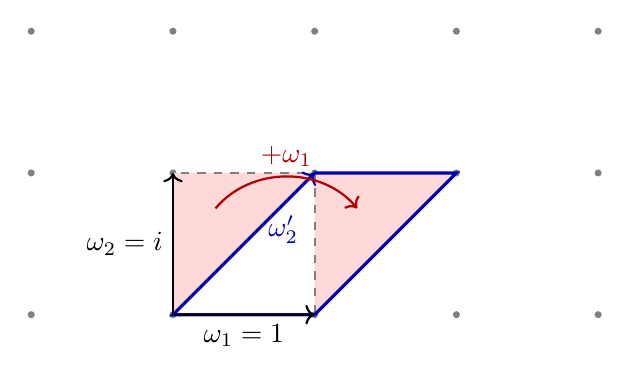
\begin{tikzpicture}[scale=1.8]
    \foreach \x in {-1,0,1,2,3} \foreach \y in {0,1,2} \fill[gray] (\x,\y) circle (0.025);
    \fill[red!15] (0,0) -- (1,1) -- (0,1) -- cycle;
    \fill[red!15] (1,0) -- (2,1) -- (1,1) -- cycle;
    \draw[gray, dashed, thick] (0,0) rectangle (1,1);
    \draw[very thick, blue!70!black] (0,0) -- (1,0) -- (2,1) -- (1,1) -- cycle;
    \draw[->, thick] (0,0) -- (1,0) node[midway, below] {$\omega_1 = 1$};
    \draw[->, thick] (0,0) -- (0,1) node[midway, left] {$\omega_2 = i$};
    \draw[->, thick, blue!70!black] (0,0) -- (1,1) node[pos=0.6, right] {$\omega_2'$};
    \draw[->, thick, red!70!black] (0.3,0.75) to[bend left=50] node[above] {$+\omega_1$} (1.3,0.75);
\end{tikzpicture}
\caption{$T$ による基底の取り替え $(\omega_1, \omega_2) \mapsto (\omega_1, \omega_2 + \omega_1)$（$\tau = i$ の場合、$\omega_2' = 1 + i$）。元の基本領域（破線の正方形）と新しい基本領域（青の平行四辺形）は、赤い三角形を $\omega_1$ だけ平行移動すれば互いに移り合う。トーラスでは $\omega_1$ だけ離れた点は同一視されているので、両者は同じトーラスである。}
\label{fig:T-cut-paste}
\end{figure}

\paragraph{群の作用であること}
1次分数変換の合成は行列の積に対応する：$\gamma, \gamma' \in SL(2,\mathbb{Z})$ に対して $\gamma(\gamma'\tau) = (\gamma\gamma')\tau$ が成り立つ（基底の取り替えを2回続けて行うことは、行列の積で表される1回の取り替えと同じである）。したがって $SL(2,\mathbb{Z})$ は $\mathbb{H}$ に\textbf{群として作用}し、その\textbf{軌道} $\{\gamma\tau \mid \gamma \in SL(2,\mathbb{Z})\}$ が「同じトーラスを表すラベル全体」となる。$\mathbb{H}/SL(2,\mathbb{Z})$ とは、この軌道の全体のことである。なお $-1 \in SL(2,\mathbb{Z})$ は $(\omega_1, \omega_2) \mapsto (-\omega_1, -\omega_2)$ であり、$\tau$ を変えない。

\begin{myex}{正方トーラス $\tau = i$ の軌道}{}
$\tau = i$（正方格子 $\mathbb{Z} + \mathbb{Z}i$）の軌道には、例えば
\begin{equation*}
    T(i) = 1 + i, \qquad -\frac{1}{i + 1} = \frac{-1 + i}{2}, \qquad \frac{i}{i + 1} = \frac{1 + i}{2}
\end{equation*}
などが含まれる。これらは見かけは異なる複素数だが、すべて同じ正方トーラスを表している（後2者の虚部が $1/2$ なのは、$\mathrm{Im}\,\tau' = \mathrm{Im}\,\tau/|c\tau+d|^2$ で $|i + 1|^2 = 2$ だからである）。一方、$S(i) = -1/i = i$ であり、$S$ は $\tau = i$ を動かさない。これは基底を $90^\circ$ 回転 $(\omega_1, \omega_2) = (1, i) \mapsto (i, -1)$ させても正方格子が自分自身に移ることを反映しており、正方トーラスが $z \mapsto iz$ という余分な自己同型を持つことに対応する。
\end{myex}

したがって、トーラスのモジュライ空間 $\mathcal{M}_{1}$ は、上半平面 $\mathbb{H}$ をモジュラー群で割った商空間
\begin{equation}
    \mathcal{M}_{1} = \mathbb{H} / SL(2, \mathbb{Z})
\end{equation}
となる。この商空間の形は、次の基本領域によって具体的に捉えられる。

\begin{myprop}{モジュラー群の基本領域}{fundamental-domain}
\begin{equation*}
    \mathcal{F} = \left\{ \tau \in \mathbb{H} \,\middle|\, |\tau| \ge 1,\ |\mathrm{Re}\,\tau| \le \tfrac{1}{2} \right\}
\end{equation*}
とおく。$\mathbb{H}$ の任意の点は、$SL(2, \mathbb{Z})$ の作用によって $\mathcal{F}$ の点に移る。さらに、$\mathcal{F}$ の内部の異なる2点が同じ軌道に属することはなく、同一視は境界上でのみ（$\mathrm{Re}\,\tau = \pm\frac12$ の2辺どうし、および円弧 $|\tau| = 1$ の左右の半分どうし）起こる。
\end{myprop}

\begin{proof}[証明の概略]
$\tau \in \mathbb{H}$ を固定する。$\mathrm{Im}(\gamma\tau) = \mathrm{Im}\,\tau / |c\tau + d|^2$ であり、$|c\tau + d| \le 1$ を満たす整数の組 $(c, d)$ は有限個しかないので、軌道上で $\mathrm{Im}$ は最大値をとる。その最大値を与える点に $T: \tau \mapsto \tau + 1$ を何回か施して $|\mathrm{Re}\,\tau| \le \frac12$ とする（$\mathrm{Im}$ は変わらない）。もし $|\tau| < 1$ なら、$S: \tau \mapsto -1/\tau$ により $\mathrm{Im}(-1/\tau) = \mathrm{Im}\,\tau/|\tau|^2 > \mathrm{Im}\,\tau$ となって最大性に反する。よって $|\tau| \ge 1$ であり、$\tau \in \mathcal{F}$ である。
\end{proof}

\begin{figure}[htbp]
\centering
\begin{tikzpicture}[scale=2]
    \fill[blue!10] (-0.5,0.866) arc (120:60:1) -- (0.5,2.2) -- (-0.5,2.2) -- cycle;
    \draw[->] (-1.4,0) -- (1.5,0) node[right] {$\mathrm{Re}\,\tau$};
    \draw[->] (0,0) -- (0,2.45) node[above] {$\mathrm{Im}\,\tau$};
    \draw[gray, dashed] (1,0) arc (0:180:1);
    \draw[gray, dashed] (-0.5,0) -- (-0.5,0.866);
    \draw[gray, dashed] (0.5,0) -- (0.5,0.866);
    \draw[very thick, blue!70!black] (-0.5,2.2) -- (-0.5,0.866) arc (120:60:1) -- (0.5,2.2);
    \node[below] at (-0.5,0) {$-\frac{1}{2}$};
    \node[below] at (0.5,0) {$\frac{1}{2}$};
    \node[below] at (1,0) {$1$};
    \node[below] at (-1,0) {$-1$};
    \fill (0,1) circle (0.03) node[below right] {$i$};
    \fill (0.5,0.866) circle (0.03) node[right] {$e^{i\pi/3}$};
    \fill (-0.5,0.866) circle (0.03) node[left] {$e^{2\pi i/3}$};
    \node at (0,1.6) {$\mathcal{F}$};
    \draw[<->, red!70!black] (-0.42,1.85) -- node[above, font=\scriptsize] {$T$ で同一視} (0.42,1.85);
    \draw[<->, red!70!black] (-0.3,1.08) to[bend left=40] node[above, font=\scriptsize] {$S$} (0.3,1.08);
    \node[above, font=\scriptsize] at (0,2.2) {$\uparrow$ カスプ $\tau \to i\infty$};
\end{tikzpicture}
\caption{モジュラー群 $SL(2,\mathbb{Z})$ の基本領域 $\mathcal{F}$（青）。左右の辺は $T: \tau \mapsto \tau + 1$ で、円弧の左右の半分は $S: \tau \mapsto -1/\tau$ で貼り合わされる。点 $i$ と $e^{i\pi/3}$（$\sim e^{2\pi i/3}$）は余分な対称性を持つ点であり、上方はカスプに向かって非コンパクトに伸びている。}
\label{fig:fundamental-domain}
\end{figure}

すなわち $\mathcal{M}_1$ は、$\mathcal{F}$ の境界を上の規則で貼り合わせた空間である（図\ref{fig:fundamental-domain}）。$\tau = i$ と $\tau = e^{i\pi/3}$ は特別な対称性を持つ点であり、そこでモジュライ空間は円錐特異点を持つ（第\ref{ch:group-action}章で詳しく調べる）。また、$\mathrm{Im}\,\tau \to \infty$ の方向（カスプ）にモジュライ空間は非コンパクトに伸びている。

\begin{note}
複素解析的には、楕円モジュラー関数 $j(\tau)$（$SL(2, \mathbb{Z})$ 不変な正則関数で、$\mathcal{F}$ の各点で異なる値をとる）によって
\begin{equation*}
    j: \mathbb{H}/SL(2, \mathbb{Z}) \xrightarrow{\ \cong\ } \mathbb{C}
\end{equation*}
という同一視が得られる。すなわち、粗モジュライ空間としては $\mathcal{M}_1$ は単なる複素平面であり、カスプ $\tau \to i\infty$ に1点 $j = \infty$ を加えれば $\mathbb{CP}^1$ にコンパクト化される。しかし、円錐特異点の情報（$\tau = i$ と $e^{i\pi/3}$ における余分な対称性）は $j$ によって見えなくなっており、それを記憶するにはオービフォールドやスタックの言葉が必要となる。
\end{note}

前節の定義に照らすと、$\mathcal{M}_1$ は微細モジュライ空間ではない。実際、すべてのトーラスは自己同型 $z \mapsto -z$ を持つ（これは $-1 \in SL(2, \mathbb{Z})$ が $\tau$ を動かさないことに対応する）。さらに並進 $z \mapsto z + c$ という連続的な自己同型もあるので、通常は原点を1点固定した\textbf{1点付きトーラス}（楕円曲線）のモジュライ空間 $\mathcal{M}_{1,1}$ を考える。本講義で $\mathcal{M}_1$ と書くときは、この $\mathcal{M}_{1,1}$ を指すものとする（第\ref{ch:deformation}章）。

\begin{note}
弦理論の摂動論（1ループ振幅）において、トーラスのモジュライ空間上の積分が実行される。ここでは2つの異なる無矛盾性の条件が現れる。第一に、Weyl変換でゲージ固定を行うためには、量子論的にWeyl対称性が保たれていなければならず、これは物質場とゴースト場の中心電荷の和が消えること $c_{\text{matter}} + c_{\text{ghost}} = 0$ を要求する。ボソン弦では $c_{\text{ghost}} = -26$ なので、時空の次元が臨界次元 $D = 26$ であることが要求される\cite{polchinskistringtheoryvolume12005}。第二に、積分が基本領域 $\mathcal{F}$ 上で矛盾なく定義されるためには、被積分関数がモジュラー変換で不変でなければならない（\textbf{モジュラー不変性}）。超弦理論のGSO射影は、この条件によって決まる\cite{polchinskistringtheoryvolume2005}。モジュライ空間の幾何学は、このように量子論の無矛盾性と直結している（第9章・第11章）。
\end{note}

\section{局所的な変形と大域的なトポロジーの概観}

モジュライ空間の構造は、局所的な性質と大域的な性質の2つの側面に分けて調べられる。

局所的には、ある状態をわずかに変形したときに、それが物理的に新しい状態（モジュライの別な点）を与えるか、それとも単なるゲージ変換（あるいは座標変換）に過ぎないかが問題になる。量子論の経路積分においては、モジュライ空間の接空間方向への変形は作用を変えない「零モード（ゼロ・モード）」に対応する。モジュライ空間が滑らかな点では、その次元は物理的な零モードの数に等しい。一般には、変形を記述するコホモロジー群 $H^0$（自己同型）、$H^1$（変形）、$H^2$（障害）の次元の交代和として\textbf{仮想次元}が定まり、これをトポロジカルに計算するのがAtiyah--Singerの指数定理である（第\ref{ch:deformation}章）。

一方、大域的には、モジュライ空間の境界や特異点が問題となる。前述のトーラスの例では、$\mathrm{Im}\,\tau \to \infty$ の極限でトーラスは無限に細長く退化し、1つのサイクルが潰れた「ピンチしたトーラス」（節点を1つ持つ曲線）に近づく。物理的には、これは弦理論の1ループ振幅における赤外領域（長いチューブを質量ゼロの粒子が伝播する極限）に対応しており、モジュライ空間を適切に「コンパクト化」して境界を制御しなければならない。この退化した曲線を境界として付け加えるのが、Deligne--Mumfordコンパクト化である（第10章）。

\begin{note}
相対論において計量を扱う際、本講義では $(-+++)$ の符号系を採用する。ローレンツ多様体の計量のモジュライを考える場合、空間成分と時間成分で許容される位相幾何学的性質（因果構造など）が異なるため、Riemann多様体（正定値計量）のモジュライとは異なる困難が生じる。弦理論では通常、Wick回転によってEuclid化された世界面や余剰次元の空間（Calabi--Yau多様体など）のモジュライを扱う（第\ref{ch:calabi-yau}章・第\ref{ch:gravity}章）。
\end{note}

\section{まとめ：物理学における役割と本講義の構成}

本章の総括として、モジュライ空間の概念が物理学の各分野でどのような役割を果たし、それが本講義のどの章に対応するかを整理しておく。

\paragraph{第I部：共通する数学的構造}
\begin{itemize}
    \item \textbf{群作用と商空間（第\ref{ch:group-action}章）}：ゲージ対称性による商。良い商が得られる条件、オービフォールド特異点、Gribov問題。
    \item \textbf{接空間・特異点・次元（第\ref{ch:deformation}章）}：零モードと変形複体のコホモロジー、倉西の局所モデル、指数定理。
    \item \textbf{束・接続・曲率（第\ref{ch:bundle}章）}：ゲージ場の幾何学的定式化と特性類。
\end{itemize}

\paragraph{第II部：物理に現れるモジュライ}
\begin{itemize}
    \item \textbf{ゲージ理論（第\ref{ch:instanton}章・第11章）}：Yang--Mills方程式のインスタントン解のモジュライ空間。モジュライ上の積分は、非摂動的な相関関数や量子異常（アノマリー）を記述する。
    \item \textbf{真空のモジュライ（第\ref{ch:vacuum}章）}：自発的対称性の破れと非線形シグマ模型、超対称ゲージ理論のシンプレクティック商・GIT商。
    \item \textbf{弦理論の余剰次元（第\ref{ch:calabi-yau}章）}：超弦理論のコンパクト化におけるCalabi--Yau多様体のモジュライ空間（複素構造とK\"ahler構造の変形）。これは低エネルギー有効理論におけるスカラー場（モジュライ場）として現れる。
    \item \textbf{一般相対論と2次元重力（第\ref{ch:gravity}章）}：計量の空間を微分同相で割った商。2次元ではTeichm\"uller空間とリーマン面のモジュライ $\mathcal{M}_g$ に帰着する。
\end{itemize}

\paragraph{第III部：発展的視点（予定）}
\begin{itemize}
    \item \textbf{共形場理論とリーマン面（第9章）}：Teichm\"uller空間と写像類群の商としてのリーマン面のモジュライ $\mathcal{M}_g$。弦の散乱振幅の導出の基礎となる。
\end{itemize}

\paragraph{付録}
\begin{itemize}
    \item \textbf{代数トポロジーの基礎（付録\ref{app:topology}）}：ホモトピーと被覆、基本群・高次ホモトピー群、写像度と巻き付き数、絡み数とHopf不変量、主束の自明性、de Rhamコホモロジー、ホモロジーと交点数、Euler数とBetti数。本文では初出の箇所から参照する。
    \item \textbf{超対称性の基礎（付録\ref{app:susy}）}：超対称性代数とBPS限界、多重項、$\mathcal{N}=1$ のラグランジアンと非繰り込み定理、$\mathcal{N}=2$ の特殊幾何。
    \item \textbf{弦理論の基礎（付録\ref{app:string}）}：Polyakov作用と臨界次元、種数展開、5つの超弦理論、T双対性、Dブレーン、双対性の網。
\end{itemize}

次章では、この「物理的冗長性を割って真の自由度を取り出す」という手続きを数学的に定式化する「群作用と商空間」について詳しく見ていく。

\chapter{群作用と商空間：ゲージ対称性との関係を理解する}
\label{ch:group-action}

第\ref{ch:intro}章では、モジュライ空間を「対象の集合を同値関係で割ったもの」として導入した。物理において同値関係の大部分は、ゲージ変換や座標変換といった\textbf{群の作用}によって与えられる。本章では、群作用と商空間の理論を整理し、商空間が良い空間になるための条件と、それが破れたときに現れる特異点や大域的障害を、具体例を通して調べる。

\section{ゲージ対称性と物理的冗長性}

物理系において「ゲージ対称性がある」という言明は、時空の並進対称性や回転対称性のような自然界に存在する「真の力学的な対称性」を意味するものではない。それは、我々が系を局所的かつ共変的に記述するために導入した力学変数（ゲージ場やベクトルポテンシャルなど）に、\textbf{物理的冗長性（Physical Redundancy）}が存在することを意味している。

例えば、非可換ゲージ理論（Yang--Mills理論）におけるゲージ場 $A_\mu(x) = A_\mu^a(x) T^a$ を考えよう。局所ゲージ変換
\begin{equation}
    A_\mu(x) \to A_\mu'(x) = U(x) A_\mu(x) U^{-1}(x) - \frac{i}{g} (\partial_\mu U(x)) U^{-1}(x)
    \label{eq:gauge-transf-ch2}
\end{equation}
（共変微分 $D_\mu = \partial_\mu - igA_\mu$ が共変的に変換されるように符号を選んだ）を施しても、系を規定する電磁場強度（曲率テンソル）
\begin{equation}
    F_{\mu\nu} = \partial_\mu A_\nu - \partial_\nu A_\mu - ig [A_\mu, A_\nu]
\end{equation}
は $F_{\mu\nu} \to U(x) F_{\mu\nu} U^{-1}(x)$ と共変的に変換され、ヤン・ミルズ作用 $S_{\text{YM}} \propto \int d^4x \, \text{Tr}(F_{\mu\nu}F^{\mu\nu})$ は完全に不変に保たれる。

この変換全体のなす群が\textbf{ゲージ変換群}である。$G$ をコンパクトなリー群（$U(1)$、$SU(N)$ など）とし、簡単のため時空 $M$ 上の自明な主 $G$ 束を考えると、ゲージ変換群は滑らかな写像 $U: M \to G$ 全体
\begin{equation}
    \mathcal{G} = \mathrm{Map}(M, G)
\end{equation}
に各点ごとの積 $(U_1 U_2)(x) = U_1(x) U_2(x)$ を入れたものであり、式 \eqref{eq:gauge-transf-ch2} によってゲージ接続全体の空間 $\mathcal{A}$ に作用する。

したがって、数学的に許容されるすべてのゲージ接続のなす空間（アフィン空間 $\mathcal{A}$）の中には、物理的に全く同一の状態を表す配位が無数に含まれていることになる。真に独立な物理的自由度からなる空間（モジュライ空間）は、無限次元のリー群 $\mathcal{G}$ の作用によって $\mathcal{A}$ を割った商空間として定義されなければならない。
\begin{equation}
    \mathcal{M} = \mathcal{A} / \mathcal{G}
\end{equation}

最も簡単な電磁気学（$G = U(1)$）の場合、ゲージ変換は見慣れた $A_\mu \to A_\mu + \frac{1}{g}\partial_\mu\lambda$ となり、時空が単連結であれば、2つのポテンシャルが同じ軌道に属するのは、その差が完全形式であるときに限る。単連結でない場合には、$\lambda$ が一価でない（$U = e^{i\lambda}$ は一価だが $\lambda$ は $2\pi$ の整数倍だけずれうる）「大きな」ゲージ変換が存在し、差は周期が $2\pi/g$ の整数倍となる閉形式まで許される（第\ref{ch:deformation}章のトーラス上の平坦接続の例を参照）。

\begin{note}
$U(x) = e^{i\lambda(x)}$ を式 \eqref{eq:gauge-transf-ch2} に代入する。$U(1)$ は可換なので $U A U^{-1} = A$ であり、$(\partial_\mu U) U^{-1} = i\partial_\mu\lambda$ より
\begin{equation*}
    A_\mu \to A_\mu - \frac{i}{g}(i\partial_\mu \lambda) = A_\mu + \frac{1}{g}\partial_\mu \lambda
\end{equation*}
を得る。したがって $A' - A = \frac{1}{g}d\lambda$ は完全形式である。
\end{note}

\begin{note}
\textbf{基本群}・\textbf{単連結}（任意のループが1点に縮められること）は付録\ref{sec:topo-pi1}節、\textbf{閉形式}（$d\alpha = 0$）・\textbf{完全形式}（$\alpha = d\beta$）と\textbf{de Rhamコホモロジー}は付録\ref{sec:topo-derham}節を参照。ここで必要なのは「$M$ が単連結ならば、閉1形式はすべて完全形式である」という事実である。

本文の状況では、同じ場の強さを与える2つのポテンシャルの差 $A' - A$ は閉形式（$d(A' - A) = F' - F = 0$）である。それが完全形式なら $\lambda$ を一価な関数として選べ、通常のゲージ変換で結ばれる。単連結でない場合に現れる「大きな」ゲージ変換では、$U = e^{i\lambda}$ は一価だが $\lambda$ 自身は偏角 $\varphi$ のように一価でなく、$A' - A = \frac{1}{g}d\lambda$ は完全形式でない閉形式となる。
\end{note}

ここで商空間 $\mathcal{A}/\mathcal{G}$ の構造は、時空のトポロジーに依存する。$M = \mathbb{R}^4$ のように可縮な時空では、Poincar\'eの補題により「$dF = 0$ を満たす $F$ は必ず $F = dA$ と書け、$F$ が同じなら $A$ はゲージ同値」であるから、$\mathcal{A}/\mathcal{G}$ は閉2形式 $F$ の空間と同一視され、場の強さ $F$ がすべての物理的情報を持つ。一方、$M$ が非自明なループ（例えば $S^1$ 方向）を持つ場合はそうではない。$F = 0$ でもホロノミー $e^{ig\oint A}$ が非自明な配位は、自明な配位 $A = 0$ とゲージ同値ではない。これがAharonov--Bohm効果であり、第\ref{ch:deformation}章ではこれをWilsonラインのモジュライとして再び扱う。

\begin{note}
\textbf{可縮}（空間を連続的に1点に縮められること）と\textbf{Poincar\'eの補題}（可縮な領域では次数 $k \ge 1$ の閉形式はすべて完全形式）については付録\ref{sec:topo-homotopy}節・\ref{sec:topo-derham}節を参照。$k = 2$ の場合を本文に適用すると、$dF = 0$ を満たす $F$ は必ず $F = dA$ と書け、また $F$ が同じ2つのポテンシャルの差は閉1形式なので完全形式、すなわちゲージ変換で結ばれる。
\end{note}

\begin{note}
この「物理的冗長性を割る」という幾何学的な要請は、量子論の経路積分において極めて具体的な手続きを要求する。分配関数においてゲージ軌道の体積で割る操作を行う際、ゲージ固定条件のヤコビアンとしてFaddeev--Popov行列式が現れる。これを局所的な作用に持ち上げるために導入されるのが、反交換関係を満たすグラスマン偶奇性を持ったゴースト場・反ゴースト場である。ゴースト場は、商空間 $\mathcal{M} = \mathcal{A} / \mathcal{G}$ 上の積分測度を正しく定義し、量子論レベルでのBRST不変性を保証するための代数的な要請として不可欠である。
\end{note}


\section{群作用の数学的定式化：軌道と商空間}

前節で見たモジュライ空間 $\mathcal{M}$ を構成する数学的基盤として、群作用の理論を整理しておく。以下、$M$ は物理においては「すべての許容される場の配位空間」や「計量の空間」、$G$ は「ゲージ群」や「微分同相群」を念頭に置いている。

\subsection{群作用・軌道・商空間}

\begin{mydef}{群作用}{}
群 $G$ と集合 $M$ に対し、写像 $\Phi: G \times M \to M$、$(g, x) \mapsto g \cdot x$ が
\begin{enumerate}
    \item $e \cdot x = x$ \quad（$e$ は単位元）
    \item $g \cdot (h \cdot x) = (gh) \cdot x$ \quad（$g, h \in G$）
\end{enumerate}
を満たすとき、$\Phi$ を $G$ の $M$ への\textbf{（左）作用}という。$G$ がリー群、$M$ が滑らかな多様体で $\Phi$ が滑らかなとき、\textbf{滑らかな作用}という。
\end{mydef}

各 $g \in G$ に対して $x \mapsto g \cdot x$ は逆写像 $x \mapsto g^{-1} \cdot x$ を持つので、滑らかな作用の場合、これは $M$ の微分同相写像である。

\begin{mydef}{軌道・固定部分群・商空間}{}
\begin{enumerate}
    \item $x \in M$ の\textbf{軌道（Orbit）}を $G \cdot x = \{ g \cdot x \mid g \in G \} \subset M$ で定める。
    \item $x \in M$ の\textbf{固定部分群（等方部分群、スタビライザー）}を $G_x = \{ g \in G \mid g \cdot x = x \}$ で定める。
    \item $M$ 上の関係 $\sim$ を「$x \sim y \iff$ ある $g \in G$ が存在して $y = g \cdot x$」で定義し、その同値類の集合を\textbf{商空間} $M/G$、$x$ をその同値類に写す写像を\textbf{射影} $\pi: M \to M/G$ と呼ぶ。$M/G$ には\textbf{商位相}（$V \subset M/G$ が開集合 $\iff$ $\pi^{-1}(V)$ が $M$ の開集合）を入れる。
\end{enumerate}
\end{mydef}

固定部分群は、物理的には配位 $x$ を変えない「残された対称性」を表している。

定義の中で $\sim$ を同値関係と呼んだが、これは実際に同値関係であり、したがって $M$ は互いに交わらない軌道の和に分割され、$M/G$ は「軌道の集合」と同一視される。
\begin{proof}
反射律は $x = e \cdot x$ から、対称律は $y = g \cdot x \Rightarrow x = g^{-1} \cdot y$ から、推移律は $y = g \cdot x,\ z = h \cdot y \Rightarrow z = (hg) \cdot x$ から従う。
\end{proof}

また、作用が連続ならば射影 $\pi: M \to M/G$ は連続な開写像である。この性質は後でハウスドルフ性を調べる際に用いる。
\begin{proof}
連続性は商位相の定義から従う。$V \subset M$ を開集合とすると、
\begin{equation*}
    \pi^{-1}(\pi(V)) = \bigcup_{g \in G} g \cdot V
\end{equation*}
であり、各 $g \cdot V$ は（$x \mapsto g\cdot x$ が同相写像なので）開集合である。よって $\pi(V)$ は開集合である。
\end{proof}

\subsection{固定部分群と軌道の構造}

軌道と固定部分群の間には、次の基本的な関係がある。

\begin{myprop}{軌道・固定部分群定理}{orbit-stabilizer}
\begin{enumerate}
    \item $G_x$ は $G$ の部分群である。
    \item 写像 $G/G_x \to G \cdot x$、$g G_x \mapsto g \cdot x$ は well-defined な全単射である。
    \item 同じ軌道上の点の固定部分群は互いに共役である：$G_{g \cdot x} = g\, G_x\, g^{-1}$。
\end{enumerate}
\end{myprop}
\begin{proof}
(1) $g, h \in G_x$ ならば $(gh^{-1}) \cdot x = g \cdot (h^{-1} \cdot x) = g \cdot x = x$。
(2) $g \cdot x = h \cdot x \iff h^{-1}g \in G_x \iff g G_x = h G_x$ より、well-defined性と単射性が同時に従う。全射性は軌道の定義から明らか。
(3) $k \in G_x$ ならば $(g k g^{-1}) \cdot (g \cdot x) = g \cdot (k \cdot x) = g \cdot x$ であり、逆も同様。
\end{proof}

$G$ がリー群で作用が滑らかなとき、$G_x$ は閉部分群（したがってリー部分群）であり、(2) から
\begin{equation}
    \dim (G \cdot x) = \dim G - \dim G_x
\end{equation}
が成り立つ。すなわち、固定部分群が大きい点ほど軌道は「小さく」なる。また (3) により、軌道ごとに固定部分群の共役類が定まる。これを軌道の\textbf{型}と呼ぶ。以下、いくつかの例でこれらの概念を確認しよう。

\paragraph{例：平面の回転 $U(1) \curvearrowright \mathbb{C}$}
$U(1)$ を $e^{i\theta} \cdot z = e^{i\theta} z$ によって $\mathbb{C}$ に作用させる。$z \neq 0$ の軌道は半径 $|z|$ の円周で固定部分群は自明（$G_z = \{1\}$）、原点の軌道は1点 $\{0\}$ で固定部分群は $G_0 = U(1)$ 全体である。軌道の次元はそれぞれ $1 - 0 = 1$ と $1 - 1 = 0$ で、上の公式と整合している。不変量 $r = |z|$ によって商空間は
\begin{equation}
    \mathbb{C}/U(1) \cong [0, \infty)
\end{equation}
となる。これは境界を持つ半直線であり、境界点 $r = 0$ がちょうど固定部分群の大きい点に対応している。物理的には、$U(1)$ 対称性を持つ複素スカラー場 $\phi$ の配位を対称性で割ると不変量 $|\phi|$ だけが残り、$\phi = 0$ で対称性が回復することに対応する（第\ref{ch:vacuum}章）。

\paragraph{例：円周 $\mathbb{Z} \curvearrowright \mathbb{R}$}
$\mathbb{Z}$ を $n \cdot x = x + n$ によって $\mathbb{R}$ に作用させる。$n \neq 0$ ならば $x + n \neq x$ なので固定部分群はすべて自明であり、商空間は $\mathbb{R}/\mathbb{Z} \cong S^1$ という滑らかな多様体となる。周期的境界条件を課すことは、この商をとることに他ならない。

\subsection{例：複素射影空間とHopf束}
\label{subsec:cpn-hopf}

前の2つの例は「商をとると何が起こるか」を示す最小の例であったが、本節で導入した概念（軌道・固定部分群・商位相）がすべて非自明に、しかも物理と直結した形で現れるのが複素射影空間 $\mathbb{CP}^n$ とHopf束である。本講義では、この例が繰り返し登場する：Diracモノポール（第\ref{ch:bundle}章）、$\mathbb{CP}^{N-1}$ 模型と真空のモジュライ（第\ref{ch:vacuum}章）、Calabi--Yau多様体を定義する周囲の空間（第\ref{ch:calabi-yau}章）である。

\paragraph{動機：量子力学の状態空間}
$(n+1)$ 準位の量子系の状態はベクトル $\psi \in \mathbb{C}^{n+1} \setminus \{0\}$ で表されるが、$\psi$ と $\lambda \psi$（$\lambda \in \mathbb{C}^\times$）は同じ物理状態を表す。実際、期待値
\begin{equation}
    \langle O \rangle_\psi = \frac{\psi^\dagger O \psi}{\psi^\dagger \psi}
\end{equation}
は $\psi \to \lambda\psi$ で不変であり、ノルム $|\lambda|$ と全体の位相 $\arg\lambda$ はどちらも観測にかからない。したがって純粋状態の空間は「ベクトルの空間」ではなく、その $\mathbb{C}^\times$ による商、すなわち原点を通る複素直線（\textbf{射線}）の空間である。これは「物理的に区別できない記述を同一視して真の自由度を取り出す」という、本章の主題の最も素朴な例になっている。

\begin{mydef}{複素射影空間}{}
$\mathbb{C}^\times = \mathbb{C} \setminus \{0\}$ を $\lambda \cdot z = \lambda z$ によって $\mathbb{C}^{n+1} \setminus \{0\}$ に作用させたときの商空間
\begin{equation*}
    \mathbb{CP}^n = (\mathbb{C}^{n+1} \setminus \{0\}) / \mathbb{C}^\times
\end{equation*}
を\textbf{複素射影空間}という。$z = (z_0, \dots, z_n)$ の同値類を $[z_0 : z_1 : \cdots : z_n]$ と書き、\textbf{斉次座標}と呼ぶ。
\end{mydef}

軌道・固定部分群の言葉で整理しておこう。$z \neq 0$ の軌道 $\mathbb{C}^\times \cdot z$ は、$z$ を通る複素直線から原点を除いたものである。また $\lambda z = z$ かつ $z \neq 0$ ならば、$z_i \neq 0$ となる成分で比べて $\lambda = 1$ となるので、固定部分群はすべて自明、すなわちこの作用は\textbf{自由}である。原点を除いたのは、原点が固定部分群 $\mathbb{C}^\times$ 全体を持つ唯一の点であり、しかもその軌道 $\{0\}$ がすべての軌道の閉包に含まれる（$\lambda \to 0$ とすればよい）からである。原点を残すと、商空間で原点の像はすべての点の近傍に入り込み、ハウスドルフ性が失われる。これは前節の平面の回転の例で原点が境界点を与えたのと同じ現象の、より深刻な版であり、第\ref{ch:vacuum}章のGIT商における「不安定点を除く」操作の原型でもある。

\paragraph{アフィン座標近傍：多様体としての構造}
$\mathbb{CP}^n$ が実際に複素 $n$ 次元の多様体であることは、具体的な座標を書けば直接確かめられる。$i = 0, \dots, n$ に対して開集合
\begin{equation}
    U_i = \{ [z] \in \mathbb{CP}^n \mid z_i \neq 0 \}
\end{equation}
をとる（条件 $z_i \neq 0$ は代表元の取り方によらない）。$U_i$ 上では $z_i$ で割って代表元を $z_i = 1$ と正規化できるので、
\begin{equation}
    \varphi_i : U_i \to \mathbb{C}^n, \qquad [z_0 : \cdots : z_n] \mapsto \left( \frac{z_0}{z_i}, \dots, \widehat{\frac{z_i}{z_i}}, \dots, \frac{z_n}{z_i} \right)
\end{equation}
（$\widehat{\ }$ は除くことを表す）は全単射であり、これを\textbf{アフィン座標}（非斉次座標）と呼ぶ。$\{U_i\}_{i=0}^n$ は $\mathbb{CP}^n$ を覆い、重なり $U_i \cap U_j$ での座標変換は
\begin{equation}
    \frac{z_k}{z_j} = \frac{z_k / z_i}{z_j / z_i}
\end{equation}
すなわち「アフィン座標の1つ $w_j = z_j/z_i$ で他を割る」という正則写像である（$U_i \cap U_j$ 上では $w_j \neq 0$）。したがって $\mathbb{CP}^n$ は複素 $n$ 次元（実 $2n$ 次元）の\textbf{複素多様体}となる。「代表元を $z_i = 1$ と正規化する」という操作は、各軌道とちょうど1点で交わる横断面（スライス）$\{z_i = 1\}$ を選ぶことであり、ゲージ固定の有限次元版にほかならない。ただし、どの1つのスライスも $\{z_i = 0\}$ 上の軌道とは交わらないので、全体を覆うには $n+1$ 枚が必要である。

また、$\mathbb{CP}^n$ は $U_0 \cong \mathbb{C}^n$ と、その補集合 $\{z_0 = 0\} \cong \mathbb{CP}^{n-1}$ に分解される。これを繰り返すと
\begin{equation}
    \mathbb{CP}^n = \mathbb{C}^n \sqcup \mathbb{C}^{n-1} \sqcup \cdots \sqcup \mathbb{C}^1 \sqcup \mathbb{C}^0
\end{equation}
となり、$\mathbb{CP}^n$ は $\mathbb{C}^n$ に「無限遠の $\mathbb{CP}^{n-1}$」を付け加えてコンパクト化したものとみなせる。各 $\mathbb{C}^k$ は実 $2k$ 次元の胞体であり、偶数次元の胞体しかないことから、Euler数は $\chi(\mathbb{CP}^n) = n + 1$ となる。特に $n = 1$ では $\mathbb{CP}^1 = \mathbb{C} \cup \{\infty\}$（\textbf{Riemann球面}）であり、第\ref{ch:intro}章でトーラスのモジュライ空間を $j$ 不変量でコンパクト化したときに現れたのもこの空間であった。

\begin{note}
\textbf{胞体}（開球体と同相な部分）への分割と、胞体の数の交代和としての\textbf{Euler数} $\chi = c_0 - c_1 + c_2 - \cdots$ については付録\ref{sec:topo-euler}節を参照。$\mathbb{CP}^n$ は各偶数次元に1つずつ胞体を持つので $\chi = n + 1$ であり、$n = 1$ では $\chi(S^2) = 2$ と一致する。
\end{note}

\paragraph{2段階の商：$\mathbb{C}^\times = \mathbb{R}_{>0} \times U(1)$}
$\mathbb{C}^\times$ は極形式 $\lambda = r e^{i\theta}$ により $\mathbb{R}_{>0} \times U(1)$ と分解される。これに対応して、商も2段階に分けてとることができる。まず
\begin{equation}
    \mathbb{C}^{n+1} \setminus \{0\} \xrightarrow{\ \cong\ } \mathbb{R}_{>0} \times S^{2n+1}, \qquad z \mapsto \left( |z|,\ \frac{z}{|z|} \right)
\end{equation}
は微分同相であり、$\mathbb{R}_{>0}$ はこの第1因子に掛け算で自由かつ推移的に作用する。したがって $\mathbb{R}_{>0}$ による商は単位球面 $S^{2n+1} = \{ |z| = 1 \}$ そのものである。言い換えれば、「$|z| = 1$ と正規化する」ことは $\mathbb{R}_{>0}$ 部分に対する\textbf{大域的な}ゲージ固定であり、ここには何の障害もない。残る $U(1)$ は $S^{2n+1}$ を保つので、
\begin{equation}
    \mathbb{CP}^n \cong S^{2n+1} / U(1), \qquad e^{i\theta} \cdot z = e^{i\theta} z
\end{equation}
を得る（図\ref{fig:rpn-analog}）。

\begin{note}
上の同一視が位相空間として正しいことを確かめておく。包含 $S^{2n+1} \hookrightarrow \mathbb{C}^{n+1} \setminus \{0\}$ は連続写像 $S^{2n+1}/U(1) \to (\mathbb{C}^{n+1} \setminus \{0\})/\mathbb{C}^\times$ を誘導し、これは全単射である（各 $\mathbb{C}^\times$ 軌道は $S^{2n+1}$ とちょうど1つの $U(1)$ 軌道で交わる）。逆写像は連続写像 $z \mapsto [z/|z|]$ から誘導されるので連続である。
\end{note}

この表示から、$\mathbb{CP}^n$ の大域的な性質がただちに従う。
\begin{itemize}
    \item \textbf{コンパクト性}：$\mathbb{CP}^n$ はコンパクト空間 $S^{2n+1}$ の連続像である。
    \item \textbf{ハウスドルフ性}：$U(1)$ はコンパクトなので作用は固有であり、次節で示すように商はハウスドルフである。（$\mathbb{C}^\times$ はコンパクトではないが、$|\lambda| = |\lambda z| / |z|$ が上下から押さえられることから $\mathbb{C}^\times \curvearrowright \mathbb{C}^{n+1} \setminus \{0\}$ も直接固有であることが確かめられる。）
    \item \textbf{主束の構造}：$U(1) \curvearrowright S^{2n+1}$ は自由かつ固有なので、次節の商多様体定理により $\pi : S^{2n+1} \to \mathbb{CP}^n$ は主 $U(1)$ 束となり、$\dim_{\mathbb{R}} \mathbb{CP}^n = (2n+1) - 1 = 2n$ はアフィン座標による計算と一致する。
\end{itemize}

この2段階の構成は、第\ref{ch:vacuum}章で重要になる構造の原型である。$\mathbb{C}^\times$ は $U(1)$ の複素化であり、「$\mathbb{C}^\times$ で割る」（GIT商）ことと「$|z|^2 = \xi$ という条件を課してから $U(1)$ で割る」（シンプレクティック商）ことが同じ空間を与える。$|z|^2$ は $U(1)$ 作用のモーメント写像であり、$\xi > 0$ はFIパラメータとして $\mathbb{CP}^n$ の大きさを決める（Kempf--Nessの定理 \ref{thm:kempf-ness}）。

\begin{figure}[htbp]
\centering
\begin{tikzpicture}[scale=1.3]
    \foreach \a in {15,60,105,150} {
        \draw[gray!70] ({-2*cos(\a)},{-2*sin(\a)}) -- ({2*cos(\a)},{2*sin(\a)});
    }
    \draw[very thick, blue!70!black] ({-2*cos(35)},{-2*sin(35)}) -- ({2*cos(35)},{2*sin(35)}) node[above right, font=\scriptsize] {軌道 $\mathbb{R}^\times \cdot x$};
    \draw[thick] (0,0) circle (1);
    \fill[white] (0,0) circle (0.05);
    \draw (0,0) circle (0.05);
    \fill[red!70!black] ({cos(35)},{sin(35)}) circle (0.06) node[below right, font=\scriptsize] {$x/|x|$};
    \fill[red!70!black] ({-cos(35)},{-sin(35)}) circle (0.06) node[above left, font=\scriptsize] {$-x/|x|$};
    \draw[red!70!black, dashed, <->] ({cos(35)-0.12},{sin(35)+0.1}) to[bend right=50] ({-cos(35)+0.02},{-sin(35)+0.15});
    \node[font=\scriptsize] at (1.3,-0.95) {$S^1 = \{|x| = 1\}$};
\end{tikzpicture}
\caption{2段階の商の実数版：$\mathbb{RP}^1 = (\mathbb{R}^2 \setminus \{0\})/\mathbb{R}^\times$。各軌道（原点を除いた直線、青）は、まず $\mathbb{R}_{>0}$ で割ると単位円上の対蹠点の組（赤）になり、残る $\{\pm 1\} = O(1)$ でこれを同一視して1点になる。複素数の場合は $\{\pm 1\}$ が $U(1)$ に置き換わり、単位球面 $S^{2n+1}$ 上の各軌道は円周となる。}
\label{fig:rpn-analog}
\end{figure}

\paragraph{等質空間としての $\mathbb{CP}^n$}
軌道・固定部分群定理（命題\ref{prop:orbit-stabilizer}）を用いると、$\mathbb{CP}^n$ を別の群の商として表すこともできる。ユニタリ群 $U(n+1)$ は $\mathbb{C}^{n+1}$ に行列の積で作用し、スカラー倍と可換なので $\mathbb{CP}^n$ に作用する。$U(n+1)$ は単位球面 $S^{2n+1}$ 上に推移的に作用する（任意の単位ベクトルは、それを第1列とするユニタリ行列によって $e_0 = (1, 0, \dots, 0)$ から写される）ので、$\mathbb{CP}^n$ 上でも推移的である。点 $[e_0] = [1 : 0 : \cdots : 0]$ の固定部分群は、$g e_0 = \lambda e_0$ となる $g \in U(n+1)$ の全体であり、ユニタリ行列は $e_0$ の直交補空間を保つので
\begin{equation}
    U(n+1)_{[e_0]} = \left\{ \begin{pmatrix} \lambda & 0 \\ 0 & h \end{pmatrix} \,\middle|\, \lambda \in U(1),\ h \in U(n) \right\} \cong U(1) \times U(n)
\end{equation}
である。したがって
\begin{equation}
    \mathbb{CP}^n \cong \frac{U(n+1)}{U(1) \times U(n)} \cong \frac{SU(n+1)}{S(U(1) \times U(n))}
\end{equation}
であり、次元は $(n+1)^2 - 1 - n^2 = 2n$ と正しく合う。物理的には、$SU(n+1)$ 対称な理論で真空が $S(U(1) \times U(n))$ まで自発的に破れたとき、真空の多様体（コセット空間 $G/H$）がまさに $\mathbb{CP}^n$ になることを意味する（第\ref{ch:vacuum}章の $\mathbb{CP}^{N-1}$ 模型）。量子力学の言葉では、「任意の純粋状態は適当なユニタリ変換で基準状態 $e_0$ に移せ、$e_0$ を（位相を除いて）変えないユニタリ変換は $U(1) \times U(n)$ である」ということである。

\paragraph{$n = 1$：Riemann球面・Bloch球面とHopf写像}
$n = 1$ の場合を具体的に見よう。$z = (z_0, z_1) \in S^3$（$|z_0|^2 + |z_1|^2 = 1$）に対し、Pauli行列 $\sigma_a$ を用いて
\begin{equation}
    \pi(z) = \bm{x} = (x_1, x_2, x_3), \qquad x_a = z^\dagger \sigma_a z
    \label{eq:hopf-map}
\end{equation}
と定める。成分で書けば
\begin{equation}
    x_1 + i x_2 = 2\,\bar{z}_0 z_1, \qquad x_3 = |z_0|^2 - |z_1|^2
\end{equation}
である。このとき
\begin{equation}
    |\bm{x}|^2 = 4|z_0|^2|z_1|^2 + \left( |z_0|^2 - |z_1|^2 \right)^2 = \left( |z_0|^2 + |z_1|^2 \right)^2 = 1
\end{equation}
なので $\pi$ は $S^3 \to S^2$ という写像であり、$z \to e^{i\alpha}z$ で明らかに不変である。逆に、$\bm{x} \in S^2$ を極座標 $(\theta, \phi)$ で表すと、
\begin{equation}
    \pi^{-1}(\bm{x}) = \left\{ e^{i\alpha} \left( \cos\frac{\theta}{2},\ e^{i\phi}\sin\frac{\theta}{2} \right) \,\middle|\, \alpha \in [0, 2\pi) \right\}
    \label{eq:hopf-fiber}
\end{equation}
となり（$x_3 = \cos^2\frac{\theta}{2} - \sin^2\frac{\theta}{2} = \cos\theta$、$x_1 + ix_2 = 2\cos\frac{\theta}{2}\sin\frac{\theta}{2}\,e^{i\phi} = \sin\theta\, e^{i\phi}$ より確かめられる）、各点の逆像はちょうど1つの $U(1)$ 軌道である。したがって $\pi$ は同相 $S^3/U(1) \cong S^2$ を誘導する。この $\pi$ を\textbf{Hopf写像}、主 $U(1)$ 束 $\pi : S^3 \to S^2$ を\textbf{Hopf束}（Hopfファイブレーション）と呼ぶ。

同じ空間には3つの見方がある。
\begin{itemize}
    \item \textbf{Riemann球面}：アフィン座標 $w = z_1/z_0 \in \mathbb{C} \cup \{\infty\}$ は、上の表示では $w = \tan\frac{\theta}{2}\, e^{i\phi}$ であり、これは $S^2$ の南極からの立体射影 $w = (x_1 + ix_2)/(1 + x_3)$ に一致する。北極 $\theta = 0$ が $w = 0$、南極 $\theta = \pi$ が $w = \infty$ に対応する。
    \item \textbf{Bloch球面}：スピン $1/2$ の状態 $\psi = (z_0, z_1)^T$ に対し、\eqref{eq:hopf-map} の $\bm{x}$ はスピンの期待値 $\langle \bm{\sigma} \rangle_\psi$ そのものである。\eqref{eq:hopf-fiber} の状態は $\bm{x} \cdot \bm{\sigma}$ の固有値 $+1$ の固有状態、すなわち「$\bm{x}$ 方向を向いたスピン」であり、全体の位相 $e^{i\alpha}$ が $U(1)$ ファイバーの方向である。
    \item \textbf{等質空間}：上の一般論で $n = 1$ とすると $S^2 \cong SU(2)/U(1)$。$SU(2)$ の $S^2$ への作用は、Bloch球面の回転（$SU(2) \to SO(3)$）にほかならない。
\end{itemize}

\paragraph{局所切断と推移関数：大域的なゲージ固定の不可能性}
$U(1)$ による商に対して「ゲージ固定」、すなわち各ファイバーから1点を選ぶことを試みよう。$S^2$ を2つの開集合
\begin{equation}
    U_N = S^2 \setminus \{\text{南極}\} = \{z_0 \neq 0\}, \qquad U_S = S^2 \setminus \{\text{北極}\} = \{z_1 \neq 0\}
\end{equation}
で覆う。$U_N$ 上では「$z_0$ が正の実数」という条件でファイバーの点がただ1つ決まり、$U_S$ 上では「$z_1$ が正の実数」で決まる。すなわち局所切断
\begin{align}
    s_N(\theta, \phi) &= \frac{|z_0|}{z_0}\, z = \left( \cos\frac{\theta}{2},\ e^{i\phi}\sin\frac{\theta}{2} \right) && (\theta < \pi), \\
    s_S(\theta, \phi) &= \frac{|z_1|}{z_1}\, z = \left( e^{-i\phi}\cos\frac{\theta}{2},\ \sin\frac{\theta}{2} \right) && (\theta > 0)
\end{align}
が得られる（$s_N$ は $\theta = 0$ で $\phi$ によらず $(1, 0)$ となり滑らかである。$s_S$ についても同様）。これらはそれぞれの定義域で局所自明化
\begin{equation}
    \pi^{-1}(U_N) \xrightarrow{\ \cong\ } U_N \times U(1), \qquad z \mapsto \left( \pi(z),\ \frac{z_0}{|z_0|} \right)
\end{equation}
（$U_S$ についても同様）を与える。重なり $U_N \cap U_S$ では
\begin{equation}
    s_S = s_N \cdot e^{-i\phi}
    \label{eq:hopf-transition}
\end{equation}
であり、推移関数 $e^{-i\phi}$ は赤道 $S^1$ を $U(1)$ にちょうど1回（向きを逆に）巻き付ける写像である。これは第\ref{ch:bundle}章のDiracモノポールの推移関数 $t_{NS} = e^{in\phi}$ で $|n| = 1$ としたものにほかならない。

$s_N$ を南極まで延長しようとすると、$\theta \to \pi$ で $s_N \to (0, e^{i\phi})$ となって極限が $\phi$ に依存し、連続に延長できない。これは偶然ではなく、\textbf{Hopf束には大域的な切断が存在しない}。実際、大域的な切断があれば主束は自明となり $S^3 \cong S^2 \times S^1$ となるが、$S^3$ は単連結で、$S^2 \times S^1$ の基本群は $\mathbb{Z}$ なのでこれは不可能である。すなわち「$\mathbb{R}_{>0}$ 部分は $|z| = 1$ で大域的にゲージ固定できたが、$U(1)$ 部分はどうやっても大域的にはゲージ固定できない」。ゲージ固定条件 $\arg z_0 = 0$ が破綻する南極は、Diracモノポールにおける\textbf{Diracの弦}の位置にほかならない。これは、本章の後半で扱うGribov問題とSingerの定理（大域的切断の非存在）の、最も簡単な有限次元版である。

\begin{note}
ここでは3つの事実を用いた。(1)「大域的切断が存在する $\iff$ 主束が自明」（付録の命題\ref{prop:section-trivial}）。すなわち、大域的にゲージを固定できることと束が自明であることは同じである。(2)「$S^3$ は単連結」、(3)「$\pi_1(S^2 \times S^1) \cong \mathbb{Z}$」（いずれも付録\ref{sec:topo-pi1}節）。基本群は位相不変量なので、$S^3$ と $S^2 \times S^1$ は同相ではありえない。
\end{note}

\paragraph{ファイバーの絡み目}
Hopf束の非自明さは、ファイバーの配置として目で見ることもできる。\eqref{eq:hopf-fiber} より各ファイバーは $S^3$ 内の大円である。$S^3 \subset \mathbb{C}^2 = \mathbb{R}^4$ を、$(z_0, z_1) = (0, i)$ からの立体射影で $\mathbb{R}^3 \cup \{\infty\}$ に写すと、北極上のファイバー $\{z_1 = 0\}$ は単位円周に、南極上のファイバー $\{z_0 = 0\}$ は射影の中心を通るので直線（$x_3$ 軸 $\cup \{\infty\}$）に写る（図\ref{fig:hopf-link}）。単位円周は $x_3$ 軸のまわりを1周しているので、2つのファイバーは\textbf{絡み数1}で絡み合っている。一般に、$S^2$ の任意の異なる2点上のファイバーは互いに1回絡み合い、その他のファイバーは $|z_0| = \text{一定}$ で定まる入れ子状のトーラス上を、両方向にそれぞれ1回ずつ巻く円周（Villarceau円）として現れる。この絡み数は\textbf{Hopf不変量}と呼ばれ、Hopf写像は $\pi_3(S^2) \cong \mathbb{Z}$ の生成元を与える。高次元の球面から低次元の球面への写像が非自明でありうることを示した、歴史的にも重要な例である。

\begin{note}
\textbf{ホモトピー群} $\pi_n$（$S^n$ からの写像の連続変形による分類）、\textbf{絡み数}、\textbf{Hopf不変量}については付録\ref{sec:topo-pin}節・\ref{sec:topo-hopf}節を参照。付録では、Hopf束のホモトピー完全列から $\pi_3(S^2) \cong \pi_3(S^3) \cong \mathbb{Z}$ が導かれること、Hopf不変量がChern--Simons形式の積分 $\int A \wedge dA$ で書けること（Whiteheadの公式）も説明する。
\end{note}

\begin{figure}[htbp]
\centering
\begin{tikzpicture}[scale=1.2]
    % 円周（北極上のファイバー）の後ろ半分
    \draw[very thick, blue!70!black] (1.6,0) arc (0:180:1.6 and 0.5);
    % x3軸（南極上のファイバー）
    \draw[very thick, red!70!black] (0,-2) -- (0,-0.6);
    \draw[very thick, red!70!black, ->] (0,-0.4) -- (0,2.1) node[above, black, font=\scriptsize] {$x_3$ 軸 $\cup \{\infty\}$};
    % 円周の前半分（軸の前を通る）
    \draw[line width=4pt, white] (-1.6,0) arc (180:360:1.6 and 0.5);
    \draw[very thick, blue!70!black] (-1.6,0) arc (180:360:1.6 and 0.5);
    \node[blue!70!black, font=\scriptsize] at (2.3,-0.45) {北極上のファイバー};
    \node[red!70!black, font=\scriptsize] at (1.0,-1.7) {南極上のファイバー};
\end{tikzpicture}
\caption{立体射影で $\mathbb{R}^3$ に写したHopf束の2本のファイバー。北極上のファイバー（青）は単位円周、南極上のファイバー（赤）は $x_3$ 軸（無限遠で閉じた円周）となり、2本は絡み数1で絡み合う。どの2本のファイバーも同様に絡み合っているため、$S^3$ を「$S^2 \times S^1$」のように大域的にほどくことはできない。}
\label{fig:hopf-link}
\end{figure}

\paragraph{自然な接続とBerry位相（第\ref{ch:bundle}章への予告）}
$S^3 \subset \mathbb{C}^2$ には、ファイバー方向に直交する方向を「水平」とする自然な接続がある。純虚数値の1形式
\begin{equation}
    \omega = z^\dagger dz = \bar{z}_0\, dz_0 + \bar{z}_1\, dz_1 \qquad (S^3 \text{ 上})
\end{equation}
を考える（$S^3$ 上では $z^\dagger dz + dz^\dagger z = d|z|^2 = 0$ なので $z^\dagger dz$ は純虚数である）。ファイバー方向の接ベクトル $\frac{d}{d\alpha} e^{i\alpha}z = iz$ に対して $\omega(iz) = i|z|^2 = i$ となり、$\omega$ は $U(1)$ のリー代数 $i\mathbb{R}$ に値をとる接続形式の条件を満たす。これを局所切断で引き戻すと
\begin{align}
    A_N = s_N^* \omega &= \cos\frac{\theta}{2}\, d\!\left(\cos\frac{\theta}{2}\right) + \sin\frac{\theta}{2}\, e^{-i\phi}\, d\!\left(e^{i\phi} \sin\frac{\theta}{2}\right) \notag \\
    &= i\sin^2\frac{\theta}{2}\, d\phi = \frac{i}{2}(1 - \cos\theta)\, d\phi, \\
    A_S = s_S^* \omega &= -i\cos^2\frac{\theta}{2}\, d\phi = -\frac{i}{2}(1 + \cos\theta)\, d\phi
\end{align}
を得る。これは（因子 $-i$ と符号を除いて）Wu--Yangのモノポールのポテンシャルそのものであり、重なりでは $A_S = A_N - i\, d\phi$ と、推移関数 \eqref{eq:hopf-transition} によるゲージ変換 $A \to A + g^{-1}dg$（$g = e^{-i\phi}$）で結ばれている。曲率は
\begin{equation}
    F = dA_N = dA_S = \frac{i}{2} \sin\theta\, d\theta \wedge d\phi, \qquad \int_{S^2} F = 2\pi i
\end{equation}
であり、第\ref{ch:bundle}章の規約で第1Chern数は $\int c_1 = \frac{i}{2\pi}\int F = -1$ となる。すなわち、上の向きの $U(1)$ 作用をとったHopf束は磁荷 $n = -1$ のモノポール束であり、作用を $z \mapsto e^{-i\alpha}z$ に取り替えた（複素共役をとった）束が $n = +1$ を与える。どちらの場合も全空間は $S^3$ であり、$|n| = 1$ のモノポール束がHopf束であるといってよい。

この計算は量子力学では\textbf{Berry位相}として現れる。磁場の方向 $\bm{x}$ をゆっくり変化させたとき、スピン $1/2$ の状態 $\psi = s_N(\bm{x})$ に対するBerry接続は $i\psi^\dagger d\psi = iA_N = -\frac{1}{2}(1 - \cos\theta)\, d\phi$ であり、閉曲線 $C$ を一周したときのBerry位相は
\begin{equation}
    \gamma(C) = \oint_C i\psi^\dagger d\psi = -\frac{1}{2}\,\Omega(C)
\end{equation}
（$\Omega(C)$ は $C$ が $S^2$ 上で張る立体角）となる。すなわち、パラメータ空間 $S^2$ の原点に強さ $1/2$ の「モノポール」が置かれている。状態空間を $\mathbb{CP}^1$ と見たときの位相の自由度（$U(1)$ ファイバー）が、大域的には決して取り除けないことの物理的な表れである。

\begin{note}
$\omega$ の核（$S^3$ の接空間のうちファイバーに直交する部分）に $\mathbb{C}^2 = \mathbb{R}^4$ の標準計量を制限すると、$U(1)$ 不変なので商 $\mathbb{CP}^n$ 上の計量が定まる。これを\textbf{Fubini--Study計量}と呼ぶ。アフィン座標 $w \in \mathbb{C}^n$ で書けば
\begin{equation*}
    ds^2_{\text{FS}} = \frac{|dw|^2 (1 + |w|^2) - |\bar{w} \cdot dw|^2}{(1 + |w|^2)^2}
\end{equation*}
であり、これはK\"ahlerポテンシャル $K = \log(1 + |w|^2)$ から得られるK\"ahler計量である。$n = 1$ では $ds^2 = |dw|^2/(1 + |w|^2)^2$ となり、立体射影の公式（単位球面では $4|dw|^2/(1 + |w|^2)^2$）と比べると、半径 $1/2$ の丸い球面であることがわかる。「全空間の計量を、群の軌道に直交する方向に制限して商に落とす」というこの構成は、インスタントンのモジュライ空間の $L^2$ 計量（第\ref{ch:instanton}章）や、Teichm\"uller空間のWeil--Petersson計量（第\ref{ch:gravity}章）を定義する際の標準的な方法の原型である。
\end{note}

\paragraph{一般化について}
同じ構成は、複素数 $\mathbb{C}$ を実数 $\mathbb{R}$ や四元数 $\mathbb{H}$ に置き換えても成り立つ。特に四元数版の束 $S^7 \to S^4$ の上の自然な接続はBPSTインスタントンを与え、「Hopf束がDiracモノポールを与える」ことの4次元版となっている。これは第\ref{ch:instanton}章の\ref{sec:quaternion-hopf}節で、インスタントンを学んだ後に扱う。


\section{良い商空間が得られる条件：自由かつ固有な作用}

任意の群作用に対して、商空間 $M/G$ が良い幾何学的性質（滑らかな多様体の構造やハウスドルフ性）を持つとは限らない。実際、平面の回転の例では商に境界が現れた。本節では、商空間が滑らかな多様体となるための条件を定式化する。

\begin{mydef}{自由な作用・固有な作用}{}
\begin{enumerate}
    \item 作用が\textbf{自由（free）}であるとは、すべての $x \in M$ に対して $g \cdot x = x \implies g = e$ が成り立つこと、すなわちすべての固定部分群が自明（$G_x = \{e\}$）であることをいう。
    \item 写像 $\Psi: G \times M \to M \times M$ を $\Psi(g, x) = (g \cdot x, x)$ で定める。$\Psi$ が\textbf{固有写像}（コンパクト集合の逆像が常にコンパクト）であるとき、作用は\textbf{固有（proper）}であるという。
\end{enumerate}
\end{mydef}

軌道・固定部分群定理より、自由な作用ではすべての軌道 $G \cdot x$ が $G$ と全単射で対応し、すべての軌道が同じ次元 $\dim G$ を持つ。一方、固有性は直感的には「無限遠に逃げていく群の元 $g_n \to \infty$ が、点を有限の領域に留め続けることはない」ことを意味する。

固有性はしばしば自動的に満たされる。実際、$G$ がコンパクトならば、任意の連続な作用は固有である。
\begin{proof}
$K \subset M \times M$ をコンパクトとし、$K_2$ をその第2成分への射影とする。$\Psi^{-1}(K)$ は $\Psi$ の連続性から閉集合であり、コンパクト集合 $G \times K_2$ に含まれる。コンパクト集合の閉部分集合はコンパクトである。
\end{proof}

固有性が重要なのは、それが商空間のハウスドルフ性を保証するからである。すなわち、$M$ がハウスドルフかつ局所コンパクトで作用が固有ならば、商空間 $M/G$ はハウスドルフである。
\begin{proof}[証明の概略]
固有写像は局所コンパクト・ハウスドルフ空間の間では閉写像なので、「同じ軌道に属する点の組」の集合 $R = \Psi(G \times M) \subset M \times M$ は閉集合となる。$\pi$ が開写像であることと合わせると、$[x] \neq [y]$ ならば $(x, y) \notin R$ の近傍 $U \times V$ で $R$ と交わらないものがとれ、$\pi(U)$ と $\pi(V)$ が $[x], [y]$ を分離する。
\end{proof}

固有性はハウスドルフ性の十分条件であって必要条件ではないが、実際上は「商が健全な空間になるための標準的な条件」として用いられる。自由性と固有性を組み合わせると、次の基本定理が得られる。

\begin{mythm}{商多様体定理}{quotient-manifold}
滑らかな多様体 $M$ にリー群 $G$ が滑らかに、\textbf{自由かつ固有}に作用しているとする。このとき次が成り立つ。
\begin{enumerate}
    \item $M/G$ には、射影 $\pi$ が滑らかな沈め込み（submersion）となるような滑らかな多様体の構造がただ一つ存在する。
    \item $\dim (M/G) = \dim M - \dim G$。
    \item $\pi: M \to M/G$ は主 $G$ 束である。
\end{enumerate}
\end{mythm}

証明は、各軌道に横断的な部分多様体（スライス）を構成し、それを $M/G$ の局所座標として用いることで行われる（例えば \cite[Thm.~21.10]{lee2013}）。

前節の例に当てはめてみよう。$\mathbb{Z} \curvearrowright \mathbb{R}$ は自由で、離散群の平行移動なので固有であり、$\dim S^1 = 1 - 0 = 1$ を与える。$U(1) \curvearrowright S^{2n+1}$ は、$U(1)$ がコンパクトなので固有、また $|z| = 1$ では $e^{i\theta}z = z \Rightarrow e^{i\theta} = 1$ なので自由であり、$\dim \mathbb{CP}^n = (2n+1) - 1 = 2n$ を与える。一方、$U(1) \curvearrowright \mathbb{C}$ は固有だが原点で自由でなく、実際に商 $[0, \infty)$ は境界のない多様体にはならない。

次の2つの例は、逆に固有性が失われると、たとえ自由であっても商空間がハウスドルフ性を失うことを示している。

\paragraph{例：無理数回転（自由だが固有でない作用）}
トーラス $T^2 = \mathbb{R}^2/\mathbb{Z}^2$ に、$\alpha \notin \mathbb{Q}$ として $\mathbb{R}$ を
\begin{equation}
    t \cdot (\theta_1, \theta_2) = (\theta_1 + t,\ \theta_2 + \alpha t)
\end{equation}
で作用させる。この作用は自由であるが、各軌道は $T^2$ 内で稠密である（Kroneckerの定理）。すると空でない不変な開集合は $T^2$ 全体しかなく、$T^2/\mathbb{R}$ の開集合は $\emptyset$ と全体のみとなって、ハウスドルフ性が完全に失われる。

\begin{note}
自由性：$t \cdot \theta = \theta$（$\mathbb{Z}^2$ を法として）ならば $t \in \mathbb{Z}$ かつ $\alpha t \in \mathbb{Z}$ である。$t \neq 0$ なら $\alpha = (\alpha t)/t \in \mathbb{Q}$ となって矛盾するので、$t = 0$。

固有でないこと：$\{n\alpha\}$（小数部分）は $[0,1)$ で稠密なので、整数列 $t_n \to \infty$ で $t_n \alpha \to 0 \pmod 1$ となるものがとれる。このとき $t_n \cdot \theta \to \theta$ であり、$\Psi^{-1}(\{(\theta, \theta)\} \text{ の小さなコンパクト近傍})$ は非有界な $t_n$ を含むのでコンパクトでない。
\end{note}

\paragraph{例：双曲的スケーリング（固有でない作用）}
$\mathbb{R}_{>0}$ を $t \cdot (x, y) = (t x,\ t^{-1} y)$ によって $\mathbb{R}^2$ に作用させる。軌道は、双曲線 $xy = c$（$c \neq 0$）の各分枝、4本の開半軸（例えば $\{x > 0, y = 0\}$）、原点の3種類に分類される。このとき（図\ref{fig:hyperbolic}）、商空間において半軸 $\{x > 0, y = 0\}$ の軌道と $\{x = 0, y > 0\}$ の軌道は開集合で分離できず、さらに原点の軌道は4本の半軸の軌道それぞれの閉包に含まれる（双曲線 $xy = c$ は原点から距離 $\sqrt{2|c|}$ 以上離れているので、その閉包には含まれない）。このような非ハウスドルフ性は、複素化されたゲージ群による商（第\ref{ch:vacuum}章のGIT商）において典型的に現れ、「安定な点」だけを残すことで解消される。

\begin{figure}[htbp]
\centering
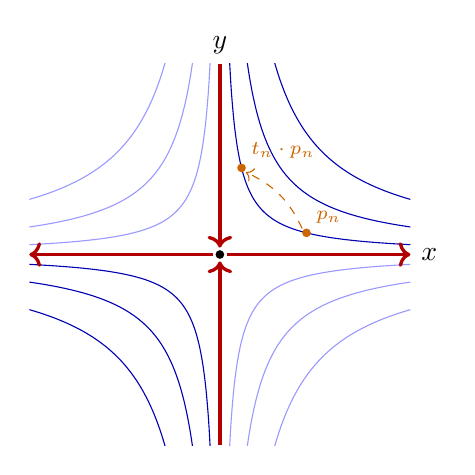
\begin{tikzpicture}[scale=1.1]
    \begin{scope}
    \clip (-2.2,-2.2) rectangle (2.2,2.2);
    \foreach \c in {0.25,0.7,1.4} {
        \draw[blue!70!black] plot[domain=0.05:2.2, samples=60, smooth] (\x, {\c/\x});
        \draw[blue!70!black] plot[domain=0.05:2.2, samples=60, smooth] (-\x, {-\c/\x});
        \draw[blue!40] plot[domain=0.05:2.2, samples=60, smooth] (\x, {-\c/\x});
        \draw[blue!40] plot[domain=0.05:2.2, samples=60, smooth] (-\x, {\c/\x});
    }
    \end{scope}
    \draw[very thick, red!70!black, ->] (0.08,0) -- (2.2,0) node[right, black] {$x$};
    \draw[very thick, red!70!black, ->] (-0.08,0) -- (-2.2,0);
    \draw[very thick, red!70!black, ->] (0,2.2) -- (0,0.08);
    \draw[very thick, red!70!black, ->] (0,-2.2) -- (0,-0.08);
    \node[above] at (0,2.2) {$y$};
    \fill (0,0) circle (0.05);
    \fill[orange!80!black] (1,0.25) circle (0.05) node[above right, font=\scriptsize] {$p_n$};
    \fill[orange!80!black] (0.25,1) circle (0.05) node[above right, font=\scriptsize] {$t_n \cdot p_n$};
    \draw[orange!80!black, dashed, ->] (0.95,0.3) to[bend right=20] (0.3,0.95);
\end{tikzpicture}
\caption{$\mathbb{R}_{>0}$ の作用 $t \cdot (x, y) = (tx, t^{-1}y)$ の軌道。青は双曲線 $xy = c$、赤は4本の開半軸（矢印は $t$ を大きくしたときの流れ）、黒点は原点。双曲線上の点 $p_n$ と $t_n \cdot p_n$ は、それぞれ $x$ 軸上と $y$ 軸上の異なる軌道に近づくので、商空間では2つの半軸の軌道が分離できない。}
\label{fig:hyperbolic}
\end{figure}


\begin{note}
点列 $p_n = (1, 1/n)$ をとると $p_n \to (1, 0)$ である。一方、$t_n = 1/n$ に対して
\begin{equation*}
    t_n \cdot p_n = \left(\frac{1}{n},\ n \cdot \frac{1}{n}\right) = \left(\frac{1}{n},\ 1\right) \to (0, 1)
\end{equation*}
となる。$p_n$ と $t_n \cdot p_n$ は同じ軌道（双曲線 $xy = 1/n$）に属するので、商空間では $[p_n]$ が $[(1,0)]$ と $[(0,1)]$ の両方に収束する。したがってこの2点は開集合で分離できない。
\end{note}

\begin{note}
ゲージ理論の $\mathcal{G} \curvearrowright \mathcal{A}$ は無限次元であるため、商多様体定理をそのまま適用することはできず、Sobolev空間による完備化が必要となる。また、$G$ の中心に値をとる定数ゲージ変換はすべての接続を固定するので、作用は決して自由ではない。そこで、中心で割った群（あるいは1点での値を $e$ に固定した基点付きゲージ群 $\mathcal{G}_0$）を用い、固定部分群が最小となる\textbf{既約接続}の空間 $\mathcal{A}^*$ に制限すると、$\mathcal{A}^*/\mathcal{G}$ は無限次元の（Banach）多様体となり、$\mathcal{A}^* \to \mathcal{A}^*/\mathcal{G}$ は主束となる。可約接続で何が起きるかは第\ref{ch:deformation}章で調べる。
\end{note}


\section{固定部分群と商空間の特異点（オービフォールド）}

物理的に興味深い多くの系では、群の作用は必ずしも自由ではない。固定部分群が自明でない点が存在すると、商空間 $M/G$ は通常の意味での滑らかな多様体とはならず、その点に特異点が生じる。本節では、固定部分群が\textbf{有限群}である場合を扱う。

典型的な状況は、離散群 $\Gamma$ が多様体 $M$ に\textbf{真性不連続}に作用している場合である。これは、任意のコンパクト集合 $K \subset M$ に対して $\{ \gamma \in \Gamma \mid \gamma K \cap K \neq \emptyset \}$ が有限集合となることをいい、離散群の作用が固有であることにほかならない。なお、「各点 $x$ が近傍 $U$ を持ち $\{ \gamma \mid \gamma U \cap U \neq \emptyset \}$ が有限」という各点ごとの条件だけでは不十分である。例えば $\mathbb{Z}$ を $\mathbb{R}^2 \setminus \{0\}$ に $(x, y) \mapsto (2x, y/2)$ で作用させると、各点ごとの条件は満たされるが、前節の双曲的スケーリングと同じ理由で $(1, 0)$ と $(0, 1)$ の軌道が分離できず、商はハウスドルフにならない。このとき各点の固定部分群 $\Gamma_x$ は有限群となる。このような商の局所的なモデルを与えるのが、次のオービフォールドの概念である。

\begin{mydef}{オービフォールド（略式）}{}
ハウスドルフ空間 $X$ が $n$ 次元の\textbf{オービフォールド}であるとは、各点 $p \in X$ が、ある有限群 $\Gamma_p \subset GL(n, \mathbb{R})$ に対する $\mathbb{R}^n / \Gamma_p$ と同相な近傍を持ち、これらの局所モデルが滑らかに貼り合わされていることをいう。$\Gamma_p \neq \{e\}$ である点を\textbf{オービフォールド特異点}、$\Gamma_p$ をその\textbf{局所群}と呼ぶ。
\end{mydef}

\begin{mythm}{有限な固定部分群を持つ商}{orbifold}
離散群 $\Gamma$ が $n$ 次元多様体 $M$ に滑らかかつ真性不連続に作用しているとする。このとき $M/\Gamma$ はオービフォールドであり、点 $[x]$ の局所群は固定部分群 $\Gamma_x$（$x$ における接空間 $T_x M \cong \mathbb{R}^n$ への線形作用）で与えられる。特に、$\Gamma_x = \{e\}$ となる点の近傍では $M/\Gamma$ は滑らかな多様体である。
\end{mythm}

より一般に、リー群 $G$ が固有に作用する場合も\textbf{スライス定理}により、軌道 $G \cdot x$ の近傍で $M/G$ は局所的に $S/G_x$（$S$ は軌道に横断的なスライス）と表される。$G_x$ が有限群ならオービフォールド特異点、連続群なら錐のようなより深刻な特異点が現れる（後者は第\ref{ch:deformation}章で扱う）。

\paragraph{例：錐 $\mathbb{C}/\mathbb{Z}_n$}
$\zeta = e^{2\pi i/n}$ とし、$\mathbb{Z}_n = \{ \zeta^k \}$ を $z \mapsto \zeta z$ によって $\mathbb{C}$ に作用させる。固定点は原点のみで、$\Gamma_0 = \mathbb{Z}_n$、それ以外の点の固定部分群は自明である。基本領域として扇形 $0 \le \arg z < 2\pi/n$ をとり、その2辺を貼り合わせると、商は頂角 $2\pi/n$ の\textbf{円錐}となる（図\ref{fig:cone}）。

\begin{figure}[htbp]
\centering
\begin{tikzpicture}
    % 左：扇形
    \begin{scope}
        \fill[blue!10] (0,0) -- (2,0) arc (0:120:2) -- cycle;
        \draw[gray, dashed] (0,0) circle (2);
        \draw[very thick, red!70!black] (0,0) -- (2,0);
        \draw[very thick, red!70!black] (0,0) -- (120:2);
        \draw[->, red!70!black] (1.5,0.05) to[bend right=50] node[right, font=\scriptsize] {$z \mapsto \zeta z$} (120:1.5);
        \fill (0,0) circle (0.05) node[below] {$0$};
        \node at (50:0.85) {基本領域};
        \node[font=\scriptsize] at (0,-2.4) {$0 \le \arg z \le 2\pi/n$（図は $n = 3$）};
    \end{scope}
    \draw[->, thick] (2.6,0) -- node[above] {貼り合わせ} (3.8,0);
    % 右：錐
    \begin{scope}[xshift=5.5cm]
        \draw[thick] (0,1.6) -- (-1.2,-1.0);
        \draw[thick] (0,1.6) -- (1.2,-1.0);
        \draw[thick] (-1.2,-1.0) arc (180:360:1.2 and 0.35);
        \draw[thick, dashed] (1.2,-1.0) arc (0:180:1.2 and 0.35);
        \draw[very thick, red!70!black] (0,1.6) -- (0.3,-1.33);
        \fill (0,1.6) circle (0.05) node[above] {頂点（$\Gamma_0 = \mathbb{Z}_n$）};
        \node[font=\scriptsize] at (0,-2.0) {頂角 $2\pi/n$ の円錐};
    \end{scope}
\end{tikzpicture}
\caption{錐 $\mathbb{C}/\mathbb{Z}_n$ の作り方。扇形の基本領域の2辺（赤）を貼り合わせると、原点が頂点となる円錐ができる。頂点のまわりを1周したときの角度は $2\pi/n$ しかない。}
\label{fig:cone}
\end{figure}

興味深いのは、位相空間としては $w = z^n$ によって $\mathbb{C}/\mathbb{Z}_n \cong \mathbb{C}$ と同相であり、特異点が見えないことである。しかし平坦な計量 $|dz|^2$ を商に降ろすと、原点のまわりを1周したときの角度が $2\pi$ ではなく $2\pi/n$ となり、原点に曲率が集中した円錐特異点となる。オービフォールドの構造（局所群 $\mathbb{Z}_n$）は、位相だけでは見えないこの情報を記憶している。

\paragraph{例：トーラスのモジュライ空間}
第\ref{ch:intro}章のトーラスのモジュライ $\mathcal{M}_1 = \mathbb{H}/SL(2, \mathbb{Z})$ を考えよう。$-1 \in SL(2,\mathbb{Z})$ は $\tau \mapsto \tau$ と自明に作用するので、実効的に作用するのは $PSL(2, \mathbb{Z}) = SL(2, \mathbb{Z})/\{\pm 1\}$ であり、これは
\begin{equation}
    S: \tau \mapsto -\frac{1}{\tau}, \qquad T: \tau \mapsto \tau + 1
\end{equation}
で生成され、$\mathbb{H}$ に真性不連続に作用する。固定部分群を計算すると、$\tau = i$ では $\mathbb{Z}_2 = \langle S \rangle$、$\tau = e^{i\pi/3}$（およびそれと同じ軌道の $e^{2\pi i/3}$）では $\mathbb{Z}_3$ であり、それ以外の点（基本領域の内部）では自明である。

\begin{note}
$\tau = i$：$S(i) = -1/i = i$ であり、$PSL(2, \mathbb{Z})$ において $S^2 = 1$ なので、固定部分群は $\langle S \rangle \cong \mathbb{Z}_2$。

$\tau = \omega = e^{2\pi i/3}$：$1 + \omega + \omega^2 = 0$ より $\omega + 1 = -\omega^2$ なので、
\begin{equation*}
    ST(\omega) = S(\omega + 1) = -\frac{1}{\omega + 1} = \frac{1}{\omega^2} = \omega
\end{equation*}
である。$(ST)^3 = 1$ より固定部分群は $\langle ST \rangle \cong \mathbb{Z}_3$。$e^{i\pi/3} = \omega + 1 = T(\omega)$ は $\omega$ と同じ軌道に属するので、その固定部分群は共役な $T \langle ST \rangle T^{-1} \cong \mathbb{Z}_3$ である（軌道・固定部分群定理の (3)）。

$SL(2, \mathbb{Z})$ の中で数えれば、$-1$ を含めてそれぞれ位数4と位数6の巡回群となる。
\end{note}

したがって定理より、$\mathcal{M}_1$ は $\tau = i$ に頂角 $\pi$、$\tau = e^{i\pi/3}$ に頂角 $2\pi/3$ の円錐特異点を持つオービフォールドである。これは基本領域 $\{|\tau| \ge 1,\ |\mathrm{Re}\,\tau| \le 1/2\}$ の境界を貼り合わせたときに、$\tau = i$ では円弧が折り返されて角度 $\pi$、2つの角 $e^{i\pi/3}, e^{2\pi i/3}$（それぞれ内角 $\pi/3$）が貼り合わされて角度 $2\pi/3$ となることと一致している。

\paragraph{例：$T^2/\mathbb{Z}_2$（枕カバー）}
トーラス $T^2 = \mathbb{C}/(\mathbb{Z} + \tau\mathbb{Z})$ に $\mathbb{Z}_2$ を $z \mapsto -z$ で作用させる。固定点は $-z \equiv z$、すなわち $2z \in \mathbb{Z} + \tau\mathbb{Z}$ を満たす点であり、
\begin{equation}
    z = 0,\quad \frac{1}{2},\quad \frac{\tau}{2},\quad \frac{1 + \tau}{2}
\end{equation}
の4点である。それぞれ局所群 $\mathbb{Z}_2$（頂角 $\pi$ の円錐点）を持ち、商は位相的には球面 $S^2$ で、平坦な計量を持つ「4つの角を持つ枕」の形をしている。

\begin{note}
この結果の整合性をGauss--Bonnetの定理で確かめよう。平坦な曲面の全曲率は円錐点の角度欠損 $2\pi - (\text{頂角})$ の和で与えられ、
\begin{equation*}
    \sum_{\text{円錐点}} (2\pi - \pi) = 4\pi = 2\pi \chi(S^2)
\end{equation*}
となって、確かに球面のEuler数 $\chi = 2$ と一致する。

より一般に、オービフォールドには\textbf{オービフォールドEuler数}
\begin{equation*}
    \chi^{\mathrm{orb}}(X) = \chi(X) - \sum_{p} \left( 1 - \frac{1}{|\Gamma_p|} \right)
\end{equation*}
が定義され、有限群 $\Gamma$ による商では $\chi^{\mathrm{orb}}(M/\Gamma) = \chi(M)/|\Gamma|$ が成り立つ。枕カバーでは $2 - 4 \cdot \frac{1}{2} = 0 = \chi(T^2)/2$ である。トーラスのモジュライ空間に適用すると、カスプを除いた下部空間は $\mathbb{C}$（$\chi = 1$）なので
\begin{equation*}
    \chi^{\mathrm{orb}}(\mathbb{H}/PSL(2,\mathbb{Z})) = 1 - \left(1 - \frac{1}{2}\right) - \left(1 - \frac{1}{3}\right) = -\frac{1}{6}
\end{equation*}
となり、すべての点に共通する自己同型 $-1$（$z \mapsto -z$）も数えると $\chi^{\mathrm{orb}}(\mathcal{M}_{1,1}) = -\frac{1}{12} = \zeta(-1)$ を得る（Harer--Zagier\cite{harerzagier1986}）。
\end{note}

\begin{note}
超弦理論の余剰次元のコンパクト化において、このオービフォールド特異点は極めて重要な物理的役割を果たす。時空を有限群の作用で割ったオービフォールド（例えば $T^2/\mathbb{Z}_2$ や $\mathbb{C}^2/\mathbb{Z}_2$）を考えると、固定点のまわりを回る閉弦の境界条件として「ねじれたセクター（twisted sector）」が許容される。これにより、特異点上に質量ゼロの新しい粒子が局所的に出現し、低エネルギーでのゲージ対称性の拡大や対称性の破れなどを決定づける。このような特異点を含む空間上の幾何学や場の理論を矛盾なく扱うための強力な枠組みが、後の章で扱う「モジュライスタック」である。
\end{note}


\section{大域的な障害：Gribov問題と大域的定義の困難}

前節までは局所的な特異点の問題であったが、商空間を構成する際には大域的なトポロジーの障害も立ちはだかる。局所的なゲージ固定条件を導入してモジュライ空間 $\mathcal{A}/\mathcal{G}$ を構成しようとするとき、数学的に深刻な大域的障害に直面することがある。これが\textbf{Gribov問題（Gribov ambiguity）}である\cite{gribov1978}。

写像 $F: \mathcal{A} \to V$（$V$ はベクトル空間）による条件 $F(A) = 0$ を\textbf{ゲージ固定条件}という。理想的には、零点集合 $F^{-1}(0)$ が各ゲージ軌道とちょうど1点で横断的に交わり、各軌道 $[A]$ にその交点を対応させる写像 $s: \mathcal{A}/\mathcal{G} \to \mathcal{A}$ が連続になることが望ましい。このような $s$（$\pi \circ s = \mathrm{id}$ を満たす連続写像）は、主束 $\pi: \mathcal{A} \to \mathcal{A}/\mathcal{G}$ の\textbf{大域的切断}に他ならない。これに対し、同一のゲージ軌道上の異なる2点 $A \neq A^U$ がともにゲージ固定条件を満たすとき、これらを互いの\textbf{Gribovコピー}と呼ぶ。

\paragraph{例：有限次元の玩具模型}
$SO(2)$ を回転によって $\mathbb{R}^2 \setminus \{0\}$ に作用させる。軌道は原点を中心とする円周であり、商は動径 $r > 0$ で完全に記述される。ここに「ゲージ固定条件」$F(x, y) = y = 0$ を課すと、半径 $r$ の軌道は $y = 0$ と $(r, 0)$、$(-r, 0)$ の\textbf{2点}で交わり、これらは互いにGribovコピーとなる。さらに、2つのコピーではFaddeev--Popov行列式の符号が逆になり、絶対値をとらずにFaddeev--Popovの処方を適用すると、「軌道の体積で割る」ための規格化因子がちょうどゼロになってしまう。条件 $\Delta_{\mathrm{FP}} > 0$（すなわち $x > 0$）に制限すれば、各軌道との交点はちょうど1つになる。これが\textbf{Gribov領域}への制限の玩具版である。

\begin{note}
点 $(r, 0)$ を角度 $\theta$ だけ回転させると $F(\theta) = r\sin\theta$ であり、その零点は $\theta = 0, \pi$ である。Faddeev--Popov行列式（今は $1 \times 1$）は
\begin{equation*}
    \Delta_{\mathrm{FP}} = \left.\frac{\partial F}{\partial \theta}\right|_{\text{零点}} = r\cos\theta = \begin{cases} +r & (\theta = 0) \\ -r & (\theta = \pi) \end{cases}
\end{equation*}
となる。絶対値をとらずにFaddeev--Popovの恒等式を用いると
\begin{equation*}
    \int_0^{2\pi} d\theta\, \delta(F(\theta))\, \frac{\partial F}{\partial \theta} = \sum_{\text{零点}} \mathrm{sign}\left(\frac{\partial F}{\partial \theta}\right) = (+1) + (-1) = 0
\end{equation*}
となり、規格化因子が消える。一方、$x > 0$ に制限すれば零点は $\theta = 0$ のみとなり、値は $1$ に戻る。
\end{note}

\paragraph{例：Coulombゲージの無限小Gribovコピー}
Coulomb（Landau）ゲージ $\partial^\mu A_\mu = 0$ を考える。$A$ に無限小ゲージ変換を施したものが再びゲージ条件を満たすための条件は、Faddeev--Popov演算子
\begin{equation}
    \mathcal{M}_{\mathrm{FP}} = -\partial^\mu D_\mu, \qquad D_\mu \epsilon \equiv \partial_\mu \epsilon - ig[A_\mu, \epsilon]
\end{equation}
が零モードを持つことと同値である。可換な場合（$U(1)$）は $\mathcal{M}_{\mathrm{FP}} = -\partial^2$ であり、無限遠で減衰する零モードは存在しないので、無限小のGribovコピーはない。一方、非可換な場合は $A$ に依存する項のため、$A$ が十分大きくなると $\mathcal{M}_{\mathrm{FP}}$ の最低固有値がゼロに達し、無限小のGribovコピーが現れる。$\mathcal{M}_{\mathrm{FP}}$ が初めて零モードを持つ境界を\textbf{Gribov地平線}、その内側 $\Omega = \{ A \mid \partial \cdot A = 0,\ \mathcal{M}_{\mathrm{FP}} > 0 \}$ を\textbf{Gribov領域}と呼ぶ。

\begin{note}
無限小ゲージ変換 $U = e^{ig\epsilon} \simeq 1 + ig\epsilon$ を式 \eqref{eq:gauge-transf-ch2} に代入すると、
\begin{align*}
    U A_\mu U^{-1} &\simeq A_\mu + ig[\epsilon, A_\mu], \\
    -\frac{i}{g}(\partial_\mu U) U^{-1} &\simeq -\frac{i}{g}(ig\,\partial_\mu \epsilon) = \partial_\mu \epsilon
\end{align*}
より
\begin{equation*}
    \delta A_\mu = \partial_\mu \epsilon + ig[\epsilon, A_\mu] = \partial_\mu \epsilon - ig[A_\mu, \epsilon] = D_\mu \epsilon
\end{equation*}
を得る。$\partial^\mu A_\mu = 0$ を満たす $A$ に対して、変換後も $\partial^\mu (A_\mu + \delta A_\mu) = 0$ となる条件は $\partial^\mu D_\mu \epsilon = 0$、すなわち $\mathcal{M}_{\mathrm{FP}}\, \epsilon = 0$ である。
\end{note}

玩具模型ではGribov領域への制限によって問題が解消したが、次の定理\cite{singer1978}は、非可換ゲージ理論ではそもそも大域的切断が存在しないことを示している。

\begin{mythm}{Singer, 1978}{}
$M = S^4$（あるいは $S^3$）、$G = SU(N)$（$N \ge 2$）とする。既約接続の空間 $\mathcal{A}^*$ と基点付きゲージ群 $\mathcal{G}_0$ に対し、主束 $\mathcal{A}^* \to \mathcal{A}^*/\mathcal{G}_0$ は自明ではない。特に、連続な大域的ゲージ固定（大域的切断）は存在しない。
\end{mythm}
\begin{proof}[証明の概略]
主束が自明ならば $\mathcal{A}^* \simeq (\mathcal{A}^*/\mathcal{G}_0) \times \mathcal{G}_0$ であり、$\mathcal{G}_0$ のホモトピー群は $\mathcal{A}^*$ のホモトピー群の直和因子となる。$\mathcal{A}$ はアフィン空間（可縮）であり、$\mathcal{A}^*$ はそこから「無限余次元」の部分集合を除いたものなので、すべてのホモトピー群が自明である。一方、$S^4$ 上の基点付きゲージ群は $\pi_k(\mathcal{G}_0) \cong \pi_{k+4}(G)$ を満たし、例えば $G = SU(2) \cong S^3$ に対して
\begin{equation*}
    \pi_1(\mathcal{G}_0) \cong \pi_5(S^3) \cong \mathbb{Z}_2 \neq 0
\end{equation*}
である。これは矛盾である。
\end{proof}

\begin{note}
証明で用いた事実（直積のホモトピー群 $\pi_k(X \times Y) \cong \pi_k(X) \times \pi_k(Y)$、可縮な空間のホモトピー群は自明、$\pi_k(\mathcal{G}_0) \cong \pi_{k+4}(G)$、$\pi_5(S^3) \cong \mathbb{Z}_2$）は付録\ref{sec:topo-pin}節にまとめた。$\mathcal{A}^*$ について「無限余次元の部分集合を除いてもホモトピー群は自明のまま」なのは、有限次元の球面の像を、無限余次元の部分集合（可約接続の集合）を避けるように動かせるからである（$\mathbb{R}^3$ 内のループが1点を避けられるのと同じ理屈）。
\end{note}

\begin{note}
Gribovコピーの存在は、Faddeev--Popovの処方が摂動論的な枠組み（微小なゲージ変換の範囲）でのみ有効であり、非摂動領域では破綻することを示唆している。経路積分においてGribov領域に積分を制限する試み（Gribov--Zwanzigerの処方）などが行われているが、Singerの定理が示すように、モジュライ空間は単純な商空間 $M/G$ として一つの座標系で大域的に書き表すことができない。このことは、複数のパッチによる貼り合わせの構造や、スタックとしての定式化が必要であることを数学的に意味している。
\end{note}

\section{まとめと次章への展望}

本章では、物理的冗長性としてのゲージ対称性を割り引き、真の自由度を抽出する操作が「群作用による商空間の構成」に他ならないことを見た。群作用の性質と商空間の性質の対応は、次のようにまとめられる。
\begin{itemize}
    \item \textbf{自由かつ固有}な作用 $\Rightarrow$ $M/G$ は滑らかな多様体で、$M \to M/G$ は主 $G$ 束（定理 \ref{thm:quotient-manifold}）。
    \item 固有で、固定部分群が\textbf{有限群} $\Rightarrow$ $M/G$ はオービフォールド（定理 \ref{thm:orbifold}。錐やトーラスのモジュライ空間）。
    \item 固定部分群が\textbf{連続群} $\Rightarrow$ 境界や錐のような、より深刻な特異点（平面の回転の例、第\ref{ch:deformation}章）。
    \item \textbf{固有でない}作用 $\Rightarrow$ $M/G$ はハウスドルフ性を失いうる（無理数回転、双曲的スケーリング、第\ref{ch:vacuum}章のGIT商）。
    \item 局所的には良い商でも、\textbf{大域的切断が存在しない}ことがある $\Rightarrow$ Gribov問題（Singerの定理）。
\end{itemize}

次章では、モジュライ空間の局所的な形状や次元を決定づける\textbf{接空間・特異点・次元}の解析手法、およびそれを変形理論とコホモロジー群の言葉でどのように定式化するかについて詳しく見ていく。
\chapter{接空間・特異点・次元：モジュライの自由度を理解する}
\label{ch:deformation}

モジュライ空間の大域的な構造（トポロジーや特異点）を完全に理解することは一般に困難であるが、ある解の近傍における局所的な構造は、線形化された方程式とコホモロジー理論を用いて系統的に調べることができる。本章では、モジュライ空間の接空間がどのように定義され、物理的な「零モード（ゼロ・モード）」とどのように対応するのかを、ゲージ理論および複素幾何学の変形理論（小平・スペンサー理論）を題材に詳細に解説する。

\section{零モードと集団座標：接空間はなぜ物理的に重要か}

経路積分において、ある古典解 $\phi_{\text{cl}}$ のまわりでの半古典近似を考えよう。場を $\phi = \phi_{\text{cl}} + \delta\phi$ と分けて作用を展開すると、古典解は停留点であるから1次の項は消え、
\begin{equation}
    S[\phi_{\text{cl}} + \delta\phi] = S[\phi_{\text{cl}}] + \frac{1}{2}\int d^dx\, \delta\phi\, \Delta\, \delta\phi + \mathcal{O}(\delta\phi^3)
\end{equation}
となる。ここで $\Delta = \left.\frac{\delta^2 S}{\delta\phi\,\delta\phi}\right|_{\phi_{\text{cl}}}$ は2次の揺らぎ演算子（Hessian）である。$\Delta$ の固有値がすべて正であれば、Gauss積分により
\begin{equation}
    Z \simeq e^{-S[\phi_{\text{cl}}]} \left(\det \Delta\right)^{-1/2}
\end{equation}
を得る。

しかし、古典解が連続族 $\phi_{\text{cl}}(x; m^1, \dots, m^n)$ をなす場合、パラメータ $m^i$ に関する微分
\begin{equation}
    \delta_i \phi \equiv \frac{\partial \phi_{\text{cl}}}{\partial m^i}
\end{equation}
は $\Delta\,\delta_i\phi = 0$ を満たす固有値ゼロの固有関数、すなわち\textbf{零モード}となる。

\begin{note}
すべての $m$ に対して運動方程式 $\left.\frac{\delta S}{\delta \phi}\right|_{\phi_{\text{cl}}(m)} = 0$ が成り立つ。これを $m^i$ で微分すると
\begin{equation}
    0 = \frac{\partial}{\partial m^i}\left.\frac{\delta S}{\delta \phi(x)}\right|_{\phi_{\text{cl}}(m)} = \int d^dy\, \left.\frac{\delta^2 S}{\delta \phi(x)\delta\phi(y)}\right|_{\phi_{\text{cl}}} \frac{\partial \phi_{\text{cl}}(y)}{\partial m^i} = (\Delta\, \delta_i\phi)(x)
\end{equation}
となり、$\delta_i\phi$ が零モードであることが分かる。逆に言えば、零モードとは「線形化された運動方程式の解」であり、これはまさに解の空間の接ベクトルである。
\end{note}

零モード方向では作用が変化しないため、その方向のGauss積分は発散し、$(\det\Delta)^{-1/2}$ は意味を失う。正しい処方は、零モード方向の積分をモジュライ・パラメータ（\textbf{集団座標（collective coordinates）}）$m^i$ の積分に置き換えることである。
\begin{equation}
    Z \simeq \int_{\mathcal{M}} \prod_{i=1}^{n} \frac{dm^i}{\sqrt{2\pi}}\, \sqrt{\det g_{ij}(m)}\; e^{-S[\phi_{\text{cl}}]} \left({\det}' \Delta\right)^{-1/2}
\end{equation}
ここで ${\det}'$ は零固有値を除いた行列式であり、
\begin{equation}
    g_{ij}(m) = \int d^dx\, \delta_i\phi\, \delta_j\phi
\end{equation}
は零モードの内積から定まるモジュライ空間上の自然な計量（変数変換のJacobian）である。

このように、半古典的な経路積分は「モジュライ空間 $\mathcal{M}$ 上の有限次元積分」に帰着する。したがって次の対応がある。
\begin{itemize}
    \item モジュライ空間の\textbf{次元}は、零モード（集団座標）の数を与える。
    \item モジュライ空間の\textbf{計量}は、集団座標の積分測度を与える。
    \item モジュライ空間の\textbf{特異点や非コンパクト性}は、積分の発散や境界からの寄与として物理に現れる。
\end{itemize}
ただしゲージ理論では、ゲージ変換によって生成される $\Delta$ の零固有値（ゲージ零モード）は物理的な零モードではなく、ゲージ固定によって除去しなければならない。この「物理的零モード」と「ゲージ零モード」の分離を正確に行う道具が、以下で導入する変形複体とそのコホモロジーである。

\section{ゲージ接続のモジュライと楕円型複体}

多様体 $M$ 上の主 $G$ 束 $P$ におけるゲージ接続の空間 $\mathcal{A}$ を考え、ゲージ群 $\mathcal{G}$ の作用による商空間としてモジュライ空間 $\mathcal{M} = \mathcal{A}/\mathcal{G}$ を定義した。ある特定の接続 $A \in \mathcal{A}$ が与えられたとき、モジュライ空間上の点 $[A] \in \mathcal{M}$ における接空間 $T_{[A]}\mathcal{M}$ はどのように記述されるだろうか。

接ベクトルとは、「物理的に等価でない無限小変形」のことである。接続の微小変形 $A \to A + \delta A$ を考える。接続空間 $\mathcal{A}$ はアフィン空間であるため、二つの接続の差 $\delta A$ は $M$ 上の $\mathrm{ad}(P)$ に値をとる1次微分形式（$\delta A \in \Omega^1(M, \mathrm{ad}(P))$）となる。

ここで、我々が興味を持つのは、運動方程式（例えば反自己双対方程式 $F^+ = 0$ や平坦接続 $F = 0$）を満たす解のモジュライである。簡単のため、平坦接続のモジュライを例にとる。

\begin{note}
平坦条件 $F(A) = 0$ が変形後も保たれる条件を導出する。
曲率の定義 $F(A) = dA + A \wedge A$ に対し、$A \to A + \delta A$ を代入すると、
\begin{align*}
F(A + \delta A) &= d(A + \delta A) + (A + \delta A) \wedge (A + \delta A) \\
&= dA + d(\delta A) + A \wedge A + A \wedge \delta A + \delta A \wedge A + \delta A \wedge \delta A \\
&= F(A) + d(\delta A) + [A, \delta A] + \mathcal{O}(\delta A^2)
\end{align*}
となる。ここで、リー代数に値をとる微分形式の交換子関係 $[\alpha, \beta] = \alpha \wedge \beta - (-1)^{|\alpha||\beta|} \beta \wedge \alpha$ を用いた。
バックグラウンドが $F(A) = 0$ を満たすとし、無限小変形の一次のオーダーを取り出すと、
\begin{equation}
    d_A (\delta A) \equiv d(\delta A) + [A, \delta A] = 0
\end{equation}
が得られる。すなわち、変形 $\delta A$ は共変外微分 $d_A: \Omega^1 \to \Omega^2$ の核（kernel）に属さなければならない。
\end{note}

しかし、方程式 $d_A(\delta A) = 0$ を満たす変形の中には、単なるゲージ変換による物理的に自明な変形が含まれている。無限小ゲージパラメータ $\epsilon \in \Omega^0(M, \mathrm{ad}(P))$ による変換を考えよう。

\begin{note}
有限ゲージ変換は $A \to A^U = U^{-1} A U + U^{-1} d U$ で与えられる（本講義の規約に合わせる）。
$U = e^\epsilon \simeq 1 + \epsilon$ と展開すると、
\begin{align*}
A^{1+\epsilon} &= (1 - \epsilon) A (1 + \epsilon) + (1 - \epsilon) d(1 + \epsilon) + \mathcal{O}(\epsilon^2) \\
&= A - \epsilon A + A \epsilon + d\epsilon + \mathcal{O}(\epsilon^2) \\
&= A + d\epsilon + [A, \epsilon] = A + d_A \epsilon
\end{align*}
したがって、ゲージ変換による純粋な冗長性は $\delta_{gauge} A = d_A \epsilon$ と書ける。これは共変外微分 $d_A: \Omega^0 \to \Omega^1$ の像（image）である。
\end{note}

以上より、真の物理的自由度（モジュライ空間の接空間）は、「線形化された方程式を満たす変形」を「ゲージ変換による冗長性」で割った空間として与えられる。これを定理の形でまとめておこう。

\begin{mythm}{平坦接続のモジュライの接空間}{flat-tangent}
$A$ を平坦接続とし、平坦接続のモジュライ空間 $\mathcal{M}$ が点 $[A]$ の近傍で滑らかであるとする。このとき
\begin{equation*}
    T_{[A]}\mathcal{M} \cong H^1(M, d_A) = \frac{\ker (d_A: \Omega^1 \to \Omega^2)}{\mathrm{im} (d_A: \Omega^0 \to \Omega^1)}
\end{equation*}
が成り立つ。（滑らかであるための十分条件は、\ref{sec:higher-cohomology}節で見るように $H^0 = H^2 = 0$ である。）
\end{mythm}

このコホモロジーの各元が、経路積分における「ゲージ不変な零モード」に1対1対応する。

\subsection{変形複体とHodge理論によるゲージ固定}

上の構成は、次の微分形式の系列としてまとめることができる。
\begin{equation}
    0 \longrightarrow \Omega^0(M, \mathrm{ad}P) \xrightarrow{\ d_A\ } \Omega^1(M, \mathrm{ad}P) \xrightarrow{\ d_A\ } \Omega^2(M, \mathrm{ad}P) \xrightarrow{\ d_A\ } \cdots
\end{equation}
左の矢印は無限小ゲージ変換、右の矢印は線形化された平坦条件を表す。

\begin{mydef}{変形複体とそのコホモロジー}{}
平坦接続 $A$ に対し、上の系列を $A$ の\textbf{変形複体}と呼び、そのコホモロジー
\begin{equation*}
    H^i(M, d_A) = \frac{\ker (d_A: \Omega^i(M, \mathrm{ad}P) \to \Omega^{i+1}(M, \mathrm{ad}P))}{\mathrm{im} (d_A: \Omega^{i-1}(M, \mathrm{ad}P) \to \Omega^{i}(M, \mathrm{ad}P))}
\end{equation*}
を定める（$\Omega^{-1} = 0$ とする）。$H^0$ は\textbf{無限小自己同型}、$H^1$ は\textbf{無限小変形}、$H^2$ は\textbf{変形の障害}の空間と解釈される（\ref{sec:higher-cohomology}節）。
\end{mydef}

これが複体（$d_A \circ d_A = 0$）をなすことは、背景が平坦であることと同値である。

\begin{note}
$\epsilon \in \Omega^0(M, \mathrm{ad}P)$ に $d_A$ を2回作用させる。$A$ が1次形式であることに注意して $d[A, \epsilon] = [dA, \epsilon] - [A, d\epsilon]$ を用いると、
\begin{align*}
d_A d_A \epsilon &= d(d\epsilon + [A, \epsilon]) + [A, d\epsilon + [A, \epsilon]] \\
&= [dA, \epsilon] - [A, d\epsilon] + [A, d\epsilon] + [A, [A, \epsilon]] \\
&= [dA, \epsilon] + [A \wedge A, \epsilon] = [F, \epsilon]
\end{align*}
ここで次数付きJacobi恒等式より $[A, [A, \epsilon]] = \frac{1}{2}[[A, A], \epsilon] = [A \wedge A, \epsilon]$ を用いた。したがって $d_A^2 = [F, \cdot\,]$ であり、$F = 0$ のときに限り複体となる。一般の $p$ 形式に対しても同様に $d_A^2 \alpha = [F, \alpha]$ が成り立つ。
\end{note}

商空間 $\ker d_A / \mathrm{im}\, d_A$ を具体的に扱うには、各同値類から代表元を1つ選ぶ（ゲージ固定する）必要がある。$M$ 上にRiemann計量を、$\mathrm{ad}P$ 上に不変内積（例えば $-\mathrm{Tr}$）を入れ、$d_A$ の形式的随伴 $d_A^*$ を定義しよう。変形 $\delta A$ がゲージ軌道に直交するという条件
\begin{equation}
    \langle d_A \epsilon, \delta A \rangle = \langle \epsilon, d_A^* \delta A \rangle = 0 \quad (\forall \epsilon) \iff d_A^* \delta A = 0
\end{equation}
は、背景場Lorenzゲージ $D^\mu \delta A_\mu = 0$ に他ならない。これを線形化方程式と組み合わせた
\begin{equation}
    d_A \delta A = 0, \qquad d_A^* \delta A = 0
\end{equation}
は楕円型の連立方程式である。楕円型作用素に対する一般論から、次が成り立つ。

\begin{mythm}{Hodge分解と有限次元性}{hodge}
$M$ をコンパクトなRiemann多様体、$A$ を平坦接続とする。このとき
\begin{enumerate}
    \item 各コホモロジー類はただ1つの調和代表元を持つ：
    \begin{equation*}
        H^1(M, d_A) \cong \mathcal{H}^1_A \equiv \{ \delta A \in \Omega^1(M, \mathrm{ad}P) \mid d_A \delta A = d_A^* \delta A = 0 \}
    \end{equation*}
    \item $\mathcal{H}^1_A$（したがって $H^1(M, d_A)$）は\textbf{有限次元}である。
\end{enumerate}
\end{mythm}無限次元の空間 $\mathcal{A}$ を無限次元の群 $\mathcal{G}$ で割ったにもかかわらずモジュライ空間が有限次元となるのは、このためである。

\begin{note}
物理的には、ゲージ直交条件 $d_A^*\delta A = 0$ を課した零モードが「物理的零モード」であり、$\mathrm{im}\,d_A$ に属する零モードは前節で述べた「ゲージ零モード」である。Hodge分解
\begin{equation}
    \Omega^1(M, \mathrm{ad}P) = \mathrm{im}\, d_A \oplus \mathcal{H}^1_A \oplus \mathrm{im}\, d_A^*
\end{equation}
において、第1項がゲージ方向、第2項がモジュライ方向、第3項が作用を実際に増加させる（質量を持つ）揺らぎに対応する。前節の計量 $g_{ij}$ は、ゲージ固定された零モードの $L^2$ 内積
\begin{equation}
    g(\delta_1 A, \delta_2 A) = -\int_M \mathrm{Tr}(\delta_1 A \wedge * \delta_2 A)
\end{equation}
として与えられる。
\end{note}

\subsection{例：トーラス上の平坦 $U(1)$ 接続とWilsonライン}

最も簡単な例として、$n$ 次元トーラス $T^n$（座標 $x^i \sim x^i + 2\pi$）上の $U(1)$ 平坦接続を考える。$U(1)$ の場合 $A = i a$（$a$ は実1次形式）と書けて交換子は消えるので、$d_A = d$ であり、変形複体はde Rham複体そのものになる。したがって
\begin{equation}
    T_{[A]}\mathcal{M} \cong H^1_{\mathrm{dR}}(T^n) \cong \mathbb{R}^n
\end{equation}
であり、調和代表元は定数係数の1次形式 $a = \theta_i\, dx^i$ である。各サイクルに沿ったホロノミー（Wilsonライン）は
\begin{equation}
    W_i = \exp\left( i \oint_{S^1_i} a \right) = e^{2\pi i \theta_i}
\end{equation}
で与えられる。

ここで、$U = e^{i m_i x^i}$（$m_i \in \mathbb{Z}$）というゲージ変換を考えると、これは $T^n$ 上で一価な関数であるから正当なゲージ変換であり、$a \to a + m_i\, dx^i$、すなわち $\theta_i \to \theta_i + m_i$ を引き起こす。よって $\theta_i$ は周期 $1$ で同一視され、
\begin{equation}
    \mathcal{M}_{\text{flat}}(T^n, U(1)) \cong \mathbb{R}^n / \mathbb{Z}^n \cong T^n
\end{equation}
を得る。一般に平坦接続はホロノミーで完全に決まるので、$\mathcal{M}_{\text{flat}}(M, G) \cong \mathrm{Hom}(\pi_1(M), G)/G$ が成り立つ。

\begin{note}
$H^1_{\mathrm{dR}}(T^n) \cong \mathbb{R}^n$（基底 $dx^i$ は閉形式だが、$\oint_{S^1_i} dx^i = 2\pi \neq 0$ なので完全形式でない）の証明と、Betti数 $b_k = \dim H^k_{\mathrm{dR}}$ については付録\ref{sec:topo-derham}節を参照。

\textbf{$\mathcal{M}_{\text{flat}} \cong \mathrm{Hom}(\pi_1(M), G)/G$ について。}
平坦接続のホロノミーはループを連続変形しても変わらない（第\ref{ch:bundle}章）ので、基点 $x_0$ を通るループの類 $[\gamma] \in \pi_1(M, x_0)$（付録\ref{sec:topo-pi1}節）ごとに元 $\mathrm{Hol}(\gamma) \in G$ が定まる。ループをつなぐとホロノミーは掛け算になるので、これは群の準同型 $\pi_1(M) \to G$ である。基点 $x_0$ でのゲージ変換 $g$ はすべてのホロノミーを同時に共役 $\mathrm{Hol} \mapsto g\,\mathrm{Hol}\,g^{-1}$ で変えるので、ゲージ同値類は準同型の共役類に対応する。逆に、準同型が与えられれば、普遍被覆の上の自明な接続を「ループに沿って回るとホロノミーだけずれる」ように貼り合わせて、平坦接続を再構成できる。トーラスの場合は $\pi_1(T^n) \cong \mathbb{Z}^n$ であり、準同型 $\mathbb{Z}^n \to U(1)$ は各生成元の行き先 $W_i = e^{2\pi i \theta_i}$ で決まる。$U(1)$ は可換なので共役は自明であり、$\mathrm{Hom}(\mathbb{Z}^n, U(1)) = U(1)^n = T^n$ は本文の結果と一致する。
\end{note}

\begin{note}
この例は、モジュライ空間の局所構造（$H^1 \cong \mathbb{R}^n$）と大域構造（$T^n$）の違いをよく示している。接空間の計算は無限小のゲージ変換 $\mathrm{im}\, d$ による商しか見ないが、大域的には巻き付き数を持つ「大きなゲージ変換」による同一視が加わり、モジュライ空間はコンパクトなトーラスになる。弦理論では、コンパクト化された方向に沿ったWilsonライン $\theta_i$ は低エネルギーでスカラー場（モジュライ場）として振る舞い、T双対性のもとでDブレーンの位置座標に移る。モジュライ空間として「双対トーラス」が現れるのはこのためである。
\end{note}

\section{複素幾何における変形理論（小平・スペンサー理論）}

モジュライ空間の接空間をコホモロジーで捉える枠組みは、ゲージ理論に限らず、弦理論における余剰次元（Calabi--Yau多様体など）の分類でも中心的な役割を果たす。多様体の「複素構造」のモジュライ空間を記述する小平・スペンサー（Kodaira--Spencer）理論\cite{kodairaspencer1958}を概観しよう。

複素多様体 $X$ の複素構造を変形するとは、局所的な正則座標の取り替え方（推移関数）をわずかにずらすこと、あるいは同値な言い方として、概複素構造 $J$（$J^2 = -1$ を満たすテンソル）を可積分条件を保ちながら変形することに等しい。
複素座標 $(z^i, \bar{z}^{\bar{j}})$ において、正則ベクトル束 $T_X$ に値をとる反正則微分形式、すなわち Beltrami 微分 $\mu \in \Omega^{0,1}(X, T_X)$ を導入する。局所的には $\mu = \mu_{\bar{j}}^i \frac{\partial}{\partial z^i} d\bar{z}^{\bar{j}}$ と書ける。

\begin{note}
複素構造を変形するということは、新しい「正則な微分」$\bar{\partial}'$ を定義することである。変形された構造のもとでの反正則微分を $\bar{\partial}' = \bar{\partial} - \mu$ とする。
これが正当な複素構造を定義するためには、Newlander-Nirenbergの定理より可積分条件 $(\bar{\partial}')^2 = 0$ を満たさなければならない。
\begin{align*}
(\bar{\partial} - \mu)^2 &= \bar{\partial}^2 - \bar{\partial}\mu - \mu\bar{\partial} + \mu \wedge \mu \\
&= - (\bar{\partial}\mu) + \frac{1}{2}[\mu, \mu] = 0
\end{align*}
ここで $\bar{\partial}^2 = 0$ を用いた。無限小変形（$\mu$ の1次のみ）を考える場合、非線形項 $[\mu, \mu]$ を無視できるため、線形化された可積分条件は
\begin{equation}
    \bar{\partial} \mu = 0
\end{equation}
となる。すなわち、$\mu$ は $\bar{\partial}$-閉形式でなければならない。
\end{note}

一方で、単なる座標変換（微分同相写像）による複素構造の変化は物理的な変形（モジュライの移動）ではない。複素ベクトル場 $V = V^i \frac{\partial}{\partial z^i}$ に沿った微小な座標変換を行うと、Beltrami微分は $\delta \mu = \bar{\partial} V$ だけシフトする。
したがって、物理的に意味のある複素構造の微小変形は、$\bar{\partial}$-閉である $\mu$ を、$\bar{\partial}$-完全である $\bar{\partial}V$ で割った空間の元となる。これはまさに Dolbeault コホモロジー群に他ならない。

\begin{mythm}{小平・スペンサー}{kodaira-spencer}
$X$ をコンパクト複素多様体とする。$X$ の複素構造の無限小変形は、座標変換による自明な変形を除いて $H^1(X, T_X)$ の元と1対1に対応する。特に、複素構造のモジュライ空間 $\mathcal{M}_{\text{cx}}$ が $[X]$ の近傍で滑らかならば
\begin{equation*}
    T_{[X]} \mathcal{M}_{\text{cx}} \cong H^{1}(X, T_X)
\end{equation*}
であり、$H^0(X, T_X)$ は無限小自己同型（正則ベクトル場）、$H^2(X, T_X)$ は変形の障害を与える。
\end{mythm}

$X$ が $n$ 次元Calabi--Yau多様体の場合には、正則 $n$ 形式 $\Omega$ との縮約によって $T_X \cong \Lambda^{n-1} T^*_X$ という同型があるので、
\begin{equation}
    T_{[X]} \mathcal{M}_{\text{cx}} \cong H^{1}(X, T_X) \cong H^{n-1, 1}(X)
\end{equation}
となる。超弦理論のコンパクト化において、有効理論に現れるモジュライ・スカラー場の数がこのコホモロジー群の次元 $h^{n-1,1}$ によって与えられるのは、まさにこれが複素構造のモジュライ空間の接空間の次元を表しているからである。

\subsection{例：トーラスとリーマン面の変形}

第\ref{ch:intro}章で扱ったトーラス $E_\tau = \mathbb{C}/(\mathbb{Z} + \tau\mathbb{Z})$ に小平・スペンサー理論を適用してみよう。$E_\tau$ の接束は自明（大域的なベクトル場 $\partial_z$ が存在し $T_E \cong \mathcal{O}$）であるから、
\begin{equation}
    H^0(E, T_E) \cong H^0(E, \mathcal{O}) \cong \mathbb{C}, \qquad H^1(E, T_E) \cong H^{0,1}(E) \cong \mathbb{C}
\end{equation}
となる。$H^1$ が1次元であることは、モジュライ・パラメータが $\tau$ ただ1つの複素数であることと一致している。

\begin{note}
$\tau \to \tau + \delta\tau$ という変形に対応するBeltrami微分を求めよう。$E_\tau$ 上の座標 $z$ を用いて、
\begin{equation}
    w = z + \varepsilon (z - \bar{z}), \qquad \varepsilon = \frac{\delta\tau}{\tau - \bar{\tau}} = \frac{\delta\tau}{2i\,\mathrm{Im}\,\tau}
\end{equation}
とおく。$z \to z + 1$ のとき $w \to w + 1$、$z \to z + \tau$ のとき $w \to w + \tau + \varepsilon(\tau - \bar{\tau}) = w + (\tau + \delta\tau)$ となるから、$w$ は変形後のトーラス $E_{\tau + \delta\tau}$ の正則座標である。新しい複素構造の正則関数 $f$ は $(\partial_{\bar z} - \mu^z{}_{\bar z}\,\partial_z) f = 0$ を満たすので、$f = w$ を代入して
\begin{equation}
    \mu^z{}_{\bar z} = \frac{\partial_{\bar z} w}{\partial_z w} = -\frac{\varepsilon}{1 + \varepsilon} \simeq -\frac{\delta\tau}{2i\,\mathrm{Im}\,\tau}
\end{equation}
を得る。これは定数であり明らかに $\bar\partial\mu = 0$ を満たす。一方、$\mu = \bar{\partial} V$ と書けたとすると、$V$ の周期性から $\int_E \mu^z{}_{\bar z}\, d^2z = \int_E \partial_{\bar z} V^z \, d^2 z = 0$ となるが、左辺は $\delta\tau \neq 0$ ならば非ゼロである。よって $\mu$ は $\bar\partial$-完全ではなく、$H^1(E, T_E)$ の非自明な元として $\delta\tau$ と1対1に対応する。
\end{note}

一方、$H^0(E, T_E) \cong \mathbb{C}$ は並進 $z \to z + c$ という連続的な自己同型を表している。この自己同型を取り除くために1点（原点）を固定したものが楕円曲線であり、第\ref{ch:intro}章の $\mathcal{M}_1 = \mathbb{H}/SL(2,\mathbb{Z})$ は、正確にはこの1点付きトーラスのモジュライ空間 $\mathcal{M}_{1,1}$ である。

一般の種数のリーマン面についても、同様の計算から次が得られる。

\begin{myprop}{リーマン面の変形と自己同型}{riemann-surface}
種数 $g$ のコンパクトなリーマン面 $\Sigma_g$ に対して、
\begin{equation*}
    (\dim_{\mathbb{C}} H^0(\Sigma, T_\Sigma),\ \dim_{\mathbb{C}} H^1(\Sigma, T_\Sigma)) =
    \begin{cases}
        (3, 0) & (g = 0) \\
        (1, 1) & (g = 1) \\
        (0, 3g - 3) & (g \geq 2)
    \end{cases}
\end{equation*}
である。特に $g \geq 2$ のリーマン面のモジュライ空間 $\mathcal{M}_g$ の複素次元は $3g - 3$ である。
\end{myprop}

\begin{note}
接束 $T_\Sigma = K^{-1}$（$K$ は標準束）の次数は $\deg T_\Sigma = 2 - 2g$ である。Riemann--Rochの定理
\begin{equation*}
    \dim H^0(\Sigma, L) - \dim H^1(\Sigma, L) = \deg L - g + 1
\end{equation*}
を $L = T_\Sigma$ に適用すると、$\dim H^0 - \dim H^1 = 3 - 3g$ を得る。
\begin{itemize}
    \item $g \geq 2$：$\deg T_\Sigma < 0$ なので正則な切断は存在せず $H^0 = 0$。よって $\dim H^1 = 3g - 3$。
    \item $g = 1$：$T_\Sigma \cong \mathcal{O}$ なので $H^0 \cong \mathbb{C}$。よって $\dim H^1 = 1$（上で計算した $\tau$ の変形）。
    \item $g = 0$：Serre双対性より $H^1(T_\Sigma) \cong H^0(K^2)^*$ であり、$\deg K^2 = -4 < 0$ なので $H^1 = 0$。よって $\dim H^0 = 3$（$PSL(2, \mathbb{C})$ の生成子 $\partial_z,\ z\partial_z,\ z^2\partial_z$）。球面には変形の自由度がない。
\end{itemize}
\end{note}

\begin{note}
Serre双対性により $H^1(\Sigma, T_\Sigma) \cong H^0(\Sigma, K^2)^*$ であり、モジュライの余接空間は正則2次微分 $\phi = \phi_{zz}\,dz^2$ の空間と同一視される。弦理論のPolyakov経路積分では、ゲージ固定で現れる $b$ ゴーストの零モードがまさにこの正則2次微分であり、$c$ ゴーストの零モードは正則ベクトル場 $H^0(\Sigma, T_\Sigma)$ に対応する。したがって $g \geq 2$ では $3g-3$ 個の $b$ 零モードが存在し、それをBeltrami微分と対にすることで $\mathcal{M}_g$ 上の積分測度が構成される（第9章）。$g = 0, 1$ では $c$ 零モード（共形Killingベクトル）が現れ、頂点演算子の位置を固定することでこれを処理する。
\end{note}

\section{コホモロジーの高次項：自己同型と変形の障害}
\label{sec:higher-cohomology}

前節では、モジュライ空間の接空間（真の無限小変形の自由度）が1次のコホモロジー群 $H^1$ によって記述されることを見た。しかし、モジュライ空間の完全な局所構造を理解するためには、楕円型複体を構成する他の次数のコホモロジー、$H^0$ と $H^2$ の物理的・幾何学的意味を解明しなければならない。

\subsection{0次コホモロジー $H^0$：自己同型と特異点の発生}

ゲージ接続の変形複体における0次コホモロジー $H^0(M, d_A) = \ker d_A$ は、方程式 $d_A \epsilon = 0$ を満たす大域的なゲージ変換パラメータ $\epsilon$ の空間である。
物理的にこれは何を意味するだろうか。$d_A \epsilon = 0$ を満たす非自明な $\epsilon$ が存在するということは、背景接続 $A$ を全く変化させないゲージ変換が存在すること、すなわち $A$ が連続的な自己同型（対称性）を持つことを意味する。このような接続を\textbf{可約な接続（reducible connection）}と呼ぶ。

\begin{note}
ゲージ群 $G$ の作用 $A \to A + d_A \epsilon$ において、$\epsilon \in \ker d_A$ となる元は、作用の固定部分群 $G_A$ のリー代数をなす。可約な接続においては固定部分群が連続群となるため、モジュライ空間 $\mathcal{M} = \mathcal{A}/\mathcal{G}$ の該当点において商空間の構造が特異性を持つ。
複素構造のモジュライの場合も同様に、$H^0(X, T_X)$ は大域的な正則ベクトル場、すなわち $X$ の連続的な自己同型の無限小生成子の空間を表す。
\end{note}

ここで、自己同型に起因する2種類の特異性を区別しておく必要がある。
\begin{itemize}
    \item 自己同型群が\textbf{有限群}である場合：$H^0$ はリー代数（無限小の自己同型）しか見ないため $H^0 = 0$ のままであるが、モジュライ空間は局所的に有限群による商となり、\textbf{オービフォールド特異点}を持つ。第\ref{ch:group-action}章で見た1点付きトーラス（$\mathcal{M}_{1,1}$）の $\tau = i,\ e^{i\pi/3}$ がこの例である（原点を固定しないトーラスでは並進のため $H^0 \cong \mathbb{C}$ となることに注意）。
    \item 自己同型群が\textbf{連続群}である場合（$H^0 \neq 0$）：特異性はより深刻になる。ゲージ理論の可約接続の近傍では、モジュライ空間は局所的に $H^1 / G_A$ という形の\textbf{錐（cone）}となる。例えば $G_A = U(1)$ が $H^1 \cong \mathbb{C}^{m+1}$ に位相回転として作用する場合、商は複素射影空間 $\mathbb{CP}^m$ 上の錐であり、頂点が特異点となる。複素構造のモジュライでは商がハウスドルフ性を失うこともあり、これがスタックによる定式化を必要とする理由の一つである。
\end{itemize}

弦理論において、このような特異点は単なる数学的困難ではなく、物理的な新現象（ゲージ対称性の回復や、特異点に局在する質量ゼロの粒子の出現）の兆候として捉えられる。

\subsection{2次コホモロジー $H^2$：変形の障害（Obstruction）と倉西写像}

1次コホモロジー $H^1$ は「無限小の変形」を保証するに過ぎない。コホモロジーの元として非自明な微小変形を見つけたとして、それを積分して「有限の大きさを持つ変形（実際のモジュライ空間上の曲線）」にまで持ち上げられる保証はどこにもない。ここで立ちはだかるのが非線形項であり、その阻害要因を記述するのが $H^2$ である。

複素構造の変形を例に、この\textbf{変形の障害（Obstruction）}のメカニズムを計算で追ってみよう。

\begin{note}
接空間の元である無限小変形 $\mu_1 \in H_{\bar{\partial}}^1(X, T_X)$ が与えられたとする（$\bar{\partial} \mu_1 = 0$）。
これを有限の変形パラメータ $t$ についての形式的冪級数
\begin{equation}
    \mu(t) = t \mu_1 + t^2 \mu_2 + t^3 \mu_3 + \dots
\end{equation}
に拡張し、厳密な可積分条件（Maurer--Cartan方程式）$\bar{\partial} \mu(t) = \frac{1}{2}[\mu(t), \mu(t)]$ を満たすように各オーダーの $\mu_k$ を決定できるかを問う。
両辺を $t$ で展開すると、
\begin{equation}
    t \bar{\partial} \mu_1 + t^2 \bar{\partial} \mu_2 + \mathcal{O}(t^3) = \frac{1}{2} [t \mu_1 + t^2 \mu_2, t \mu_1 + t^2 \mu_2] = \frac{t^2}{2} [\mu_1, \mu_1] + \mathcal{O}(t^3)
\end{equation}
オーダー $t$ の項は $\bar{\partial} \mu_1 = 0$ であり、仮定より満たされている。
問題はオーダー $t^2$ の項である：
\begin{equation}
    \bar{\partial} \mu_2 = \frac{1}{2} [\mu_1, \mu_1]
\end{equation}
この方程式が $\mu_2$ について解けるための必要十分条件は、右辺が $\bar{\partial}$-完全（exact）であることである。
一方、$\bar{\partial}$ は括弧積に対して（次数付き）Leibniz則 $\bar{\partial}[\alpha, \beta] = [\bar{\partial}\alpha, \beta] \pm [\alpha, \bar{\partial}\beta]$ を満たすので、$\bar{\partial}\mu_1 = 0$ より $\bar{\partial} [\mu_1, \mu_1] = 0$ となり、$[\mu_1, \mu_1]$ は自動的に $\bar{\partial}$-閉（closed）である。（より高次のオーダーで同様の閉性を示す際には、さらに括弧積のJacobi恒等式が必要となる。）
\end{note}

したがって、非線形項 $[\mu_1, \mu_1]$ は 2次のコホモロジー群 $H_{\bar{\partial}}^2(X, T_X)$ の元（コホモロジー類）を自然に定義する。
もし、このコホモロジー類 $[[\mu_1, \mu_1]] \in H^2$ が非ゼロ（自明でない類）であれば、方程式 $\bar{\partial} \mu_2 = \frac{1}{2} [\mu_1, \mu_1]$ を満たす $\mu_2$ は存在しない。すなわち、無限小変形 $\mu_1$ は有限の変形に拡張できず、モジュライ空間の接ベクトルのように見えたものは「見かけ上の自由度」に過ぎなかったことになる。

このように、無限小変形 $\mu_1 \in H^1$ に対して、その変形を阻害する $H^2$ の元を与える非線形な写像を\textbf{倉西写像（Kuranishi map）}と呼ぶ。モジュライ空間の局所的な形状は、倉西写像の零点集合によって完全に決定される。

ゲージ理論においても全く同様の構造がある。平坦接続 $A$ の変形 $\delta A = t a_1 + t^2 a_2 + \cdots$ に対して、平坦条件
\begin{equation}
    F(A + \delta A) = F(A) + d_A \delta A + \delta A \wedge \delta A = 0
\end{equation}
をオーダー $t^2$ まで展開すると、$a_1 \wedge a_1 = \frac{1}{2}[a_1, a_1]$ より
\begin{equation}
    d_A a_2 = -\frac{1}{2}[a_1, a_1]
\end{equation}
を得る。右辺は $d_A$-閉であり、そのコホモロジー類 $[[a_1, a_1]] \in H^2(M, d_A)$ が障害となる。小平・スペンサー理論の場合とは符号が異なるが、これは規約の違いにすぎない。

以上をまとめると、倉西の理論\cite{kuranishi1962}は次の\textbf{局所モデル}を与える。

\begin{mythm}{倉西の局所モデル}{kuranishi}
点 $[A]$（あるいは $[X]$）に対し、$H^1$ の原点の近傍 $U$ 上で定義された $G_A$-同変な滑らかな写像（\textbf{倉西写像}）
\begin{equation*}
    \kappa: H^1 \supset U \to H^2, \qquad \kappa(x) = \frac{1}{2}\,P_{H^2}[x, x] + \mathcal{O}(x^3)
\end{equation*}
が存在し、モジュライ空間は $[A]$ の近傍で
\begin{equation*}
    \mathcal{M} \underset{\text{loc}}{\cong} \kappa^{-1}(0) / G_A
\end{equation*}
と同相である。ここで $P_{H^2}$ は調和部分への射影（符号は規約による）、$G_A$ は $H^0$ をリー代数に持つ自己同型群である。
\end{mythm}

この局所モデルから次のことが読み取れる。
\begin{itemize}
    \item $H^0 = H^2 = 0$ ならば、$\mathcal{M}$ はその点の近傍で次元 $\dim H^1$ の滑らかな多様体である。
    \item $H^2 \neq 0$ であっても $\kappa \equiv 0$（障害がすべて消える）ならば、やはり滑らかである。
    \item 一般には $\mathcal{M}$ は $H^1$ の中の $\dim H^2$ 本の方程式の零点集合（を $G_A$ で割ったもの）となり、その次元は少なくとも $\dim H^1 - \dim H^2 - \dim H^0$ である。
\end{itemize}
最後の下限が、次節で扱う「仮想次元」の起源である。

特筆すべき物理的応用として、超弦理論における余剰次元空間である \textbf{Calabi--Yau多様体} の場合が挙げられる\cite{tian1987,todorov1989}。

\begin{mythm}{Bogomolov--Tian--Todorov}{BTT}
コンパクトなCalabi--Yau多様体 $X$ の複素構造の変形には障害がない。すなわち、$H^2(X, T_X) \neq 0$ であっても倉西写像は恒等的に $\kappa \equiv 0$ であり、複素構造のモジュライ空間は $[X]$ の近傍で次元 $\dim_{\mathbb{C}} H^1(X, T_X) = h^{n-1,1}$ の滑らかな複素多様体である。
\end{mythm}

これは物理的に、「Calabi--Yau空間の複素構造モジュライは常に障害を持たず、局所的に滑らかな多様体をなす」という極めて強力な事実を保証している。3次元の場合には、このモジュライ空間はさらに特殊K\"ahler多様体の構造を持つ（第\ref{ch:calabi-yau}章）。

\section{指数定理とモジュライの仮想次元}

ここまで、モジュライ空間の局所的な振る舞いが楕円型複体のコホモロジー $(H^0, H^1, H^2)$ によって支配されることを見てきた。障害項や自己同型が存在する一般の状況において、モジュライ空間が滑らかであると仮定したときの「仮想的な次元（Virtual dimension）」は、コホモロジー群の次元の交代和として計算される。

ゲージ理論における反自己双対（ASD）接続（インスタントン）のモジュライ空間を例にとると、関連する複体（Atiyah--Hitchin--Singer複体）を1つの楕円型作用素 $D = d_A^* \oplus d_A^+ : \Omega^1 \to \Omega^0 \oplus \Omega^2_+$ にまとめたときの指数（Index）は、コホモロジー群の次元の交代和として以下のように与えられる。
\begin{equation}
    \mathrm{ind}(D) = \dim \ker D - \dim \mathrm{coker}\, D = \dim H^1 - \dim H^0 - \dim H^2
\end{equation}
本講義では、モジュライ空間の次元が正の量として直接現れるよう、この符号の規約を採用する（複体のEuler標数 $\dim H^0 - \dim H^1 + \dim H^2$ とは符号が逆であることに注意）。

\begin{note}
インスタントンのモジュライ $\mathcal{M}$ において、接続が既約で、接続を保つ無限小ゲージ変換が存在せず（$H^0=0$）、変形の障害がない（$H^2=0$）理想的な状況を想定すれば、モジュライ空間の実次元は
\begin{equation}
    \dim_{\mathbb{R}} \mathcal{M} = \dim H^1 = \mathrm{ind}(D)
\end{equation}
となる。アティヤ＝シンガー（Atiyah--Singer）の指数定理は、この解析的な指数を、多様体 $M$ とベクトル束 $P$ のトポロジー（特性類）から代数的に計算できることを教えてくれる。
\end{note}

Atiyah--Singerの指数定理を用いると、次の公式が得られる\cite{ahs1978}。

\begin{mythm}{Atiyah--Hitchin--Singer の次元公式}{AHS-dim}
$M$ をコンパクトな向き付けられた4次元Riemann多様体、$G$ をコンパクトな単純リー群とする。インスタントン数 $k$ のASD接続のモジュライ空間の仮想次元は
\begin{equation*}
    \dim \mathcal{M}_k = 4 h^\vee(G)\, k - \frac{\dim G}{2}\bigl(\chi(M) + \sigma(M)\bigr) = 4 h^\vee(G)\, k - \dim G\,(1 - b_1 + b_2^+)
\end{equation*}
で与えられる。既約かつ障害のない点（$H^0 = H^2 = 0$）の近傍では、これが実際の次元に一致する。
\end{mythm}

ここで $h^\vee$ は双対Coxeter数（$SU(N)$ では $N$）、$\chi$ はEuler数、$\sigma$ は符号数、$b_2^+$ は交叉形式の正の固有値の数である。第1項は束のねじれ（第2 Chern類）からの寄与、第2項は底空間のトポロジーからの寄与である。

\begin{note}
係数の構造を確認しておこう。$k$ に依存しない部分は自明な束上の自明な接続（$k=0$）での計算に一致する。このとき変形複体は $\dim G$ 個の自明な複体 $\Omega^0 \to \Omega^1 \to \Omega^2_+$ の直和となり、各コホモロジーの次元は $b_0 = 1,\ b_1,\ b_2^+$ であるから、
\begin{equation}
    \mathrm{ind}(D) = \dim G\,(b_1 - 1 - b_2^+) = -\dim G\,(1 - b_1 + b_2^+)
\end{equation}
となる。一方 $k$ に比例する部分は、$\mathrm{ad}P$ の第2 Chern指標が随伴表現のトレースで書かれることから生じる。$SU(N)$ では $\mathrm{Tr}_{\mathrm{adj}} = 2N\,\mathrm{Tr}_{\mathrm{fund}}$ であり、これが係数 $4h^\vee = 4N$ を与える。
\end{note}

特に $M = S^4$（$b_1 = b_2^+ = 0$）上の $SU(N)$ インスタントンでは、既約な解が存在する範囲で
\begin{equation}
    \dim \mathcal{M}_k = 4N k - (N^2 - 1)
\end{equation}
となる。$SU(2)$、$k = 1$ では $8 - 3 = 5$ であり、これは位置（4個）とサイズ（1個）の集団座標に対応する（第\ref{ch:instanton}章で具体的な解を用いて確認する）。

同じ指数定理の機構は、インスタントン背景中のフェルミオンの零モードも数え上げる。インスタントン数 $k$ の背景中で、表現 $R$ のDirac作用素 $D_R$ の指数はDynkin指数 $T(R)$ を用いて $\mathrm{ind}\, D_R = 2T(R)\,k$ で与えられ、基本表現のWeylフェルミオンは $k$ 個、随伴表現のWeylフェルミオン（ゲージーノ）は $2Nk$ 個の零モードを持つ。経路積分ではこれらの零モードをGrassmann積分で吸収するフェルミオン演算子の挿入が必要となり、これが 't Hooftの有効頂点\cite{thooft1976}としてカイラル対称性を破る（カイラル・アノマリー）。さらに $\mathcal{N}=2$ 超対称ゲージ理論では、2つの随伴Weylフェルミオンの零モード $2 \times 2Nk = 4Nk$ 個がボソン的な集団座標の数（無限遠のゲージ回転も含めた $4Nk$ 個）とちょうど一致し、超対称性がボソンとフェルミオンの零モードを対にしていることが分かる。

以上のように、接空間の無限小変形（$H^1$）、特異点と対称性（$H^0$）、非線形な変形の障害（$H^2$）というコホモロジー的枠組みを用いることで、モジュライ問題は「非線形微分方程式の解の空間」という捉えどころのない対象から、代数トポロジーや指数定理を駆使して厳密に計算可能な対象へと昇華されるのである。
\chapter{束・接続・曲率：ゲージ理論の数学的基礎を理解する}
\label{ch:bundle}

場の量子論、特に標準模型を記述するゲージ理論や、弦理論におけるDブレーン上の力学（非可換ゲージ理論）を深く理解するためには、ゲージ場を単なる「ベクトル場」としてではなく、「ファイバー束上の接続」として幾何学的に捉え直す必要がある。本章では、次章以降でYang--Mills理論のインスタントンやCalabi--Yau多様体の計量のモジュライを扱うための数学的基礎として、ファイバー束、接続、曲率、および特性類の幾何学的意味を、物理学の言葉（ゲージポテンシャルと電磁場テンソル）と対応させながら定式化する。標準的な教科書として\cite{nakahara2003}を挙げておく。

本章では数学の慣習に従い、ゲージ場をリー代数 $\mathfrak{g}$（$SU(N)$ なら反エルミート行列）に値をとる1形式 $A$ として扱い、共変微分を $D = d + A$ と書く。第\ref{ch:group-action}章で用いた物理の規約（エルミートな $A^{\text{phys}}$、$D = \partial - igA^{\text{phys}}$）とは
\begin{equation}
    A = -ig A^{\text{phys}}, \qquad F = -ig F^{\text{phys}}
    \label{eq:convention-ch4}
\end{equation}
によって対応する。

\begin{note}
$D = d + A = d - igA^{\text{phys}}$ は明らかである。曲率については
\begin{equation*}
    F = dA + A \wedge A = -ig\, dA^{\text{phys}} - g^2 A^{\text{phys}} \wedge A^{\text{phys}} = -ig\left( dA^{\text{phys}} - ig A^{\text{phys}} \wedge A^{\text{phys}} \right) = -ig F^{\text{phys}}
\end{equation*}
であり、成分で書けば第\ref{ch:group-action}章の $F^{\text{phys}}_{\mu\nu} = \partial_\mu A_\nu - \partial_\nu A_\mu - ig[A_\mu, A_\nu]$ に一致する。また、第\ref{ch:group-action}章のゲージ変換 $A^{\text{phys}} \to U A^{\text{phys}} U^{-1} - \frac{i}{g}(dU)U^{-1}$ に $-ig$ を掛けると $A \to UAU^{-1} - (dU)U^{-1}$ となり、$g = U^{-1}$ とおけば $d(g^{-1}) = -g^{-1}(dg)g^{-1}$ より、本章で用いる形
\begin{equation*}
    A \to g^{-1} A g + g^{-1} dg
\end{equation*}
を得る。
\end{note}

\section{ファイバー束と大域的トポロジー：Diracモノポールの教訓}

局所的なゲージ変換不変性のみを考えるならば、ゲージ場 $A_\mu(x)$ を時空 $M$ 上で定義された単なる1次微分形式とみなすことで十分であるように思える。しかし、時空のトポロジーが非自明な場合、ゲージ場を全時空で1つの滑らかな関数として定義することは一般に不可能となる。

その最も有名な例がDiracモノポールである。原点に磁荷 $g_m$ を持つ磁気モノポールが存在する場合、磁場 $\bm{B}$ のフラックスは原点を囲む球面 $S^2$ 上で非ゼロの積分値を持つ（$\int_{S^2} \bm{B} \cdot d\bm{S} = g_m$）。もしベクトルポテンシャル $\bm{A}$ が $S^2$ 全体で滑らかに定義できるとすれば、$S^2$ は境界を持たないのでStokesの定理により $\int_{S^2} dA = \int_{\partial S^2} A = 0$ となり、フラックスはゼロになるはずである。この矛盾は、「ベクトルポテンシャルは全空間で単一の座標系（ゲージ）を用いて定義できない」という事実を示している。

WuとYang\cite{wuyang1975}は、球面 $S^2$ を北半球を含む領域 $U_N$（$\theta < \pi$）と南半球を含む領域 $U_S$（$\theta > 0$）の2つのパッチに分け、それぞれで滑らかなベクトルポテンシャル
\begin{equation}
    A_N = \frac{g_m}{4\pi}(1 - \cos\theta)\, d\phi, \qquad A_S = -\frac{g_m}{4\pi}(1 + \cos\theta)\, d\phi
\end{equation}
を導入した。両者は同じ磁場 $dA_N = dA_S = \frac{g_m}{4\pi}\sin\theta\, d\theta \wedge d\phi$ を与え、重なり（赤道付近）ではゲージ変換で結ばれている。この「パッチごとのポテンシャルとその貼り合わせ」という構造（図\ref{fig:wu-yang}）から、次の量子化条件が従う。

\begin{figure}[htbp]
\centering
\begin{tikzpicture}[scale=1.2]
    \begin{scope}
        \clip (0,0) circle (1.6);
        \fill[blue!15] (-2,-0.35) rectangle (2,2);
        \fill[red!15] (-2,0.35) rectangle (2,-2);
    \end{scope}
    \draw[thick] (0,0) circle (1.6);
    \draw[thick] (-1.6,0) arc (180:360:1.6 and 0.45);
    \draw[thick, dashed] (1.6,0) arc (0:180:1.6 and 0.45);
    \fill (0,0) circle (0.06) node[right, font=\scriptsize] {$g_m$};
    \fill (0,1.6) circle (0.04) node[above] {N};
    \fill (0,-1.6) circle (0.04) node[below right] {S};
    \draw[very thick, densely dotted, gray] (0,-0.1) -- (0,-2.4) node[below, font=\scriptsize] {$A_N$ の特異線（Diracの弦）};
    \node[blue!60!black] at (-0.75,0.95) {$U_N,\ A_N$};
    \node[red!60!black] at (-0.75,-0.95) {$U_S,\ A_S$};
    \draw[<-] (1.45,-0.15) -- (2.3,-0.6) node[right, align=left, font=\scriptsize] {重なり（赤道付近）\\ $A_N - A_S = d\chi$\\ 推移関数 $t_{NS} = e^{in\phi}$};
\end{tikzpicture}
\caption{Wu--Yangによるモノポールの記述。球面を北側のパッチ $U_N$（青）と南側のパッチ $U_S$（赤）で覆い、それぞれで滑らかなポテンシャルを用いる。$A_N$ を南極まで延長しようとすると特異線（Diracの弦）が現れるが、パッチを分ければ不要になる。2つのパッチの情報は、重なり（紫）での推移関数に集約される。}
\label{fig:wu-yang}
\end{figure}

\begin{myprop}{Diracの量子化条件}{dirac}
電荷 $e$ の粒子の波動関数が全空間で矛盾なく定義されるための必要十分条件は
\begin{equation*}
    e\, g_m \in 2\pi \mathbb{Z}
\end{equation*}
である（$\hbar = 1$）。このとき整数 $n = e g_m / 2\pi$ は、推移関数 $S^1 \to U(1)$ の巻き付き数（$\pi_1(U(1)) \cong \mathbb{Z}$ の元）に等しい。
\end{myprop}

\begin{note}
写像 $t: S^1 \to U(1)$ の類は\textbf{巻き付き数} $w(t) = \frac{1}{2\pi i}\oint t^{-1}dt \in \mathbb{Z}$ で分類される（$\pi_1(U(1)) \cong \mathbb{Z}$。付録\ref{sec:topo-pi1}節・\ref{sec:topo-degree}節）。推移関数を連続的に変形しても（局所的なゲージ変換をしても）$w$ は変わらないので、$w$ は束そのものの不変量である。$S^2$ 上の $U(1)$ 束が $\pi_1(U(1))$ で分類されることは、付録\ref{sec:topo-bundle}節の貼り合わせ構成の最も簡単な例である。
\end{note}

\begin{note}
$A_N$ は $\theta = \pi$ で、$A_S$ は $\theta = 0$ で、それぞれ係数が消えないため $d\phi$ の特異性により定義できないが、それぞれの定義域では滑らかである。重なりでは
\begin{equation*}
    A_N - A_S = \frac{g_m}{4\pi}\bigl[(1 - \cos\theta) + (1 + \cos\theta)\bigr] d\phi = \frac{g_m}{2\pi} d\phi = d\chi, \qquad \chi = \frac{g_m}{2\pi}\phi
\end{equation*}
である。物理の規約では、ゲージ変換 $A \to A + d\lambda$ に伴って電荷 $e$ の波動関数は $\psi \to e^{ie\lambda}\psi$ と変換するから、2つのパッチの波動関数は
\begin{equation*}
    \psi_N = e^{ie\chi}\psi_S = \exp\left( i\frac{e g_m}{2\pi}\phi \right) \psi_S
\end{equation*}
で結ばれる。赤道を1周（$\phi \to \phi + 2\pi$）したとき $\psi_N, \psi_S$ がともに一価であるためには、$e^{ie g_m} = 1$、すなわち $e g_m \in 2\pi\mathbb{Z}$ でなければならない。推移関数 $t_{NS}(\phi) = e^{in\phi}$ は赤道 $S^1$ を $U(1)$ に $n$ 回巻き付ける写像である（図\ref{fig:winding}）。
\end{note}

\begin{figure}[htbp]
\centering
\begin{tikzpicture}
    % 左：位相のグラフ
    \begin{scope}[scale=0.9]
        \draw[->] (0,0) -- (4.6,0) node[right] {$\phi$};
        \draw[->] (0,0) -- (0,4.6) node[above] {$\arg t_{NS}(\phi)$};
        \draw[gray, dashed] (0,2) -- (4.3,2);
        \draw[gray, dashed] (0,4) -- (4.3,4);
        \draw[gray, dashed] (4,0) -- (4,4.3);
        \node[left] at (0,2) {$2\pi$};
        \node[left] at (0,4) {$4\pi$};
        \node[below] at (4,0) {$2\pi$};
        \node[below left] at (0,0) {$0$};
        \draw[very thick, gray!70!black] (0,0.05) -- (4,0.05) node[above right, font=\scriptsize] {$n = 0$};
        \draw[very thick, blue!70!black] (0,0) -- (4,2) node[right, font=\scriptsize] {$n = 1$};
        \draw[very thick, red!70!black] (0,0) -- (4,4) node[right, font=\scriptsize] {$n = 2$};
    \end{scope}
    % 右：円周への巻き付き
    \begin{scope}[xshift=8.9cm, yshift=2cm]
        \draw[thick] (-2.6,0) circle (0.7);
        \node at (-2.6,-1.1) {赤道 $S^1$};
        \draw[->, thick] (-1.7,0) -- node[above] {$t_{NS}$} (-0.9,0);
        \draw[gray] (0,0) circle (1.0);
        \draw[very thick, red!70!black, ->] plot[domain=0:715, samples=120, smooth] ({(0.75+0.3*\x/720)*cos(\x)}, {(0.75+0.3*\x/720)*sin(\x)});
        \node at (0,-1.45) {$U(1)$（$n = 2$ 回巻き付く）};
    \end{scope}
\end{tikzpicture}
\caption{推移関数 $t_{NS}(\phi) = e^{in\phi}$ の巻き付き数。左：位相 $\arg t_{NS}$ は赤道を1周すると $2\pi n$ だけ増える。$t_{NS}$ が一価であるためには $n$ は整数でなければならず、$n$ は連続変形で変えられない。右：$n = 2$ の場合、赤道を1周すると $U(1)$ を2回まわる。}
\label{fig:winding}
\end{figure}

$|n| = 1$ の場合、この $U(1)$ 束は第\ref{ch:group-action}章で見たHopf束 $S^3 \to S^2$ そのものである（$n$ の符号は $U(1)$ 作用の向きの規約による。第\ref{ch:group-action}章\ref{subsec:cpn-hopf}節参照）。このWu--Yangの辞書（dictionary）は、「ゲージ理論とは、主ファイバー束（Principal fiber bundle）上の幾何学である」という深遠な事実を物理学者に気付かせた。対応をまとめると次のようになる。

\begin{center}
\begin{tabular}{ll}
    \hline
    物理 & 数学 \\
    \hline
    ゲージ群 & 構造群 $G$ \\
    ゲージ場（ポテンシャル） & 主束上の接続 \\
    場の強さ（電磁場テンソル） & 曲率 \\
    ゲージ変換 & 局所切断の取り替え・推移関数 \\
    物質場 & 同伴ベクトル束の切断 \\
    トポロジカル荷（磁荷・インスタントン数） & 特性類 \\
    \hline
\end{tabular}
\end{center}

\section{主束と接続（Connection）：水平部分空間の分離}

まず、主束を正確に定義しよう。

\begin{mydef}{主 $G$ 束}{}
$G$ をリー群、$M$ を多様体とする。多様体 $P$ と滑らかな全射 $\pi: P \to M$、および $P$ への $G$ の右作用 $(p, g) \mapsto p g$ の組が\textbf{主 $G$ 束}であるとは、次を満たすことをいう。
\begin{enumerate}
    \item $G$ の作用は自由であり、各ファイバー $P_x = \pi^{-1}(x)$ を保ち、その上で推移的である。
    \item （局所自明性）$M$ の開被覆 $\{U_\alpha\}$ と、$G$ の作用と両立する微分同相 $\varphi_\alpha: \pi^{-1}(U_\alpha) \to U_\alpha \times G$ が存在する。
\end{enumerate}
重なり $U_\alpha \cap U_\beta$ 上で、局所自明化の差は\textbf{推移関数} $g_{\alpha\beta}: U_\alpha \cap U_\beta \to G$ で与えられ、コサイクル条件 $g_{\alpha\beta}\, g_{\beta\gamma} = g_{\alpha\gamma}$ を満たす。
\end{mydef}

第\ref{ch:group-action}章の言葉で言えば、主束とは「$G$ が自由かつ固有に作用し、商が $M$ となる多様体 $P$」であり、商多様体定理の状況そのものである。局所自明化 $\varphi_\alpha$ は局所切断 $s_\alpha(x) = \varphi_\alpha^{-1}(x, e)$ を与え、これは物理的には「ゲージの選択」に対応する。2つの局所切断は推移関数を用いて $s_\beta = s_\alpha\, g_{\alpha\beta}$ と結ばれる。

\paragraph{例}
\begin{itemize}
    \item \textbf{自明束} $P = M \times G$：大域的な切断 $s(x) = (x, e)$ が存在し、ゲージ場は $M$ 上の大域的な1形式として書ける。第\ref{ch:group-action}章で扱った状況である。
    \item \textbf{Hopf束} $S^3 \to S^2$（$G = U(1)$）：Diracモノポール（$|n| = 1$）。大域的な切断は存在しない。
    \item \textbf{フレーム束}：$M$ の各点の接空間の基底（フレーム）全体は主 $GL(n, \mathbb{R})$ 束をなす（計量があれば主 $O(n)$ 束）。一般相対論のLevi-Civita接続（Christoffel記号）は、この束上の接続である。ゲージ理論と重力は、同じ幾何学的枠組みで記述される。
\end{itemize}

$P$ 上の点 $p$ における接空間 $T_p P$ には、$G$ の作用によるファイバー方向の接ベクトルからなる\textbf{垂直部分空間（Vertical subspace）} $V_p = \ker d\pi_p \subset T_p P$ が自然に定義される。リー代数の元 $X \in \mathfrak{g}$ は、$X^\#_p = \left.\frac{d}{dt}\right|_{t=0} p \cdot \exp(tX)$ によって垂直ベクトル場（\textbf{基本ベクトル場}）を定める。しかし、多様体 $M$ に沿った方向の移動を定義する\textbf{水平部分空間（Horizontal subspace）} $H_p$ はアプリオリには存在しない。この $H_p$ を各点で滑らかに（かつ $G$ の作用と両立するように）指定する規則（図\ref{fig:bundle}）こそが、幾何学における\textbf{接続（Connection）}の定義（Ehresmann接続）である。水平部分空間は、次の接続形式の核として指定するのが便利である。

\begin{mydef}{接続形式}{}
主 $G$ 束 $P$ 上の $\mathfrak{g}$ 値1形式 $\omega$ が\textbf{接続形式}であるとは、次を満たすことをいう。
\begin{enumerate}
    \item （正規化）すべての $X \in \mathfrak{g}$ に対して $\omega(X^\#) = X$。
    \item （同変性）すべての $g \in G$ に対して $R_g^* \omega = g^{-1} \omega\, g$（$R_g$ は右作用 $p \mapsto pg$）。
\end{enumerate}
このとき $H_p = \ker \omega_p$ とおくと $T_p P = V_p \oplus H_p$ が成り立ち、$H_p$ は $G$ の作用で互いに移り合う。
\end{mydef}

\begin{figure}[htbp]
\centering
\begin{tikzpicture}[scale=1.0]
    % 底空間
    \draw[thick] (0,0) -- (7,0) node[right] {$M$};
    % ファイバー
    \foreach \x in {1,2,3,4,5,6} {
        \draw[gray!60] (\x,1.0) -- (\x,4.2);
        \fill (\x,0) circle (0.03);
    }
    \node[gray] at (6,4.45) {ファイバー $\cong G$};
    % 底空間の曲線
    \draw[very thick, orange!80!black] (1.5,0) -- (5.5,0);
    \node[below, orange!80!black] at (3.5,0) {曲線 $\gamma$};
    % 水平リフト
    \draw[very thick, blue!70!black] plot[domain=1.5:5.5, samples=50, smooth] (\x, {1.8 + 0.35*(\x-1.5) + 0.25*sin(120*\x)});
    \node[blue!70!black, right] at (5.5,3.3) {水平リフト $\tilde\gamma$};
    % 点 p と V_p, H_p
    \coordinate (p) at (3,2.43);
    \fill (p) circle (0.06) node[below right] {$p$};
    \draw[->, very thick, red!70!black] (p) -- ++(0,1.1) node[above left] {$V_p$};
    \draw[very thick, green!50!black] ($(p)+(-0.8,-0.25)$) -- ($(p)+(0.8,0.25)$) node[above right] {$H_p$};
    % 射影
    \draw[->, dashed] (3,1.0) -- (3,0.12);
    \node[left, font=\scriptsize] at (3,0.55) {$\pi$};
\end{tikzpicture}
\caption{主束 $P \to M$ と接続。各点の上にファイバー（$G$ と同型）が立っている。ファイバー方向の垂直部分空間 $V_p$ は自然に決まるが、水平部分空間 $H_p$ の選び方が接続である。底空間の曲線 $\gamma$ を、常に $H_p$ の方向に進むように持ち上げたものが水平リフト（並行移動）である。}
\label{fig:bundle}
\end{figure}

物理的なゲージポテンシャル $A$ とは、接続形式 $\omega$ の局所切断（ゲージ固定）$s_\alpha: U_\alpha \to P$ による引き戻し $A_\alpha = s_\alpha^* \omega$ として定義される。異なる局所切断に対する引き戻しは、物理で知られる非可換ゲージ変換の規則
\begin{equation}
    A_\beta = g_{\alpha\beta}^{-1} A_\alpha\, g_{\alpha\beta} + g_{\alpha\beta}^{-1} d g_{\alpha\beta}
    \label{eq:local-gauge-transf}
\end{equation}
で結ばれる。逆に、各パッチ上の $\mathfrak{g}$ 値1形式 $A_\alpha$ の族が重なりで \eqref{eq:local-gauge-transf} を満たせば、それらは $P$ 上の接続形式 $\omega$ に一意に貼り合わされる。すなわち、\textbf{接続とは「貼り合わせ条件を満たす局所的なゲージ場の族」に他ならない}。これがWu--Yangの処方の正確な意味である。

\begin{note}
\eqref{eq:local-gauge-transf} を導出しよう。$s_\beta(x) = s_\alpha(x)\, g(x)$（$g = g_{\alpha\beta}$）とし、$M$ 上の接ベクトル $X$ に対して $ds_\beta(X)$ を計算すると、積の微分により
\begin{equation*}
    ds_\beta(X) = (R_{g})_* ds_\alpha(X) + \bigl( g^{-1} dg(X) \bigr)^\#
\end{equation*}
となる。第1項は $s_\alpha$ の変化を右移動したもの、第2項は $g$ の変化によるファイバー方向の成分である。$\omega$ を作用させ、同変性 $\omega((R_g)_* v) = g^{-1}\omega(v) g$ と正規化 $\omega(Y^\#) = Y$ を用いると、
\begin{align*}
    A_\beta(X) &= \omega(ds_\beta(X)) = g^{-1} \omega(ds_\alpha(X))\, g + g^{-1} dg(X) \\
    &= g^{-1} A_\alpha(X)\, g + g^{-1} dg(X)
\end{align*}
を得る。
\end{note}

2つの接続形式の差 $\omega_1 - \omega_2$ は、垂直ベクトルを消し（正規化条件の差）、同変的に変換する。このような形式は $M$ 上の随伴束 $\mathrm{ad}P = P \times_G \mathfrak{g}$ に値をとる1形式と同一視されるので、
\begin{equation}
    \mathcal{A} = A_0 + \Omega^1(M, \mathrm{ad}P)
\end{equation}
すなわち接続全体の空間 $\mathcal{A}$ は\textbf{アフィン空間}である。第\ref{ch:group-action}章・第\ref{ch:deformation}章で用いた事実（$\mathcal{A}$ が可縮であること、接続の変形 $\delta A$ が $\Omega^1(M, \mathrm{ad}P)$ の元であること）は、ここから従う。実際、\eqref{eq:local-gauge-transf} において2つの接続の差をとると非斉次項 $g^{-1}dg$ が打ち消し合い、差は $g^{-1}(\cdot)g$ と斉次に変換する。

超弦理論において、Dブレーンの世界体積上には開弦の端点が張り付く。端点にChan--Paton因子（カラー自由度）を持たせることは、Dブレーン上にベクトル束を構成することに他ならない。このベクトル束上の接続が、Dブレーン上の非可換ゲージ場として振る舞うのである。

\section{曲率と可積分条件：並行移動の経路依存性}

接続が与えられたとき、多様体 $M$ 上の曲線 $\gamma(t)$ に沿ってファイバーの点を水平部分空間 $H_p$ に沿って持ち上げる（水平リフト）ことができる。これは物理的には、ゲージ場を背景とした粒子のスピンやアイソスピンの\textbf{並行移動（Parallel transport）}に対応する。局所ゲージでは、物質場 $\psi$ が曲線に沿って並行であるという条件は
\begin{equation}
    \frac{d\psi}{dt} + A(\dot\gamma)\, \psi = 0
\end{equation}
であり、その解は経路順序積 $\psi(1) = \mathcal{P}\exp\left( -\int_\gamma A \right) \psi(0)$ で与えられる。

閉曲線に沿って並行移動して元の点に戻ってきたとき、一般には元の状態からゲージ変換（位相やカラーの回転）を受けた状態になる（図\ref{fig:holonomy}）。この変換
\begin{equation}
    \mathrm{Hol}_\gamma(A) = \mathcal{P}\exp\left( -\oint_\gamma A \right) \in G
\end{equation}
を\textbf{ホロノミー（Holonomy）}と呼ぶ。ゲージ変換のもとで $\mathrm{Hol}_\gamma \to g(x_0)^{-1}\, \mathrm{Hol}_\gamma\, g(x_0)$（$x_0$ は基点）と共役で変換するので、そのトレース（\textbf{Wilsonループ}）$\mathrm{Tr}\,\mathrm{Hol}_\gamma$ はゲージ不変な観測量である。無限小の閉曲線に沿ったホロノミーのズレを測るテンソル場が曲率である。

\begin{figure}[htbp]
\centering
\begin{tikzpicture}[scale=1.1]
    % 底空間の閉曲線
    \draw[thick, orange!80!black, dashed] (2,0) arc (0:180:2 and 0.6);
    \draw[thick, orange!80!black] (-2,0) arc (180:360:2 and 0.6);
    \node[orange!80!black] at (2.6,-0.5) {閉曲線 $\gamma \subset M$};
    \fill (2,0) circle (0.04) node[below right, font=\scriptsize] {$x_0$};
    % ファイバー
    \draw[gray!60] (2,0.6) -- (2,3.6);
    \node[gray, font=\scriptsize] at (2,3.85) {$x_0$ 上のファイバー};
    % リフト（らせん）
    \draw[very thick, blue!70!black, dashed] plot[domain=0:180, samples=60, smooth] ({2*cos(\x)}, {0.6*sin(\x) + 1.4 + 1.2*\x/360});
    \draw[very thick, blue!70!black] plot[domain=180:360, samples=60, smooth] ({2*cos(\x)}, {0.6*sin(\x) + 1.4 + 1.2*\x/360});
    \node[blue!70!black, font=\scriptsize] at (-2.9,2.0) {水平リフト};
    \fill (2,1.4) circle (0.06) node[right=14pt] {$p$};
    \fill (2,2.6) circle (0.06) node[right=14pt] {$p \cdot \mathrm{Hol}_\gamma$};
    \draw[<->, red!70!black] (2.25,1.45) -- node[right, font=\scriptsize] {ずれ} (2.25,2.55);
\end{tikzpicture}
\caption{ホロノミー。閉曲線 $\gamma$ に沿って水平リフトすると（点線は奥側）、一般には出発点 $p$ に戻らず、同じファイバー上の別の点 $p \cdot \mathrm{Hol}_\gamma$ に到達する。このずれがホロノミーであり、小さなループでのずれを測ったものが曲率である。平坦接続では、ループを連続変形してもずれは変わらない。}
\label{fig:holonomy}
\end{figure}


\begin{mydef}{曲率}{}
接続形式 $\omega$ の\textbf{曲率形式}を
\begin{equation*}
    \Omega = d\omega + \omega \wedge \omega \quad \left( = d\omega + \tfrac{1}{2}[\omega, \omega] \right)
\end{equation*}
で定める（Cartanの構造方程式）。その局所切断による引き戻し $F = s^*\Omega$ を\textbf{場の強さ}と呼び、
\begin{equation*}
    F = dA + A \wedge A, \qquad F_{\mu\nu} = \partial_\mu A_\nu - \partial_\nu A_\mu + [A_\mu, A_\nu]
\end{equation*}
と書ける。$F_\alpha, F_\beta$ は重なりで $F_\beta = g_{\alpha\beta}^{-1} F_\alpha\, g_{\alpha\beta}$ と斉次に変換し、$\Omega^2(M, \mathrm{ad}P)$ の元を定める。
\end{mydef}

曲率が「無限小ループのホロノミー」であることは、次のように確かめられる。点 $x$ から出発して、2つの方向 $u, v$ に沿った辺の長さ $\varepsilon$ の小さな平行四辺形を一周すると、
\begin{equation}
    \mathrm{Hol} = 1 - \varepsilon^2 F(u, v) + \mathcal{O}(\varepsilon^3)
\end{equation}
となる（符号はループの向きと規約による）。$U(1)$ の場合、これはStokesの定理 $\oint A = \int dA$ そのものであり、非可換な場合には $A \wedge A$ の項が $A$ の非可換性から生じる。

曲率がゼロ（$F=0$）である接続を\textbf{平坦接続}と呼ぶ。Frobeniusの定理によれば、曲率がゼロであることは水平部分空間 $H_p$ が可積分である（ファイバー束を水平にスライスする部分多様体が存在する）ことの必要十分条件である。このとき、ホロノミーは閉曲線をホモトピーで連続変形しても変わらず、平坦接続は基本群の表現 $\pi_1(M) \to G$ を定める。第\ref{ch:deformation}章で用いた $\mathcal{M}_{\text{flat}} \cong \mathrm{Hom}(\pi_1(M), G)/G$ はこの事実に基づいている。また、第\ref{ch:deformation}章で扱った変形理論は、この可積分条件を満たしたまま接続を微小に変形する理論であった。

曲率形式は、接続によらず常に次の恒等式を満たす。

\begin{myprop}{Bianchi恒等式}{bianchi}
任意の接続に対して
\begin{equation*}
    d_A F \equiv dF + A \wedge F - F \wedge A = 0
\end{equation*}
が成り立つ。
\end{myprop}

\begin{note}
曲率 $F$ の共変外微分 $d_A F$ を計算しよう。$d(A \wedge A) = dA \wedge A - A \wedge dA$（$A$ は1形式）に注意すると、
\begin{align*}
    d_A F &= dF + [A, F] = dF + A \wedge F - F \wedge A \\
    &= d(dA + A \wedge A) + A \wedge (dA + A \wedge A) - (dA + A \wedge A) \wedge A \\
    &= d(A \wedge A) + A \wedge dA + A \wedge A \wedge A - dA \wedge A - A \wedge A \wedge A \\
    &= (dA \wedge A - A \wedge dA) + A \wedge dA - dA \wedge A \\
    &= 0
\end{align*}
となる。
\end{note}

$U(1)$ の場合 Bianchi恒等式は $dF = 0$ となり、これは電磁気学における $\nabla \cdot \bm{B} = 0$ と $\nabla \times \bm{E} + \frac{\partial \bm{B}}{\partial t} = 0$ に他ならない。すなわち、Maxwell方程式の半分は力学ではなく幾何学（$F$ が接続の曲率であること）から自動的に従う。残りの半分（運動方程式）は作用から導かれる。

\begin{note}
Yang--Mills作用 $S = -\frac{1}{2g^2}\int_M \mathrm{Tr}(F \wedge *F)$（反エルミート規約では $-\mathrm{Tr}$ が正定値）を変分しよう。$A \to A + \delta A$ に対して $\delta F = d_A \delta A$（第\ref{ch:deformation}章）なので、
\begin{equation*}
    \delta S = -\frac{1}{g^2}\int_M \mathrm{Tr}(d_A \delta A \wedge *F) = \pm\frac{1}{g^2}\int_M \mathrm{Tr}(\delta A \wedge d_A {*F})
\end{equation*}
（部分積分）となる。よって運動方程式は $d_A {*F} = 0$ である。$U(1)$ の場合、これは源のないMaxwell方程式 $d{*F} = 0$（$\nabla\cdot\bm{E} = 0$、$\nabla\times\bm{B} - \partial_t\bm{E} = 0$）である。
\end{note}

\section{特性類とトポロジカル不変量（Chern--Weil理論）}

曲率 $F$ はゲージ変換に対して $F \to g^{-1} F g$ と変換するため、ゲージ不変ではない。しかし、$F$ のトレースを用いた多項式（例えば $\mathrm{Tr}(F^k)$）は巡回不変性によりゲージ不変な微分形式となり、$M$ 上で大域的に定義される。さらに驚くべきことに、これらは次の性質を持つ。

\begin{mythm}{Chern--Weil}{chern-weil}
$P$ を $M$ 上の主 $G$ 束、$A$ をその上の接続とし、$f$ を $\mathfrak{g}$ 上の $\mathrm{Ad}$-不変な多項式（例えば $f(X) = \mathrm{Tr}(X^k)$）とする。このとき
\begin{enumerate}
    \item $f(F)$ は閉形式である：$d f(F) = 0$。
    \item そのde Rhamコホモロジー類 $[f(F)] \in H^{*}(M, \mathbb{R})$ は接続 $A$ の選び方に依存しない。
\end{enumerate}
\end{mythm}

\begin{note}
$f(X) = \mathrm{Tr}(X^k)$ の場合に示す。

(1) $\mathrm{Tr}(F^k)$ はゲージ不変なので、$d$ を共変外微分 $d_A$ に置き換えてよい（交換子の項はトレースの巡回性で消える）。$F$ は偶数次形式なので
\begin{equation*}
    d\,\mathrm{Tr}(F^k) = \mathrm{Tr}(d_A(F^k)) = k\, \mathrm{Tr}(d_A F \wedge F^{k-1}) = 0
\end{equation*}
をBianchi恒等式から得る。

(2) 2つの接続 $A_0, A_1$ を $A_t = A_0 + t\alpha$（$\alpha = A_1 - A_0 \in \Omega^1(M, \mathrm{ad}P)$）で結ぶ。$\frac{d}{dt}F_t = d_{A_t}\alpha$ であるから、
\begin{equation*}
    \frac{d}{dt}\mathrm{Tr}(F_t^k) = k\,\mathrm{Tr}(d_{A_t}\alpha \wedge F_t^{k-1}) = k\, d\,\mathrm{Tr}(\alpha \wedge F_t^{k-1})
\end{equation*}
（再びBianchi恒等式を用いた）。これを $t$ について $0$ から $1$ まで積分すると、
\begin{equation*}
    \mathrm{Tr}(F_1^k) - \mathrm{Tr}(F_0^k) = d\left( k \int_0^1 dt\, \mathrm{Tr}(\alpha \wedge F_t^{k-1}) \right)
\end{equation*}
となり、差は完全形式である。右辺の括弧内の形式を\textbf{超越形式（transgression form）}と呼ぶ。
\end{note}

ゲージ理論の連続的な変形（モジュライ空間上の移動）に対して不変に保たれるこれらの量は、主束の大域的な「ねじれ」を測る\textbf{特性類（Characteristic classes）}を定義する。

\begin{mydef}{Chern類とインスタントン数}{}
$G = U(N)$ または $SU(N)$ の場合、全\textbf{Chern類}を
\begin{equation*}
    c(P) = \det\left( 1 + \frac{i}{2\pi} F \right) = 1 + c_1(P) + c_2(P) + \cdots
\end{equation*}
で定める。特に
\begin{equation*}
    c_1(P) = \frac{i}{2\pi}\mathrm{Tr}\, F, \qquad c_2(P) = \frac{1}{8\pi^2}\left[ \mathrm{Tr}(F \wedge F) - \mathrm{Tr}F \wedge \mathrm{Tr}F \right]
\end{equation*}
である。$4$ 次元閉多様体 $M$ 上の $SU(N)$ 束（$\mathrm{Tr}\, F = 0$）に対し、
\begin{equation*}
    k = \int_M c_2(P) = \frac{1}{8\pi^2} \int_M \mathrm{Tr}(F \wedge F)
\end{equation*}
を\textbf{インスタントン数}（第2Chern数）と呼ぶ。
\end{mydef}

\begin{note}
$X = \frac{i}{2\pi}F$ とおくと、$\det(1 + X) = 1 + \mathrm{Tr}X + \frac{1}{2}\left[ (\mathrm{Tr}X)^2 - \mathrm{Tr}(X^2) \right] + \cdots$ であるから、
\begin{equation*}
    c_2 = \frac{1}{2}\left[ (\mathrm{Tr}X)^2 - \mathrm{Tr}(X^2) \right] = -\frac{1}{2}\left(\frac{i}{2\pi}\right)^2 \left[ \mathrm{Tr}(F^2) - (\mathrm{Tr}F)^2 \right] = \frac{1}{8\pi^2}\left[ \mathrm{Tr}(F^2) - (\mathrm{Tr}F)^2 \right]
\end{equation*}
を得る。
\end{note}

特性類は整数性を持つ。その最も簡単な例が、本章冒頭のDiracモノポールである。

\paragraph{例：モノポールの第1Chern数}
$U(1)$ の場合、\eqref{eq:convention-ch4} の規約で $F = -ie F^{\text{phys}}$（結合定数を電荷 $e$ とした）であるから、
\begin{equation}
    \int_{S^2} c_1 = \frac{i}{2\pi}\int_{S^2} (-ie) F^{\text{phys}} = \frac{e}{2\pi}\int_{S^2} F^{\text{phys}} = \frac{e g_m}{2\pi} = n
\end{equation}
となる。Diracの量子化条件は、「第1Chern数が整数である」という特性類の一般的性質の特別な場合である。

\paragraph{例：Gauss--Bonnetの定理}
向き付けられた閉曲面 $\Sigma$ の接束（構造群 $SO(2) \cong U(1)$）に Levi-Civita接続を入れると、その曲率は Gauss曲率 $K$ と面積要素 $dA$ を用いて $K\, dA$ で与えられる。Chern--Weil理論を適用すると、その特性類（Euler類）の積分は
\begin{equation}
    \frac{1}{2\pi}\int_\Sigma K\, dA = \chi(\Sigma) = 2 - 2g
\end{equation}
となり、古典的なGauss--Bonnetの定理が得られる。左辺は計量に依存するように見えるが、Chern--Weil理論により計量（接続）を連続的に変えても値は変わらず、トポロジカルな不変量 $\chi$ に等しい。第\ref{ch:group-action}章で枕カバーの検証に用いたのはこの定理である。

\paragraph{例：インスタントン数とChern--Simons形式}
物理的にもっとも重要な例が、インスタントン数を与える第2Chern類である。$\mathrm{Tr}(F \wedge F)$ は閉形式であるだけでなく、局所的には \textbf{Chern--Simons 3形式}
\begin{equation}
    \omega_{\text{CS}}(A) = \mathrm{Tr}\left( A \wedge dA + \frac{2}{3} A \wedge A \wedge A \right)
\end{equation}
の外微分 $\mathrm{Tr}(F \wedge F) = d\omega_{\text{CS}}$ として書ける。

\begin{note}
$d\omega_{\text{CS}}$ を直接計算しよう。$d\,\mathrm{Tr}(A \wedge dA) = \mathrm{Tr}(dA \wedge dA)$、$d\,\mathrm{Tr}(A^3) = 3\,\mathrm{Tr}(dA \wedge A^2)$（トレースの巡回性と次数の符号による）であるから、
\begin{equation*}
    d\omega_{\text{CS}} = \mathrm{Tr}(dA \wedge dA) + 2\,\mathrm{Tr}(dA \wedge A^2)
\end{equation*}
である。一方、
\begin{equation*}
    \mathrm{Tr}(F \wedge F) = \mathrm{Tr}(dA \wedge dA) + \mathrm{Tr}(dA \wedge A^2) + \mathrm{Tr}(A^2 \wedge dA) + \mathrm{Tr}(A^4)
\end{equation*}
であり、巡回性より $\mathrm{Tr}(A^2 \wedge dA) = \mathrm{Tr}(dA \wedge A^2)$、また奇数次形式の巡回置換の符号から $\mathrm{Tr}(A^4) = -\mathrm{Tr}(A^4) = 0$ である。よって両者は一致する。
\end{note}

$M$ 全体で単一のゲージが使えれば、Stokesの定理より $k = \frac{1}{8\pi^2}\int_M d\omega_{\text{CS}} = 0$ となるはずである。非ゼロの $k$ は、ゲージが大域的に取れないこと、すなわち束のトポロジーの非自明性を反映している。最も重要な $M = S^4$（$\mathbb{R}^4$ に無限遠点を加えたもの）の場合を見てみよう。$S^4$ を北半球と南半球の2つのパッチに分けると（図\ref{fig:S4-gluing}）、束は赤道 $S^3$ 上の推移関数 $g: S^3 \to SU(N)$ で決まり、そのホモトピー類は $\pi_3(SU(N)) \cong \mathbb{Z}$ で分類される。

\begin{note}
$\pi_3(SU(N)) \cong \mathbb{Z}$ の導出（$SU(2) \cong S^3$ と、ファイバー束 $SU(N-1) \to SU(N) \to S^{2N-1}$ のホモトピー完全列）は付録\ref{sec:topo-pin}節を、$S^4$ 上の束が赤道 $S^3$ 上の推移関数のホモトピー類で分類されることは付録\ref{sec:topo-bundle}節を参照。
\end{note}

\begin{figure}[htbp]
\centering
\begin{tikzpicture}
    \fill[blue!10] (0,0) circle (1.3);
    \draw[very thick, blue!70!black] (0,0) circle (1.3);
    \node at (0,0.2) {北半球 $D^4_N$};
    \node at (0,-0.3) {ゲージ場 $A_N$};
    \fill[red!10] (6.6,0) circle (1.3);
    \draw[very thick, red!70!black] (6.6,0) circle (1.3);
    \node at (6.6,0.2) {南半球 $D^4_S$};
    \node at (6.6,-0.3) {ゲージ場 $A_S$};
    \node[font=\scriptsize] at (0,-1.6) {境界 $= S^3$};
    \node[font=\scriptsize] at (6.6,-1.6) {境界 $= S^3$};
    \draw[<->, thick] (1.45,0) -- node[above, align=center, font=\small] {赤道 $S^3$ で貼り合わせ} node[below, font=\small] {$g: S^3 \to SU(N)$} (5.15,0);
\end{tikzpicture}
\caption{$S^4$ 上の $SU(N)$ 束の構成。2つの4次元球体（北半球と南半球）の上ではそれぞれ自明な束をとり、境界の赤道 $S^3$ で推移関数 $g$ を用いて貼り合わせる。束のトポロジーは $g$ のホモトピー類 $\pi_3(SU(N)) \cong \mathbb{Z}$ で決まり、これがインスタントン数 $k$ である。$\mathbb{R}^4$ の言葉では、北半球が有限領域、南半球が無限遠の近傍に対応し、$g$ は無限遠でゲージ場が近づく純粋ゲージ $A = g^{-1}dg$ を与える。}
\label{fig:S4-gluing}
\end{figure}

\begin{myprop}{インスタントン数と巻き付き数}{winding}
$S^4$ 上の $SU(N)$ 束のインスタントン数は、赤道 $S^3$ 上の推移関数 $g$ の巻き付き数に（向きの規約による符号を除いて）等しい：
\begin{equation*}
    k = -\frac{1}{24\pi^2}\int_{S^3} \mathrm{Tr}\left( g^{-1}dg \right)^3 \in \mathbb{Z}
\end{equation*}
\end{myprop}

\begin{note}
物理的には、$\mathbb{R}^4$ 上の有限作用の配位では無限遠で $F \to 0$ となるので、$A$ は無限遠の球面 $S^3_\infty$ 上で純粋ゲージ $A = g^{-1}dg$ に近づく。このとき $d(g^{-1}dg) = -g^{-1}dg \wedge g^{-1}dg$ より $dA = -A \wedge A$ であるから、
\begin{equation*}
    \omega_{\text{CS}} = \mathrm{Tr}\left( -A^3 + \frac{2}{3}A^3 \right) = -\frac{1}{3}\mathrm{Tr}(A^3)
\end{equation*}
となる。Stokesの定理を用いて
\begin{equation*}
    k = \frac{1}{8\pi^2}\int_{\mathbb{R}^4} d\omega_{\text{CS}} = \frac{1}{8\pi^2}\int_{S^3_\infty} \omega_{\text{CS}} = -\frac{1}{24\pi^2}\int_{S^3_\infty} \mathrm{Tr}\left(g^{-1}dg\right)^3
\end{equation*}
を得る。右辺の積分は写像 $g: S^3 \to SU(N)$ の写像度に比例し、適切に規格化すると整数となる（例えば $SU(2) \cong S^3$ で $g$ が恒等写像なら $|k| = 1$）。
\end{note}

\begin{note}
\textbf{写像度}（写像が向きを込めて何回覆うか）の定義・積分公式・例（恒等写像は $1$、四元数の共役 $q \mapsto \bar{q}$ は $-1$ など）と、写像度が $\pi_n(S^n) \cong \mathbb{Z}$ を与えるというHopfの定理は、付録\ref{sec:topo-degree}節にまとめた。本文の公式 $-\frac{1}{24\pi^2}\int \mathrm{Tr}(g^{-1}dg)^3$ は、$SU(2) \cong S^3$ 上の不変な体積形式を $g$ で引き戻して積分したものであり、積分公式により写像度に等しい。
\end{note}

このように、ゲージ場（接続）と電磁場テンソル（曲率）の微分幾何学的定式化は、系の連続的なダイナミクスを記述するだけでなく、モジュライ空間の連結成分を分類する離散的なトポロジカル不変量（特性類）をも自然に導き出す。次章の「第II部：物理に現れるモジュライ」では、この枠組みを用いてYang--Mills理論におけるインスタントンのモジュライを具体的に構成し、その物理的性質を解き明かしていく。
\part{物理に現れるモジュライ}

\chapter{Yang--Mills理論：インスタントンのモジュライ}
\label{ch:instanton}

第I部では、モジュライ問題の一般的な枠組みと、ゲージ理論をファイバー束の幾何学として定式化する数学的基礎を学んだ。第II部では、これらの抽象的な枠組みが実際の理論物理学においてどのように立ち現れるのかを、具体的な物理系に即して解析していく。

本章の主題は、4次元の非可換ゲージ理論（Yang--Mills理論）における「インスタントン（Instanton）」のモジュライ空間である。インスタントンは、真空間のトンネル効果を記述する非摂動的な配位であり、そのモジュライ空間の幾何学は、Seiberg--Witten理論やDonaldson不変量など、現代の数理物理学において最も豊穣な成果をもたらした源泉である。

\paragraph{この章の地図}
インスタントンは、これまでの章の道具がすべて一つの具体例の中で働く格好の題材である。本章の流れと、各節で使う道具を先にまとめておく。
\begin{center}
\begin{tabular}{lll}
    \hline
    節 & 内容 & 使う道具 \\
    \hline
    \ref{sec:qm-instanton} & 量子力学のインスタントン（準備） & 零モードと集団座標（第\ref{ch:deformation}章） \\
    \ref{sec:bogomolnyi} & Bogomol'nyi限界と自己双対方程式 & 特性類（第\ref{ch:bundle}章） \\
    \ref{sec:theta} & トンネル効果と $\theta$ 真空 & Chern--Simons形式（第\ref{ch:bundle}章） \\
    \ref{sec:bpst} & BPST解とモジュライ空間 & 群作用と商空間（第\ref{ch:group-action}章） \\
    \ref{sec:adhm} & ADHM構成 & 有限次元の商（第\ref{ch:group-action}章） \\
    \ref{sec:index} & 次元公式 & 変形複体と指数定理（第\ref{ch:deformation}章） \\
    \ref{sec:uhlenbeck} & 小インスタントンとコンパクト化 & 境界とコンパクト化（第\ref{ch:intro}章） \\
    \hline
\end{tabular}
\end{center}
初めて読む場合は、\ref{sec:qm-instanton}節で「インスタントンとは何か」の感覚をつかみ、\ref{sec:bogomolnyi}節〜\ref{sec:bpst}節で具体的な解とそのパラメータを理解すれば十分である。\ref{sec:adhm}節以降は、モジュライ空間の一般的な構造に関するより進んだ内容である。

\section{準備：量子力学のインスタントン}
\label{sec:qm-instanton}

Yang--Mills理論に入る前に、同じ考え方が最も簡単な形で現れる1次元の量子力学の例を見ておこう。ここで出てくる概念（ユークリッド化、1階の方程式への帰着、零モード、集団座標、トンネル振幅 $e^{-S_0}$）は、すべてYang--Mills理論のインスタントンにそのまま引き継がれる。

\subsection{二重井戸ポテンシャルとトンネル効果}

質量 $1$ の粒子が、二重井戸ポテンシャル
\begin{equation}
    V(x) = \lambda\,(x^2 - a^2)^2
\end{equation}
の中を運動する系を考える（$\hbar = 1$）。古典的な最低エネルギー状態は2つの井戸の底 $x = \pm a$ であり、古典的には粒子は一方の井戸に留まり続ける。しかし量子力学では、粒子はポテンシャルの山をトンネル効果ですり抜けることができる。この効果は摂動論（井戸の底のまわりでの展開）のどの次数にも現れない。

トンネル振幅 $\langle a | e^{-HT} | {-a} \rangle$ を経路積分で評価するには、時間を虚数時間 $\tau = it$ に解析接続（\textbf{Wick回転}）するのが便利である。すると経路積分の重みは $e^{iS}$ から $e^{-S_E}$ に変わり、
\begin{equation}
    S_E[x] = \int d\tau \left( \frac{1}{2}\dot{x}^2 + V(x) \right) \qquad \left( \dot{x} = \frac{dx}{d\tau} \right)
\end{equation}
を最小にする経路が支配的になる。$S_E$ は、ポテンシャル $-V(x)$ の中を運動する粒子の作用とみなせる。$-V$ では2つの井戸の底が「山の頂上」になるので、$\tau = -\infty$ で頂上 $x = -a$ を出発し、$\tau = +\infty$ でもう一方の頂上 $x = +a$ にたどり着く古典解が存在する（図\ref{fig:double-well}）。これが量子力学の\textbf{インスタントン}である。

\begin{figure}[htbp]
\centering
\begin{tikzpicture}
    % 左：V と -V
    \begin{scope}[scale=1.2]
        \draw[->] (-1.8,0) -- (1.9,0) node[right] {$x$};
        \draw[->] (0,-1.5) -- (0,1.7);
        \draw[very thick, gray!70!black] plot[domain=-1.55:1.55, samples=80, smooth] (\x, {(\x*\x-1)*(\x*\x-1)});
        \draw[very thick, blue!70!black] plot[domain=-1.55:1.55, samples=80, smooth] (\x, {-(\x*\x-1)*(\x*\x-1)});
        \node[gray!70!black, font=\scriptsize] at (1.35,1.5) {$V(x)$};
        \node[blue!70!black, font=\scriptsize] at (1.4,-1.45) {$-V(x)$};
        \fill[red!70!black] (-1,0) circle (0.05);
        \fill[red!70!black] (1,0) circle (0.05);
        \node[below, font=\scriptsize] at (-1,-0.05) {$-a$};
        \node[below, font=\scriptsize] at (1,-0.05) {$a$};
        \draw[->, very thick, red!70!black] (-0.9,0.12) to[bend left=25] node[above, font=\scriptsize] {インスタントン} (0.9,0.12);
    \end{scope}
    % 右：tanh
    \begin{scope}[xshift=6.3cm, scale=1.0]
        \draw[->] (-2.6,0) -- (2.8,0) node[right] {$\tau$};
        \draw[->] (0,-1.5) -- (0,1.6) node[above] {$x_{\text{cl}}(\tau)$};
        \draw[gray, dashed] (-2.5,1) -- (2.5,1);
        \draw[gray, dashed] (-2.5,-1) -- (2.5,-1);
        \node[left, font=\scriptsize] at (-2.5,1) {$a$};
        \node[left, font=\scriptsize] at (-2.5,-1) {$-a$};
        \draw[very thick, red!70!black] plot[domain=-2.5:2.5, samples=80, smooth] (\x, {tanh(2*\x)});
        \node[below right, font=\scriptsize] at (0,0) {$\tau_0$};
        \draw[<->] (-0.5,-1.25) -- node[below, font=\scriptsize] {幅 $\sim 1/\omega$} (0.5,-1.25);
    \end{scope}
\end{tikzpicture}
\caption{量子力学のインスタントン。左：二重井戸ポテンシャル $V$（灰）と、ユークリッド化で現れる逆さのポテンシャル $-V$（青）。$-V$ の2つの山の頂上 $x = \pm a$ を結ぶ古典解がインスタントンである。右：その解 $x_{\text{cl}}(\tau) = a\tanh(\omega(\tau - \tau_0)/2)$。時刻 $\tau_0$ の近くで瞬間的に井戸から井戸へ移る。$\tau_0$ を動かしても作用は変わらず、これがモジュライ・パラメータである。}
\label{fig:double-well}
\end{figure}


\subsection{1階の方程式への帰着}

この解は、作用を「平方完成」することで簡単に求められる。
\begin{equation}
    S_E = \int d\tau \left[ \frac{1}{2}\left( \dot{x} \mp \sqrt{2V(x)} \right)^2 \pm \dot{x}\sqrt{2V(x)} \right] \ \ge\ \left| \int_{-a}^{a} dx\, \sqrt{2V(x)} \right| \equiv S_0
\end{equation}
右辺の積分は $\dot{x}\,d\tau = dx$ により端点 $x = \pm a$ だけで決まる「トポロジカルな」量であり、経路の細部によらない。等号は1階の微分方程式
\begin{equation}
    \dot{x} = \sqrt{2V(x)} = \sqrt{2\lambda}\,(a^2 - x^2)
    \label{eq:qm-bps}
\end{equation}
が成り立つときに達成される。2階の運動方程式を解かずに、1階の方程式で最小作用の解が得られたことに注意しよう。

\begin{note}
\eqref{eq:qm-bps} を変数分離して解くと、$\int \frac{dx}{a^2 - x^2} = \frac{1}{a}\mathrm{artanh}\frac{x}{a} = \sqrt{2\lambda}\,(\tau - \tau_0)$ より
\begin{equation*}
    x_{\text{cl}}(\tau) = a \tanh\left( \frac{\omega}{2}(\tau - \tau_0) \right), \qquad \omega = 2\sqrt{2\lambda}\,a
\end{equation*}
を得る（$\omega$ は井戸の底での振動数 $\omega^2 = V''(\pm a) = 8\lambda a^2$）。作用は
\begin{equation*}
    S_0 = \int_{-a}^{a} dx\, \sqrt{2\lambda}\,(a^2 - x^2) = \sqrt{2\lambda} \cdot \frac{4a^3}{3} = \frac{\omega^3}{12\lambda}
\end{equation*}
である。解は $\tau_0$ のまわりの幅 $1/\omega$ 程度の短い時間で井戸から井戸へ移る。「瞬間（instant）的な」現象であることが、インスタントンという名前の由来である。
\end{note}

\subsection{零モードと集団座標}

解 $x_{\text{cl}}(\tau)$ には任意の定数 $\tau_0$（トンネルが起こる時刻）が含まれている。系が時間並進で不変なので、$\tau_0$ をずらしても作用は変わらない。したがって、この系のインスタントンの\textbf{モジュライ空間}は
\begin{equation}
    \mathcal{M}_{\text{QM}} = \{ \tau_0 \} \cong \mathbb{R}
\end{equation}
という1次元の空間である。第\ref{ch:deformation}章で見たように、モジュライ・パラメータ方向の微分 $\partial_{\tau_0}x_{\text{cl}} \propto \dot{x}_{\text{cl}}$ は揺らぎ演算子の\textbf{零モード}であり、経路積分ではその方向のGauss積分を $\tau_0$ の積分（集団座標の積分）に置き換えなければならない。

\begin{note}
集団座標の測度を具体的に求めよう。零モードを規格化すると、$\delta x = \dot{x}_{\text{cl}}\,\delta\tau_0$ のノルムは
\begin{equation*}
    \int d\tau\, \dot{x}_{\text{cl}}^2 = \int d\tau \left( \frac{1}{2}\dot{x}_{\text{cl}}^2 + V(x_{\text{cl}}) \right) = S_0
\end{equation*}
である（1階の方程式から $\frac{1}{2}\dot{x}^2 = V$ を用いた）。したがって第\ref{ch:deformation}章の公式で $g_{\tau_0\tau_0} = S_0$ となり、1インスタントンの寄与は
\begin{equation*}
    \int_0^T \frac{d\tau_0}{\sqrt{2\pi}}\sqrt{S_0}\; e^{-S_0}\left({\det}'\Delta\right)^{-1/2} = T \cdot K e^{-S_0}, \qquad K \propto \sqrt{\frac{S_0}{2\pi}}
\end{equation*}
という形になる。時間 $T$ に比例する因子は、モジュライ空間 $\mathbb{R}$ の「体積」から来ている。Yang--Mills理論でも、作用 $S_0$ の平方根が零モード1つごとに現れることを後で見る。
\end{note}

\subsection{エネルギー分裂}

長い時間 $T$ の間には、インスタントン（$-a \to a$）と反インスタントン（$a \to -a$）が交互に何回も起こりうる。それぞれが十分離れている（\textbf{希薄気体近似}）とすると、$n$ 個のトンネルの寄与は $(KTe^{-S_0})^n/n!$ であり、これを足し上げると、2つの井戸に対応する状態が混ざって
\begin{equation}
    E_\pm = \frac{\omega}{2} \mp K e^{-S_0}
\end{equation}
とエネルギーが分裂することが分かる。基底状態は2つの井戸の対称な重ね合わせ $(|{-a}\rangle + |a\rangle)/\sqrt{2}$ である。

\begin{note}
$|{-a}\rangle$ から $|{\pm a}\rangle$ への振幅は、トンネルの回数 $n$ がそれぞれ偶数・奇数の項を足し上げたものである。
\begin{equation*}
    \langle \pm a | e^{-HT} | {-a} \rangle \simeq e^{-\omega T/2}\sum_{n:\ \text{偶数/奇数}} \frac{(KTe^{-S_0})^n}{n!} = e^{-\omega T/2} \times \begin{cases} \cosh(KTe^{-S_0}) \\ \sinh(KTe^{-S_0}) \end{cases}
\end{equation*}
一方、エネルギー固有状態 $|E_\pm\rangle$ で展開すると $\langle \pm a|e^{-HT}|{-a}\rangle = \sum e^{-E T}\langle\pm a|E\rangle\langle E|{-a}\rangle$ である。$\cosh, \sinh = \frac{1}{2}(e^{x} \pm e^{-x})$ と比較すれば、$E_\pm = \frac{\omega}{2} \mp Ke^{-S_0}$ を読み取れる。
\end{note}

以上の例と、これから見るYang--Mills理論の対応を表にまとめておく。

\begin{center}
\begin{tabular}{lll}
    \hline
     & 量子力学（二重井戸） & Yang--Mills理論 \\
    \hline
    古典的な真空 & $x = \pm a$ & 巻き付き数 $n$ の純粋ゲージ \\
    インスタントン & $x_{\text{cl}} = a\tanh(\omega(\tau-\tau_0)/2)$ & BPST解 \\
    1階の方程式 & $\dot{x} = \sqrt{2V}$ & $F = *F$（自己双対方程式） \\
    最小作用 & $S_0 = \int\sqrt{2V}dx$ & $8\pi^2/g^2$ \\
    トポロジカルな量 & 端点 $x = \pm a$ & インスタントン数 $k$ \\
    モジュライ空間 & $\{\tau_0\} \cong \mathbb{R}$ & 位置・サイズ・ゲージの向き \\
    真のエネルギー固有状態 & $|{-a}\rangle \pm |a\rangle$ & $\theta$ 真空 $\sum_n e^{in\theta}|n\rangle$ \\
    \hline
\end{tabular}
\end{center}

\section{ユークリッド化とBogomol'nyi限界}
\label{sec:bogomolnyi}

量子力学の場合と同様に、Yang--Mills理論でも時間を虚数時間に解析接続し、計量が正定値 $(++++)$ となる4次元ユークリッド空間 $\mathbb{R}^4$ で考える。

本章では物理の慣習に従い、エルミートなゲージ場 $A_\mu = A_\mu^a T^a$（$\mathrm{Tr}(T^a T^b) = \frac{1}{2}\delta^{ab}$）を、結合定数 $g$ を作用の前に出す規格化で用いる：
\begin{equation}
    F_{\mu\nu} = \partial_\mu A_\nu - \partial_\nu A_\mu - i[A_\mu, A_\nu], \qquad
    S_{YM} = \frac{1}{2g^2} \int d^4x \, \mathrm{Tr}(F_{\mu\nu} F_{\mu\nu})
\end{equation}
量子力学の端点 $x = \pm a$ に対応するトポロジカルな量が、インスタントン数である。
\begin{equation}
    k = \frac{1}{16\pi^2} \int d^4x \, \mathrm{Tr}(F_{\mu\nu} \tilde{F}_{\mu\nu}) = \frac{1}{8\pi^2} \int \mathrm{Tr}(F \wedge F)
    \label{eq:instanton-number-ch5}
\end{equation}
ここで、$\tilde{F}_{\mu\nu} \equiv \frac{1}{2}\epsilon_{\mu\nu\rho\sigma}F_{\rho\sigma}$ は\textbf{双対テンソル}（微分形式の言葉ではHodge双対 $*F$）である。

\begin{note}
第\ref{ch:bundle}章の反エルミートな規約とは $A^{\text{(4章)}} = -iA$、$F^{\text{(4章)}} = -iF$ で対応する（第\ref{ch:bundle}章の式で $g = 1$ とおいたもの）。このとき $\mathrm{Tr}(F^{\text{(4章)}} \wedge F^{\text{(4章)}}) = -\mathrm{Tr}(F \wedge F)$ であるから、本章の $k$ は第\ref{ch:bundle}章の第2Chern数と $k = -c_2(P)$ の関係にある。物理の文献で「自己双対・$k > 0$」と呼ばれる配位は、数学の文献では向きを反転して「反自己双対（ASD）・$c_2 > 0$」と呼ばれることが多い。両者は向きの規約の違いにすぎない。また、$F \wedge F = \frac{1}{2}F_{\mu\nu}\tilde{F}_{\mu\nu}\, d^4x$ より、\eqref{eq:instanton-number-ch5} の2つの表式は一致する。
\end{note}

\paragraph{電場と磁場で見る双対性}
双対テンソルに馴染みがなければ、電場と磁場の言葉で考えるとよい。ユークリッド時間を $x_4$ とし、
\begin{equation}
    E_i = F_{4i}, \qquad B_i = \frac{1}{2}\epsilon_{ijk}F_{jk} \qquad (i, j, k = 1, 2, 3)
\end{equation}
と定めると、双対をとる操作は $\bm{E}$ と $\bm{B}$ を入れ替える操作に他ならない（$\tilde{E}_i = \pm B_i$、$\tilde{B}_i = \pm E_i$、符号は $\epsilon_{1234}$ の向きの規約による）。このとき
\begin{equation}
    \mathrm{Tr}(F_{\mu\nu}F_{\mu\nu}) = 2\,\mathrm{Tr}(\bm{E}^2 + \bm{B}^2), \qquad \mathrm{Tr}(F_{\mu\nu}\tilde{F}_{\mu\nu}) = \pm 4\,\mathrm{Tr}(\bm{E}\cdot\bm{B})
\end{equation}
となる。作用は「電場と磁場のエネルギー」、インスタントン数は電磁気学でもおなじみの $\bm{E}\cdot\bm{B}$ の積分であり、自己双対方程式 $F = \pm\tilde{F}$ は「電場と磁場が等しい」という条件 $\bm{E} = \pm\bm{B}$ に他ならない。

インスタントン数は整数であり（第\ref{ch:bundle}章）、配位の連続的な変形で変わらない。したがって配位空間は $k$ によって連結成分に分かれ、各成分の中で作用を最小化することが問題となる。量子力学の場合と全く同じ「平方完成」の議論から、次が得られる。

\begin{myprop}{Bogomol'nyi限界}{bogomolnyi}
任意の有限作用の配位に対して
\begin{equation*}
    S_{YM} \ge \frac{8\pi^2 |k|}{g^2}
\end{equation*}
が成り立ち、等号は $F_{\mu\nu} = \pm \tilde{F}_{\mu\nu}$（$\pm$ は $k$ の符号）のとき、かつそのときに限り成立する。
\end{myprop}

\begin{note}
任意のゲージ接続に対して、以下の不等式が常に成り立つ。
\begin{align*}
    0 &\le \frac{1}{4g^2} \int d^4x \, \mathrm{Tr}\left( (F_{\mu\nu} \mp \tilde{F}_{\mu\nu})(F_{\mu\nu} \mp \tilde{F}_{\mu\nu}) \right) \\
    &= \frac{1}{4g^2} \int d^4x \, \mathrm{Tr}\left( F_{\mu\nu} F_{\mu\nu} \mp 2F_{\mu\nu} \tilde{F}_{\mu\nu} + \tilde{F}_{\mu\nu} \tilde{F}_{\mu\nu} \right)
\end{align*}
ユークリッド空間（計量 $\delta_{\mu\nu}$）においては $\tilde{F}_{\mu\nu} \tilde{F}_{\mu\nu} = F_{\mu\nu} F_{\mu\nu}$ となる（電場と磁場の入れ替えでエネルギーは変わらない）ことを用いると、
\begin{align*}
    0 &\le \frac{1}{2g^2} \int d^4x \, \mathrm{Tr}(F_{\mu\nu} F_{\mu\nu}) \mp \frac{1}{2g^2} \int d^4x \, \mathrm{Tr}(F_{\mu\nu} \tilde{F}_{\mu\nu}) = S_{YM} \mp \frac{8\pi^2}{g^2} k
\end{align*}
を得る。$k$ の符号に合わせて複号を選べば $S_{YM} \ge 8\pi^2|k|/g^2$ である。等号は被積分関数 $\mathrm{Tr}(F \mp \tilde{F})^2$（正定値）が恒等的にゼロ、すなわち $F = \pm\tilde{F}$ のときに限る。量子力学の \eqref{eq:qm-bps} と見比べると、全く同じ構造であることが分かる。
\end{note}

\begin{mydef}{インスタントンとそのモジュライ空間}{}
\begin{enumerate}
    \item $F = *F$ を\textbf{自己双対（SD）方程式}、$F = -*F$ を\textbf{反自己双対（ASD）方程式}と呼ぶ。インスタントン数 $k$ の有限作用のSD解を\textbf{インスタントン}（ASD解を反インスタントン）と呼ぶ。
    \item インスタントン数 $k$ のインスタントン全体をゲージ変換で割った空間
    \begin{equation*}
        \mathcal{M}_k = \{ A \mid F = *F,\ \text{インスタントン数 } k \} / \mathcal{G}
    \end{equation*}
    を\textbf{インスタントンのモジュライ空間}と呼ぶ。
    \item $\mathbb{R}^4$ 上では、無限遠で単位元に近づくゲージ変換のなす部分群 $\mathcal{G}_0$ で割った
    \begin{equation*}
        \widetilde{\mathcal{M}}_k = \{ A \mid F = *F,\ \text{インスタントン数 } k \} / \mathcal{G}_0
    \end{equation*}
    を\textbf{フレーム付き（framed）モジュライ空間}と呼ぶ。$\mathcal{M}_k = \widetilde{\mathcal{M}}_k / G$ であり、$G$ が自由に作用する（既約な）点では、両者の次元差は無限遠での大域的ゲージ回転の自由度 $\dim G$ である。$G$ の一部が解を動かさない場合（例えば $SU(3)$ の $k = 1$ インスタントンは $SU(2)$ に埋め込まれ、それと可換な $U(1)$ で不変）には、次元差はその分だけ小さくなる。
\end{enumerate}
\end{mydef}

フレーム付きモジュライを考える理由は、物理的には「無限遠でのゲージの向き」が観測可能な量（例えば、遠方に置いた基準となる物質場に対するインスタントンの向き）だからである。数学的には、$\mathcal{G}_0$ の作用は自由になり、商が扱いやすくなるという利点がある（第\ref{ch:group-action}章）。

SD/ASD方程式は、元のYang--Mills運動方程式 $D_\mu F_{\mu\nu} = 0$（$d_A *F = 0$）を自動的に満たす。なぜなら、Bianchi恒等式 $d_A F = 0$（第\ref{ch:bundle}章）より、$F = \pm *F$ ならば直ちに $d_A *F = \pm d_A F = 0$ となるからである。2階の運動方程式を解くという困難な問題が、1階のSD/ASD方程式に還元されたことになる。これも量子力学の場合と全く同じである。

\section{インスタントンの物理的意味：トンネル効果と $\theta$ 真空}
\label{sec:theta}

量子力学の二重井戸では、インスタントンは2つの古典的真空の間のトンネル効果を記述した。Yang--Mills理論のインスタントンも、同じく真空間のトンネル効果を記述する。ただし今度は、古典的な真空が無限個ある。

時間的ゲージ $A_4 = 0$（Minkowskiでは $A_0 = 0$）では、古典的な真空（エネルギーゼロの配位）は空間 $\mathbb{R}^3$ 上の純粋ゲージ $A_i = i\, g^{-1}\partial_i g$ である。有限エネルギーの条件から $g$ は空間の無限遠で一定値に近づくとしてよいので、無限遠を1点とみなすと $g$ は写像 $S^3 \to SU(N)$ となり、その巻き付き数 $n \in \pi_3(SU(N)) \cong \mathbb{Z}$ で分類される。巻き付き数の異なる真空 $|n\rangle$ は「小さな」ゲージ変換（巻き付き数ゼロ）では移り合わず、古典的には互いにエネルギー障壁で隔てられている（図\ref{fig:periodic-vacua}）。なお、「$g$ が無限遠で一定値に近づく」というのは有限エネルギーから示唆される境界条件であり、ここではそれを仮定として採用している。

\begin{figure}[htbp]
\centering
\begin{tikzpicture}[xscale=1.5, yscale=1.2]
    \draw[->] (-1.7,0) -- (2.8,0) node[right] {Chern--Simons数};
    \draw[->] (-1.6,-0.1) -- (-1.6,2.4) node[above] {$E$};
    \draw[very thick, blue!70!black, domain=-1.5:2.5, samples=120, smooth] plot (\x, {1 - cos(360*\x)});
    \foreach \n in {-1,0,1,2} {
        \fill (\n,0) circle (0.04);
        \node[below] at (\n,0) {$|{\n}\rangle$};
    }
    \fill[red!70!black] (0.5,2) circle (0.04) node[above, font=\scriptsize] {スファレロン};
    \draw[->, thick, red!70!black, dashed] (0.08,0.25) to[bend left=15] node[above, font=\scriptsize] {インスタントン} (0.92,0.25);
    \draw[->, thick, red!70!black, dashed] (1.08,0.25) to[bend left=15] (1.92,0.25);
\end{tikzpicture}
\caption{Yang--Mills理論の古典的真空の構造。横軸は配位の Chern--Simons 数、縦軸はエネルギー。巻き付き数 $n$ の真空 $|n\rangle$ が周期的に並び、障壁の頂上は\textbf{スファレロン}と呼ばれる静的な解である。インスタントンは障壁の下をくぐるトンネル効果を記述する（二重井戸の図\ref{fig:double-well}と比較せよ）。}
\label{fig:periodic-vacua}
\end{figure}

\paragraph{ゲージ同値なのに別の真空？}
ここで当然の疑問が生じる。$|n\rangle$ と $|n + 1\rangle$ は「大きな」ゲージ変換（巻き付き数1の $g$）で移り合うのだから、ゲージ同値な配位として同一視すべきではないのか。答えは次のとおりである。量子論でゲージ不変性を課すのは \textbf{Gauss則}（物理的状態は Gauss則の演算子で消える）であるが、Gauss則の演算子が生成するのは無限小のゲージ変換、したがって単位元に連続的につながる「小さな」ゲージ変換だけである。巻き付き数を1つずらす大きなゲージ変換 $\mathcal{T}: |n\rangle \mapsto |n + 1\rangle$ は Gauss 則からは要請されず、ハミルトニアンと可換な演算子として残る。そこで物理的状態は $\mathcal{T}$ の固有状態に選ぶことができ、その固有値 $e^{i\theta}$ が以下の $\theta$ を定める。$\mathcal{T}$ のもとで完全に不変であること（$\theta = 0$）を要求するのは追加の仮定であり、理論の整合性からは要請されない。異なる $\theta$ の状態どうしはゲージ不変な局所演算子で移り合わないので、$\theta$ ごとに別々の理論（超選択セクター）を与える。

ユークリッド時間 $\tau$ の $-\infty$ で真空 $|n\rangle$、$+\infty$ で真空 $|n + k\rangle$ に近づく配位を考えると、Chern--Simons形式の議論（第\ref{ch:bundle}章）からそのインスタントン数はちょうど $k$ である。したがって、インスタントンは\textbf{巻き付き数の異なる真空の間のトンネル効果}を記述し、その振幅は半古典近似で
\begin{equation}
    \langle n + k | e^{-HT} | n \rangle \propto e^{-8\pi^2 |k|/g^2}
\end{equation}
となる。$g$ について非解析的なこの因子は、摂動論のどの次数にも現れない。

\begin{note}
なぜ $k$ が真空の巻き付き数の差になるのかを確認しよう。$\mathbb{R}^4$ を時間 $\tau \in [-T, T]$ と空間 $\mathbb{R}^3$ の柱とみなすと、その境界は時刻 $\pm T$ の2枚の $\mathbb{R}^3$（と空間の無限遠）である。第\ref{ch:bundle}章で見たように $\mathrm{Tr}(F \wedge F) = d\omega_{\text{CS}}$ であり、Stokesの定理から
\begin{equation*}
    k = \frac{1}{8\pi^2}\int_{\tau = T} \omega_{\text{CS}} - \frac{1}{8\pi^2}\int_{\tau = -T} \omega_{\text{CS}}
\end{equation*}
となる（空間の無限遠からの寄与は $A_4 = 0$ ゲージと有限エネルギー条件から消える）。純粋ゲージに対する $\frac{1}{8\pi^2}\int_{\mathbb{R}^3}\omega_{\text{CS}}$（\textbf{Chern--Simons数}）は、第\ref{ch:bundle}章の命題（インスタントン数と巻き付き数）と同じ計算により、巻き付き数 $n$ に（符号を除いて）等しい。よって $k$ は時間の両端の真空の巻き付き数の差である。
\end{note}

量子力学では、2つの井戸の重ね合わせが真のエネルギー固有状態であった。今は無限個の真空 $|n\rangle$ が一列に並んでおり、これは周期ポテンシャル中の粒子（結晶中の電子）とよく似ている。その場合と同様に、真のエネルギー固有状態はBloch波に相当する重ね合わせ
\begin{equation}
    |\theta\rangle = \sum_{n \in \mathbb{Z}} e^{-in\theta} |n\rangle
\end{equation}
であり、これを\textbf{$\theta$ 真空}と呼ぶ。巻き付き数を1つずらす「大きな」ゲージ変換 $\mathcal{T}: |n\rangle \mapsto |n+1\rangle$ のもとで $|\theta\rangle$ は位相 $e^{i\theta}$ を受けるだけなので、$\theta$ は物理的に意味を持つパラメータとなる。経路積分においては、$\theta$ 真空を用いることは作用に\textbf{$\theta$ 項}
\begin{equation}
    S \to S_{YM} - i\theta k = S_{YM} - \frac{i\theta}{8\pi^2}\int\mathrm{Tr}(F \wedge F)
\end{equation}
を加えることと等価である。実際、$\langle m|e^{-HT}|n\rangle$ はインスタントン数 $k = m - n$ の配位についての経路積分であるから、
\begin{equation*}
    \langle\theta|e^{-HT}|\theta\rangle = \sum_{m, n} e^{i(m - n)\theta}\langle m|e^{-HT}|n\rangle \propto \sum_{k \in \mathbb{Z}} e^{ik\theta}\int_{k} \mathcal{D}A\, e^{-S_{YM}} = \sum_{k} \int_{k} \mathcal{D}A\, e^{-(S_{YM} - i\theta k)}
\end{equation*}
となる。

\paragraph{希薄インスタントン気体と $\theta$ 依存性}
量子力学のエネルギー分裂と同じ計算で、$\theta$ 真空のエネルギーが $\theta$ にどう依存するかを見積もることができる。体積 $VT$ の時空に、インスタントン（$k = +1$）が $n$ 個、反インスタントン（$k = -1$）が $\bar{n}$ 個、互いに離れて分布しているとすると、各々が $KVTe^{-S_0}$（$S_0 = 8\pi^2/g^2$、$K$ は集団座標と1ループの行列式から来る因子）と $\theta$ 項からの位相 $e^{\pm i\theta}$ を与える。

\begin{note}
すべての $n, \bar{n}$ について足し上げると
\begin{equation*}
    Z(\theta) = \sum_{n, \bar{n} \ge 0} \frac{(KVTe^{-S_0}e^{i\theta})^n}{n!}\frac{(KVTe^{-S_0}e^{-i\theta})^{\bar{n}}}{\bar{n}!} = \exp\left( 2KVTe^{-S_0}\cos\theta \right)
\end{equation*}
である。一方、$Z(\theta) \sim e^{-E(\theta)VT}$（$E(\theta)$ は単位体積あたりの真空のエネルギー）であるから、
\begin{equation*}
    E(\theta) = -2Ke^{-8\pi^2/g^2}\cos\theta
\end{equation*}
を得る。これは量子力学の二重井戸の $E_\pm = \frac{\omega}{2} \mp Ke^{-S_0}$ と同じ構造であり、$\theta = 0, \pi$ がそれぞれ対称・反対称な重ね合わせに対応する。ただし係数が2倍になっているのは、周期的に並んだ真空 $|n\rangle$ からは両隣 $|n \pm 1\rangle$ へトンネルできる（二重井戸では片側のみ）ためである。
\end{note}

実際のQCDでは、後で見るようにインスタントンのサイズについての積分が赤外で発散するため、この希薄気体近似は定量的には信頼できない。しかし、真空のエネルギーが $\theta$ に依存すること、そしてそれが $e^{-8\pi^2/g^2}$ という非摂動的な因子で制御されることは、インスタントンの重要な定性的帰結である。さらに、インスタントンはフェルミオンの零モードを通じてカイラル対称性 $U(1)_A$ を破り（'t Hooftの有効頂点、第\ref{ch:deformation}章）、これが $\eta'$ 中間子が他の擬南部・ゴールドストーン粒子よりはるかに重い理由（$U(1)_A$ 問題の解決）を与える\cite{thooft1976}。

\section{BPSTインスタントンとモジュライ空間}
\label{sec:bpst}

\subsection{BPST解}

$k=1$ の $SU(2)$ インスタントン解（BPSTインスタントン）は、1975年にBelavin, Polyakov, Schwarz, Tyupkinによって具体的に書き下された\cite{bpst1975}。正則ゲージ（regular gauge）では
\begin{equation}
    A_\mu^a(x) = \frac{2 \eta_{a\mu\nu} (x - X)_\nu}{(x - X)^2 + \rho^2}
    \label{eq:BPST}
\end{equation}
で与えられる。ここで、$\eta_{a\mu\nu}$ は't Hooft記号
\begin{equation}
    \eta_{a\mu\nu} = \begin{cases} \epsilon_{a\mu\nu} & (\mu, \nu = 1, 2, 3) \\ \delta_{a\mu} & (\nu = 4) \\ -\delta_{a\nu} & (\mu = 4) \end{cases}
\end{equation}
であり、$\mu\nu$ について反対称かつ自己双対なテンソルである。$X_\mu$ はインスタントンの「中心位置」、$\rho > 0$ はインスタントンの「サイズ」を表す。

\begin{note}
't Hooft記号の意味を補足しておく。4次元の反対称テンソル（2形式）は6成分あり、自己双対なもの（3成分）と反自己双対なもの（3成分）に分かれる。一方、$SU(2)$ のリー代数も3次元である。't Hooft記号 $\eta_{a\mu\nu}$ は、$SU(2)$ の生成子の添字 $a = 1, 2, 3$ と、自己双対な2形式の3つの基底を対応させる「辞書」の役割を果たす。例えば $\eta_{3\mu\nu}$ の非ゼロ成分は $\eta_{312} = 1$ と $\eta_{334} = 1$ であり、これは2形式 $dx^1 \wedge dx^2 + dx^3 \wedge dx^4$（自己双対）に対応する。$\eta$ の代わりに反自己双対な $\bar{\eta}$（$\nu = 4, \mu = 4$ の行の符号を反転したもの）を用いると反インスタントンが得られる。
\end{note}

対応する場の強さは
\begin{equation}
    F^a_{\mu\nu} = -\frac{4 \eta_{a\mu\nu}\, \rho^2}{\left( (x - X)^2 + \rho^2 \right)^2}
\end{equation}
であり、$\eta$ の自己双対性からSD方程式を満たす。作用密度 $\propto \rho^4/((x-X)^2 + \rho^2)^4$ は中心 $X$ のまわりの半径 $\rho$ 程度の領域に局在しており、インスタントンは「4次元ユークリッド時空の中の、大きさ $\rho$ の塊」とイメージできる。

\begin{note}
作用が $8\pi^2/g^2$、すなわち $k = 1$ であることを確かめよう。$\mathrm{Tr}(F_{\mu\nu}F_{\mu\nu}) = \frac{1}{2}F^a_{\mu\nu}F^a_{\mu\nu}$ と、't Hooft記号の恒等式 $\eta_{a\mu\nu}\eta_{a\mu\nu} = 12$ を用いると、$r = |x - X|$ として
\begin{equation*}
    S_{YM} = \frac{1}{4g^2}\int d^4x\, F^a_{\mu\nu}F^a_{\mu\nu} = \frac{1}{4g^2} \cdot 16 \cdot 12 \int d^4x\, \frac{\rho^4}{(r^2 + \rho^2)^4}
\end{equation*}
である。4次元の極座標 $d^4x = 2\pi^2 r^3 dr$（$2\pi^2$ は単位3次元球面の体積）と $u = r^2$ の置換により
\begin{equation*}
    \int d^4x\, \frac{\rho^4}{(r^2 + \rho^2)^4} = 2\pi^2 \cdot \frac{1}{2}\int_0^\infty du\, \frac{u\, \rho^4}{(u + \rho^2)^4} = \pi^2 \cdot \frac{1}{6} = \frac{\pi^2}{6}
\end{equation*}
（$\int_0^\infty \frac{u\, du}{(u + a)^4} = \frac{1}{6a^2}$）。よって $S_{YM} = \frac{192}{4g^2}\cdot\frac{\pi^2}{6} = \frac{8\pi^2}{g^2}$ となり、Bogomol'nyi限界を $k = 1$ で飽和している。
\end{note}

\paragraph{無限遠での振る舞いとトポロジー}
$|x| \to \infty$（簡単のため $X = 0$）では、\eqref{eq:BPST} は
\begin{equation}
    A_\mu^a \to \frac{2\eta_{a\mu\nu}x_\nu}{x^2}
\end{equation}
となり、$1/|x|$ でしか減衰しない。それでも作用が有限なのは、この漸近形が\textbf{純粋ゲージ}だからである。実際、$\hat{x} = x/|x| \in S^3$ に対して $g(\hat{x}) = (x_4 - i\,x_j\sigma^j)/|x|$ とおくと、漸近形は $A_\mu = i\,g^{-1}\partial_\mu g$ に一致し（$\eta_{a4\nu} = -\delta_{a\nu}$ に注意すると $A^a_4$ の符号まで一致する）、場の強さは $F \sim 1/|x|^4$ で速やかに減衰する。写像 $g: S^3_\infty \to SU(2) \cong S^3$ は、$SU(2)$ を単位四元数の3次元球面と同一視すると（\ref{sec:quaternion-hopf}節の対応 $\bm{i}, \bm{j}, \bm{k} \leftrightarrow -i\sigma^1, -i\sigma^2, -i\sigma^3$ のもとで $g(\hat{x})$ は単位四元数 $\hat{x}$ そのものになる）恒等写像 $S^3 \to S^3$ であり、巻き付き数（写像度）の絶対値は1である（符号は $S^3$ の向きと $k$ の規約に依存し、$k = +1$ であることは上の作用の計算と自己双対性から確定する）。第\ref{ch:bundle}章の命題（インスタントン数と巻き付き数）により、これが $k = 1$ の起源である。つまり、BPSTインスタントンは「無限遠では巻き付き数1の純粋ゲージ、中心付近では滑らかに巻き戻された配位」である。

\subsection{パラメータの数え上げ}

解 \eqref{eq:BPST} は、作用を変えない対称性によってパラメータの族に広がる。
\begin{center}
\begin{tabular}{llc}
    \hline
    パラメータ & 由来となる対称性 & 個数 \\
    \hline
    中心位置 $X_\mu$ & 並進 & 4 \\
    サイズ $\rho$ & スケール変換（古典的な共形不変性） & 1 \\
    ゲージの向き $U \in SU(2)$ & 無限遠で非自明な大域的ゲージ回転 & 3 \\
    \hline
    合計 & & 8 \\
    \hline
\end{tabular}
\end{center}
回転 $SO(4) \cong (SU(2)_L \times SU(2)_R)/\mathbb{Z}_2$ の作用は、一方の $SU(2)$ はゲージ回転と組み合わせると解を変えず、もう一方の $SU(2)$ はゲージの向きの変化と同じ効果を持つので、新たなパラメータを生まない。また、作用は古典的には $\rho$ に依存しない。これは古典的なYang--Mills理論が無次元の結合定数 $g$ しか持たず、スケール変換で不変であることの反映である。

ゲージの向き $U$ は $\mathcal{G}_0$ では割られないので、フレーム付きモジュライの座標となる。こうして次の結果を得る。

\begin{myprop}{$k = 1$ の $SU(2)$ インスタントンのモジュライ空間}{k1-moduli}
\begin{equation*}
    \widetilde{\mathcal{M}}_1 \cong \mathbb{R}^4 \times \frac{\mathbb{R}^4 \setminus \{0\}}{\mathbb{Z}_2}, \qquad
    \mathcal{M}_1(\mathbb{R}^4) \cong \mathbb{R}^4 \times \mathbb{R}_{>0}
\end{equation*}
であり、次元はそれぞれ $8$ と $5$ である。
\end{myprop}

\begin{note}
フレーム付きモジュライの第2因子は、サイズ $\rho > 0$ とゲージの向き $U \in SU(2) \cong S^3$ を組にしたものである。ここで $U$ と $-U$ は随伴作用 $A \to UAU^{-1}$ として同じ変換を与えるので、実質的なパラメータは $SU(2)/\mathbb{Z}_2 = SO(3)$ に値をとる。$SU(2)$ を単位四元数の群と同一視して $(\rho, U)$ を四元数 $\rho U \in \mathbb{R}^4$（$\rho = |\rho U|$）とみなせば、$\rho > 0$ より原点が除かれ、$\pm$ の同一視により $(\mathbb{R}^4 \setminus \{0\})/\mathbb{Z}_2$ を得る。これは第\ref{ch:group-action}章で見た錐 $\mathbb{C}^2/\mathbb{Z}_2$ から頂点を除いたものであり、頂点 $\rho = 0$ が後で扱う「小インスタントン」の特異点に対応する。
\end{note}

\paragraph{一般の $SU(N)$ と複数のインスタントン}
この数え上げは直観的に一般化できる。
\begin{itemize}
    \item \textbf{$SU(N)$、$k = 1$}：BPST解を $SU(N)$ の左上 $2 \times 2$ ブロックに埋め込めばよい。ゲージの向きのパラメータは、埋め込まれた $SU(2)$ を動かさない部分群（$\dim = (N-2)^2$）を除いた $(N^2 - 1) - (N-2)^2 = 4N - 5$ 個となり、合計は $4 + 1 + (4N - 5) = 4N$ 個である。
    \item \textbf{$k$ 個の離れたインスタントン}：互いに十分離れた $k$ 個のインスタントンは、それぞれが独立に位置・サイズ・向きを持つと考えられるので、パラメータは $4N \times k = 4Nk$ 個である。
\end{itemize}
後で見るように、$4Nk$ はフレーム付きモジュライ空間の正確な次元に一致する。インスタントンどうしが重なると「独立な塊」という描像は崩れるが、パラメータの総数は変わらないのである。

\subsection{零モードとモジュライ空間の計量}

第\ref{ch:deformation}章で学んだように、モジュライ空間の接ベクトルは「ゲージ直交条件を満たす零モード」である。並進の零モードを例にとって、これを具体的に見てみよう。

中心を $X_\nu \to X_\nu + \delta X_\nu$ とずらすと、$A_\mu(x - X)$ は $\delta A_\mu = -\delta X_\nu\,\partial_\nu A_\mu$ だけ変化する。しかしこれはゲージ直交条件 $D_\mu \delta A_\mu = 0$ を満たさない。そこで恒等式
\begin{equation}
    \partial_\nu A_\mu = F_{\nu\mu} + D_\mu A_\nu \qquad \left( D_\mu A_\nu \equiv \partial_\mu A_\nu - i[A_\mu, A_\nu] \right)
\end{equation}
を用いると、第2項はパラメータ $\epsilon = A_\nu$ の無限小ゲージ変換 $D_\mu\epsilon$ の形をしているので、これを差し引いて
\begin{equation}
    \delta_\nu A_\mu = F_{\nu\mu}
\end{equation}
を物理的な並進の零モードとして選べる。

\begin{note}
恒等式は $F_{\nu\mu} + D_\mu A_\nu = (\partial_\nu A_\mu - \partial_\mu A_\nu - i[A_\nu, A_\mu]) + (\partial_\mu A_\nu - i[A_\mu, A_\nu]) = \partial_\nu A_\mu$ から直ちに分かる。$\delta_\nu A_\mu = F_{\nu\mu}$ が物理的な零モードであることを確認しよう。
\begin{itemize}
    \item \textbf{ゲージ直交条件}：$D_\mu \delta_\nu A_\mu = D_\mu F_{\nu\mu} = 0$（Yang--Mills方程式）。
    \item \textbf{線形化されたSD方程式}：$F$ 自身が自己双対で、共変的な並進で自己双対性は保たれる。
\end{itemize}
そのノルムを計算すると、自己双対な場ではエネルギー運動量テンソルが消える（$\mathrm{Tr}(F_{\nu\mu}F_{\lambda\mu}) = \frac{1}{4}\delta_{\nu\lambda}\mathrm{Tr}(F_{\rho\mu}F_{\rho\mu})$、電場と磁場の言葉では $\bm{E} = \bm{B}$ ならMaxwell応力が消える）ことから、
\begin{equation*}
    \int d^4x\, \mathrm{Tr}(\delta_\nu A_\mu\,\delta_\lambda A_\mu) = \frac{\delta_{\nu\lambda}}{4}\int d^4x\, \mathrm{Tr}(F_{\rho\mu}F_{\rho\mu}) = \frac{\delta_{\nu\lambda}}{4} \cdot 2g^2 S_{YM}
\end{equation*}
となる。すなわち、モジュライ空間の計量の $X$ 方向の成分は平坦な $\delta_{\nu\lambda}$ に比例し、比例係数は作用 $S_{YM} = 8\pi^2/g^2$ に比例する。量子力学の場合（$g_{\tau_0\tau_0} = S_0$）と全く同じく、零モード1つごとに $\sqrt{S_{YM}}$ の因子が集団座標の測度に現れる。
\end{note}

同様の計算をサイズとゲージの向きの零モードについても行うと、フレーム付きモジュライ空間 $\widetilde{\mathcal{M}}_1 = \mathbb{R}^4 \times (\mathbb{R}^4\setminus\{0\})/\mathbb{Z}_2$ 上の計量は\textbf{平坦な計量}（を $\mathbb{Z}_2$ で割ったもの）になることが知られている。すなわち、$k=1$ のモジュライ空間は幾何学的には「平坦な $\mathbb{R}^4$」と「平坦な錐 $\mathbb{C}^2/\mathbb{Z}_2$」の直積である。

\subsection{$S^4$ 上のモジュライ空間と集団座標の積分}

$\mathbb{R}^4$ に無限遠点を加えた $S^4$ 上で考えると、Yang--Mills理論の共形不変性により共形変換群 $SO(5,1)$ がモジュライ空間に作用し、その固定部分群 $SO(5)$ による商として
\begin{equation}
    \mathcal{M}_1(S^4) \cong SO(5,1)/SO(5) \cong H^5
\end{equation}
（5次元双曲空間、すなわち開いた5次元球体）を得る。位置 $X$ とサイズ $\rho$ は、上半空間モデル $\{(X, \rho) \mid \rho > 0\}$ の座標に他ならない。

\begin{note}
第\ref{ch:deformation}章で見た集団座標の処方を適用すると、1インスタントンの寄与は
\begin{equation*}
    Z_{k=1} \propto \int d^4X \int_0^\infty \frac{d\rho}{\rho^5} \left( \frac{8\pi^2}{g^2} \right)^{2N} e^{-8\pi^2/g^2(1/\rho)}
\end{equation*}
という形になる（$SU(N)$）。各因子の由来は次のとおりである。
\begin{itemize}
    \item $d^4X$：並進の集団座標。量子力学の $d\tau_0$ に対応し、時空の体積 $VT$ を与える。
    \item $\rho^{-5}$：次元解析から決まる（$Z$ は無次元で、$d^4X\,d\rho$ は長さの5乗の次元を持つ）。
    \item $(8\pi^2/g^2)^{2N}$：フレーム付きの $4N$ 個の集団座標のJacobian（1つあたり $\sqrt{S_{YM}}$）。
    \item $e^{-8\pi^2/g^2(1/\rho)}$：古典作用。1ループの行列式の効果により、結合定数が尺度 $1/\rho$ での走る結合定数 $g(1/\rho)$ に置き換わる。
\end{itemize}
漸近自由性 $e^{-8\pi^2/g^2(1/\rho)} = (\rho\Lambda)^{11N/3}$ を用いると、被積分関数は $\rho^{11N/3 - 5}$ に比例し、大きな $\rho$ で発散する。これは、モジュライ空間の非コンパクトな方向（$\rho \to \infty$）が赤外での強結合の問題として現れていることを示している。前節で希薄気体近似がQCDでは信頼できないと述べたのは、このためである。
\end{note}

\section{四元数Hopf束とBPSTインスタントン}
\label{sec:quaternion-hopf}

第\ref{ch:group-action}章（\ref{subsec:cpn-hopf}節）では、$\mathbb{C}^2 \setminus \{0\}$ を $\mathbb{C}^\times$ で割ることでHopf束 $S^3 \to S^2$ を構成し、その上の自然な接続がDiracモノポール（$|n| = 1$）を与えることを見た。本節では、複素数 $\mathbb{C}$ を実数 $\mathbb{R}$ や四元数 $\mathbb{H}$ に置き換えても同じ構成が成り立つこと、そして四元数の場合に得られる主 $SU(2)$ 束 $S^7 \to S^4$ の上の自然な接続が、前節のBPSTインスタントンそのものであることを示す。
\begin{equation*}
    \text{Diracモノポール} : \text{BPSTインスタントン} \;=\; \mathbb{C} : \mathbb{H}
\end{equation*}
という対応は、BPST解 \eqref{eq:BPST} の形がなぜあのようになっているのかを説明するとともに、次節のADHM構成法（四元数の線形代数）への導入にもなっている。

\subsection{四元数}

\begin{mydef}{四元数}{}
実4次元のベクトル空間
\begin{equation*}
    \mathbb{H} = \{ q = q_4 + q_1 \bm{i} + q_2 \bm{j} + q_3 \bm{k} \mid q_\mu \in \mathbb{R} \}
\end{equation*}
に、$\bm{i}^2 = \bm{j}^2 = \bm{k}^2 = \bm{i}\bm{j}\bm{k} = -1$ から定まる積を入れたものを\textbf{四元数}と呼ぶ。この関係から $\bm{i}\bm{j} = -\bm{j}\bm{i} = \bm{k}$、$\bm{j}\bm{k} = -\bm{k}\bm{j} = \bm{i}$、$\bm{k}\bm{i} = -\bm{i}\bm{k} = \bm{j}$ が従う。$q$ の\textbf{共役}を $\bar{q} = q_4 - q_1\bm{i} - q_2\bm{j} - q_3\bm{k}$、\textbf{実部}を $\mathrm{Re}\, q = q_4$、\textbf{虚部}を $\mathrm{Im}\, q = q - \mathrm{Re}\,q = \frac{1}{2}(q - \bar{q})$ と定める。
\end{mydef}

四元数は次の性質を持つ。
\begin{itemize}
    \item $q\bar{q} = \bar{q}q = |q|^2 \equiv \sum_\mu q_\mu^2$（$\mathbb{R}^4$ のEuclidノルム）。したがって $q \neq 0$ は逆元 $q^{-1} = \bar{q}/|q|^2$ を持つ。
    \item $\overline{pq} = \bar{q}\,\bar{p}$（順序が入れ替わる）、$|pq| = |p||q|$。
    \item 積は\textbf{非可換}である（$\bm{i}\bm{j} \neq \bm{j}\bm{i}$）。
\end{itemize}
すなわち $\mathbb{H}$ は「割り算のできる」数の体系であるが、掛け算の順序に注意が必要である。

四元数は $2 \times 2$ 複素行列で表現できる。対応
\begin{equation}
    \bm{i} \leftrightarrow -i\sigma^1, \qquad \bm{j} \leftrightarrow -i\sigma^2, \qquad \bm{k} \leftrightarrow -i\sigma^3
    \label{eq:quaternion-pauli}
\end{equation}
は積を保ち（例えば $(-i\sigma^1)(-i\sigma^2) = -\sigma^1\sigma^2 = -i\sigma^3$）、
\begin{equation}
    q = q_4 + q_a \bm{e}_a \;\leftrightarrow\; q_4 \bm{1} - i q_a \sigma^a = \begin{pmatrix} q_4 - i q_3 & -q_2 - i q_1 \\ q_2 - i q_1 & q_4 + i q_3 \end{pmatrix}
\end{equation}
を与える（$\bm{e}_1, \bm{e}_2, \bm{e}_3 = \bm{i}, \bm{j}, \bm{k}$）。この行列の行列式は $|q|^2$ であり、共役 $\bar{q}$ はエルミート共役 $q^\dagger$ に対応する。したがって
\begin{equation}
    Sp(1) \equiv \{ q \in \mathbb{H} \mid |q| = 1 \} = S^3 \;\cong\; SU(2), \qquad \mathrm{Im}\,\mathbb{H} \;\cong\; \mathfrak{su}(2)
\end{equation}
である。すなわち、単位四元数の群は $SU(2)$ そのものであり、純虚四元数は $\mathfrak{su}(2)$ の（反エルミートな）元である。第\ref{ch:bundle}章の反エルミートな規約の $SU(2)$ ゲージ場は、$\mathrm{Im}\,\mathbb{H}$ に値をとる1形式と同じものである。

\subsection{3つのHopf束}

$\mathbb{K} = \mathbb{R}, \mathbb{C}, \mathbb{H}$ のいずれかとし、$d = \dim_{\mathbb{R}}\mathbb{K} = 1, 2, 4$ とおく。第\ref{ch:group-action}章と同様に、$\mathbb{K}^\times = \mathbb{K} \setminus \{0\}$ を $\mathbb{K}^{n+1} \setminus \{0\}$ に作用させた商
\begin{equation}
    \mathbb{KP}^n = (\mathbb{K}^{n+1} \setminus \{0\}) / \mathbb{K}^\times, \qquad (q_0, \dots, q_n) \cdot \lambda = (q_0\lambda, \dots, q_n\lambda)
\end{equation}
を考える。$\mathbb{H}$ は非可換なので、どちら側から掛けるかを決めておく必要がある。ここでは\textbf{右から}掛ける（主束の右作用の規約と合わせるため）。作用は自由である（$q\lambda = q$ ならば $q$ の0でない成分 $q_i$ について $q_i\lambda = q_i$、両辺に左から $q_i^{-1}$ を掛けて $\lambda = 1$）。

$\mathbb{C}$ の場合と同じく、$\mathbb{K}^\times$ は極形式 $\lambda = |\lambda| \cdot (\lambda/|\lambda|)$ によって $\mathbb{R}_{>0}$ と単位元の球面 $S(\mathbb{K}) = \{|\lambda| = 1\}$ の積に分解し、商は2段階でとれる。まず $\mathbb{R}_{>0}$ で割ると単位球面 $S^{d(n+1) - 1} \subset \mathbb{K}^{n+1}$ が得られ、次にコンパクト群 $S(\mathbb{K})$ で割ると
\begin{equation}
    \mathbb{KP}^n \cong S^{d(n+1) - 1} / S(\mathbb{K})
\end{equation}
となる。$S(\mathbb{K})$ の作用は自由かつ固有なので、商多様体定理（定理\ref{thm:quotient-manifold}）により、これは主 $S(\mathbb{K})$ 束である。まとめると次のようになる。
\begin{center}
\begin{tabular}{lllll}
    \hline
    $\mathbb{K}$ & 構造群 $S(\mathbb{K})$ & 束 & $n = 1$ の場合 & 物理 \\
    \hline
    $\mathbb{R}$ & $O(1) = \{\pm 1\} = S^0$ & $S^n \to \mathbb{RP}^n$ & $S^1 \to S^1$ & スピノル \\
    $\mathbb{C}$ & $U(1) = S^1$ & $S^{2n+1} \to \mathbb{CP}^n$ & $S^3 \to S^2$ & Diracモノポール \\
    $\mathbb{H}$ & $Sp(1) \cong SU(2)$ & $S^{4n+3} \to \mathbb{HP}^n$ & $S^7 \to S^4$ & BPSTインスタントン \\
    \hline
\end{tabular}
\end{center}
次元は $\dim_{\mathbb{R}} \mathbb{KP}^n = (d(n+1) - 1) - (d - 1) = dn$ である。

\paragraph{実数の場合：2重被覆とスピノル}
$\mathbb{K} = \mathbb{R}$ では構造群は2点 $\{\pm 1\}$ からなる離散群であり、$S^n \to \mathbb{RP}^n$ の各ファイバーは対蹠点の組 $\{q, -q\}$ である（第\ref{ch:group-action}章の図\ref{fig:rpn-analog}）。離散群をファイバーとする主束は\textbf{被覆}にほかならず（付録\ref{sec:topo-covering}節）、$S^n \to \mathbb{RP}^n$ は2重被覆である。
\begin{itemize}
    \item $n = 1$：$S^1 = \{z \in \mathbb{C} \mid |z| = 1\}$ とみなすと、$z \mapsto z^2$ が $z$ と $-z$ を同一視するので $\mathbb{RP}^1 \cong S^1$ であり、2重被覆は $z \mapsto z^2$（写像度2）である。
    \item $n = 3$：$S^3 = SU(2)$ であり、$\pm U$ を同一視した $SU(2)/\{\pm 1\}$ は回転群 $SO(3)$ と同型である（$SU(2) \to SO(3)$ は、第\ref{ch:group-action}章で見たBloch球面の上で、状態を $\psi \mapsto U\psi$ と変えたときのスピンの向き $\bm{x} = \langle \bm{\sigma} \rangle_\psi$ の回転を $U$ に対応させる準同型であり、$U$ と $-U$ は同じ回転を与える）。したがって $\mathbb{RP}^3 \cong SO(3)$ である。
\end{itemize}
特に $n \ge 2$ では $\pi_1(\mathbb{RP}^n) \cong \mathbb{Z}_2$ となる（付録\ref{sec:topo-pi1}節）。$S^n$ 上で $q$ から $-q$ へ至る道は、$\mathbb{RP}^n$ に落とすと閉じたループになるが、これは1点に縮められない（縮められるなら、持ち上げた道の終点を $-q$ から $q$ へ連続的に動かすことになるが、終点は離散集合 $\{\pm q\}$ の中を動くので不可能である）。一方、このループを2周すると、$S^n$ 上の閉じたループに持ち上がり、$S^n$ は単連結なので縮められる。物理的には、$SO(3) = \mathbb{RP}^3$ の $2\pi$ 回転のループは縮められず、$4\pi$ 回転のループは縮められる。スピン $1/2$ の状態が $2\pi$ 回転で $-1$ 倍になり、$4\pi$ 回転で元に戻るのは、この2重被覆 $SU(2) \to SO(3)$ を見ていることになる。前節で $k = 1$ のフレーム付きモジュライに現れた $(\mathbb{R}^4 \setminus \{0\})/\mathbb{Z}_2 \cong \mathbb{R}_{>0} \times \mathbb{RP}^3$ の $\mathbb{RP}^3 = SO(3)$ 因子は、まさにこの $SU(2)/\{\pm 1\}$ である。

\paragraph{四元数射影直線 $\mathbb{HP}^1 \cong S^4$}
$\mathbb{K} = \mathbb{H}$、$n = 1$ の場合を詳しく見よう。点 $[q_0 : q_1] \in \mathbb{HP}^1$ に対し、2つの開集合
\begin{equation}
    U_0 = \{ q_0 \neq 0 \}, \quad x = q_1 q_0^{-1} \in \mathbb{H}; \qquad U_1 = \{ q_1 \neq 0 \}, \quad y = q_0 q_1^{-1} \in \mathbb{H}
\end{equation}
を座標近傍にとる（$x$ は $q \to q\lambda$ で $q_1\lambda\lambda^{-1}q_0^{-1} = x$ と不変であり、右作用に対してはこの順序の比が正しい）。重なりでは $y = x^{-1}$ である。したがって $\mathbb{HP}^1 = \mathbb{H} \cup \{\infty\}$ であり、これは $\mathbb{R}^4$ に無限遠点を1つ加えたもの、すなわち立体射影により $S^4$ と同相である。$\mathbb{CP}^1 = \mathbb{C} \cup \{\infty\}$ がRiemann球面であったことの4次元版である。物理的には、座標 $x = x_4 + x_1\bm{i} + x_2\bm{j} + x_3\bm{k}$ は4次元Euclid時空の点であり、$\mathbb{HP}^1 = S^4$ はインスタントンを考えるときのコンパクト化された時空そのものである。こうして
\begin{equation}
    \pi: S^7 \to \mathbb{HP}^1 \cong S^4, \qquad (q_0, q_1) \mapsto [q_0 : q_1]
\end{equation}
は $S^4$ 上の主 $SU(2)$ 束となる（次元は $7 - 3 = 4$）。

\subsection{推移関数とインスタントン数}

$\mathbb{C}$ の場合と同様に、各座標近傍で「ゲージ固定」した局所切断をとる。$U_0$ 上では $q_0$ を正の実数に、$U_1$ 上では $q_1$ を正の実数に選ぶと、
\begin{equation}
    s_0(x) = \frac{(1,\ x)}{\sqrt{1 + |x|^2}}, \qquad s_1(y) = \frac{(y,\ 1)}{\sqrt{1 + |y|^2}}
\end{equation}
を得る（$\pi(s_0(x)) = [1 : x]$ の座標は $x \cdot 1^{-1} = x$ である）。重なりで $y = x^{-1}$ を代入すると、$\sqrt{1 + |x|^{-2}} = \sqrt{1 + |x|^2}/|x|$ より
\begin{equation}
    s_1 = \frac{(x^{-1}|x|,\ |x|)}{\sqrt{1 + |x|^2}} = s_0 \cdot g_{01}, \qquad g_{01}(x) = x^{-1}|x| = \frac{\bar{x}}{|x|}
    \label{eq:quaternion-transition}
\end{equation}
である（実際 $s_0 \cdot g_{01} = (g_{01},\ x g_{01})/\sqrt{1 + |x|^2}$ で、$x g_{01} = |x|$）。束の位相は、赤道 $S^3 = \{|x| = 1\}$ 上の推移関数
\begin{equation}
    g_{01}|_{S^3} : S^3 \to Sp(1) = SU(2) \cong S^3, \qquad x \mapsto \bar{x}
\end{equation}
で決まる。これは3つの座標の符号を反転する写像なので写像度 $-1$（付録\ref{sec:topo-degree}節）（逆向きの $g_{01}^{-1}: x \mapsto x$ は恒等写像で写像度 $+1$）であり、第\ref{ch:bundle}章の命題\ref{prop:winding}により、この束のインスタントン数は $|k| = 1$ である（$k$ の符号はどちらの向きで貼り合わせるかの規約による）。複素数の場合と並べると次のようになる。
\begin{center}
\begin{tabular}{lll}
    \hline
    & Hopf束 $S^3 \to S^2$ & 四元数Hopf束 $S^7 \to S^4$ \\
    \hline
    構造群 & $U(1) \cong S^1$ & $SU(2) \cong S^3$ \\
    赤道 & $S^1$ & $S^3$ \\
    推移関数 & $e^{-i\phi} = \bar{z}/|z|$ & $\bar{x}/|x|$ \\
    分類する群 & $\pi_1(U(1)) \cong \mathbb{Z}$ & $\pi_3(SU(2)) \cong \mathbb{Z}$ \\
    位相的不変量 & 第1Chern数 $|n| = 1$ & インスタントン数 $|k| = 1$ \\
    \hline
\end{tabular}
\end{center}

\begin{note}
この束も自明でないことは、ホモトピー群を用いて確かめられる。自明なら $S^7 \cong S^4 \times S^3$ となるが、$\pi_3(S^7) = 0$（$3 < 7$、付録\ref{sec:topo-pin}節）である一方、$\pi_3(S^4 \times S^3) \cong \pi_3(S^4) \times \pi_3(S^3) \cong 0 \times \mathbb{Z} = \mathbb{Z}$ なので矛盾する。$S^3 \to S^2$ のときに $\pi_1$ を比べたのと同じ論法である。$s_0$ を $x = \infty$ まで延長しようとすると $s_0 \to (0,\ x/|x|)$ となって極限が方向 $x/|x|$ に依存するのも、Diracの弦と同じ現象である。
\end{note}

\subsection{自然な接続とBPST解}

$S^7 \subset \mathbb{H}^2$ 上で、純虚四元数（$= \mathfrak{su}(2)$）に値をとる1形式
\begin{equation}
    \omega = \mathrm{Im}\left( q^\dagger dq \right) = \mathrm{Im}\left( \bar{q}_0\, dq_0 + \bar{q}_1\, dq_1 \right)
    \label{eq:quaternion-hopf-connection}
\end{equation}
を考える（$q^\dagger = (\bar{q}_0, \bar{q}_1)$）。$S^7$ 上では $\mathrm{Re}(q^\dagger dq) = \frac{1}{2}d|q|^2 = 0$ なので、実は $\omega = q^\dagger dq$ である。これは主束の接続形式の条件（第\ref{ch:bundle}章）を満たす。
\begin{itemize}
    \item \textbf{正規化}：$X \in \mathrm{Im}\,\mathbb{H}$ の生成するファイバー方向の接ベクトルは $\frac{d}{dt}\big|_{t=0} q\, e^{tX} = qX$ であり、$\omega(qX) = q^\dagger q X = X$。
    \item \textbf{同変性}：右作用 $q \to q\lambda$（$|\lambda| = 1$）で $q^\dagger \to \bar{\lambda}q^\dagger$、$dq \to dq\,\lambda$ なので $\omega \to \lambda^{-1}\omega\lambda$。
\end{itemize}
幾何学的には、$\ker\omega$（$q^\dagger v = 0$ となる接ベクトル $v$）は、ファイバー $q\,\mathbb{H}$ に $\mathbb{R}^8$ の内積で直交する方向である。つまりこの接続は、第\ref{ch:group-action}章の $z^\dagger dz$ と全く同じく「ファイバーに直交する方向を水平とする」ものである。

これを局所切断 $s_0$ で引き戻すと（計算は下の注）、
\begin{equation}
    A \equiv s_0^*\omega = \frac{\mathrm{Im}(\bar{x}\, dx)}{1 + |x|^2}, \qquad
    F = dA + A \wedge A = \frac{d\bar{x} \wedge dx}{(1 + |x|^2)^2}
    \label{eq:quaternion-bpst}
\end{equation}
を得る。成分で書くと
\begin{equation}
    \mathrm{Im}(\bar{x}\, dx) = \bm{e}_a\, \eta_{a\mu\nu}\, x_\nu\, dx_\mu, \qquad
    d\bar{x} \wedge dx = -\bm{e}_a\, \eta_{a\mu\nu}\, dx_\mu \wedge dx_\nu
\end{equation}
であり、ちょうど 't Hooft記号が現れる。対応 \eqref{eq:quaternion-pauli} により $\bm{e}_a = -i\sigma^a = -2i\,(\sigma^a/2)$ であるから、$A = -i A^a_\mu \frac{\sigma^a}{2} dx_\mu$ と書くと
\begin{equation}
    A^a_\mu = \frac{2\,\eta_{a\mu\nu}\, x_\nu}{x^2 + 1}
\end{equation}
となり、これは \eqref{eq:BPST} で $X = 0$、$\rho = 1$ とおいたBPST解（正則ゲージ）そのものである（$-i$ は第\ref{ch:bundle}章の反エルミートな規約との換算因子）。曲率も同様に $F^a_{\mu\nu} = -4\eta_{a\mu\nu}/(x^2 + 1)^2$ を再現し、$\eta$ が自己双対なので $F$ は自己双対である。すなわち：

\begin{myprop}{四元数Hopf束とBPSTインスタントン}{quaternion-hopf}
四元数Hopf束 $S^7 \to S^4$ の自然な接続 \eqref{eq:quaternion-hopf-connection} は、$S^4 = \mathbb{R}^4 \cup \{\infty\}$ 上の $k = 1$ の自己双対接続であり、座標近傍 $U_0 = \mathbb{R}^4$ では中心 $X = 0$、サイズ $\rho = 1$ のBPSTインスタントン（正則ゲージ）に一致する。
\end{myprop}

前節で調べた無限遠での振る舞いも、この描像で理解できる。$|x| \to \infty$ で
\begin{equation}
    A \to \frac{\mathrm{Im}(\bar{x}\,dx)}{|x|^2} = h^{-1}dh, \qquad h = \frac{x}{|x|}
\end{equation}
と純粋ゲージに近づく（$h^{-1}dh = \frac{\bar{x}}{|x|}\, d\frac{x}{|x|} = \frac{\bar{x}\,dx}{|x|^2} - \frac{d|x|}{|x|}$ の実部は打ち消し合う）。ここで $h = g_{01}^{-1}$ であり、もう一方の座標近傍 $U_1$（無限遠点を含む）のゲージに移ると $A' = g_{01}^{-1}A\,g_{01} + g_{01}^{-1}dg_{01}$ は無限遠で $0$ に近づき、滑らかである。つまり、BPST解が $\mathbb{R}^4$ 上で「無限遠で巻き付き数1の純粋ゲージ」に近づくことは、それが $S^4$ 上の非自明な束 $S^7 \to S^4$ の滑らかな接続であることの、$U_0$ 側から見た表れなのである。

\begin{note}
\eqref{eq:quaternion-bpst} を導こう。$\phi = 1/(1 + |x|^2)$ とおくと $s_0 = \phi^{1/2}(1, x)$ である。

\textbf{接続。}$q_0 = \phi^{1/2}$、$q_1 = \phi^{1/2}x$ を代入すると
\begin{equation*}
    \bar{q}_0\, dq_0 + \bar{q}_1\, dq_1 = \phi^{1/2} d\phi^{1/2} + \phi^{1/2}\bar{x}\left( dx\, \phi^{1/2} + x\, d\phi^{1/2} \right) = \phi\, \bar{x}\,dx + (1 + |x|^2)\,\phi^{1/2}d\phi^{1/2}
\end{equation*}
であり、第2項は実数なので虚部をとると $A = \phi\,\mathrm{Im}(\bar{x}\,dx)$ を得る。

\textbf{曲率。}$S^7$ 上で $\omega = q^\dagger dq$ であり、$q^\dagger q = 1$ を微分すると $dq^\dagger\, q = -q^\dagger dq$ なので
\begin{equation*}
    d\omega + \omega \wedge \omega = dq^\dagger \wedge dq - dq^\dagger\, q \wedge q^\dagger dq = dq^\dagger \wedge P\, dq, \qquad P = 1 - q\, q^\dagger
\end{equation*}
となる。$P$ はファイバー方向 $q\,\mathbb{H}$ を消す射影（$P^\dagger = P$、$P^2 = P$、$Pq = 0$）なので、曲率は「$dq$ の水平成分どうしの外積」$(P\,dq)^\dagger \wedge (P\,dq)$ である。これを $s_0$ で引き戻す。$ds_0 = \phi^{1/2}(0, dx) + (1, x)\,d\phi^{1/2}$ の第2項は $s_0$ に比例するので $P$ で消え、$s_0^\dagger (0, dx)^T = \phi^{1/2}\bar{x}\,dx$ に注意すると
\begin{align*}
    F &= \phi \left[ d\bar{x} \wedge dx - 2\phi\, (d\bar{x}\,x) \wedge (\bar{x}\,dx) + \phi\, (d\bar{x}\,x) \wedge (\bar{x}\,dx) \right] \\
      &= \phi \left[ 1 - \phi|x|^2 \right] d\bar{x} \wedge dx = \phi^2\, d\bar{x} \wedge dx
\end{align*}
を得る（$x\bar{x} = |x|^2$ は実数なので外に出せる。また $1 - \phi|x|^2 = \phi$）。

\textbf{成分表示。}$x = x_4 + x_a\bm{e}_a$、$\bm{e}_a\bm{e}_b = -\delta_{ab} + \epsilon_{abc}\bm{e}_c$ を用いて展開すると、例えば $\bm{e}_3$ の係数は
\begin{equation*}
    \bar{x}\,dx\big|_{\bm{e}_3} = x_4\, dx_3 - x_3\, dx_4 + x_2\, dx_1 - x_1\, dx_2, \qquad d\bar{x} \wedge dx\big|_{\bm{e}_3} = -2\left( dx_1 \wedge dx_2 + dx_3 \wedge dx_4 \right)
\end{equation*}
となり、$\eta_{3\mu\nu}$ の非ゼロ成分 $\eta_{312} = \eta_{334} = 1$（と反対称性）を用いた $\eta_{3\mu\nu}x_\nu dx_\mu$、$-\eta_{3\mu\nu}dx_\mu \wedge dx_\nu$ と一致する。後者が自己双対な2形式 $dx_1 \wedge dx_2 + dx_3 \wedge dx_4$ に比例することが、$F$ の自己双対性である。（ここに現れた積の構造定数 $\epsilon_{abc}$ と、実部・虚部の混ざり方が 't Hooft記号の正体である。）
\end{note}

\subsection{共形変換と1インスタントンのモジュライ空間}

サイズ $\rho$ や中心 $X$ が一般のBPST解も、この描像から得られる。$2 \times 2$ の四元数行列 $M = \begin{pmatrix} a & b \\ c & d \end{pmatrix} \in GL(2, \mathbb{H})$ は $\mathbb{H}^2$ に\textbf{左から}作用し、右作用 $q \to q\lambda$ と可換なので $\mathbb{HP}^1$ に作用する。座標 $x$ では
\begin{equation}
    x \mapsto (c + d\,x)(a + b\,x)^{-1}
\end{equation}
という1次分数変換になり、これは $S^4$ の共形変換である（$\mathbb{CP}^1$ 上のMöbius変換の4次元版）。特に $\mathrm{diag}(1, \rho^{-1})$ は拡大縮小 $x \mapsto x/\rho$、$\begin{pmatrix} 1 & 0 \\ -X & 1 \end{pmatrix}$ は並進 $x \mapsto x - X$ を与える。接続 $\omega$ をこれらの変換で引き戻すと（$x$ を $(x - X)/\rho$ に置き換えると）
\begin{equation}
    A_{X, \rho} = \frac{\mathrm{Im}\left( (\bar{x} - \bar{X})\, dx \right)}{\rho^2 + |x - X|^2}
\end{equation}
となり、一般のBPST解 \eqref{eq:BPST} を得る。4次元ではHodge双対 $*$ が2形式に対して共形不変なので、共形変換で引き戻しても自己双対性は保たれる。

一方、$\omega$ を変えない変換は、$\mathbb{H}^2$ の内積 $q^\dagger q$ を保つ行列（$M^\dagger M = 1$）のなす群 $Sp(2)$ である（$(Mq)^\dagger d(Mq) = q^\dagger dq$）。$GL(2, \mathbb{H})$ のうち実数のスカラー倍は $\mathbb{HP}^1$ に自明に作用するので、それを除いた $SL(2, \mathbb{H})$（実15次元）が $S^4$ の共形変換群 $SO(5, 1)$ の（2重被覆の）役割を果たし、$Sp(2)$（実10次元）が $SO(5)$ の2重被覆 $Spin(5)$ にあたる。軌道・固定部分群定理（命題\ref{prop:orbit-stabilizer}）により、BPST解の共形変換による軌道は
\begin{equation}
    SL(2, \mathbb{H}) / Sp(2) \cong SO(5, 1)/SO(5) \cong H^5
\end{equation}
となり、次元 $15 - 10 = 5$（中心 $X$ の4つとサイズ $\rho$ の1つ）である。$k = 1$ の解はすべてBPST解であることが知られているので、これが前節で述べた $\mathcal{M}_1(S^4) \cong H^5$ の由来である。モジュライ空間が「対称性の群 $/$ 解を保つ部分群」という等質空間になる、第\ref{ch:vacuum}章のコセット空間 $G/H$ と同じ構造がここにも現れている。

\begin{note}
\textbf{八元数とAdamsの定理。}
$\mathbb{R}, \mathbb{C}, \mathbb{H}$ の次には、8次元の\textbf{八元数} $\mathbb{O}$ がある。これも割り算のできる数の体系だが、積が結合法則を満たさない。同じ構成でファイバーが $S^7$ の束 $S^{15} \to S^8$ が得られるが、$S^7$（単位八元数）は群にならないので主束ではない。Hurwitzの定理によれば、ノルムを持つ割り算の可能な実数上の代数は $\mathbb{R}, \mathbb{C}, \mathbb{H}, \mathbb{O}$ の4つしかない。またAdamsの定理によれば、Hopf不変量 $1$ の写像 $S^{2m - 1} \to S^m$（付録\ref{sec:topo-hopf}節）が存在するのは $m = 1, 2, 4, 8$ に限られ、上の4つのHopf束がそのすべてである。$m = 2$（Diracモノポール）と $m = 4$（BPSTインスタントン）が物理で特別な役割を果たすのは、この数学的な希少性の反映でもある。
\end{note}

\section{ADHM構成法}
\label{sec:adhm}

一般の $N$ と $k$ の場合、インスタントンが重なり合うとBPST解のような簡単な式は書けなくなり、モジュライ空間 $\mathcal{M}_{k}$ の構造は極めて複雑になる。しかし、1978年にAtiyah, Drinfeld, Hitchin, Maninは、ツイスター理論を応用することで、自己双対方程式の一般解を有限次元の代数方程式（行列の線形代数）に帰着させることに成功した。これを\textbf{ADHM構成法}と呼ぶ\cite{adhm1978}。

\begin{mythm}{ADHM構成}{ADHM}
$\mathbb{R}^4$ 上のインスタントン数 $k$ の $U(N)$ インスタントンのフレーム付きモジュライ空間は、行列
\begin{equation*}
    B_1, B_2 \in \mathrm{Mat}(k \times k, \mathbb{C}), \quad I \in \mathrm{Mat}(k \times N, \mathbb{C}), \quad J \in \mathrm{Mat}(N \times k, \mathbb{C})
\end{equation*}
で、\textbf{ADHM方程式}
\begin{align*}
    \mu_{\mathbb{C}} &\equiv [B_1, B_2] + IJ = 0, \\
    \mu_{\mathbb{R}} &\equiv [B_1, B_1^\dagger] + [B_2, B_2^\dagger] + II^\dagger - J^\dagger J = 0
\end{align*}
を満たし、$U(k)$ が自由に作用するもの（正則なADHMデータ）全体を、$U(k)$ の作用
\begin{equation*}
    (B_1, B_2, I, J) \mapsto (h B_1 h^{-1},\ h B_2 h^{-1},\ h I,\ J h^{-1}) \quad (h \in U(k))
\end{equation*}
で割った空間と同一視される：
\begin{equation*}
    \widetilde{\mathcal{M}}_{N,k} \cong \{ (B_1, B_2, I, J) \mid \mu_{\mathbb{C}} = \mu_{\mathbb{R}} = 0 \}^{\text{reg}} / U(k)
\end{equation*}
これは超K\"ahler商と呼ばれる構成であり、$\widetilde{\mathcal{M}}_{N,k}$ は自然な超K\"ahler計量を持つ。
\end{mythm}

無限次元の空間 $\mathcal{A}$ を無限次元の群 $\mathcal{G}$ で割るという問題が、有限次元の空間を有限次元の群 $U(k)$ で割る問題（第\ref{ch:group-action}章）に置き換わったことに注意しよう。$\mu_{\mathbb{R}}$ は第\ref{ch:vacuum}章で学ぶ運動量写像（D項）と同じ形をしている。

\paragraph{ADHMデータの直観的な意味}
各行列の意味は、インスタントンが互いに離れている極限で理解できる。
\begin{itemize}
    \item \textbf{$B_1, B_2$（位置）}：インスタントンが離れているとき、$B_1, B_2$ は同時に対角化でき、
    \begin{equation*}
        B_1 = \mathrm{diag}(z_1^{(1)}, \dots, z_1^{(k)}), \qquad B_2 = \mathrm{diag}(z_2^{(1)}, \dots, z_2^{(k)})
    \end{equation*}
    となる。$(z_1^{(i)}, z_2^{(i)}) \in \mathbb{C}^2 \cong \mathbb{R}^4$ が $i$ 番目のインスタントンの位置である。$U(k)$ による同一視には $k$ 個のインスタントンの並べ替えが含まれており、インスタントンは互いに区別できない。
    \item \textbf{$I, J$（サイズと向き）}：$I$ の第 $i$ 行と $J$ の第 $i$ 列が、$i$ 番目のインスタントンのサイズとゲージの向きを表す（例えば $k = 1$ では $\rho^2 \propto |I|^2 + |J|^2$）。
    \item \textbf{非対角成分（重なり）}：インスタントンが近づいて重なると、$B_1, B_2$ は可換でなくなり、非対角成分が現れる。ADHM方程式は、この「非可換性」が $I, J$ と整合的であるための条件である。
\end{itemize}

\begin{note}
ADHM構成から次元を数えて、前節の直観的な数え上げや第\ref{ch:deformation}章の指数定理と比較しよう。実次元で数えると、
\begin{itemize}
    \item 変数：$B_1, B_2$ が $2 \times 2k^2 = 4k^2$、$I, J$ が $2 \times 2kN = 4kN$。
    \item 方程式：$\mu_{\mathbb{C}} = 0$ が $2k^2$ 本（複素 $k \times k$ 行列）、$\mu_{\mathbb{R}} = 0$ が $k^2$ 本（エルミート $k \times k$ 行列）。
    \item 群：$U(k)$ が $k^2$ 次元（自由に作用するので、そのまま差し引ける）。
\end{itemize}
したがって
\begin{equation*}
    \dim_{\mathbb{R}} \widetilde{\mathcal{M}}_{N,k} = 4k^2 + 4kN - 2k^2 - k^2 - k^2 = 4kN
\end{equation*}
となる。これは前節の「$k$ 個の独立な塊」の数え上げ $4N \times k$ と一致し、また第\ref{ch:deformation}章の次元公式 $4Nk - (N^2 - 1)$ に、無限遠での大域的ゲージ回転 $\dim SU(N) = N^2 - 1$ を加えたものにも一致している。
\end{note}

\paragraph{例：$k = 1$ のADHMデータ}
$k = 1$ では $B_1, B_2$ は複素数であり、$[B_1, B_2] = 0$、$[B_i, B_i^\dagger] = 0$ が自動的に成り立つ。$(B_1, B_2) \in \mathbb{C}^2 \cong \mathbb{R}^4$ はインスタントンの位置 $X_\mu$ を表す。残りの条件は、$I$ を行ベクトル、$J$ を列ベクトルとして
\begin{equation}
    IJ = 0, \qquad |I|^2 - |J|^2 = 0
\end{equation}
を $U(1)$ で割ることである。$N = 2$ の場合、この「中心を除いた部分」は $\mathbb{C}^2/\mathbb{Z}_2$ と同型であることが知られており、BPST解から直接求めた $(\mathbb{R}^4 \setminus \{0\})/\mathbb{Z}_2$ に（原点 $I = J = 0$ を加えて）一致する。原点は $U(1)$ が自由に作用しない点であり、小インスタントンの特異点に対応する。

\begin{note}
ADHM構成法は、弦理論のDブレーンの描像を用いると非常に直感的に理解できる。$N$ 枚のD3ブレーンと $k$ 枚のD$(-1)$ブレーンからなる系を考える。D3ブレーン上のゲージ群は $U(N)$ であり、D$(-1)$ブレーンはD3ブレーンの中に溶け込んだインスタントンとして解釈される。このとき、$B_1, B_2$ はD$(-1)$--D$(-1)$弦（D$(-1)$ブレーンの位置）、$I, J$ はD$(-1)$--D3弦の励起であり、D$(-1)$ブレーン上の0次元の行列模型の真空条件（D項条件 $\mu_{\mathbb{R}} = 0$ とF項条件 $\mu_{\mathbb{C}} = 0$）が、まさにADHM方程式に他ならない。$U(k)$ はD$(-1)$ブレーン上のゲージ群である。上で述べた「離れたインスタントンでは $B_i$ が対角的」という描像は、離れたDブレーンの位置が行列の固有値で与えられるという、Dブレーンの一般的な性質の一例である。
\end{note}

\section{指数定理とモジュライの次元}
\label{sec:index}

第\ref{ch:deformation}章で議論した変形理論とコホモロジーの枠組みを用いて、インスタントンのモジュライ空間の次元を変形理論の側から確認しよう。BPST解やADHM構成のような具体的な解を知らなくても、次元が「位相的に」決まることがこの方法の強みである。

以下では数学の文献に合わせて、インスタントンをASD接続（$F^+ \equiv \frac{1}{2}(F + *F) = 0$）として扱う（向きを反転すればSDとASDは入れ替わるので、一般性は失われない）。微小変形 $A \to A + \delta A$ がASD条件を保つための線形化方程式は、曲率の自己双対部分（自己双対2形式の空間 $\Omega^2_+$）への射影を用いて記述される。

\begin{note}
$F^+$ の微小変化を計算すると、$F(A + \delta A) = F(A) + d_A\delta A + \mathcal{O}(\delta A^2)$（第\ref{ch:deformation}章）より
\begin{equation*}
    (F(A+\delta A))^+ = F^+ + (d_A \delta A)^+ + \mathcal{O}(\delta A^2)
\end{equation*}
となる。背景はASDであるため $F^+ = 0$。したがって、物理的な変形 $\delta A$ は、線形化方程式 $d_A^+ \delta A \equiv (d_A\delta A)^+ = 0$ とゲージ固定条件 $d_A^* \delta A = 0$ を満たす。前節の並進の零モード $\delta_\nu A_\mu = F_{\nu\mu}$ は、まさにこの2条件を満たす解の例である。
\end{note}

すなわち、変形は次の\textbf{Atiyah--Hitchin--Singer (AHS) 複体}
\begin{equation}
    0 \to \Omega^0(\mathrm{ad}P) \xrightarrow{d_A} \Omega^1(\mathrm{ad}P) \xrightarrow{d_A^+} \Omega^2_+(\mathrm{ad}P) \to 0
\end{equation}
の1次のコホモロジー $H^1_A$ で記述される。これが複体であることは、$d_A^+ d_A \epsilon = [F^+, \epsilon] = 0$（第\ref{ch:deformation}章の $d_A^2 = [F, \cdot\,]$）から従う。コホモロジー群を $H^0_A, H^1_A, H^2_A$ とする。

成分の数を数えておくと見通しがよい。各点で、$\Omega^0$ は1成分（ゲージ変換のパラメータ）、$\Omega^1$ は4成分（$\delta A_\mu$）、$\Omega^2_+$ は3成分（自己双対な2形式）である（いずれもリー代数の次元倍）。$4 - 1 - 3 = 0$ であるから、「方程式の数（ゲージ条件1つ＋線形化SD方程式3つ）と未知数の数（4つ）がちょうど釣り合っている」。そのため解の空間は局所的な自由度を持たず有限次元となり、その次元は大域的なトポロジーだけで決まる。これが指数定理の出番である。

\begin{itemize}
    \item \textbf{$H^0_A$}：既約な接続（大域的ゲージ対称性を持たない接続）では $H^0_A = 0$ である。
    \item \textbf{$H^2_A$}：$M = S^4$ のように、Weyl曲率の自己双対部分がゼロで正のスカラー曲率を持つ多様体上では、Weitzenb\"ockの公式を用いた消滅定理により $H^2_A = 0$（変形の障害がない）が証明される。一般の4次元多様体では $H^2_A \neq 0$ となりうる。
\end{itemize}
この2条件が成り立つとき、モジュライ空間は滑らかで、その次元は $H^1_A$ の次元、すなわち指数そのものである。
\begin{equation}
    \dim \mathcal{M}_{N, k} = \mathrm{ind}(D_{AHS}) = \dim H^1_A - \dim H^0_A - \dim H^2_A
\end{equation}

第\ref{ch:deformation}章の次元公式（定理 \ref{thm:AHS-dim}）を $S^4$（$b_1 = b_2^+ = 0$）に適用すると、次の有名な公式を得る。
\begin{equation}
    \dim \mathcal{M}_{N, k} = 4 N k - (N^2 - 1)
\end{equation}
$SU(2)$、$k=1$ の場合、$4 \times 2 \times 1 - 3 = 5$ となり、BPST解の位置とサイズの数（$4 + 1$）に一致する。無限遠での大域的ゲージ回転（フレーミング）の自由度 $\dim SU(2) = 3$ を加えると、フレーム付きモジュライの次元 $8 = 4Nk$ となり、ADHM構成からの数え上げとも一致する。このように、
\begin{center}
    具体的な解（BPST）\quad{}・\quad{} 代数的な構成（ADHM）\quad{}・\quad{} 位相的な計算（指数定理）
\end{center}
という全く異なる3つの方法が、同じ答え $4Nk$ を与えるのである。なお、$N > 2k$ では既約なインスタントンは存在せず（すべての解が $SU(2k)$ 以下の部分群に埋め込まれる）、上の公式は既約な解が存在する範囲で意味を持つ。

\section{小インスタントン極限とUhlenbeckコンパクト化}
\label{sec:uhlenbeck}

モジュライ空間 $\mathcal{M}_k$ は、一般にコンパクトではない。$k = 1$ の場合、モジュライ空間 $\mathbb{R}^4 \times \mathbb{R}_{>0}$ には2種類の「果て」がある。位置 $X \to \infty$（インスタントンが無限遠に逃げる）とサイズ $\rho \to \infty$（無限に広がる）は、$S^4$ 上で考えれば共形変換によって「無限遠点に集中する小さなインスタントン」に移される。したがって本質的なのはサイズ $\rho \to 0$ の極限である。

この極限では、インスタントンの作用密度 $\mathrm{Tr}(F_{\mu\nu}F_{\mu\nu})$ が一点 $X_\mu$ にデルタ関数的に集中していく。これを\textbf{小インスタントン極限（Small instanton limit）}と呼ぶ。全作用は $8\pi^2/g^2$ のまま変わらないが、その分布がどんどん鋭くなり、ゲージ場は中心点 $X_\mu$ で発散して滑らかな接続ではなくなってしまう。したがって、この極限の配位は本来のモジュライ空間（滑らかな接続の商空間）の外側に出てしまう。

モジュライ空間を閉じた空間（コンパクトな空間）として扱うためには、このような特異な配位をモジュライ空間の境界として「付け加える」必要がある。Karen Uhlenbeckは、エネルギーが点に集中する現象（\textbf{bubbling現象}）を厳密に定式化した\cite{uhlenbeck1982}。「bubble（泡）」という名前は、集中していく点の近くを拡大して見ると、そこに小さなインスタントンが泡のように丸ごと存在しているように見えることに由来する。

\begin{mythm}{Uhlenbeckのコンパクト性定理}{uhlenbeck}
$M$ をコンパクトな4次元Riemann多様体とし、$A_n$ をインスタントン数 $k$ のインスタントンの列とする。このとき部分列をとれば、有限個の点 $x_1, \dots, x_l \in M$（重複を許す、$0 \le l \le k$）と、インスタントン数 $k - l$ のインスタントン $A_\infty$ が存在して、
\begin{enumerate}
    \item $M \setminus \{x_1, \dots, x_l\}$ 上で、$A_n$ はゲージ変換を除いて $A_\infty$ に収束する。
    \item 作用密度は測度として $\mathrm{Tr}(F_{A_n}^2) \to \mathrm{Tr}(F_{A_\infty}^2) + 8\pi^2 \sum_{i=1}^{l} \delta_{x_i}$（規格化は \eqref{eq:instanton-number-ch5} と同じ）に収束する。すなわち、各点には1単位分のインスタントン作用が集中する。
\end{enumerate}
したがって、モジュライ空間の閉包を
\begin{equation*}
    \overline{\mathcal{M}}_k \subset \bigsqcup_{l=0}^{k} \mathcal{M}_{k-l} \times \mathrm{Sym}^l(M)
\end{equation*}
の中にとると、これはコンパクトとなる（\textbf{Uhlenbeckコンパクト化}）。
\end{mythm}

定理の内容を言葉で言えば、「インスタントンの列は、いくつかの点で泡（小インスタントン）が潰れて消えることを除いて、必ず収束する」ということである。消えた泡の分だけインスタントン数が減り、その位置の情報が $\mathrm{Sym}^l(M)$（$l$ 個の点の、順番を区別しない組）として残る。

\begin{figure}[htbp]
\centering
\begin{tikzpicture}
    % 左：上半空間モデル
    \begin{scope}
        \fill[blue!8] (-2.8,0) rectangle (2.8,3.2);
        \draw[very thick, red!70!black] (-2.8,0) -- (2.8,0);
        \node[red!70!black, below, font=\scriptsize] at (0,-0.05) {$\rho = 0$：時空の点 $X$（小インスタントン）};
        \draw[->] (-2.8,0) -- (-2.8,3.4) node[above] {$\rho$};
        \node[right] at (2.8,0.25) {$X \in \mathbb{R}^4$};
        \foreach \y/\r in {2.4/0.42, 1.4/0.25, 0.7/0.13, 0.3/0.06} {
            \shade[ball color=orange!70] (0.8,\y) circle (\r);
        }
        \draw[->, thick] (1.5,2.3) -- node[right, font=\scriptsize] {$\rho \to 0$} (1.5,0.3);
        \node[font=\scriptsize] at (-1.4,2.6) {$H^5 = \{(X, \rho)\}$};
    \end{scope}
    % 右：閉じた球体
    \begin{scope}[xshift=6.5cm, yshift=1.4cm]
        \shade[ball color=blue!12] (0,0) circle (1.4);
        \draw[very thick, red!70!black] (0,0) circle (1.4);
        \node at (0,0) {$\mathcal{M}_1(S^4)$};
        \node[red!70!black, font=\scriptsize] at (0,-1.75) {境界 $\partial\overline{B^5} = S^4$};
    \end{scope}
\end{tikzpicture}
\caption{$S^4$ 上の $k = 1$ インスタントンのモジュライ空間。左：上半空間モデル。高さがサイズ $\rho$ を表し、$\rho \to 0$ でインスタントン（橙）は時空の1点に潰れる。右：Uhlenbeckコンパクト化。開いた5次元球体 $H^5$ に、境界として時空 $S^4$ そのものを付け加えると閉じた球体 $\overline{B^5}$ になる。}
\label{fig:H5}
\end{figure}

\paragraph{例：$S^4$ 上の $k = 1$ インスタントン}
$\mathcal{M}_1(S^4) \cong H^5$（開いた5次元球体）であった。サイズ $\rho \to 0$ の極限では、インスタントンは位置 $X$ の1点に集中し、$A_\infty$ は自明な接続（$k = 0$）となる。$\mathcal{M}_0$ は1点なので、付け加えられる境界は $\mathcal{M}_0 \times \mathrm{Sym}^1(S^4) = S^4$ であり、
\begin{equation}
    \overline{\mathcal{M}}_1(S^4) \cong \overline{B^5}, \qquad \partial \overline{B^5} = S^4
\end{equation}
すなわち閉じた5次元球体となる（図\ref{fig:H5}）。境界の各点は「どこに集中したか」を表す時空の点そのものであり、モジュライ空間の境界から時空 $M$ が再構成される。Donaldsonはこの事実を用いて\cite{donaldsonkronheimer1990}、4次元多様体のトポロジーに関する深い定理を証明した。

\begin{note}
弦理論において、小インスタントン極限は極めて劇的な物理現象として現れる。Witten\cite{witten1996small}は、$SO(32)$ ヘテロティック弦理論（およびそれと双対なタイプI弦理論）をK3曲面にコンパクト化した際、ゲージ群のインスタントンのサイズ $\rho$ がゼロになる極限で、新たな $Sp(1)$ ゲージ対称性と質量ゼロのハイパー多重項が出現することを示した（タイプI側では、小インスタントンはD5ブレーンとして記述される）。$E_8 \times E_8$ ヘテロティック弦理論の場合には、小インスタントンはM5ブレーンとして解釈され、新たなテンソル多重項が出現する（小インスタントン転移）。

D3/D$(-1)$ の描像では、$\rho \to 0$ はD$(-1)$ブレーンがD3ブレーンから離れてバルクへ逃げていくことができる点（ADHMデータで $I = J = 0$ となる点）に対応している。ADHM方程式の $\mu_{\mathbb{R}} = 0$ を $\mu_{\mathbb{R}} = \zeta \cdot 1$（$\zeta > 0$ はFIパラメータ、弦理論ではB場）に変形すると、この特異点は解消され、モジュライ空間は滑らかになる（非可換インスタントン）。モジュライ空間の特異点や境界は、弦理論においては「新しい軽い自由度」が出現する物理的ポイントに他ならない。
\end{note}

このインスタントンのモジュライ空間上の積分（Donaldson不変量など）は、物理的には位相的場の理論（Topological Field Theory, TFT）における経路積分の厳密な評価に対応する。Wittenは、$\mathcal{N}=2$ 超対称Yang--Mills理論を「トポロジカル・ツイスト」することで、Donaldson不変量が経路積分によって記述できることを示し、さらにSeiberg--Witten理論\cite{seibergwitten1994}を用いてそれをより計算の容易な可換ゲージ理論のモジュライ（モノポール方程式の解空間）へと双対変換してみせた。

\section{まとめ}

本章で見たことを、モジュライ空間の言葉でまとめておく。
\begin{itemize}
    \item \textbf{何を分類するか}：インスタントン数 $k$ を固定した自己双対接続を、ゲージ変換で割ったもの。作用の最小値 $8\pi^2|k|/g^2$ を与える配位の全体である（Bogomol'nyi限界）。
    \item \textbf{物理的意味}：巻き付き数の異なる古典的真空の間のトンネル効果。$\theta$ 真空、真空エネルギーの $\theta$ 依存性、$U(1)_A$ の破れを引き起こす。
    \item \textbf{具体例}：$k = 1$ のBPST解。位置4・サイズ1・向き3の計8個のパラメータを持ち、$\widetilde{\mathcal{M}}_1 = \mathbb{R}^4 \times (\mathbb{R}^4\setminus\{0\})/\mathbb{Z}_2$。
    \item \textbf{一般の構成}：ADHM構成により、有限次元の行列の超K\"ahler商として得られる。
    \item \textbf{次元}：BPST・ADHM・指数定理の3つの方法がすべて $\dim \widetilde{\mathcal{M}}_{N,k} = 4Nk$ を与える。
    \item \textbf{境界}：サイズ $\rho \to 0$ の小インスタントン極限。Uhlenbeckコンパクト化で時空の点として付け加えられ、弦理論では新しい軽い自由度の出現と結びつく。
\end{itemize}

次章では、動的なゲージ場ではなく、スカラー場のポテンシャルの平坦な方向によって生じる「真空のモジュライ」と自発的対称性の破れについて、超対称性ゲージ理論を題材に詳述していく。
\chapter{真空のモジュライ：自発的対称性の破れ}
\label{ch:vacuum}

場の量子論において、系の状態を決定する最も基本的な対象は「真空（Vacuum）」である。通常、ポテンシャルの最小値（真空）は孤立した一点として存在するが、理論に連続的な対称性がある場合、あるいは超対称性のような特殊な構造が存在する場合、同じエネルギーを持つ真空が連続的に縮退することがある。この「真空の連続的な縮退の空間」こそが、物理学に現れる最も直接的なモジュライ空間の例である。

本章では、スカラー場の真空期待値によって張られる「真空のモジュライ空間」の幾何学が、低エネルギー有効理論における南部・ゴールドストーン（Nambu--Goldstone, NG）ボソンのダイナミクスをどのように決定づけるのかを、非線形シグマ模型と超対称性の枠組みから見ていく。第\ref{ch:group-action}章の群作用と商空間の理論が、ここでは「対称性の破れ」と「ゲージ対称性による商」という2つの形で現れる。

\section{スカラー場のポテンシャルと平坦な方向}

$D$ 次元ミンコフスキー時空における $N$ 個の実スカラー場 $\phi = (\phi^1, \dots, \phi^N)$ の系を考える。計量の符号規約は $(-+++)$ を採用する。作用は以下のように書かれる。
\begin{equation}
    S = \int d^D x \left( -\frac{1}{2} \eta^{\mu\nu} \partial_\mu \phi^i \partial_\nu \phi^j \delta_{ij} - V(\phi) \right)
\end{equation}
エネルギー密度は $\frac{1}{2}\dot\phi^2 + \frac{1}{2}(\nabla\phi)^2 + V(\phi)$ であるから、古典的なエネルギーを最小にする配位は、場が時空的に一様（$\partial_\mu \phi = 0$）で、かつポテンシャル $V(\phi)$ が最小値をとるものである。エネルギーの原点を調整して $V_{\min} = 0$ としよう。

\begin{mydef}{真空のモジュライ空間}{}
ポテンシャル $V \ge 0$ の零点集合
\begin{equation*}
    \mathcal{M}_{\text{vac}} = \{ v \in \mathbb{R}^N \mid V(v) = 0 \}
\end{equation*}
を（古典的な）\textbf{真空のモジュライ空間}と呼ぶ。$\mathcal{M}_{\text{vac}}$ が正の次元を持つとき、その接方向を\textbf{平坦な方向（flat direction）}という。理論にゲージ対称性がある場合には、さらにゲージ変換で移り合う真空を同一視する（\ref{sec:susy-vacua}節）。
\end{mydef}

平坦な方向に沿って場を動かしてもエネルギーは変わらないので、その方向の揺らぎは質量を持たない。実際、真空 $v$ のまわりで $\phi = v + \delta\phi$ と展開すると、質量行列は $M^2_{ij} = \partial_i\partial_j V(v)$ であり、$\mathcal{M}_{\text{vac}}$ に沿った曲線 $v(t)$ を $V(v(t)) = 0$ について2回微分すれば $M^2_{ij}\dot v^i \dot v^j = 0$ を得る。すなわち、\textbf{真空のモジュライ空間の接方向は質量ゼロのスカラー場を与える}。これは第\ref{ch:deformation}章で見た「モジュライの接空間 $=$ 零モード」の、最も簡単な実現である。

\section{自発的対称性の破れとコセット空間 $G/H$}

平坦な方向が生じる典型的な理由は、系が持つ連続的な大域的対称性 $G$ が自発的に破れることである。ポテンシャル $V(\phi)$ がコンパクトなリー群 $G$ の作用のもとで不変（$V(g \cdot \phi) = V(\phi)$）であるとする。このとき $V(v) = 0$ ならば $V(g\cdot v) = 0$ なので、$G$ は真空のモジュライ空間 $\mathcal{M}_{\text{vac}}$ に作用する。ある真空 $v$ を選んだとき、その固定部分群
\begin{equation}
    H = G_v = \{ h \in G \mid h \cdot v = v \}
\end{equation}
を\textbf{未破れの対称性群}と呼ぶ。$H \neq G$ のとき、対称性 $G$ は $H$ に\textbf{自発的に破れている}という。

\begin{myprop}{真空の軌道とコセット空間}{coset}
真空 $v$ の $G$-軌道は、コセット空間 $G/H$ と微分同相である：
\begin{equation*}
    G \cdot v \cong G/H, \qquad \dim (G \cdot v) = \dim G - \dim H
\end{equation*}
特に、$G$ が真空の集合に推移的に作用する（すべての真空が対称性で移り合う）ならば $\mathcal{M}_{\text{vac}} \cong G/H$ である。
\end{myprop}

これは第\ref{ch:group-action}章の軌道・固定部分群定理そのものである。（$H$ は閉部分群なので、$H$ の $G$ への右からの作用は自由かつ固有であり、商多様体定理により $G/H$ は滑らかな多様体となる。）一般には、$\mathcal{M}_{\text{vac}}$ は対称性で移り合わない複数の軌道の和となりうる。対称性で説明されない平坦な方向は\textbf{偶発的（accidental）}な平坦方向と呼ばれ、後述するように量子補正によって持ち上がることが多い。

\begin{mythm}{Goldstoneの定理}{goldstone}
Lorentz不変な理論において、連続的な大域的対称性 $G$ が $H$ に自発的に破れているとき、$\dim G - \dim H$ 個の質量ゼロのスカラー粒子（\textbf{NGボソン}）が存在する。
\end{mythm}

古典論の範囲では（量子論での証明は\cite{peskinintroductionquantumfield2019}を参照）、これは前節の議論と命題の組み合わせから直ちに従う：軌道 $G \cdot v$ は平坦な方向であり、その次元は $\dim G - \dim H$ である。すなわち幾何学的には、\textbf{NGボソンは真空のモジュライ空間 $G/H$ の局所座標}に他ならない。

\paragraph{例：$U(1)$ とメキシカンハット}
複素スカラー場 $\phi$ とポテンシャル $V = \lambda(|\phi|^2 - v^2)^2$ を考える。$G = U(1)$ は位相回転 $\phi \to e^{i\alpha}\phi$ で作用する。真空は $|\phi| = v$ の円周であり、$H = \{1\}$、$\mathcal{M}_{\text{vac}} \cong U(1)/\{1\} \cong S^1$ となって、NGボソンは1個（位相の揺らぎ）である。一方、原点 $\phi = 0$ は固定部分群 $U(1)$ を持つ点であり（第\ref{ch:group-action}章の $U(1) \curvearrowright \mathbb{C}$ の例）、ここでは $V > 0$ なので真空ではない。

\paragraph{例：$O(N)$ 模型}
$N$ 成分の実スカラー場とポテンシャル $V = \lambda(\phi^T\phi - v^2)^2$ を考える。$G = O(N)$ であり、真空は半径 $v$ の球面 $S^{N-1}$、真空 $v = (0, \dots, 0, v)$ の固定部分群は $H = O(N-1)$ である。
\begin{align}
    \mathcal{M}_{\text{vac}} &\cong O(N)/O(N-1) \cong S^{N-1}, \\
    \dim G - \dim H &= \frac{N(N-1)}{2} - \frac{(N-1)(N-2)}{2} = N - 1
\end{align}
であり、NGボソンは $N - 1$ 個である。

\paragraph{例：QCDのパイオン}
2フレーバーの質量ゼロのクォークを持つQCDは、カイラル対称性 $G = SU(2)_L \times SU(2)_R$ を持ち、クォーク凝縮 $\langle \bar{q}_L q_R \rangle \neq 0$ によって対角部分群 $H = SU(2)_V$ に破れる。
\begin{equation}
    \mathcal{M}_{\text{vac}} \cong \frac{SU(2)_L \times SU(2)_R}{SU(2)_V} \cong SU(2) \cong S^3
\end{equation}
であり、$\dim G - \dim H = 6 - 3 = 3$ 個のNGボソンが3つのパイオン $\pi^\pm, \pi^0$ である。$SU(2) \cong S^3$ であるから、これは $N = 4$ の $O(N)$ 模型と同じ真空のモジュライ空間を持つ。

\begin{note}
NGモードの取り出し方を具体的に見ておこう。微小な場の揺らぎを、真空多様体に直交する方向（質量を持つモード $\chi$。$O(N)$ 模型では $v$ に平行な動径方向）と、モジュライ空間の接空間方向（質量ゼロのNGモード $\pi^a$）に分解する。
\begin{equation*}
    \phi(x) = e^{i \pi^a(x) T^a} \bigl(v + \chi(x)\bigr)
\end{equation*}
ここで $T^a$ は破れた対称性の生成子（$\mathfrak{g}$ のうち $\mathfrak{h}$ に含まれない部分、$\dim G - \dim H$ 個）であり、実スカラー場に対しては純虚数の反対称行列にとる。$h \in H$ は $v$ を動かさないので、$e^{i\pi^a T^a}$ は $G/H$ の点を指定している。低エネルギー極限において、重いモード $\chi$ は積分消去され、系はNGボソン $\pi^a(x)$ のみで記述される。$\pi^a(x)$ を時空からモジュライ空間 $G/H$ への写像とみなしたものが、次に述べる非線形シグマ模型である。
\end{note}

\section{非線形シグマ模型の標的空間としてのモジュライ}

低エネルギー有効理論において、時空の各点 $x$ にモジュライ空間 $\mathcal{M}_{\text{vac}}$ の一点を割り当てる写像を考える。

\begin{mydef}{非線形シグマ模型}{}
Riemann多様体 $(\mathcal{M}, g)$ に対し、写像 $\Phi: \mathbb{R}^{1, D-1} \to \mathcal{M}$ を場とし、作用
\begin{equation*}
    S_{\text{eff}} = \int d^D x \left( - \frac{1}{2} g_{ij}(\Phi) \partial_\mu \Phi^i \partial^\mu \Phi^j \right)
\end{equation*}
で定まる場の理論を\textbf{非線形シグマ模型（Non-linear Sigma Model, NLSM）}、$\mathcal{M}$ をその\textbf{標的空間}と呼ぶ。
\end{mydef}

運動方程式は $\partial^\mu\partial_\mu \Phi^i + \Gamma^i_{jk}(\Phi)\partial^\mu\Phi^j\partial_\mu\Phi^k = 0$ であり、これは標的空間の測地線の方程式の場の理論版（調和写像の方程式）である。弦理論における世界面上の作用も、標的空間（時空）に対する2次元のNLSMに他ならない。

真空のモジュライ空間の場合、計量 $g_{ij}$ は元の高エネルギー理論の運動項から自然に誘導される。元の場を真空多様体上に制限して $\phi(\Phi(x))$ と書き、運動項に代入すればよい。

\begin{note}
簡単のため $O(N)$ 模型を考え、球面 $S^{N-1}$ の局所座標（NGボソン）を $\theta^A \ (A=1, \dots, N-1)$ とする。元の場を $\phi(\theta^A(x))$ と書き、連鎖律 $\partial_\mu \phi^i = \frac{\partial \phi^i}{\partial \theta^A} \partial_\mu \theta^A$ を運動項に代入すると、
\begin{align*}
    S_{\text{kin}} &= \int d^D x \left( - \frac{1}{2} \sum_{i=1}^N \partial_\mu \phi^i \partial^\mu \phi^i \right) \\
    &= \int d^D x \left( - \frac{1}{2} \left( \sum_{i=1}^N \frac{\partial \phi^i}{\partial \theta^A} \frac{\partial \phi^i}{\partial \theta^B} \right) \partial_\mu \theta^A \partial^\mu \theta^B \right)
\end{align*}
となる。括弧の中身が、モジュライ空間上に誘導された計量
\begin{equation*}
    g_{AB}(\theta) = \sum_{i=1}^N \frac{\partial \phi^i}{\partial \theta^A} \frac{\partial \phi^i}{\partial \theta^B}
\end{equation*}
であり、これは $\mathbb{R}^N$ の平坦な計量を半径 $v$ の球面に制限したもの、すなわち $g = v^2\, g_{S^{N-1}}$（$g_{S^{N-1}}$ は単位球面の標準計量）である。
\end{note}

パイオンの場合には、$U(x) = \exp(i\pi^a\sigma^a/f_\pi) \in SU(2)$ を用いて
\begin{equation}
    S_{\text{eff}} = \int d^4x \left( -\frac{f_\pi^2}{4}\mathrm{Tr}(\partial_\mu U^\dagger \partial^\mu U) \right)
\end{equation}
と書ける。これは標的空間 $SU(2) \cong S^3$ に半径 $f_\pi$ の球面の計量を入れたNLSMであり、パイオン崩壊定数 $f_\pi \simeq 92\,\text{MeV}$ がモジュライ空間の「大きさ」を与えている。

\begin{note}
$O(4)$ 模型との対応を確認しよう。$\phi \in \mathbb{R}^4$、$|\phi| = v$ に対して $U = (\phi^4 + i\phi^a\sigma^a)/v \in SU(2)$ とおくと、$\mathrm{Tr}(\sigma^a\sigma^b) = 2\delta^{ab}$ より $\mathrm{Tr}(\partial_\mu U^\dagger\partial^\mu U) = \frac{2}{v^2}\partial_\mu\phi^i\partial^\mu\phi^i$ である。よって
\begin{equation*}
    \frac{f_\pi^2}{4}\mathrm{Tr}(\partial_\mu U^\dagger \partial^\mu U) = \frac{f_\pi^2}{2v^2}\partial_\mu\phi^i\partial^\mu\phi^i
\end{equation*}
であり、$f_\pi = v$ とおけば $O(4)$ 模型の運動項 $\frac{1}{2}\partial_\mu\phi^i\partial^\mu\phi^i$ に一致する。
\end{note}

NLSMの相互作用は、すべて標的空間の幾何学から決まる。真空の点のまわりでRiemann正規座標をとると、計量は
\begin{equation}
    g_{AB}(\theta) = \delta_{AB} - \frac{1}{3}R_{ACBD}\,\theta^C\theta^D + \mathcal{O}(\theta^3)
\end{equation}
と展開されるので、NGボソンの4点相互作用はRiemann曲率テンソル $R_{ABCD}$ に比例し、低エネルギーの散乱振幅は $\mathcal{O}(p^2 R)$ となる。パイオンの場合、$S^3$ の曲率は $1/f_\pi^2$ に比例し、これがWeinbergの低エネルギー定理 $\mathcal{A}(\pi\pi \to \pi\pi) \sim s/f_\pi^2$ を与える。つまり、「物理的な散乱」は「モジュライ空間の幾何学的な曲がり具合」によって制御されているのである。

\begin{note}
超対称でない理論では、$G/H$ 上のすべての点は対称性 $G$ で互いに移り合うので、\textbf{物理的に区別できない}（どの真空を選んでも、粒子のスペクトルや相互作用は同じ）。モジュライ空間の計量も $G$-不変な計量に限られ、等質空間として非常に制限された形をとる。これに対し、次節で見る超対称理論の真空のモジュライ空間では、異なる点は対称性で結ばれておらず、点ごとに粒子の質量や結合定数が異なる\textbf{物理的に異なる真空}を表す。この違いが、超対称理論のモジュライ空間を豊かなものにしている。
\end{note}

\section{超対称ゲージ理論とシンプレクティック商空間}
\label{sec:susy-vacua}

対称性がゲージ化されている場合、モジュライ空間の構造ははるかに豊かになる。特に超弦理論の現象論的側面に直結する「超対称性（SUSY）ゲージ理論」における真空のモジュライ空間は、シンプレクティック商・幾何学的不変式論（GIT）商という、極めて美しい幾何学的構造を持つ。

$\mathcal{N}=1$ 超対称性を持つ4次元のゲージ理論において、複素スカラー場 $\phi_i$（カイラル超場のスカラー成分）のポテンシャルはF項とD項の和として与えられる（導出は付録\ref{app:susy}）。
\begin{equation}
    V(\phi, \phi^\dagger) = \sum_i \left| \frac{\partial W}{\partial \phi_i} \right|^2 + \frac{1}{2} \sum_a g_a^2 (D^a)^2, \qquad D^a = \phi^\dagger T^a \phi - \xi^a
\end{equation}
ここで $W(\phi)$ は正則な関数である超ポテンシャル、$g_a$ はゲージ結合定数、$\xi^a$ はFayet--Iliopoulos（FI）パラメータ（ゲージ群の $U(1)$ 因子に対してのみ導入可能）である。$V$ は2乗の和なので $V \ge 0$ であり、$V = 0$ は超対称性が破れていないことと同値である。したがって、超対称な真空は次の方程式系の解として与えられる。
\begin{align}
    F_i^* = \frac{\partial W}{\partial \phi_i} &= 0 \quad \text{(F平坦条件)} \\
    D^a = \phi^\dagger T^a \phi - \xi^a &= 0 \quad \text{(D平坦条件)}
\end{align}
さらにゲージ変換で移り合う解は物理的に同一であるから、真空のモジュライ空間は
\begin{equation}
    \mathcal{M}_{\text{vac}} = \{ \phi \mid F_i = 0,\ D^a = 0 \} / G
    \label{eq:susy-moduli}
\end{equation}
で与えられる。

このうち、D平坦条件 $D^a=0$ の幾何学的意味を考えよう。スカラー場 $\phi \in \mathbb{C}^N$ にゲージ群 $G$ がユニタリに作用しているとする。$\mathbb{C}^N$ は標準的なK\"ahler形式（シンプレクティック形式）を持ち、$G$ はこれを保つ。

\begin{mydef}{運動量写像とシンプレクティック商}{}
シンプレクティック多様体 $(X, \omega)$ にリー群 $G$ が $\omega$ を保って作用しているとする。$T^a \in \mathfrak{g}$ に対応する生成ベクトル場を $V^a$ とする。$G$-同変な写像 $\mu: X \to \mathfrak{g}^*$ で、各成分が
\begin{equation*}
    d\mu^a = \iota_{V^a}\omega
\end{equation*}
を満たすものを\textbf{運動量写像（moment map）}と呼ぶ。$\xi \in \mathfrak{g}^*$ が $G$-不変なとき、
\begin{equation*}
    X /\!/_{\xi}\, G = \mu^{-1}(\xi) / G
\end{equation*}
を\textbf{シンプレクティック商}（K\"ahler商）と呼ぶ。$G$ が $\mu^{-1}(\xi)$ に自由に作用するとき、これは $\dim X - 2\dim G$ 次元のシンプレクティック（K\"ahler）多様体となる。
\end{mydef}

運動量写像は、古典力学における「対称性に付随する保存量」（Noetherチャージ）の幾何学的な一般化である。例えば $\mathbb{R}^6$ 上の回転に対する運動量写像は角運動量 $\bm{L} = \bm{x} \times \bm{p}$ である。物理のD項は、まさにゲージ作用の運動量写像に他ならない。

\begin{note}
$\mathbb{C}^N$ のシンプレクティック形式を $\omega = \frac{i}{2} \sum_i d\phi_i \wedge d\bar{\phi}_i$ とする。エルミートな生成子 $T^a$ による無限小変換 $\delta\phi = i\epsilon T^a\phi$ に対応する生成ベクトル場は、$\delta\bar\phi_i = -i\epsilon(\bar\phi T^a)_i$ より
\begin{equation*}
    V^a = i(T^a \phi)_i \frac{\partial}{\partial \phi_i} - i(\bar{\phi} T^a)_i \frac{\partial}{\partial \bar{\phi}_i}
\end{equation*}
である。$\omega$ との縮約を計算すると、
\begin{align*}
    \iota_{V^a}\omega &= \frac{i}{2}\sum_i \left[ V^a(\phi_i)\, d\bar\phi_i - V^a(\bar\phi_i)\, d\phi_i \right]
    = \frac{i}{2}\sum_i \left[ i(T^a\phi)_i\, d\bar\phi_i + i(\bar\phi T^a)_i\, d\phi_i \right] \\
    &= -\frac{1}{2}\, d\left( \bar\phi T^a \phi \right)
\end{align*}
となる（$T^a$ のエルミート性を用いた）。したがって運動量写像は
\begin{equation*}
    \mu^a = -\frac{1}{2}\,\phi^\dagger T^a \phi \quad (+\ \text{定数})
\end{equation*}
であり、規格化と符号の規約（$\omega$ の符号や $\mu$ の定義の符号）を除いて物理の $D^a$ に一致する。定数の不定性がちょうどFIパラメータ $\xi^a$ に対応している（$G$-同変性から、定数は $\mathfrak{g}^*$ の $G$-不変な元、すなわち $U(1)$ 因子に限られる）。
\end{note}

したがって、超ポテンシャルがない場合（$W = 0$）、真空のモジュライ空間 \eqref{eq:susy-moduli} はシンプレクティック商
\begin{equation}
    \mathcal{M}_{\text{vac}} = \mu^{-1}(\xi) / G = \mathbb{C}^N /\!/_{\xi}\, G
\end{equation}
に他ならない。

\subsection{複素化されたゲージ群によるGIT商}

驚くべきことに、このシンプレクティック商は、実数の制約 $D^a = 0$ を解かずに、元の空間を\textbf{複素化されたゲージ群 $G^\mathbb{C}$} で直接割ることでも得られる。ここで $G^\mathbb{C}$ とは、例えば $G = U(1)$ なら $\mathbb{C}^\times$、$G = SU(N)$ なら $SL(N, \mathbb{C})$ のことである。超ポテンシャル $W$ は正則でゲージ不変なので、自動的に $G^\mathbb{C}$ 不変であり、F平坦条件は $G^\mathbb{C}$ の作用で保たれる。

$G^\mathbb{C}$ の軌道は一般に閉じていない（第\ref{ch:group-action}章の双曲的スケーリングの例を思い出そう：$\mathbb{C}^\times$ の作用 $t\cdot(x, y) = (tx, t^{-1}y)$ はまさに $U(1)$ の複素化である）ので、単純に $G^\mathbb{C}$ で割るとハウスドルフでない空間ができてしまう。これを解消するのが「安定性」の概念である。$G^\mathbb{C}$ の軌道が閉じている点を\textbf{多重安定（polystable）}と呼ぶ。FIパラメータがない（$\xi = 0$）場合は、すべての点を\textbf{半安定（semistable）}とみなし、軌道の閉包が交わるものを同一視する（各同値類にはちょうど1つの閉じた軌道が含まれる）。FIパラメータ $\xi \neq 0$ がある場合は、$\xi$ に応じて一部の点（例えば下の $\mathbb{CP}^{N-1}$ の例では $\phi = 0$）を\textbf{不安定}として取り除き、残った半安定な点について同じ同一視を行う。こうして得られる商をGIT商 $X /\!/ G^\mathbb{C}$ と書く。

\begin{mythm}{Kempf--Ness}{kempf-ness}
$X \subset \mathbb{C}^N$ を $G^\mathbb{C}$-不変な（F平坦条件で定まる）アフィン代数多様体とする。このとき
\begin{enumerate}
    \item $G^\mathbb{C}$ の閉じた軌道は、$\mu^{-1}(\xi)$ とちょうど1つの $G$-軌道で交わる。
    \item その結果、自然な同型
    \begin{equation*}
        \mu^{-1}(\xi) / G \;\cong\; X^{\text{ss}} /\!/ G^\mathbb{C}
    \end{equation*}
    が成り立つ（$X^{\text{ss}}$ は $\xi$ に応じた半安定点の集合）。
    \item 特に $\xi = 0$ のとき、右辺はゲージ不変な正則多項式全体のなす環 $\mathbb{C}[X]^{G}$ によって定まるアフィン多様体であり、その座標はゲージ不変な正則多項式で与えられる。
\end{enumerate}
\end{mythm}

この定理\cite{kempfness1979}の物理的な意味は極めて大きい。我々は通常、実数の制約方程式 $D^a=0$ を解いてから実ゲージ群 $G$ で割るという面倒な手続きを強いられる。しかしこの定理によれば、「D項条件の代わりに、より大きな複素化されたゲージ対称性 $G^\mathbb{C}$ で分類してよい」のである。これにより、超対称ゲージ理論の真空のモジュライは、\textbf{ゲージ不変な正則演算子（メソンやバリオン）の真空期待値を座標とし、それらの間の代数的関係式（および F 項条件）で定義される代数多様体}として決定される。

\paragraph{例：$U(1)$ と電荷 $\pm 1$ の2つの場}
$G = U(1)$、電荷 $+1$ と $-1$ の場 $\phi_+, \phi_-$、$W = 0$、$\xi = 0$ とする。D平坦条件は $|\phi_+|^2 = |\phi_-|^2$ である。ゲージ不変な正則多項式は $M = \phi_+\phi_-$ で生成され、関係式はないので、
\begin{equation}
    \mathcal{M}_{\text{vac}} \cong \mathbb{C} \quad (\text{座標 } M = \phi_+\phi_-)
\end{equation}
となる。原点 $M = 0$ では $U(1)$ が破れずに残り、そこでは質量ゼロのゲージ場という新たな自由度が現れる（第\ref{ch:deformation}章で述べた「特異点に新たな軽い自由度が現れる」ことの例）。

\begin{note}
シンプレクティック商の側から次元を確認しよう。$\mathbb{C}^2$ は実4次元、D平坦条件 $|\phi_+|^2 - |\phi_-|^2 = 0$ が実1本、$U(1)$ による商が実1次元を減らすので、$4 - 1 - 1 = 2$（複素1次元）となり、$M \in \mathbb{C}$ と一致する。実際、$|\phi_+| = |\phi_-| = r$ とし、ゲージ変換 $(\phi_+, \phi_-) \to (e^{i\alpha}\phi_+, e^{-i\alpha}\phi_-)$ で $\phi_+$ を実正にとれば、残る自由度は $r$ と $\phi_-$ の位相であり、これはちょうど $M = r^2 e^{i\arg\phi_-}$ を与える。GIT商の側では、$\mathbb{C}^\times$ の作用 $(\phi_+, \phi_-) \to (t\phi_+, t^{-1}\phi_-)$ は第\ref{ch:group-action}章の双曲的スケーリングそのものであり、閉じた軌道は双曲線 $\phi_+\phi_- = M \neq 0$ と原点のみである。開半軸（$\phi_+ = 0$ または $\phi_- = 0$ で原点以外）は閉包が原点を含み、原点と同一視される。
\end{note}

\paragraph{例：$\mathbb{CP}^{N-1}$ とFIパラメータ}
$G = U(1)$、電荷 $+1$ の $N$ 個の場 $\phi_1, \dots, \phi_N$、$W = 0$ とし、FIパラメータ $\xi$ を入れる（4次元ではゲージ・アノマリーのため不整合であるが、2次元の $\mathcal{N} = (2,2)$ 理論、すなわちWittenの\textbf{ゲージ化線形シグマ模型}\cite{witten1993phases}として意味を持つ）。D平坦条件は
\begin{equation}
    \sum_{i=1}^{N} |\phi_i|^2 = \xi
\end{equation}
である。
\begin{itemize}
    \item $\xi > 0$：解は半径 $\sqrt{\xi}$ の球面 $S^{2N-1}$ であり、$U(1)$ で割って $\mathcal{M}_{\text{vac}} = S^{2N-1}/U(1) \cong \mathbb{CP}^{N-1}$（第\ref{ch:group-action}章のHopf束の例）。GIT商の側では、$\xi > 0$ の安定性条件は「$\phi \neq 0$」であり、$(\mathbb{C}^N \setminus \{0\})/\mathbb{C}^\times = \mathbb{CP}^{N-1}$ を与える。$\xi$ は $\mathbb{CP}^{N-1}$ の大きさ（K\"ahler類）を決める。
    \item $\xi = 0$：解は原点のみで、$\mathcal{M}_{\text{vac}}$ は1点。
    \item $\xi < 0$：解が存在せず、超対称性が自発的に破れる。
\end{itemize}
このように、FIパラメータは真空のモジュライ空間の形そのものを変える。低エネルギーでは、この理論は標的空間 $\mathbb{CP}^{N-1}$ のNLSMとなる。電荷を適切に選べば、同じ構成でCalabi--Yau多様体を標的空間とするNLSMが得られ（第\ref{ch:calabi-yau}章）、$\xi$ はCalabi--Yau多様体のK\"ahlerモジュライとなる。

\paragraph{例：超対称QCDのメソン}
$G = SU(N_c)$ で、基本表現の $Q^i$ と反基本表現の $\tilde{Q}_{\tilde{\imath}}$ をそれぞれ $N_f$ 個持ち、$W = 0$ とする（\textbf{超対称QCD}）。$N_f < N_c$ の場合、ゲージ不変な正則多項式は\textbf{メソン}
\begin{equation}
    M^i{}_{\tilde{\jmath}} = \tilde{Q}_{\tilde{\jmath}} Q^i \qquad (N_f \times N_f \text{ 行列})
\end{equation}
で生成され、関係式はない。したがって古典的な真空のモジュライ空間は $\mathcal{M}_{\text{vac}} \cong \mathbb{C}^{N_f^2}$ である。

\begin{note}
次元を数えて確認しよう（複素次元）。場の数は $2N_cN_f$ である。$N_f < N_c$ のとき、一般の点でゲージ群は $SU(N_c) \to SU(N_c - N_f)$ と破れ、破れた生成子の数は
\begin{equation*}
    (N_c^2 - 1) - \left( (N_c - N_f)^2 - 1 \right) = 2N_cN_f - N_f^2
\end{equation*}
である。GIT商では $G^\mathbb{C}$ の（破れた方向の）次元だけ複素次元が減るので、
\begin{equation*}
    \dim_{\mathbb{C}} \mathcal{M}_{\text{vac}} = 2N_cN_f - (2N_cN_f - N_f^2) = N_f^2
\end{equation*}
となり、メソンの成分数 $N_f^2$ に一致する。$N_f \ge N_c$ では、メソンに加えて\textbf{バリオン} $B = \epsilon Q^{N_c}$、$\tilde{B} = \epsilon \tilde{Q}^{N_c}$ が現れ、それらの間に関係式（例えば $N_f = N_c$ では $\det M = B\tilde{B}$）が生じる。
\end{note}

\section{量子効果とモジュライ空間の運命}

ここまでの議論は古典的なものであった。量子効果を取り入れると、真空のモジュライ空間は次のような運命をたどる。

\begin{itemize}
    \item \textbf{対称性で保護された平坦方向}：$G/H$ の方向は量子効果でも持ち上がらない（対称性によって、すべての点のエネルギーが等しいことが保証される）。ただし時空次元 $D = 2$ では、Coleman--Mermin--Wagnerの定理\cite{coleman1973}により連続対称性の自発的破れは起こらない。NGボソンの揺らぎが赤外で発散し、真空は $G/H$ 上の一点に留まれず、量子論的にはモジュライ空間全体にわたって「平均化」される。
    \item \textbf{偶発的な平坦方向（超対称でない理論）}：対称性で保護されていない平坦方向は、一般にループ補正（Coleman--Weinbergポテンシャル）によって持ち上がる。
    \item \textbf{超対称理論の平坦方向}：超ポテンシャルは摂動論では補正を受けない（\textbf{非繰り込み定理}）ため、平坦方向は摂動論の全次数で保たれる。しかし非摂動効果によって変化しうる。例えば $N_f < N_c$ の超対称QCDでは、インスタントン（第\ref{ch:instanton}章）などの効果によりAffleck--Dine--Seiberg超ポテンシャル\cite{ads1984}
    \begin{equation}
        W_{\text{ADS}} = (N_c - N_f)\left( \frac{\Lambda^{3N_c - N_f}}{\det M} \right)^{1/(N_c - N_f)}
    \end{equation}
    が生成され、古典的なモジュライ空間は完全に持ち上がる（ポテンシャルが $\det M \to \infty$ に向かって転がり落ち、安定な真空が存在しない）。$N_f = N_c$ では、古典的な関係式 $\det M - B\tilde{B} = 0$ が量子的に $\det M - B\tilde{B} = \Lambda^{2N_c}$ と\textbf{変形}され、原点の特異点が解消される（Seiberg\cite{seiberg1994}）。
    \item \textbf{$\mathcal{N} = 2$ 超対称性}：さらに強い超対称性があると、モジュライ空間は持ち上がらず、その上の計量（有効結合定数）が厳密に決定できる。第\ref{ch:intro}章で触れたSeiberg--Witten理論では、$SU(2)$ 理論のクーロン枝 $u = \langle\mathrm{Tr}\Phi^2\rangle \in \mathbb{C}$ の上で、古典的な特異点 $u = 0$ が量子的には2つの特異点 $u = \pm\Lambda^2$ に分裂し、そこでモノポールやダイオンが質量ゼロになる。
\end{itemize}

いずれの場合も、モジュライ空間の特異点や変形は、「新しい軽い自由度」の出現や「強結合のダイナミクス」と直結している。これは第\ref{ch:instanton}章のインスタントンのモジュライ空間で見た状況と全く同じ構造であり、モジュライ空間の幾何学が物理を支配するという本講義の主題を、もう一つの角度から示している。

次章では、超弦理論のコンパクト化において余剰次元の形そのものが真空のモジュライとなる状況、すなわちCalabi--Yau多様体の複素構造とK\"ahler構造のモジュライを扱う。
\chapter{弦理論・Calabi--Yau多様体：複素構造・K\"ahler構造}
\label{ch:calabi-yau}

超弦理論は10次元時空においてのみ無矛盾に定式化される。我々が住む4次元時空を導出するためには、余分な6次元の空間を微小なコンパクト空間 $X$ に丸め込む「コンパクト化（Compactification）」を行う必要がある（図\ref{fig:compactification}）。このとき、余剰次元空間 $X$ の幾何学的形状が、4次元有効理論の物理（ゲージ群、物質場の世代数、結合定数）を決定づける。

\begin{figure}[htbp]
\centering
\begin{tikzpicture}
    \fill[blue!6] (0,0) -- (6,0) -- (7.6,2.2) -- (1.6,2.2) -- cycle;
    \draw[thick, blue!60!black] (0,0) -- (6,0) -- (7.6,2.2) -- (1.6,2.2) -- cycle;
    \node[blue!60!black] at (6.9,0.3) {$M^{1,3}$};
    \foreach \j in {0,1,2} {
        \foreach \i in {0,1,2,3,4} {
            \pgfmathsetmacro{\px}{0.8 + 1.15*\i + 0.55*\j}
            \pgfmathsetmacro{\py}{0.35 + 0.7*\j}
            \fill (\px,\py) circle (0.025);
            \shade[ball color=orange!60] (\px,\py+0.17) circle (0.13);
        }
    }
    % 拡大図
    \draw[gray, dashed] (5.25,1.92) -- (8.6,3.0);
    \draw[gray, dashed] (5.25,1.92) -- (8.6,0.8);
    \begin{scope}[xshift=9.6cm, yshift=1.9cm]
        \shade[ball color=orange!25] plot[smooth cycle] coordinates {(-1,0) (-0.6,0.8) (0.2,1.0) (0.9,0.6) (1.1,-0.2) (0.5,-0.9) (-0.4,-0.8)};
        \draw[thick, orange!70!black] plot[smooth cycle] coordinates {(-1,0) (-0.6,0.8) (0.2,1.0) (0.9,0.6) (1.1,-0.2) (0.5,-0.9) (-0.4,-0.8)};
        \draw[orange!70!black] (-0.45,0.05) to[bend left=40] (0.45,0.05);
        \draw[orange!70!black] (-0.35,0.15) to[bend right=40] (0.35,0.15);
        \node[font=\small] at (0,-1.3) {6次元のCY多様体 $X$};
        \node[font=\scriptsize] at (0,-1.7) {（大きさ $\sim$ 弦の長さ程度）};
    \end{scope}
\end{tikzpicture}
\caption{コンパクト化 $M^{10} = M^{1,3} \times X$ の描像。4次元時空 $M^{1,3}$（青）の各点に、小さな6次元空間 $X$（橙）が付随している。$X$ の大きさや形（モジュライ）が時空の点ごとに変化すると、それは4次元の質量ゼロのスカラー場（モジュライ場）として観測される。}
\label{fig:compactification}
\end{figure}

本章では、4次元に超対称性を残すコンパクト化の条件として現れる\textbf{Calabi--Yau（カラビ・ヤウ）多様体}を導入し、その幾何学的な変形（モジュライ）が低エネルギーにおいてどのように質量ゼロのスカラー場として振る舞うのかを解説する（全般的な文献として\cite{greenestringtheorycalabiyau1997}を挙げておく。弦理論と超対称性の基礎事項は付録\ref{app:string}・付録\ref{app:susy}にまとめた）。第\ref{ch:deformation}章の変形理論（小平・スペンサー理論、Bogomolov--Tian--Todorovの定理）と第\ref{ch:vacuum}章の真空のモジュライ・非線形シグマ模型が、ここで一つに合流する。

\section{超対称性の保存とCalabi--Yau多様体}

10次元の時空 $M^{10}$ が、4次元のミンコフスキー時空 $M^{1,3}$ と6次元のコンパクトなリーマン多様体 $X$ の直積 $M^{10} = M^{1,3} \times X$ に分解していると仮定する（フラックスなどの背景場はゼロとする）。このとき、4次元において超対称性が破れずに残るための条件は、10次元の超対称性変換のパラメータであるスピノル場 $\epsilon$ が、背景時空において変換を生成しても場を変えないこと、すなわちフェルミオン（グラビティーノ）の変分 $\delta \psi_M = \nabla_M \epsilon + \dots$ がゼロになることである。$\epsilon = \zeta \otimes \eta$（$\zeta$ は4次元の定数スピノル）と分解すると、内部空間 $X$ 上のスピノル $\eta$ に対する以下の方程式が得られる。
\begin{equation}
    \nabla_m \eta = 0 \quad (m = 1, \dots, 6)
\end{equation}
すなわち、内部空間 $X$ 上に\textbf{共変定数なスピノル}が存在しなければならない。

\begin{myprop}{共変定数スピノルの帰結}{parallel-spinor}
コンパクトな6次元Riemann多様体 $X$ 上に、恒等的にゼロでない共変定数スピノル $\eta$ が存在するならば、
\begin{enumerate}
    \item $X$ はRicci平坦である：$R_{mn} = 0$。
    \item $X$ のホロノミー群は $SU(3)$ の部分群である。
    \item $J_{m}{}^{n} = i\,\eta^\dagger \Gamma_m{}^n \eta$（適当に規格化）は共変定数な複素構造を定め、$X$ はK\"ahler多様体となる。
\end{enumerate}
\end{myprop}

\begin{note}
(1) $\nabla_m \eta = 0$ から交換子 $[\nabla_m, \nabla_n] \eta = 0$ が従う。スピノルに対する共変微分の交換関係は、リーマン曲率テンソルを用いて
\begin{equation*}
    [\nabla_m, \nabla_n]\eta = \frac{1}{4} R_{mnpq} \Gamma^{pq} \eta = 0
\end{equation*}
と書ける。ここで $\Gamma^p$ は6次元のガンマ行列である。この式に左から $\Gamma^n$ を掛け、Clifford代数の関係式 $\Gamma^n \Gamma^{pq} = \Gamma^{npq} + \delta^{np}\Gamma^q - \delta^{nq}\Gamma^p$ と第一Bianchi恒等式 $R_{m[npq]}=0$（これにより $\Gamma^{npq}$ の項が消える）を用いると、
\begin{equation*}
    R_{mp} \Gamma^p \eta = 0
\end{equation*}
を得る。各 $m$ についてベクトル $v_p = R_{mp}$ をとると $v_p\Gamma^p\eta = 0$ であり、さらに $v_q\Gamma^q$ を掛けて $\{\Gamma^p, \Gamma^q\} = 2\delta^{pq}$ を用いると $v_pv_p\,\eta = 0$ となる。$\eta \neq 0$ なので $v = 0$、すなわち $R_{mp} = 0$ である。

(2) 並行移動で不変なスピノルが存在することは、ホロノミー群がそのスピノルを固定する部分群に含まれることを意味する。$SO(6) \cong SU(4)/\mathbb{Z}_2$ のスピノル表現はカイラルな $\mathbf{4}$ であり、$\mathbf{4}$ の1つのベクトルを固定する $SU(4)$ の部分群は $SU(3)$ である。
\end{note}

ホロノミー群がちょうど $SU(3)$ となるコンパクトなK\"ahler多様体を\textbf{Calabi--Yau 3-fold（CY3）}と呼ぶ。（ホロノミーがより小さい $T^6$ や $K3 \times T^2$ は、より多くの共変定数スピノルを持ち、より多くの超対称性を残す。）CY3の存在を保証し、その計量を制御するのが次の定理である\cite{yau1978}。

\begin{mythm}{Calabi予想（Yauの定理）}{yau}
$X$ をコンパクトなK\"ahler多様体で、第一Chern類が $c_1(X) = 0$（実係数で）であるものとする。このとき、$X$ の各K\"ahler類 $[J] \in H^{1,1}(X)$ の中に、Ricci平坦なK\"ahler計量がただ一つ存在する。
\end{mythm}

したがって、CY3は「$c_1 = 0$ でホロノミーがちょうど $SU(3)$ のコンパクトなK\"ahler多様体」とも特徴づけられ、Ricci平坦計量を明示的に知らなくても、複素構造とK\"ahler類という位相的・代数的なデータだけで計量が決まる。この事実が、計量のモジュライを $H^{1,1}$ と $H^{2,1}$ で数えるという次節の議論を可能にしている。CY3上には、至る所ゼロにならない正則3形式 $\Omega = \frac{1}{3!}\Omega_{ijk}\, dz^i \wedge dz^j \wedge dz^k$ が定数倍を除いて一意に存在する。

CY3のHodge数 $h^{p,q} = \dim H^{p,q}(X)$ は、Hodge対称性、Serre双対性、および $h^{1,0} = h^{2,0} = 0$（ホロノミーがちょうど $SU(3)$ であることから従う）により、次のHodgeダイアモンドにまとめられる。
\begin{equation}
\begin{array}{ccccccc}
 & & & 1 & & & \\
 & & 0 & & 0 & & \\
 & 0 & & h^{1,1} & & 0 & \\
 1 & & h^{2,1} & & h^{2,1} & & 1 \\
 & 0 & & h^{1,1} & & 0 & \\
 & & 0 & & 0 & & \\
 & & & 1 & & &
\end{array}
\end{equation}
独立な数は $h^{1,1}$ と $h^{2,1}$ の2つだけであり、Euler数は $\chi(X) = 2(h^{1,1} - h^{2,1})$ である。

\begin{note}
Betti数 $b_k$、Euler数 $\chi = \sum_k (-1)^k b_k$、Hodge分解 $b_k = \sum_{p+q=k} h^{p,q}$ については付録\ref{sec:topo-derham}節・\ref{sec:topo-euler}節を参照。Hodgeダイアモンドの上から $k + 1$ 段目の和が $b_k$ を与えるので、CY3では
\begin{equation*}
    b_0 = b_6 = 1, \quad b_1 = b_5 = 0, \quad b_2 = b_4 = h^{1,1}, \quad b_3 = 2 + 2h^{2,1}
\end{equation*}
となり、$\chi = 1 - 0 + h^{1,1} - (2 + 2h^{2,1}) + h^{1,1} - 0 + 1 = 2(h^{1,1} - h^{2,1})$ を得る。
\end{note}

\paragraph{例：5次超曲面（quintic）}
$\mathbb{CP}^4$ の中の5次の斉次多項式の零点集合
\begin{equation}
    X = \left\{ [z_1 : \cdots : z_5] \in \mathbb{CP}^4 \,\middle|\, P(z) = 0 \right\}, \qquad \text{例えば } P = \sum_{i=1}^5 z_i^5 - 5\psi\, z_1z_2z_3z_4z_5
\end{equation}
はCY3である（$\mathbb{CP}^4$ の $c_1$ は超平面類の5倍であり、5次超曲面をとることでちょうど打ち消される）。そのHodge数は
\begin{equation}
    h^{1,1} = 1, \qquad h^{2,1} = 101, \qquad \chi = -200
\end{equation}
である。$h^{1,1} = 1$ は全体のサイズ（$\mathbb{CP}^4$ から誘導されるK\"ahler類）の1つだけ、$h^{2,1} = 101$ は多項式 $P$ の係数の自由度に対応する。

\begin{note}
\textbf{超平面類と $c_1$ の計算。}
本文の「$\mathbb{CP}^4$ の $c_1$ は超平面類の5倍」という主張を、第\ref{ch:group-action}章のHopf束から説明しよう。
\begin{enumerate}
    \item \textbf{トートロジー直線束。}$\mathbb{CP}^n$ の各点 $[z]$ に、それが表す $\mathbb{C}^{n+1}$ 内の直線 $\mathbb{C}z$ 自身をファイバーとして対応させた複素直線束を\textbf{トートロジー直線束} $\mathcal{O}(-1)$ と呼ぶ。これは主 $U(1)$ 束 $S^{2n+1} \to \mathbb{CP}^n$（\ref{subsec:cpn-hopf}節）に標準表現で同伴する直線束であり（$(z, c) \mapsto cz$ が同一視を与える）、その第1Chern数は、\ref{subsec:cpn-hopf}節で計算したとおり $\mathbb{CP}^1$ 上で $-1$ である。その双対を $\mathcal{O}(1)$、$d$ 個のテンソル積を $\mathcal{O}(d)$ と書く。
    \item \textbf{超平面類。}$H = c_1(\mathcal{O}(1)) \in H^2(\mathbb{CP}^n)$ を\textbf{超平面類}と呼ぶ。名前の由来は、$\mathcal{O}(1)$ の正則切断が1次斉次式 $\ell(z) = \sum a_i z_i$ であり、その零点集合が超平面 $\{\ell = 0\} \cong \mathbb{CP}^{n-1}$ だからである（一般に直線束の $c_1$ は、切断の零点集合のPoincar\'e双対で表される。付録\ref{sec:topo-homology}節）。同様に $\mathcal{O}(d)$ の正則切断は $d$ 次斉次多項式であり、$c_1(\mathcal{O}(d)) = dH$ である。quinticの定義多項式 $P$ は $\mathcal{O}(5)$ の切断であり、$X$ はその零点集合である。
    \item \textbf{$c_1(\mathbb{CP}^n) = (n+1)H$。}$\mathbb{CP}^n$ の接束について $c_1(T\mathbb{CP}^n) = (n+1)H$ が成り立つ（直観的には、$\mathbb{C}^{n+1}$ の $n+1$ 個の座標方向がそれぞれ $\mathcal{O}(1)$ 分を寄与し、商で割る $\mathbb{C}^\times$ 方向の分は自明な束として消える）。$n = 1$ では $c_1(TS^2) = 2H$ であり、$\int_{S^2} c_1(TS^2) = 2 = \chi(S^2)$ とGauss--Bonnetの定理に一致する。
    \item \textbf{随伴公式。}$d$ 次超曲面 $X \subset \mathbb{CP}^n$ では、$\mathbb{CP}^n$ の接束が「$X$ の接束」と「$X$ の法束 $\mathcal{O}(d)|_X$」に分かれるので、$c_1(X) = (n + 1 - d)H|_X$ となる。$n = 4$、$d = 5$ でちょうど $c_1(X) = 0$ となり、CY条件が満たされる。
\end{enumerate}
\end{note}

\begin{note}
$h^{2,1} = 101$ を、多項式の係数を数えることで確かめよう。5変数の5次斉次単項式の数は
\begin{equation*}
    \binom{5 + 5 - 1}{5} = \binom{9}{5} = 126
\end{equation*}
である。一方、座標の線形変換 $GL(5, \mathbb{C})$（$25$ 次元）で移り合う多項式は同じ多様体を定める（全体のスカラー倍も含めてちょうど $GL(5)$ で割ればよい）。よって複素構造の変形の数は $126 - 25 = 101$ であり、小平・スペンサー理論で計算される $\dim H^1(X, T_X) = h^{2,1}$ に一致する。第\ref{ch:group-action}章の言葉で言えば、複素構造のモジュライ空間は「多項式の空間を $GL(5, \mathbb{C})$ で割った商」として実現されている。
\end{note}

\section{計量の変形とモジュライの分解}

超弦理論において、Calabi--Yau多様体 $X$ の幾何学的パラメータ（サイズや形状）は定数ではなく、時空の各点 $x \in M^{1,3}$ に依存して変化するスカラー場として扱われる。これら質量ゼロのスカラー場（\textbf{モジュライ場}）を数え上げるために、$X$ のRicci平坦な計量 $g_{mn}$ の無限小変形を考えよう。

計量を $g_{mn} \to g_{mn} + \delta g_{mn}$ と変形し、変形後もRicci平坦性 $R_{mn}(g + \delta g) = 0$ が保たれるとする。微分同相写像による自明な変形をゲージ条件 $\nabla^m \delta g_{mn} = 0$ で取り除くと、線形化された条件は\textbf{Lichnerowicz方程式}
\begin{equation}
    \Delta_L\, \delta g_{mn} \equiv -\nabla^p\nabla_p\, \delta g_{mn} - 2R_{mpnq}\,\delta g^{pq} = 0
\end{equation}
となる。これは第\ref{ch:deformation}章の「線形化方程式 $+$ ゲージ固定 $=$ 楕円型方程式」という構造の、重力版である。複素多様体であるCY3上では、変形テンソル $\delta g$ はその添字の型によって、混合成分 $\delta g_{i\bar{j}}$ と純粋成分 $\delta g_{ij}, \delta g_{\bar{i}\bar{j}}$ に分類され、Lichnerowicz作用素はこの分解を保つ。

\begin{mythm}{CY3の計量のモジュライ}{cy-moduli}
CY3 $X$ 上のRicci平坦計量の（微分同相を除いた）無限小変形の空間は
\begin{equation*}
    H^{1,1}(X, \mathbb{R}) \;\oplus\; H^{2,1}(X)
\end{equation*}
と同型である。第1項（実次元 $h^{1,1}$）はK\"ahler類の変形、第2項（複素次元 $h^{2,1}$）は複素構造の変形に対応する。さらにBogomolov--Tian--Todorovの定理（第\ref{ch:deformation}章）により複素構造の変形には障害がなく、K\"ahler類はK\"ahler錐の中で自由に動かせるので、モジュライ空間は局所的に滑らかで、その次元はこれらに等しい。
\end{mythm}

\subsection{K\"ahler構造の変形（$\delta g_{i\bar{j}}$）}

混合成分の変形 $\delta g_{i\bar{j}}$ は、K\"ahler形式 $J = i g_{i\bar{j}}\, dz^i \wedge d\bar{z}^{\bar{j}}$ の変形 $\delta J = i\,\delta g_{i\bar j}\, dz^i \wedge d\bar z^{\bar j}$ に対応する。Lichnerowicz方程式は、$\delta J$ が調和 $(1,1)$ 形式であることと同値になり、Hodge理論により調和 $(1,1)$ 形式の空間は $H^{1,1}(X)$ と同型である。したがって、この変形の自由度はHodge数 $h^{1,1}$ によって数え上げられる。

物理的には、これは「Calabi--Yau多様体の2次元サイクル $C$ や4次元サイクルの体積（サイズ）を変える変形」である。実際、2サイクル $C$ の体積は $\mathrm{Vol}(C) = \int_C J$ で与えられ、$J$ を基底 $\{\omega_a\}$ で $J = \sum_a v^a \omega_a$ と展開した係数 $v^a$ がサイズを表す実パラメータとなる。体積が正であるという条件から、$v^a$ はK\"ahler錐と呼ばれる錐の内部を動く（図\ref{fig:kahler-cone}）。

\begin{note}
ここから頻繁に現れる\textbf{サイクル}・\textbf{ホモロジー群} $H_k(X, \mathbb{Z})$・\textbf{Poincar\'e双対}・\textbf{交点数}については付録\ref{sec:topo-homology}節にまとめた。特に、閉形式のサイクル上の積分は「サイクルのホモロジー類」と「形式のコホモロジー類」だけで決まる（Stokesの定理）。本文の $\mathrm{Vol}(C) = \int_C J$ が $J$ のコホモロジー類 $[J] \in H^{1,1}$ だけで決まること、また周期 $\int_{A_I}\Omega$、$\int_{B^I}\Omega$ がサイクルの連続変形で変わらないことは、これによる。CY3の3サイクルの交点数は反対称で、$A_I \cdot B^J = \delta_I^J$ となるシンプレクティック基底がとれる。
\end{note}

\begin{figure}[htbp]
\centering
\begin{tikzpicture}[scale=1.1]
    \fill[blue!10] (0,0) -- (20:3.2) arc (20:70:3.2) -- cycle;
    \draw[->] (0,0) -- (3.4,0) node[right] {$v^1$};
    \draw[->] (0,0) -- (0,3.3) node[above] {$v^2$};
    \draw[very thick, red!70!black] (0,0) -- (20:3.2) node[right, font=\scriptsize, align=left] {壁：曲線 $C_1$ の\\体積 $\to 0$};
    \draw[very thick, red!70!black] (0,0) -- (70:3.2) node[above, font=\scriptsize, align=center] {壁：曲線 $C_2$ の体積 $\to 0$};
    \node at (45:1.9) {K\"ahler錐};
    \fill[blue!70!black] (40:1.2) circle (0.05) node[right, font=\scriptsize] {$J = v^a\omega_a$};
    \draw[->, blue!70!black] (40:1.2) -- (40:2.4) node[above left, font=\scriptsize] {全体を拡大};
\end{tikzpicture}
\caption{K\"ahler錐（$h^{1,1} = 2$ の場合の模式図）。K\"ahler類 $J = v^1\omega_1 + v^2\omega_2$ は、すべての曲線・曲面の体積が正となる錐の内部を動く。錐の壁では、ある曲線の体積がゼロに潰れ、多様体の位相が変化しうる（フロップ転移など）。原点から遠ざかる方向は多様体全体を大きくする方向である。}
\label{fig:kahler-cone}
\end{figure}


弦理論では、計量に加えて反対称テンソル場（B場）$B_{mn}$ が存在し、その調和 $(1,1)$ 成分 $B = \sum_a b^a\omega_a$ も質量ゼロのスカラー場を与える。両者は
\begin{equation}
    t^a = b^a + i v^a \qquad (a = 1, \dots, h^{1,1})
\end{equation}
と組み合わされて\textbf{複素化されたK\"ahlerモジュライ}となる。これらを総称して\textbf{K\"ahlerモジュライ}と呼ぶ。$b^a$ は周期的（$b^a \sim b^a + 1$）であり、これは第\ref{ch:deformation}章のWilsonラインの周期性と同じ「大きなゲージ変換」による同一視である。

\subsection{複素構造の変形（$\delta g_{\bar{i}\bar{j}}$）}

純粋成分の変形 $\delta g_{\bar{i}\bar{j}}$ は、第\ref{ch:deformation}章で議論した「複素構造の変形」に対応する。

\begin{note}
計量の純粋成分 $\delta g_{\bar{i}\bar{j}}$ がなぜ複素構造の変形を記述するのかを確認する。元のエルミート計量 $g_{i\bar{k}}$ を用いて添字を一つ持ち上げることで、接束に値をとる $(0,1)$ 形式（Beltrami微分）
\begin{equation*}
    \mu^{\ i}_{\bar{j}} \equiv g^{i\bar{k}}\, \delta g_{\bar{k}\bar{j}}
\end{equation*}
を定義できる。新しい計量で「$(1,1)$ 型」となるのは、$dz^i$ ではなく $dz^i + \mu^i_{\bar j}d\bar z^{\bar j}$ を正則な1形式とみなすような複素構造であり、これはまさに第\ref{ch:deformation}章のBeltrami微分による複素構造の変形である。Lichnerowicz方程式は、この $\mu$ が $\bar{\partial}$ に関する調和形式であること（$\bar{\partial} \mu = 0$ かつ $\bar{\partial}^\dagger \mu = 0$）を要求する。すなわち $[\mu] \in H^1(X, T_X)$ である。

さらにCY3においては、正則3形式 $\Omega$ を用いて同型写像を構成できる。$\mu$ を $\Omega$ に縮約させると、
\begin{equation*}
    \mu \mapsto \Omega_{ijl}\, \mu^{\ l}_{\bar{k}}\, dz^i \wedge dz^j \wedge d\bar{z}^{\bar{k}} \in H^{2,1}(X)
\end{equation*}
という $(2,1)$ 形式が得られ、これが同型 $H^1(X, T_X) \cong H^{2,1}(X)$ を与える（第\ref{ch:deformation}章の $T_X \cong \Lambda^{2}T^*_X$）。したがって、複素構造の変形の自由度はHodge数 $h^{2,1}$ に等しい。
\end{note}

物理的には、これは「Calabi--Yau多様体の3次元サイクルの形を変える変形」である。3サイクルの基底 $\{A_I, B^I\}$（$I = 0, \dots, h^{2,1}$、交叉数 $A_I \cdot B^J = \delta_I^J$）をとり、正則3形式の\textbf{周期}
\begin{equation}
    X^I = \int_{A_I}\Omega, \qquad F_I = \int_{B^I}\Omega
\end{equation}
を考えると、$X^I$ は（$\Omega$ の全体のスケールを除いて）複素構造モジュライ空間の局所的な射影座標となる。これらを\textbf{複素構造モジュライ}と呼ぶ（図\ref{fig:cycles}）。

\begin{figure}[htbp]
\centering
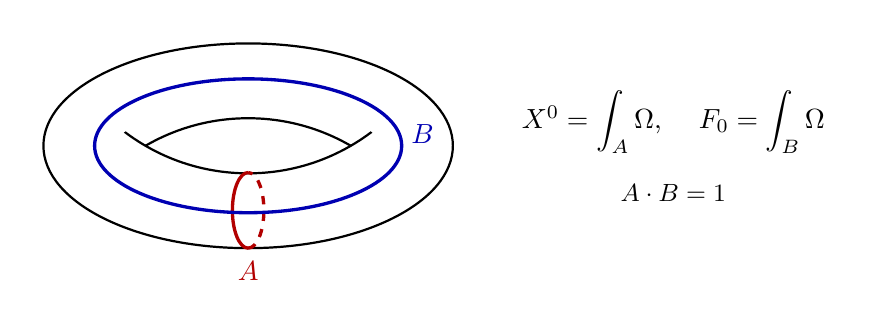
\begin{tikzpicture}[scale=1.0]
    \useasboundingbox (-2.8,-1.9) rectangle (7.6,1.5);
    % トーラス
    \draw[thick] (0,0) ellipse (2.6 and 1.3);
    \begin{scope}
        \clip (0,-1.9) ellipse (2.6 and 2.6);
        \draw[thick] (0,2.25) ellipse (2.6 and 2.6);
    \end{scope}
    \begin{scope}
        \clip (0,2.25) ellipse (2.6 and 2.6);
        \draw[thick] (0,-2.25) ellipse (2.6 and 2.6);
    \end{scope}
    % A サイクル（チューブを一周）
    \draw[very thick, red!70!black] (0,-1.3) arc (270:90:0.2 and 0.48);
    \draw[very thick, red!70!black, dashed] (0,-1.3) arc (-90:90:0.2 and 0.48);
    \node[red!70!black, below] at (0,-1.35) {$A$};
    % B サイクル（穴のまわりを一周）
    \draw[very thick, blue!70!black] (0,0) ellipse (1.95 and 0.85);
    \node[blue!70!black, right] at (1.95,0.15) {$B$};
    % 右：周期
    \node[align=left] at (5.4,0.3) {$X^0 = \displaystyle\int_A \Omega$, \quad $F_0 = \displaystyle\int_B \Omega$};
    \node[align=left, font=\small] at (5.4,-0.6) {$A \cdot B = 1$};
\end{tikzpicture}
\caption{周期の模式図（トーラスの場合）。交叉数 $1$ の2つのサイクル $A$（赤）と $B$（青）の上で正則形式 $\Omega$ を積分したものが周期である。トーラスでは $\Omega = dz$ で、周期の比 $\tau = \int_B\Omega/\int_A\Omega$ が複素構造モジュライとなる。CY3では、$2(h^{2,1} + 1)$ 個の3サイクル $\{A_I, B^I\}$ の上で正則3形式を積分する。}
\label{fig:cycles}
\end{figure}


\paragraph{例：トーラス（1次元のCalabi--Yau多様体）}
2次元トーラス $T^2$ は $c_1 = 0$ の1次元複素多様体であり、Calabi--Yau多様体の最も簡単な例である（図\ref{fig:T2-deformations}）。Hodge数は $h^{1,1} = h^{1,0} = 1$ であり、
\begin{itemize}
    \item \textbf{複素構造モジュライ}：第\ref{ch:intro}章・第\ref{ch:deformation}章の $\tau \in \mathbb{H}$。正則1形式 $\Omega = dz$ の周期の比 $\tau = \int_B dz / \int_A dz$ で与えられる。
    \item \textbf{複素化されたK\"ahlerモジュライ}：$\rho = b + i\,\mathrm{Area}/(4\pi^2\alpha')$（$b$ はB場の積分）。$b \sim b + 1$ の周期性と、$\rho \to -1/\rho$ に対応するT双対性により、$\rho$ も $\mathbb{H}/SL(2, \mathbb{Z})$ に値をとる。
\end{itemize}
\begin{figure}[htbp]
\centering
\begin{tikzpicture}[scale=0.85]
    % 元の格子
    \begin{scope}
        \fill[gray!15] (0,0) -- (2,0) -- (2.6,1.6) -- (0.6,1.6) -- cycle;
        \draw[thick] (0,0) -- (2,0) -- (2.6,1.6) -- (0.6,1.6) -- cycle;
        \node[below] at (1,0) {$1$};
        \node[left] at (0.3,0.85) {$\tau$};
        \node at (1.3,-0.9) {元のトーラス};
    \end{scope}
    % K\"ahler 変形
    \begin{scope}[xshift=4.2cm]
        \fill[blue!15] (0,0) -- (2.8,0) -- (3.64,2.24) -- (0.84,2.24) -- cycle;
        \draw[thick, blue!70!black] (0,0) -- (2.8,0) -- (3.64,2.24) -- (0.84,2.24) -- cycle;
        \draw[gray, dashed] (0,0) -- (2,0) -- (2.6,1.6) -- (0.6,1.6) -- cycle;
        \node at (1.8,-0.9) {K\"ahler変形};
        \node[font=\scriptsize] at (1.8,-1.35) {大きさ（面積）が変わる};
    \end{scope}
    % 複素構造変形
    \begin{scope}[xshift=9.2cm]
        \fill[red!15] (0,0) -- (2,0) -- (3.3,1.3) -- (1.3,1.3) -- cycle;
        \draw[thick, red!70!black] (0,0) -- (2,0) -- (3.3,1.3) -- (1.3,1.3) -- cycle;
        \draw[gray, dashed] (0,0) -- (2,0) -- (2.6,1.6) -- (0.6,1.6) -- cycle;
        \node[left] at (0.75,0.75) {$\tau'$};
        \node at (1.6,-0.9) {複素構造変形};
        \node[font=\scriptsize] at (1.6,-1.35) {形（$\tau$）が変わる};
    \end{scope}
\end{tikzpicture}
\caption{トーラスの2種類の変形。格子の基本平行四辺形（左）を相似に拡大するのがK\"ahler変形（中央）、形の比 $\tau$ を変えるのが複素構造変形（右）である。CY3でも同様に、計量の変形は「大きさ」（$h^{1,1}$ 個）と「形」（$h^{2,1}$ 個）に分かれる。}
\label{fig:T2-deformations}
\end{figure}

弦理論の $T^2$ コンパクト化のモジュライ空間は（局所的に）$\mathcal{M}_\tau \times \mathcal{M}_\rho$ であり、T双対性の一つ（1方向のT双対）は $\tau \leftrightarrow \rho$ を入れ替える。これが次節で述べるミラー対称性の最も簡単な例である。

\section{特殊幾何学（Special Geometry）と有効理論}

4次元の低エネルギー有効理論において、これら $h^{1,1}$ 個のK\"ahlerモジュライと $h^{2,1}$ 個の複素構造モジュライは、質量ゼロのスカラー場として現れる。第\ref{ch:vacuum}章で見たように、これらのスカラー場が張る真空のモジュライ空間 $\mathcal{M}$ は、元の高エネルギー理論から非線形シグマ模型の標的空間として計量を受け継ぐ。

どの超対称性が残り、モジュライがどの多重項に入るかは弦理論の種類によって異なる。
\begin{itemize}
    \item \textbf{タイプII弦理論}：4次元に $\mathcal{N} = 2$ 超対称性が残る。タイプIIAでは $h^{1,1}$ 個のK\"ahlerモジュライがベクトル多重項に、$h^{2,1}$ 個の複素構造モジュライがハイパー多重項に入る（ディラトンはこれとは別の1個の普遍ハイパー多重項に入るので、ハイパー多重項は計 $h^{2,1} + 1$ 個）。タイプIIBでは役割が逆転する。
    \item \textbf{ヘテロティック弦理論}：ゲージ束を入れることで4次元に $\mathcal{N} = 1$ 超対称性が残り、モジュライはカイラル多重項となる。この場合、ゲージ束の変形（束のモジュライ）も加わる。
\end{itemize}

$\mathcal{N} = 2$ 超対称性のもとでは、ベクトル多重項のスカラーのモジュライ空間とハイパー多重項のモジュライ空間は局所的に直積に分解する。
\begin{equation}
    \mathcal{M} = \mathcal{M}_{V} \times \mathcal{M}_{H}
\end{equation}
CY3の幾何学の言葉では、ベクトル多重項のモジュライ空間 $\mathcal{M}_V$ は、タイプIIAではK\"ahlerモジュライ空間 $\mathcal{M}_K$（複素次元 $h^{1,1}$）、タイプIIBでは複素構造モジュライ空間 $\mathcal{M}_C$（複素次元 $h^{2,1}$）そのものである。一方、$\mathcal{M}_H$ は実 $4(h^{2,1} + 1)$ 次元（IIA の場合）の四元数K\"ahler多様体であり、もう一方の幾何学的モジュライはその部分多様体として、RR場の軸子やディラトンとともに含まれる。

\begin{mydef}{特殊K\"ahler多様体（射影的）}{}
複素 $n$ 次元のK\"ahler多様体 $\mathcal{M}$ が\textbf{特殊K\"ahler多様体}であるとは、局所的に射影座標 $X^I$（$I = 0, \dots, n$）と、次数2の斉次正則関数 $\mathcal{F}(X)$（\textbf{プレポテンシャル}）が存在して、K\"ahlerポテンシャルが
\begin{equation*}
    K = -\ln\left[ i\left( \bar{X}^I F_I - X^I \bar{F}_I \right) \right], \qquad F_I = \frac{\partial\mathcal{F}}{\partial X^I}
\end{equation*}
と書けることをいう。
\end{mydef}

$\mathcal{N} = 2$ ベクトル多重項のスカラーのモジュライ空間は、超対称性からこの構造を持つことが示される。（ハイパー多重項のモジュライ空間は四元数K\"ahler多様体という別の構造を持つ。）すなわち、計量・ゲージ結合定数・湯川結合など、有効理論の2微分の相互作用がすべて単一の正則関数 $\mathcal{F}$ から決まる。

\begin{myprop}{CY3の複素構造モジュライの特殊幾何}{special-cx}
CY3の複素構造モジュライ空間 $\mathcal{M}_C$ は特殊K\"ahler多様体であり、射影座標は $A$ 周期 $X^I$、プレポテンシャルの微分は $B$ 周期 $F_I$ で与えられる。K\"ahlerポテンシャル（Weil--Petersson計量のポテンシャル）は
\begin{equation*}
    K = -\ln\left( i\int_X \Omega \wedge \bar{\Omega} \right)
\end{equation*}
である。
\end{myprop}

\begin{note}
$\Omega$ をシンプレクティック基底の双対基底 $\{\alpha_I, \beta^I\}$（$\int_{A_J}\alpha_I = \delta_{IJ}$ など）で展開すると $\Omega = X^I\alpha_I - F_I\beta^I$ であり、Riemann双線形関係 $\int_X \alpha_I \wedge \beta^J = \delta_I^J$ を用いると
\begin{equation*}
    \int_X \Omega \wedge \bar\Omega = -X^I\bar{F}_I + F_I\bar{X}^I
\end{equation*}
となる。よって $i\int_X\Omega\wedge\bar\Omega = i(\bar X^IF_I - X^I\bar F_I)$ であり、特殊K\"ahler多様体の定義の形に一致する（符号はシンプレクティック基底の向きの規約による）。$F_I$ が $X^I$ の関数として $F_I = \partial\mathcal{F}/\partial X^I$ と書けることは、Griffiths横断性 $\int_X \Omega \wedge \partial_I\Omega = 0$ から従う。また、湯川結合は $\kappa_{abc} = \int_X \Omega \wedge \partial_a\partial_b\partial_c\Omega$ で与えられ、$\mathcal{F}$ の3階微分に等しい。
\end{note}

K\"ahlerモジュライ空間 $\mathcal{M}_K$ も古典的には特殊K\"ahler多様体であり、そのプレポテンシャルは $t^a = X^a/X^0$ を用いて
\begin{equation}
    \mathcal{F}_{\text{cl}} = -\frac{1}{6}\frac{\kappa_{abc}X^aX^bX^c}{X^0}, \qquad \kappa_{abc} = \int_X \omega_a \wedge \omega_b \wedge \omega_c
\end{equation}
で与えられる（$\kappa_{abc}$ は2形式の三重交叉数）。このときK\"ahlerポテンシャルは $K = -\ln\left(\frac{4}{3}\int_X J\wedge J\wedge J\right) = -\ln(8\,\mathrm{Vol}(X))$ となり、モジュライ空間の計量はCY3の体積から決まる。ところが、弦理論ではこの古典的なプレポテンシャルに補正が加わる。
\begin{equation}
    \mathcal{F} = \mathcal{F}_{\text{cl}} + (\text{摂動的な } \alpha'^3 \text{ 補正} \propto \zeta(3)\chi(X)) + \sum_{d} n_d\, \mathrm{Li}_3\!\left(e^{2\pi i\, d \cdot t}\right)
\end{equation}
最後の項は、弦が $X$ の中の正則曲線（次数 $d$）に巻き付く\textbf{世界面インスタントン}の寄与であり、$n_d$ は次数 $d$ の有理曲線の「数」（Gromov--Witten不変量に関係する整数）である。

\section{モジュライ空間の特異点：コニフォールド}

複素構造モジュライ空間 $\mathcal{M}_C$ は一般にコンパクトではなく、特異点を持つ。典型的なのは、ある3サイクル（位相的には $S^3$）が潰れる\textbf{コニフォールド点}である。quinticの例では $\psi^5 = 1$ がこれに当たり、そこでは多様体 $X$ 自身が特異点（局所的に $\sum_{i=1}^4 w_i^2 = 0$ という形の錐）を持つ（図\ref{fig:conifold}）。

\begin{figure}[htbp]
\centering
\begin{tikzpicture}
    \foreach \r/\xs/\lab in {0.55/0/{$|z|$ 大}, 0.22/3.6/{$|z|$ 小}, 0.0/7.2/{$z = 0$}} {
        \begin{scope}[xshift=\xs cm]
            \draw[thick] plot[domain=-1.4:1.4, samples=60, smooth] ({-sqrt(\r*\r + 0.5*\x*\x)}, \x);
            \draw[thick] plot[domain=-1.4:1.4, samples=60, smooth] ({sqrt(\r*\r + 0.5*\x*\x)}, \x);
            \draw (0,1.4) ellipse ({sqrt(\r*\r + 0.98)} and 0.15);
            \draw (0,-1.4) ellipse ({sqrt(\r*\r + 0.98)} and 0.15);
            \node at (0,-2.0) {\lab};
        \end{scope}
    }
    % 首の S^3
    \draw[very thick, red!70!black] (0,0) ellipse (0.55 and 0.1);
    \draw[very thick, red!70!black] (3.6,0) ellipse (0.22 and 0.05);
    \fill[red!70!black] (7.2,0) circle (0.06);
    \node[red!70!black, font=\scriptsize] at (0.0,0.35) {$S^3$};
    \node[red!70!black, font=\scriptsize, right] at (7.3,0.05) {特異点};
    \draw[->, thick] (1.4,0) -- (2.3,0);
    \draw[->, thick] (5.0,0) -- (5.9,0);
\end{tikzpicture}
\caption{コニフォールド転移の模式図（3次元の $S^3$ を円で描いている）。複素構造のモジュライ $z = \int_{S^3}\Omega$ を $0$ に近づけると、首の部分の $S^3$（赤）が潰れ、$z = 0$ で多様体は錐状の特異点を持つ。タイプIIB弦理論では、この $S^3$ に巻き付いたD3ブレーンの質量が $|z|$ に比例し、$z \to 0$ で質量ゼロとなる。}
\label{fig:conifold}
\end{figure}


コニフォールド点の近くでは、潰れる $S^3$ 上の周期 $z = \int_{S^3}\Omega$ が局所座標となる。もう一方の双対な周期の振る舞いは、第\ref{ch:intro}章の補足（\ref{sec:modular-supplement}節）と同じ「基底の取り替え」の考え方で理解できる。

\paragraph{モノドロミー＝一周したときの基底の取り替え}
潰れる $S^3$ を $A$、それとちょうど1点で交わる双対な3サイクルを $B$ とし（交点数 $A \cdot B = 1$）、周期を $z = \int_A \Omega$、$F_z = \int_B \Omega$ とする。サイクル $A, B$ は整数係数のホモロジー $H_3(X, \mathbb{Z})$ の基底であり、トーラスの格子の基底 $(\omega_1, \omega_2)$ と同じ役割を果たす。

モジュライ空間の中で $z = 0$ のまわりを1周すると、多様体 $X$ 自身は元に戻る。しかし、サイクルを連続的に追跡していくと、戻ってきたときには一般に\textbf{別の基底}になっている。コニフォールドの場合、その規則は \textbf{Picard--Lefschetzの公式}
\begin{equation*}
    A \mapsto A, \qquad B \mapsto B + (A \cdot B)\, A = B + A
\end{equation*}
で与えられる（潰れるサイクル $A$ 自身は変わらず、それと交わるサイクルが $A$ の分だけずれる）。これは整数係数で交点数を保つ基底の取り替えであり、$(z, F_z)$ に対しては
\begin{equation*}
    \begin{pmatrix} z \\ F_z \end{pmatrix} \mapsto \begin{pmatrix} 1 & 0 \\ 1 & 1 \end{pmatrix} \begin{pmatrix} z \\ F_z \end{pmatrix}, \qquad \begin{pmatrix} 1 & 0 \\ 1 & 1 \end{pmatrix} \in SL(2, \mathbb{Z})
\end{equation*}
と作用する。第\ref{ch:intro}章との違いは、そこでは基底の取り替えが「同じ格子のラベルの付け替え」という冗長性だったのに対し、ここでは特異点のまわりを一周するという操作によって実際に引き起こされる点にある。

1次元低い類比がトーラスである。$q = e^{2\pi i\tau} \to 0$（カスプ $\mathrm{Im}\,\tau \to \infty$）ではトーラスの1つのサイクルが相対的に潰れ、$q = 0$ のまわりを1周すると $\tau \mapsto \tau + 1$、すなわち $T$ が生じる。これはまさに図\ref{fig:T-cut-paste}の Dehn ツイスト（$b \mapsto b + a$）であり、Picard--Lefschetzの公式の最も簡単な例になっている。

\paragraph{モノドロミーから対数が決まる}
$z \mapsto e^{2\pi i}z$ で $F_z \mapsto F_z + z$ となることが分かれば、$F_z$ の形はほぼ決まる。$\ln z \mapsto \ln z + 2\pi i$ であるから、$F_z - \frac{z}{2\pi i}\ln z$ は $z = 0$ のまわりで一価であり、$z \to 0$ で有界なので（除去可能特異点として）正則である。よって
\begin{equation}
    F_z \simeq \frac{z}{2\pi i}\ln z + (\text{正則})
\end{equation}
という対数的な振る舞いが従う。すなわち、$z$ の周りを1周すると $F_z \to F_z + z$ という\textbf{モノドロミー}が生じ、モジュライ空間の計量 $g_{z\bar z} \sim -\ln|z|^2$ は $z \to 0$ で対数的に発散する（ただし原点までの距離は有限）。

\begin{note}
一見すると、これは低エネルギー有効理論が $z = 0$ で破綻していることを示しているように見える。Stromingerはこの問題を次のように解決した\cite{strominger1995}。タイプIIB弦理論では、D3ブレーンが潰れる $S^3$ に巻き付いた状態は、質量が周期に比例する $M \propto |z|$ 粒子（4次元ではブラックホール）として振る舞う。$z \to 0$ でこの粒子は\textbf{質量ゼロ}となり、有効理論から積分消去してはならない新たな軽い自由度となる。対数的な特異性は、まさにこの質量ゼロの荷電粒子を積分消去したことによる1ループの効果（Seiberg--Witten理論のモノポールと同じ機構）として再現される。

ここでも、第\ref{ch:instanton}章（小インスタントン）や第\ref{ch:vacuum}章（Seiberg--Witten）と全く同じく、\textbf{モジュライ空間の特異点 $=$ 新しい軽い自由度の出現点}という原理が働いている。
\end{note}

\section{ミラー対称性の予兆}

最後に、モジュライ空間の分解が示唆する深遠な双対性について触れておく。弦理論の枠組みでは、あるCY3 $X$ 上でコンパクト化された理論と、全く別のCY3 $Y$ 上でコンパクト化された理論が、物理的に全く同等になることがある。より正確には、$X$ 上のタイプIIA弦理論と $Y$ 上のタイプIIB弦理論が同等であり、このとき $X$ のK\"ahlerモジュライ空間と $Y$ の複素構造モジュライ空間が入れ替わっている。
\begin{equation}
    h^{1,1}(X) = h^{2,1}(Y), \quad h^{2,1}(X) = h^{1,1}(Y), \qquad \mathcal{M}_K(X) \cong \mathcal{M}_C(Y)
\end{equation}
これを\textbf{ミラー対称性（Mirror Symmetry）}と呼ぶ（図\ref{fig:mirror}）。Euler数は $\chi(X) = -\chi(Y)$ と符号が反転する。quintic（$h^{1,1} = 1,\ h^{2,1} = 101$）のミラー $Y$ は $h^{1,1} = 101,\ h^{2,1} = 1$ を持ち、その1次元の複素構造モジュライ空間がquinticのK\"ahlerモジュライ空間に対応する。

\begin{figure}[htbp]
\centering
\begin{tikzpicture}[box/.style={draw, thick, rounded corners, minimum width=3.2cm, minimum height=0.8cm, align=center}]
    \node[box, fill=blue!8] (A) at (0,2) {タイプIIA 弦理論 on $X$};
    \node[box, fill=red!8] (B) at (7,2) {タイプIIB 弦理論 on $Y$};
    \draw[<->, very thick] (A) -- node[above] {物理的に同等} (B);
    \node[box] (KX) at (0,0.5) {$\mathcal{M}_K(X)$\\{\scriptsize $h^{1,1}(X)$ 次元・量子補正あり}};
    \node[box] (CX) at (0,-1.2) {$\mathcal{M}_C(X)$\\{\scriptsize $h^{2,1}(X)$ 次元}};
    \node[box] (KY) at (7,-1.2) {$\mathcal{M}_K(Y)$\\{\scriptsize $h^{1,1}(Y)$ 次元}};
    \node[box] (CY) at (7,0.5) {$\mathcal{M}_C(Y)$\\{\scriptsize $h^{2,1}(Y)$ 次元・古典的に厳密}};
    \draw[<->, very thick, blue!70!black] (KX) -- node[above, font=\scriptsize] {ミラー写像} (CY);
    \draw[<->, very thick, red!70!black] (CX) -- (KY);
\end{tikzpicture}
\caption{ミラー対称性。$X$ 上のタイプIIA弦理論と $Y$ 上のタイプIIB弦理論が同等であり、$X$ のK\"ahlerモジュライ空間と $Y$ の複素構造モジュライ空間（およびその逆）が入れ替わる。世界面インスタントンの補正を含む左上の量を、古典的な周期積分で厳密に計算できる右上の量に翻訳できる。}
\label{fig:mirror}
\end{figure}

K\"ahlerモジュライ空間の計量には、前節で見た世界面インスタントンに由来する無限個の補正が含まれており、これを直接計算することは極めて困難である。しかし、複素構造モジュライ空間の計量は古典的な周期積分だけで厳密に定まり、量子補正を受けない（タイプIIBではディラトンがハイパー多重項に入るため、ベクトル多重項のモジュライ空間は $g_s$ 補正も受けず、また世界面の計算でも $\alpha'$ に依存しない）。ミラー対称性を用いれば、計算が困難なK\"ahler幾何学（量子幾何学）の情報を、双対な多様体の複素幾何学（古典幾何学）の周期積分に翻訳して解くことができる。

\paragraph{例：quinticの有理曲線の数え上げ}
Candelas, de la Ossa, Green, Parkesは1991年\cite{candelas1991}、ミラー多様体の周期積分（Picard--Fuchs方程式の解）を計算し、それをミラー写像でquinticのK\"ahlerモジュライに翻訳することで、quintic上の次数 $d$ の有理曲線の数 $n_d$ を予言した。
\begin{equation}
    n_1 = 2875, \qquad n_2 = 609250, \qquad n_3 = 317206375, \quad \dots
\end{equation}
$n_1 = 2875$（直線の数）と $n_2 = 609250$（2次曲線の数）は古典的な代数幾何学で知られていたが、$n_3$ 以降は物理からの予言であり、後に数学的に証明された。モジュライ空間の代数幾何学的な構造が、弦理論の非摂動的なダイナミクスを厳密に解き明かす最強の武器となるのである。

\begin{note}
現象論的な観点からは、質量ゼロのモジュライ場は観測と矛盾する（長距離の第5の力や、宇宙論的なモジュライ問題を引き起こす）。したがって現実的なコンパクト化では、モジュライに質量を与えて真空のモジュライ空間の特定の点に固定する\textbf{モジュライ安定化}が必要となる。タイプIIBでは、3形式フラックスを入れることで超ポテンシャル $W = \int_X G_3 \wedge \Omega$（Gukov--Vafa--Witten\cite{gvw2000}）が生じ、複素構造モジュライとディラトンが固定される。K\"ahlerモジュライは非摂動効果（D7ブレーン上のゲージーノ凝縮など）で固定される（KKLT\cite{kklt2003}）。これは第\ref{ch:vacuum}章で見た「量子効果によるモジュライ空間の持ち上がり」の弦理論版である。
\end{note}
\chapter{一般相対論・幾何構造：計量や曲面の分類}
\label{ch:gravity}

これまでの章では、固定された背景時空（ミンコフスキー時空など）の上で定義されるゲージ場やスカラー場のモジュライ空間を考察してきた。しかし、一般相対性理論においては「時空の計量（Metric）」そのものが力学変数として振る舞う。本章では、計量のなす無限次元空間を微分同相写像で割った商空間（モジュライ空間）の構造を調べ、重力場における真の物理的自由度がどのように抽出されるのかを議論する。

特に、2次元の計量のモジュライ空間は、本章の後半で扱う「リーマン面のモジュライ（Teichm\"uller空間）」に一致し、局所的な自由度がゼロになるという劇的な帰結をもたらす。第\ref{ch:group-action}章の商空間、第\ref{ch:deformation}章の変形理論と指数定理、第\ref{ch:bundle}章のGauss--Bonnetの定理が、ここで重力の言葉に翻訳される。

\section{計量の空間と微分同相群による商}

多様体 $M$ 上の滑らかな計量テンソル $g_{\mu\nu}(x)$ の全体がなす空間を $\mathrm{Met}(M)$ と表す。計量テンソルは対称テンソルであるため、$D$ 次元多様体においては各点で $\frac{1}{2}D(D+1)$ 個の独立な成分を持つ。

一般相対論における「ゲージ対称性」とは、任意の座標変換の自由度、すなわち多様体 $M$ 上の微分同相写像のなす群 $\mathrm{Diff}(M)$ である。微分同相写像 $f: M \to M$ のもとで、計量は引き戻し（pull-back）$f^* g$ によって変換される。真の物理的な時空の幾何学は、特定の座標系の取り方に依存しない。

\begin{mydef}{幾何のモジュライ空間}{}
$\mathrm{Diff}(M)$ は $\mathrm{Met}(M)$ に引き戻し $g \mapsto f^*g$ で（右から）作用する。その商空間
\begin{equation*}
    \mathcal{M}_{\text{geom}}(M) = \mathrm{Met}(M) / \mathrm{Diff}(M)
\end{equation*}
を、$M$ 上の\textbf{幾何（計量の同値類）のモジュライ空間}と呼ぶ。運動方程式（例えばEinstein方程式）を満たす計量に制限したものを、その方程式の解のモジュライ空間と呼ぶ。
\end{mydef}

この作用は一般には自由ではない。計量 $g$ における固定部分群は、$g$ の\textbf{等長変換群} $\mathrm{Isom}(M, g)$ であり、そのリー代数はKillingベクトル場 $\nabla_\mu\xi_\nu + \nabla_\nu\xi_\mu = 0$ の空間である。第\ref{ch:group-action}章の一般論がそのまま当てはまる。$M$ がコンパクトならば $\mathrm{Isom}(M, g)$ はコンパクトなリー群であり、Ebinのスライス定理\cite{ebin1970}により、$\mathrm{Met}(M)/\mathrm{Diff}(M)$ は等長変換群を持たない計量の近傍では（無限次元の）多様体、有限の等長変換群を持つ計量の近傍ではオービフォールド、連続的な等長変換群を持つ計量の近傍ではより深刻な特異点を持つ。対称性の高い計量ほど、モジュライ空間の特異な点に位置するのである。

\paragraph{例：平坦トーラスのモジュライ}
$n$ 次元トーラス $T^n = \mathbb{R}^n/\mathbb{Z}^n$ 上の平坦な計量は、定数行列 $g_{ij}$（正定値対称）で与えられる。座標の線形変換で $\mathbb{Z}^n$ を保つもの、すなわち $GL(n, \mathbb{Z})$ による変換で移り合う計量は同じ幾何を与えるので、平坦計量のモジュライ空間は
\begin{equation}
    \mathcal{M}_{\text{flat}}(T^n) = \left\{ \text{正定値対称行列 } g_{ij} \right\} / GL(n, \mathbb{Z}) \cong GL(n, \mathbb{Z}) \backslash GL(n, \mathbb{R}) / O(n)
\end{equation}
となり、その次元は $\frac{1}{2}n(n+1)$ である。$n = 2$ では、全体の面積（1次元）と形 $\tau \in \mathbb{H}/SL(2, \mathbb{Z})$（2次元）に分かれ、第\ref{ch:intro}章のトーラスのモジュライ空間が再現される。$T^n$ はCalabi--Yau多様体の最も簡単な例でもあり、第\ref{ch:calabi-yau}章のRicci平坦計量のモジュライの原型である。

\paragraph{Wheelerのスーパースペース}
正準量子重力では、時空 $M = \mathbb{R} \times \Sigma$ を時間方向と空間 $\Sigma$（3次元）に分解し、空間の計量 $h_{ij}$ を正準変数とする。このとき物理的な配位空間は、\textbf{空間の}計量の空間を空間の微分同相で割った
\begin{equation}
    \mathcal{S}(\Sigma) = \mathrm{Riem}(\Sigma) / \mathrm{Diff}(\Sigma)
\end{equation}
であり、Wheelerはこれを\textbf{スーパースペース（Superspace）}と呼んだ（超対称性のスーパースペースとは異なる概念であることに注意）。時間方向の微分同相（時間の取り直し）に対応する拘束条件はハミルトニアン拘束として残り、量子論ではスーパースペース上の波動関数に対する\textbf{Wheeler--DeWitt方程式} $\hat{\mathcal{H}}\Psi[h] = 0$ となる。

\section{作用の変形と物理的自由度の数え上げ}

真空の一般相対論のダイナミクスは、Einstein--Hilbert作用によって記述される。
\begin{equation}
    S_{EH} = \frac{1}{16\pi G_N} \int_M d^D x \sqrt{-g}\, R
\end{equation}
ここで $g = \det(g_{\mu\nu})$ であり、$R$ はスカラー曲率である。モジュライ空間の接ベクトル（運動方程式を満たす物理的な無限小変形）を抽出するために、計量を $g_{\mu\nu} \to g_{\mu\nu} + \delta g_{\mu\nu}$ と変形し、作用の停留条件を計算する。

\begin{note}
計量の変分に対する曲率の変分を計算しよう。まず、逆計量と行列式の変分は以下のようになる。
\begin{equation*}
    \delta g^{\mu\nu} = - g^{\mu\rho} g^{\nu\sigma} \delta g_{\rho\sigma}, \quad \delta \sqrt{-g} = \frac{1}{2} \sqrt{-g}\, g^{\mu\nu} \delta g_{\mu\nu}
\end{equation*}
次に、Levi-Civita接続（Christoffel記号 $\Gamma^\rho_{\mu\nu}$）の変分 $\delta \Gamma^\rho_{\mu\nu}$ を考える。$\Gamma$ 自身はテンソルではないが、2つの接続の差はテンソルである（第\ref{ch:bundle}章で見た「接続の空間はアフィン空間」の重力版）ので、その変分は共変微分 $\nabla$ を用いて次のように書ける。
\begin{equation*}
    \delta \Gamma^\rho_{\mu\nu} = \frac{1}{2} g^{\rho\sigma} \left( \nabla_\mu \delta g_{\nu\sigma} + \nabla_\nu \delta g_{\mu\sigma} - \nabla_\sigma \delta g_{\mu\nu} \right)
\end{equation*}
Ricciテンソル $R_{\mu\nu} = \partial_\rho \Gamma^\rho_{\mu\nu} - \dots$ の変分は、Palatiniの恒等式として知られる以下の式になる。
\begin{equation*}
    \delta R_{\mu\nu} = \nabla_\rho (\delta \Gamma^\rho_{\mu\nu}) - \nabla_\nu (\delta \Gamma^\rho_{\mu\rho})
\end{equation*}
作用の変分を計算すると、
\begin{align*}
    \delta (\sqrt{-g} R) &= \delta (\sqrt{-g}\, g^{\mu\nu} R_{\mu\nu}) \\
    &= (\delta \sqrt{-g}) R + \sqrt{-g}\, (\delta g^{\mu\nu}) R_{\mu\nu} + \sqrt{-g}\, g^{\mu\nu} \delta R_{\mu\nu} \\
    &= \sqrt{-g} \left[ \frac{1}{2} g^{\mu\nu} R - R^{\mu\nu} \right] \delta g_{\mu\nu} + \sqrt{-g}\, \nabla_\rho V^\rho
\end{align*}
となる（$V^\rho = g^{\mu\nu}\delta\Gamma^\rho_{\mu\nu} - g^{\mu\rho}\delta\Gamma^\nu_{\mu\nu}$）。表面項 $\nabla_\rho V^\rho$ を無視すると、作用が任意の変形 $\delta g_{\mu\nu}$ に対して停留する条件として、Einstein方程式 $R_{\mu\nu} - \frac{1}{2} g_{\mu\nu} R = 0$ が得られる。
\end{note}

さて、線形化された重力波（微小な計量の揺らぎ）の「物理的な自由度」の数を数えてみよう。計量 $g_{\mu\nu}$ は $\frac{1}{2}D(D+1)$ 個の成分を持つ。一方、無限小の微分同相変換は、ベクトル場 $\xi^\mu(x)$ に沿ったLie微分 $\mathcal{L}_\xi$ で与えられ、計量テンソルの変分は
\begin{equation}
    \delta_\xi g_{\mu\nu} = \nabla_\mu \xi_\nu + \nabla_\nu \xi_\mu
\end{equation}
となる。ベクトル場 $\xi^\mu$ は $D$ 個の任意関数を含む。

\begin{myprop}{重力子の自由度}{graviton-dof}
$D$ 次元の一般相対論において、伝播する（局所的な）物理的自由度の数は
\begin{equation*}
    \frac{1}{2}D(D+1) - 2D = \frac{1}{2}D(D-3)
\end{equation*}
である。
\end{myprop}

ゲージ自由度は「2回」差し引かれることに注意しよう。1回目はゲージ固定（$D$ 個のゲージ条件、例えば調和ゲージ $\nabla^\mu \bar{h}_{\mu\nu} = 0$）であり、2回目は、ゲージ固定後もなお残る残余ゲージ変換、あるいは同じことだが時間発展を含まない $D$ 個の拘束条件（Einstein方程式の $G_{0\mu}$ 成分）である。これは電磁気学において $A_\mu$ の $D$ 成分からゲージ固定と Gauss則で2つが除かれ、$D - 2$ 個の偏極が残るのと同じ構造である。

\begin{itemize}
    \item $D = 4$：$\frac{1}{2} \times 4 \times 1 = 2$。重力波が2つの偏極モード（プラス・モードとクロス・モード）を持つという事実と一致する。
    \item $D = 3$：$\frac{1}{2} \times 3 \times 0 = 0$。3次元重力には伝播する重力子が存在しない。それでも理論は自明ではなく、大域的な自由度が残る。実際、3次元の重力は（宇宙項に応じて）$ISO(2,1)$ や $SO(2,2)$ などをゲージ群とするChern--Simons理論として書き直され、その解のモジュライ空間は第\ref{ch:deformation}章で扱った\textbf{平坦接続のモジュライ空間} $\mathrm{Hom}(\pi_1(\Sigma), G)/G$ に一致する\cite{witten1988}。
    \item $D = 2$：$\frac{1}{2} \times 2 \times (-1) = -1$。自由度が負になってしまう。これは次節で解消される。
\end{itemize}

\section{2次元重力とWeyl不変性：局所自由度の消失}

上記の公式で $D = 2$ とすると物理的な自由度が負になってしまうように見える。このパラドックスは、弦理論の世界面上の量子重力を理解する上で最も重要な出発点となる。

まず、2次元ではEinstein--Hilbert作用そのものが力学を持たない。

\begin{myprop}{2次元のEinstein--Hilbert作用}{2d-EH}
閉曲面 $\Sigma$ 上のEuclid化されたEinstein--Hilbert作用はトポロジカルであり、
\begin{equation*}
    \frac{1}{4\pi}\int_\Sigma d^2x \sqrt{g}\, R = \chi(\Sigma) = 2 - 2g
\end{equation*}
が任意の計量に対して成り立つ。特に、その変分は恒等的にゼロである（$R_{ab} - \frac{1}{2}g_{ab}R \equiv 0$）。
\end{myprop}

\begin{note}
2次元ではスカラー曲率はGauss曲率の2倍 $R = 2K$ であり、面積要素は $dA = \sqrt{g}\,d^2x$ である。したがって左辺は $\frac{1}{2\pi}\int_\Sigma K\, dA$ であり、第\ref{ch:bundle}章で特性類の例として見たGauss--Bonnetの定理により $\chi(\Sigma)$ に等しい。また2次元では、Riemann曲率テンソルの独立成分は1つだけで $R_{abcd} = \frac{R}{2}(g_{ac}g_{bd} - g_{ad}g_{bc})$ と書けるので、縮約して $R_{ab} = \frac{R}{2}g_{ab}$、すなわちEinsteinテンソルは恒等的にゼロである。
\end{note}

したがって、2次元の重力の作用は位相不変量 $\chi$ に比例する項だけであり、弦理論ではこれが弦の結合定数 $g_s^{-\chi}$ の重みとして種数展開を与える。弦の力学は、世界面の計量 $g_{ab}$ に結合した物質場（埋め込み $X^\mu$）の\textbf{Polyakov作用}
\begin{equation}
    S_P = \frac{1}{4\pi\alpha'}\int_\Sigma d^2\sigma \sqrt{g}\, g^{ab}\partial_a X^\mu \partial_b X_\mu
\end{equation}
で記述される\cite{polchinskistringtheoryvolume12005}。この作用は微分同相に加えて、計量の局所的なスケール変換（\textbf{Weyl変換}）
\begin{equation}
    g_{ab}(x) \to e^{2\omega(x)} g_{ab}(x)
\end{equation}
に対しても不変である（2次元では $\sqrt{g}\,g^{ab}$ がWeyl不変であるため）。

2次元多様体上の計量は $\frac{1}{2} \times 2 \times 3 = 3$ 個の独立な成分を持つ。これに対して、微分同相変換 $\xi^a$ は2つ、Weyl変換のパラメータ $\omega(x)$ は1つの局所自由度を持ち、対称性の自由度は計 $2 + 1 = 3$ となる。

\begin{note}
微小変形における自由度を式で確認する。微小な微分同相変換 $\xi^a$ と微小なWeyl変換 $\omega$ による計量の変化は、
\begin{equation*}
    \delta g_{ab} = \nabla_a \xi_b + \nabla_b \xi_a + 2\omega\, g_{ab}
\end{equation*}
である。これをトレースレス部分とトレース部分に分けると
\begin{equation*}
    \delta g_{ab} = (P_1\xi)_{ab} + (2\omega + \nabla\cdot\xi)\, g_{ab}, \qquad (P_1\xi)_{ab} \equiv \nabla_a\xi_b + \nabla_b\xi_a - g_{ab}\nabla\cdot\xi
\end{equation*}
となる。トレース部分（1成分）は $\omega$ で任意に動かせ、トレースレス部分（2成分）は $\xi^a$（2成分）に作用する1階の微分作用素 $P_1$ で動かせる。したがって局所的には、任意の計量変形はゲージ変換で打ち消せる。
\end{note}

局所的な自由度の収支は $3 - (2 + 1) = 0$ となる。すなわち、\textbf{2次元重力においては局所的に伝播する重力子（グラビトン）は存在しない}。これを有限の変換の言葉で述べたのが、次の定理である。

\begin{mythm}{等温座標の存在}{isothermal}
2次元Riemann多様体の任意の点の近傍には、計量が $g = e^{2\omega(x)}(dx^2 + dy^2)$ という形になる座標（\textbf{等温座標}）が存在する。すなわち、任意の2次元計量は局所的に共形平坦である。
\end{mythm}

等温座標 $z = x + iy$ どうしの座標変換は（向きを保つならば）正則関数で与えられるので、2次元の向き付けられたRiemann多様体には自然に\textbf{複素構造}が定まり、リーマン面となる。すなわち、「計量をWeyl変換で割ったもの（共形構造）」と「複素構造」は同じものである。

\section{大域的なモジュライとTeichm\"uller空間への帰着}

局所的な自由度がゼロであるからといって、計量のモジュライ空間が「1つの点」に潰れてしまうわけではない。第\ref{ch:intro}章のトーラスの例で先取りしたように、曲面 $\Sigma$ のトポロジー（種数 $g$）が非自明な場合、滑らかな座標変換とWeyl変換を尽くしても決して相殺できない\textbf{「大域的な」計量の自由度}が残るのである。まず、各共形類の中から標準的な代表元を選べることが重要である。

\begin{mythm}{一意化定理}{uniformization}
種数 $g$ の閉曲面 $\Sigma$ 上の任意の計量は、Weyl変換によって定曲率計量に移すことができる。その定曲率計量は、$g \ge 2$ ではただ一つ、$g = 1$ では面積を固定すればただ一つである。$g = 0$ では共形変換群 $PSL(2, \mathbb{C})$ の分だけ自由度が残り、一意性は微分同相を除いてのみ成り立つ（これは後述の、球面が6個の共形Killingベクトルを持つことに対応する）。曲率の符号は種数で決まり、
\begin{equation*}
    K = +1\ (g = 0), \qquad K = 0,\ \text{面積} = 1\ (g = 1), \qquad K = -1\ (g \ge 2)
\end{equation*}
である。
\end{mythm}

曲率の符号は、Gauss--Bonnetの定理 $\int K\, dA = 2\pi(2 - 2g)$ と整合している。したがって、Weyl変換で割ることは「定曲率計量に制限すること」と同じであり、残る問題は定曲率計量を微分同相で分類することになる。

\begin{mydef}{Teichm\"uller空間と写像類群}{}
微分同相変換群 $\mathrm{Diff}(\Sigma)$ の単位元と連続的につながっている部分群を $\mathrm{Diff}_0(\Sigma)$、Weyl変換の群を $\mathrm{Weyl}(\Sigma)$ とする。
\begin{enumerate}
    \item 商空間
    \begin{equation*}
        \mathcal{T}_g = \frac{\mathrm{Met}(\Sigma)}{\mathrm{Diff}_0(\Sigma) \ltimes \mathrm{Weyl}(\Sigma)}
    \end{equation*}
    を\textbf{Teichm\"uller空間}と呼ぶ。
    \item 連続変形できない「大きな座標変換」のなす群
    \begin{equation*}
        \Gamma_g = \mathrm{Diff}^+(\Sigma) / \mathrm{Diff}_0(\Sigma)
    \end{equation*}
    を\textbf{写像類群（Mapping Class Group）}と呼ぶ（$\mathrm{Diff}^+$ は向きを保つ微分同相）。
    \item リーマン面のモジュライ空間を $\mathcal{M}_g = \mathcal{T}_g / \Gamma_g$ で定める。
\end{enumerate}
\end{mydef}

\begin{myprop}{Teichm\"uller空間の構造}{teichmuller}
\begin{enumerate}
    \item $g \ge 2$ のとき、$\mathcal{T}_g$ は $\mathbb{R}^{6g-6}$ と同相（特に可縮）であり、複素次元 $3g - 3$ の複素多様体である。
    \item 写像類群 $\Gamma_g$ は $\mathcal{T}_g$ に真性不連続に作用するので、$\mathcal{M}_g = \mathcal{T}_g / \Gamma_g$ はオービフォールドである（第\ref{ch:group-action}章）。
    \item $g = 1$ のとき、$\mathcal{T}_1 = \mathbb{H}$、$\Gamma_1 = SL(2, \mathbb{Z})$ であり、$\mathcal{M}_1 = \mathbb{H}/SL(2, \mathbb{Z})$ は第\ref{ch:intro}章のトーラスのモジュライ空間に一致する。
\end{enumerate}
\end{myprop}

$\mathcal{T}_g$ の次元は、第\ref{ch:deformation}章で計算した $\dim_{\mathbb{C}} H^1(\Sigma, T_\Sigma) = 3g - 3$ に一致している。これは偶然ではなく、計量の変形の言葉で直接見ることができる。

\begin{note}
前節の作用素 $P_1$（ベクトル場 $\to$ トレースレス対称テンソル）を考える。トレースレスな計量変形 $\delta g$ のうち、$\mathrm{im}\, P_1$（微分同相）で動かせないものがモジュライの方向であり、$L^2$ 内積で直交補空間をとると、それは $\ker P_1^\dagger$（\textbf{正則2次微分}、第\ref{ch:deformation}章の $H^0(\Sigma, K^2)$）と同一視される。一方 $\ker P_1$ は計量を保つ（Weyl変換を除いて）ベクトル場、すなわち\textbf{共形Killingベクトル}であり、第\ref{ch:deformation}章の $H^0(\Sigma, T_\Sigma)$ に対応する。Riemann--Rochの定理（あるいは $P_1$ に対する指数定理）を実次元で書くと
\begin{equation*}
    \dim_{\mathbb{R}} \ker P_1^\dagger - \dim_{\mathbb{R}} \ker P_1 = 6g - 6
\end{equation*}
である。
\begin{itemize}
    \item $g \ge 2$：共形Killingベクトルはなく（$\ker P_1 = 0$）、モジュライは $6g - 6$ 個。
    \item $g = 1$：共形Killingベクトルは並進の2個、モジュライは $\tau$ の2個（実次元）。
    \item $g = 0$：共形Killingベクトルは $PSL(2, \mathbb{C})$ の6個、モジュライは0個。
\end{itemize}
これは第\ref{ch:deformation}章の命題（リーマン面の変形と自己同型）を、計量の言葉で言い直したものである。
\end{note}

弦理論における散乱振幅の計算は、すべての計量についての無限次元の経路積分が、Faddeev--Popovゴーストの行列式（測度）を伴って、この有限次元空間 $\mathcal{M}_g$ 上の積分へと劇的に還元されることを意味する\cite{polchinskistringtheoryvolume12005}。モジュライ方向の $6g-6$ 個の積分にはそれぞれ $b$ ゴーストの零モードが対応し（第\ref{ch:deformation}章）、共形Killingベクトル（$c$ ゴーストの零モード）は頂点演算子の位置を固定することで処理される。重力のダイナミクスが、完全に代数幾何学的な「モジュライ積分」に帰着するのである。

このリーマン面のモジュライ空間の構造、とくに境界の退化（コンパクト化）やモジュライ・スタックとしての性質は、本講義の範囲を超えるため、第III部（予定）で扱う。

\appendix

\chapter{代数トポロジーの基礎}
\label{app:topology}

本文では、基本群・ホモトピー群・写像度・de Rhamコホモロジー・ホモロジーといった代数トポロジーの概念を、モジュライ空間やゲージ場の大域的な性質を調べる道具として繰り返し用いた。この付録では、それらを本文で必要になる範囲で、定義・直観・代表的な例・本文での使われ方の順にまとめる。証明は概略にとどめ、厳密な扱いは標準的な教科書（例えば Hatcher『Algebraic Topology』、Bott--Tu『Differential Forms in Algebraic Topology』、中原『理論物理学のための幾何学とトポロジー』）に譲る。

全体を貫く考え方は次の1つである。
\begin{quote}
\textbf{連続的に変形しても変わらない量（位相不変量）は、整数や群のような離散的な値をとり、空間の「穴」や「ねじれ」を検出する。}
\end{quote}
物理では、これがトポロジカルな電荷（磁荷・インスタントン数・巻き付き数）の量子化や、大域的なゲージ固定の不可能性として現れる。

%==============================================================
\section{ホモトピーと可縮性}
\label{sec:topo-homotopy}

\begin{mydef}{ホモトピー}{}
2つの連続写像 $f_0, f_1: X \to Y$ が\textbf{ホモトピック}であるとは、連続写像 $F: X \times [0, 1] \to Y$ で $F(x, 0) = f_0(x)$、$F(x, 1) = f_1(x)$ を満たすものが存在することをいう。$F$ を\textbf{ホモトピー}と呼び、$f_0 \simeq f_1$ と書く。
\end{mydef}

$F(\cdot, t)$ は「時刻 $t$ における写像」であり、ホモトピーとは写像の連続的な変形のことである。ホモトピックという関係は同値関係であり、その同値類を\textbf{ホモトピー類}と呼ぶ。物理の言葉では、場の配位 $f: X \to Y$（例えば時空から標的空間への写像）の空間の\textbf{連結成分}がホモトピー類である。有限のエネルギー障壁を越えずに移り合える配位は同じホモトピー類に属し、異なるホモトピー類の間を移るには場がどこかで特異にならなければならない。

\begin{mydef}{ホモトピー同値・可縮}{}
連続写像 $f: X \to Y$、$g: Y \to X$ で $g \circ f \simeq \mathrm{id}_X$、$f \circ g \simeq \mathrm{id}_Y$ となるものが存在するとき、$X$ と $Y$ は\textbf{ホモトピー同値}であるという。1点とホモトピー同値な空間、すなわち恒等写像が定値写像にホモトピックな空間を\textbf{可縮}という。
\end{mydef}

\paragraph{例}
\begin{itemize}
    \item $\mathbb{R}^n$ は $F(x, t) = (1 - t)x$ によって原点に縮められるので可縮である。より一般に、ある点 $x_0$ から各点への線分を含む領域（星形領域）は可縮である。
    \item ゲージ接続の空間 $\mathcal{A}$ はアフィン空間なので、同じ理由で可縮である（第\ref{ch:bundle}章）。
    \item $\mathbb{R}^n \setminus \{0\}$ は球面 $S^{n-1}$ とホモトピー同値である（$x \mapsto x/|x|$ で単位球面に縮められる）。第\ref{ch:group-action}章で $\mathbb{C}^{n+1} \setminus \{0\}$ を $S^{2n+1}$ に縮めたのはこの例である。
    \item 球面 $S^n$ は可縮ではない（\ref{sec:topo-degree}節で写像度を用いて示す）。
\end{itemize}

以下で導入する基本群・ホモトピー群・de Rhamコホモロジー・ホモロジーはすべて\textbf{ホモトピー不変}、すなわちホモトピー同値な空間に対して同型な群を与える。特に同相な空間に対しては同型である。したがって、これらの群が異なれば2つの空間は同相ではない、と結論できる。

%==============================================================
\section{被覆空間}
\label{sec:topo-covering}

\begin{mydef}{被覆}{}
連続な全射 $p: \tilde{X} \to X$ が\textbf{被覆写像}であるとは、$X$ の各点が開近傍 $U$ を持ち、$p^{-1}(U)$ が互いに交わらない開集合 $\tilde{U}_\alpha$ の和で、各 $p|_{\tilde{U}_\alpha}: \tilde{U}_\alpha \to U$ が同相であることをいう。各 $\tilde{U}_\alpha$ を\textbf{シート}と呼び、シートの数が $m$ のとき $m$ 重被覆という。
\end{mydef}

局所的には $\tilde{X}$ は $X$ のコピーを何枚も重ねたものに見えるが、大域的にはシートどうしがつながっている。離散群 $\Gamma$ が多様体 $\tilde{X}$ に自由かつ固有に作用するとき、商写像 $\tilde{X} \to \tilde{X}/\Gamma$ は被覆写像である（第\ref{ch:group-action}章の商多様体定理で $G$ が離散群の場合。ファイバーが離散的な主束と言ってもよい）。

\paragraph{例}
\begin{center}
\begin{tabular}{lll}
    \hline
    被覆 & 群 $\Gamma$ & 本文での登場 \\
    \hline
    $\mathbb{R} \to S^1 = \mathbb{R}/\mathbb{Z}$ & $\mathbb{Z}$ & 周期的境界条件（第\ref{ch:group-action}章） \\
    $\mathbb{C} \to E_\Lambda = \mathbb{C}/\Lambda$ & $\Lambda \cong \mathbb{Z}^2$ & トーラス（第\ref{ch:intro}章） \\
    $S^1 \to S^1$、$z \mapsto z^m$ & $\mathbb{Z}_m$ & 写像度 $m$ の写像（\ref{sec:topo-degree}節） \\
    $S^n \to \mathbb{RP}^n$ & $\mathbb{Z}_2 = \{\pm 1\}$ & 実Hopf束（第\ref{ch:instanton}章） \\
    $SU(2) \to SO(3)$ & $\mathbb{Z}_2$ & スピノル（第\ref{ch:instanton}章） \\
    \hline
\end{tabular}
\end{center}

\paragraph{持ち上げ}
被覆の最も重要な性質は\textbf{道の持ち上げ}である。$X$ 上の道 $\gamma: [0, 1] \to X$ と、始点の上の点 $\tilde{x}_0 \in p^{-1}(\gamma(0))$ を与えると、$p \circ \tilde{\gamma} = \gamma$、$\tilde{\gamma}(0) = \tilde{x}_0$ を満たす道 $\tilde{\gamma}$ が\textbf{ただ1つ}存在する（各シートの上では $p$ が同相なので、短い区間ごとに一意に持ち上げられる）。同様にホモトピーも持ち上げられる。例えば $\mathbb{R} \to S^1$、$t \mapsto e^{2\pi i t}$ では、$S^1$ 上のループを $\mathbb{R}$ に持ち上げると、始点と終点の差は整数となり、それがループの巻き付き数である（\ref{sec:topo-pi1}節）。第\ref{ch:intro}章で双正則写像 $E_\Lambda \to E_{\Lambda'}$ を $\mathbb{C}$ 上の正則写像に持ち上げたのも、この性質による。

\begin{mydef}{普遍被覆}{}
$\tilde{X}$ が単連結（\ref{sec:topo-pi1}節）であるような被覆 $p: \tilde{X} \to X$ を\textbf{普遍被覆}と呼ぶ。
\end{mydef}
上の表のうち $\mathbb{R} \to S^1$、$\mathbb{C} \to E_\Lambda$、$S^n \to \mathbb{RP}^n$（$n \ge 2$）、$SU(2) \to SO(3)$ は普遍被覆である。普遍被覆 $\tilde{X} \to X = \tilde{X}/\Gamma$ では $\pi_1(X) \cong \Gamma$ が成り立つ（次節）。

%==============================================================
\section{基本群}
\label{sec:topo-pi1}

\begin{mydef}{基本群}{}
$X$ の点 $x_0$ から出て $x_0$ に戻る連続な道 $\gamma: [0, 1] \to X$（$\gamma(0) = \gamma(1) = x_0$）を\textbf{ループ}と呼ぶ。端点を $x_0$ に固定したホモトピーによる同値類の全体を $\pi_1(X, x_0)$ と書く。ループ $\gamma_1, \gamma_2$ に対し、$\gamma_1$ をたどってから $\gamma_2$ をたどるループを $\gamma_1 * \gamma_2$ とすると、類の積 $[\gamma_1][\gamma_2] = [\gamma_1 * \gamma_2]$ が定まり、$\pi_1(X, x_0)$ は群になる（単位元は定値ループ、逆元は逆向きにたどるループ）。これを\textbf{基本群}と呼ぶ。
\end{mydef}

$X$ が弧状連結ならば、$x_0$ から $x_1$ への道で「つないで戻る」ことにより $\pi_1(X, x_0) \cong \pi_1(X, x_1)$ となるので、単に $\pi_1(X)$ と書く。$\pi_1(X) = 0$（自明な群）、すなわち任意のループが1点に縮められるとき、$X$ は\textbf{単連結}であるという。

\begin{figure}[htbp]
\centering
\begin{tikzpicture}[scale=1.1]
    % 円周の場合
    \begin{scope}
        \fill[gray!15] (0,0) circle (1.4);
        \fill[white] (0,0) circle (0.45);
        \draw[thick] (0,0) circle (1.4);
        \draw[thick] (0,0) circle (0.45);
        \draw[very thick, red!70!black, ->] (0.9,0) arc (0:350:0.9);
        \draw[very thick, blue!70!black, ->] (1.05,0.35) .. controls (1.3,0.9) and (0.6,1.15) .. (0.75,0.7) .. controls (0.85,0.45) and (1.0,0.2) .. (1.05,0.35);
        \node[font=\scriptsize, red!70!black] at (0,-1.65) {赤：縮められない（$w = 1$）};
        \node[font=\scriptsize, blue!70!black] at (1.75,1.25) {縮められる};
        \node[font=\scriptsize] at (0,-2.05) {円環（穴のあいた円板）$\simeq S^1$};
    \end{scope}
    % トーラスの場合
    \begin{scope}[xshift=5.2cm, yshift=-1.2cm]
        \draw[thick] (0,0) rectangle (2.4,2.4);
        \draw[->, thick] (0,0) -- (1.3,0); \draw[->, thick] (0,2.4) -- (1.3,2.4);
        \draw[->>, thick] (0,0) -- (0,1.3); \draw[->>, thick] (2.4,0) -- (2.4,1.3);
        \draw[very thick, red!70!black] (0,0.8) -- (2.4,0.8) node[right, font=\scriptsize] {$a$};
        \draw[very thick, blue!70!black] (1.6,0) -- (1.6,2.4) node[above, font=\scriptsize] {$b$};
        \node[font=\scriptsize] at (1.2,-0.45) {向かい合う辺を矢印の向きに貼る};
        \node[font=\scriptsize] at (1.2,-0.85) {$\pi_1(T^2) \cong \mathbb{Z}^2$（生成元 $a, b$）};
    \end{scope}
\end{tikzpicture}
\caption{左：穴のあいた円板（円環）では、穴を1周するループ（赤）は縮められず、穴を囲まないループ（青）は縮められる。右：トーラスを正方形の辺の貼り合わせとして描いたもの。$a$ と $b$ は縮められない独立なループであり、$a$ と $b$ は1点で交わる（$a \cdot b = 1$、\ref{sec:topo-homology}節）。}
\label{fig:topo-loops}
\end{figure}

\paragraph{例1：円周 $\pi_1(S^1) \cong \mathbb{Z}$}
ループ $\gamma(t) = e^{i\varphi(t)}$ に対し、偏角 $\varphi(t)$ を連続に選ぶ（普遍被覆 $\mathbb{R} \to S^1$ への持ち上げ）と、$\varphi(1) - \varphi(0)$ は $2\pi$ の整数倍になる。
\begin{equation}
    w(\gamma) = \frac{\varphi(1) - \varphi(0)}{2\pi} = \frac{1}{2\pi}\oint_\gamma d\varphi \in \mathbb{Z}
\end{equation}
を\textbf{巻き付き数}と呼ぶ。ホモトピーで $\gamma$ を連続に変形すると $w$ も連続に変わるが、整数値なので一定である。逆に $w$ が等しい2つのループは、持ち上げた道を $\mathbb{R}$ 上で（端点を固定して）線形補間することで変形し合える。またループをつなぐと巻き付き数は足し算になる。したがって $w: \pi_1(S^1) \to \mathbb{Z}$ は群の同型である。$U(1) = \{e^{i\alpha}\}$ は $S^1$ と同相なので、$\pi_1(U(1)) \cong \mathbb{Z}$ でもある。

\paragraph{例2：球面 $S^n$（$n \ge 2$）は単連結}
$S^n$ 上のループは、少し動かすことで1点 $p$ を通らないようにできる（1次元の曲線は $n \ge 2$ 次元の空間の中で「一般に」点を避けられる。正確には滑らかな近似と横断性による）。$S^n \setminus \{p\}$ は立体射影で $\mathbb{R}^n$ と同相で可縮なので、ループはそこで1点に縮められる。（$n = 1$ ではこの議論は使えない。ループが $S^1$ を1周すると、どの点も避けられないからである。）

\paragraph{例3：直積と $T^n$}
$X \times Y$ 内のループは $X$ 成分と $Y$ 成分のループの組であり、それぞれ独立に変形できるので
\begin{equation}
    \pi_1(X \times Y) \cong \pi_1(X) \times \pi_1(Y)
\end{equation}
である。したがって $\pi_1(T^n) = \pi_1(S^1 \times \cdots \times S^1) \cong \mathbb{Z}^n$、$\pi_1(S^2 \times S^1) \cong 0 \times \mathbb{Z} = \mathbb{Z}$。

\paragraph{例4：被覆と基本群}
普遍被覆 $\tilde{X} \to X = \tilde{X}/\Gamma$ があるとき、$X$ 上の $x_0$ を基点とするループを $\tilde{x}_0$ から持ち上げると、終点は $\gamma \cdot \tilde{x}_0$（$\gamma \in \Gamma$）となる。この $\gamma$ がループのホモトピー類だけで決まり、$\pi_1(X) \cong \Gamma$ を与える。$\mathbb{R} \to S^1$ から $\pi_1(S^1) \cong \mathbb{Z}$、$\mathbb{C} \to E_\Lambda$ から $\pi_1(T^2) \cong \Lambda \cong \mathbb{Z}^2$ が再び得られ、$S^n \to \mathbb{RP}^n$（$n \ge 2$）からは
\begin{equation}
    \pi_1(\mathbb{RP}^n) \cong \mathbb{Z}_2 \qquad (n \ge 2)
\end{equation}
が得られる。$S^n$ 上で $q$ から $-q$ へ向かう道は、$\mathbb{RP}^n$ では閉じたループとなるが縮められない（持ち上げの終点は離散集合 $\{q, -q\}$ の中を連続的に動けない）。一方それを2周したループは $S^n$ 上の閉じたループに持ち上がり、$S^n$ が単連結なので縮められる。特に $SO(3) \cong \mathbb{RP}^3$ では、$2\pi$ 回転のループは縮められず、$4\pi$ 回転のループは縮められる。スピン $1/2$ の状態が $2\pi$ 回転で符号を変えることは、この事実の量子力学的な現れである。

\paragraph{本文での使われ方}
\begin{itemize}
    \item 単連結な時空では、場の強さが同じ2つのゲージ場はゲージ同値である（\ref{sec:topo-derham}節の「単連結ならば $H^1_{\mathrm{dR}} = 0$」による。第\ref{ch:group-action}章）。
    \item 平坦接続はホロノミーによって準同型 $\pi_1(M) \to G$ を定め、$\mathcal{M}_{\text{flat}} \cong \mathrm{Hom}(\pi_1(M), G)/G$ となる（第\ref{ch:deformation}章、第\ref{ch:gravity}章）。
    \item $\pi_1(S^3) = 0 \neq \mathbb{Z} = \pi_1(S^2 \times S^1)$ から、Hopf束が自明でないことが従う（第\ref{ch:group-action}章、\ref{sec:topo-bundle}節）。
\end{itemize}

%==============================================================
\section{高次ホモトピー群}
\label{sec:topo-pin}

\begin{mydef}{ホモトピー群}{}
$n \ge 1$ に対し、球面 $S^n$ の基点を $x_0$ に写す連続写像 $S^n \to X$ の、基点を保つホモトピーによる類の全体を $\pi_n(X, x_0)$ と書き、\textbf{$n$ 次ホモトピー群}と呼ぶ。$n = 1$ は基本群である。
\end{mydef}

$S^n$ を「境界を1点に潰した $n$ 次元立方体」とみなし、2つの写像を立方体の第1座標の方向に並べてつなぐことで積が定まる。$n \ge 2$ では、2つの立方体を他の方向に滑らせて入れ替えられるので、$\pi_n$ は\textbf{可換群}になる。基本群と同様に、$\pi_n$ はホモトピー不変であり、
\begin{equation}
    \pi_n(X \times Y) \cong \pi_n(X) \times \pi_n(Y), \qquad X \text{ が可縮} \implies \pi_n(X) = 0
\end{equation}
が成り立つ。

\paragraph{球面のホモトピー群}
\begin{itemize}
    \item $k < n$ ならば $\pi_k(S^n) = 0$。$S^k$ の像は $S^n$ の1点を避けるように動かせ（$k < n$ なので）、残りは $\mathbb{R}^n$ と同相で可縮だからである（\ref{sec:topo-pi1}節の例2と同じ議論）。
    \item $\pi_n(S^n) \cong \mathbb{Z}$。写像度で分類される（\ref{sec:topo-degree}節）。
    \item $k > n$ では一般に非自明で、不規則な振る舞いをする。小さい場合の値は次のとおりである。
\end{itemize}
\begin{center}
\begin{tabular}{c|ccccc}
    \hline
    & $\pi_1$ & $\pi_2$ & $\pi_3$ & $\pi_4$ & $\pi_5$ \\
    \hline
    $S^1$ & $\mathbb{Z}$ & $0$ & $0$ & $0$ & $0$ \\
    $S^2$ & $0$ & $\mathbb{Z}$ & $\mathbb{Z}$ & $\mathbb{Z}_2$ & $\mathbb{Z}_2$ \\
    $S^3$ & $0$ & $0$ & $\mathbb{Z}$ & $\mathbb{Z}_2$ & $\mathbb{Z}_2$ \\
    $S^4$ & $0$ & $0$ & $0$ & $\mathbb{Z}$ & $\mathbb{Z}_2$ \\
    \hline
\end{tabular}
\end{center}
$S^1$ の高次ホモトピー群が消えるのは、普遍被覆 $\mathbb{R}$ が可縮で、$k \ge 2$ では $S^k$（単連結）からの写像が $\mathbb{R}$ に持ち上がるからである。$\pi_3(S^2) \cong \mathbb{Z}$ は「高い次元の球面から低い次元の球面への写像が縮められない」最初の例であり、その生成元がHopf写像である（\ref{sec:topo-hopf}節）。$\pi_5(S^3) \cong \mathbb{Z}_2$ は第\ref{ch:group-action}章のSingerの定理で用いた。

\paragraph{ファイバー束のホモトピー完全列}
ホモトピー群を計算する最も強力な道具が次の定理である。ファイバー $F$ を持つファイバー束 $F \to E \xrightarrow{\pi} B$（$B$ は弧状連結）に対し、群の準同型の列
\begin{equation}
    \cdots \to \pi_k(F) \to \pi_k(E) \xrightarrow{\pi_*} \pi_k(B) \xrightarrow{\ \partial\ } \pi_{k-1}(F) \to \pi_{k-1}(E) \to \cdots
\end{equation}
は\textbf{完全}である。完全とは、各所で「1つ前の写像の像 $=$ 次の写像の核」となることをいう。特に $0 \to A \to B \to 0$ の部分があれば $A \cong B$ である。境界写像 $\partial$ の直観は次のとおりである。$B$ の中の $k$ 次元球面を $E$ に持ち上げようとすると、一般には球面としては持ち上がらず、境界が1つのファイバーに入った $k$ 次元円板として持ち上がる。その境界（$(k-1)$ 次元球面 $\to F$）の類が $\partial$ の値である。

\paragraph{応用例}
\begin{itemize}
    \item \textbf{Hopf束} $S^1 \to S^3 \to S^2$：$\pi_k(S^1) = 0$（$k \ge 2$）より、$k \ge 3$ では $0 \to \pi_k(S^3) \to \pi_k(S^2) \to 0$ となり、$\pi_3(S^2) \cong \pi_3(S^3) \cong \mathbb{Z}$ を得る。生成元は $\mathrm{id}_{S^3}$ の像、すなわちHopf写像そのものである。また $\pi_2(S^3) = \pi_1(S^3) = 0$ より $0 \to \pi_2(S^2) \xrightarrow{\partial} \pi_1(S^1) \to 0$ となり、$\pi_2(S^2) \cong \mathbb{Z}$ を得る。
    \item \textbf{2重被覆} $\mathbb{Z}_2 \to S^n \to \mathbb{RP}^n$：$\pi_1(S^n) = 0$ と $\pi_0(\mathbb{Z}_2)$ が2点であることから、$\pi_1(\mathbb{RP}^n) \cong \mathbb{Z}_2$（$n \ge 2$）が再び得られる。
    \item \textbf{$\pi_3(SU(N)) \cong \mathbb{Z}$}：$SU(N)$ は $\mathbb{C}^N$ の単位球面 $S^{2N-1}$ に推移的に作用し、点 $e_N$ の固定部分群は $SU(N-1)$ である。軌道・固定部分群定理（第\ref{ch:group-action}章）により $SU(N)/SU(N-1) \cong S^{2N-1}$ であり、ファイバー束 $SU(N-1) \to SU(N) \to S^{2N-1}$ を得る。$N \ge 3$ では $2N - 1 \ge 5$ なので $\pi_4(S^{2N-1}) = \pi_3(S^{2N-1}) = 0$ であり、
    \begin{equation*}
        0 \to \pi_3(SU(N-1)) \to \pi_3(SU(N)) \to 0
    \end{equation*}
    より $\pi_3(SU(N)) \cong \pi_3(SU(N-1)) \cong \cdots \cong \pi_3(SU(2))$ である。最後に $SU(2) \cong S^3$（下の注）から $\pi_3(SU(N)) \cong \pi_3(S^3) \cong \mathbb{Z}$ となる。この同型は $SU(2)$ を左上のブロックに埋め込む写像で与えられるので、「任意の $SU(N)$ インスタントンは、位相的には $SU(2)$ 部分群の中のインスタントンと同じ」である（第\ref{ch:bundle}章、第\ref{ch:instanton}章）。
\end{itemize}

\begin{note}
$SU(2)$ の元は
\begin{equation*}
    U = \begin{pmatrix} \alpha & -\bar{\beta} \\ \beta & \bar{\alpha} \end{pmatrix}, \qquad |\alpha|^2 + |\beta|^2 = 1
\end{equation*}
と書けるので、$(\alpha, \beta) \in \mathbb{C}^2 = \mathbb{R}^4$ の単位球面と同一視され、$SU(2) \cong S^3$ である。第\ref{ch:instanton}章では、これを単位四元数の群として見直す。
\end{note}

\paragraph{写像空間のホモトピー群}
第\ref{ch:group-action}章のSingerの定理では、基点付きゲージ群 $\mathcal{G}_0 = \{ g: S^4 \to G \mid g(*) = e \}$ について $\pi_k(\mathcal{G}_0) \cong \pi_{k+4}(G)$ を用いた。これは次のように理解できる。$S^k$ から $\mathcal{G}_0$ への写像とは、$S^k$ の各点ごとに写像 $S^4 \to G$ が与えられたもの、すなわち2変数の写像 $S^k \times S^4 \to G$ のことである。基点の条件により、部分集合 $S^k \vee S^4 = (S^k \times \{*\}) \cup (\{*\} \times S^4)$ は $e$ に写る。これを1点に潰した空間（\textbf{スマッシュ積}）$S^k \wedge S^4 = S^k \times S^4 / (S^k \vee S^4)$ は $S^{k+4}$ と同相である。例えば $S^1 \times S^1 = T^2$ から $a, b$ サイクルを潰すと、正方形の内部だけが残って $S^2$ になる（図\ref{fig:topo-loops}右）。したがって $\pi_k(\mathcal{G}_0)$ は $S^{k+4}$ から $G$ への写像の類 $\pi_{k+4}(G)$ と同一視される。

%==============================================================
\section{写像度と巻き付き数}
\label{sec:topo-degree}

\begin{mydef}{写像度}{}
$M, N$ を同じ次元 $n$ の向き付けられた閉多様体（$N$ は連結）とし、$f: M \to N$ を滑らかな写像とする。\textbf{正則値} $y \in N$（逆像のすべての点で微分 $df_x$ が可逆となる点。Sardの定理によりほとんどすべての点が正則値である）をとると、$f^{-1}(y)$ は有限集合であり、
\begin{equation*}
    \deg f = \sum_{x \in f^{-1}(y)} \mathrm{sign}\,\det(df_x) \in \mathbb{Z}
\end{equation*}
を $f$ の\textbf{写像度}と呼ぶ。ここで $\mathrm{sign}\,\det(df_x) = +1$（$df_x$ が向きを保つ）または $-1$（反転する）である。
\end{mydef}

写像度は「$f$ が $N$ を向きを込めて何回覆うか」を数えたものであり、次の性質を持つ。
\begin{enumerate}
    \item 正則値 $y$ の選び方によらない。（$y$ を動かすと、逆像の点が対になって生まれたり消えたりすることがあるが、その対は必ず符号が逆なので和は変わらない。）
    \item $f$ をホモトピーで変形しても変わらない。
    \item \textbf{積分公式}：$N$ 上の $n$ 形式 $\sigma$ に対して
    \begin{equation}
        \int_M f^*\sigma = \deg f \cdot \int_N \sigma
        \label{eq:degree-integral}
    \end{equation}
    （$y$ の近傍の各シートが $\pm\int\sigma$ を寄与する。）
    \item 合成について $\deg(g \circ f) = \deg g \cdot \deg f$。
\end{enumerate}

\paragraph{例}
\begin{itemize}
    \item 恒等写像の写像度は $1$、定値写像の写像度は $0$（正則値の逆像が空）。したがって $\mathrm{id}_{S^n}$ は定値写像にホモトピックでなく、$S^n$ は可縮でない。
    \item $S^1 \to S^1$、$z \mapsto z^m$ の写像度は $m$。一般に $f: S^1 \to S^1$ の写像度は巻き付き数 $w$（\ref{sec:topo-pi1}節）に等しい。
    \item 1つの座標の符号を反転する鏡映 $S^n \to S^n$ の写像度は $-1$。$k$ 個の座標を反転すると $(-1)^k$。特に四元数の共役 $q \mapsto \bar{q}$（$S^3$ 上で3つの座標を反転）の写像度は $-1$、対蹠写像 $x \mapsto -x$ の写像度は $(-1)^{n+1}$。
    \item 正則写像 $f: \mathbb{CP}^1 \to \mathbb{CP}^1$（有理関数）の写像度は、正則値の逆像の個数そのもの（正則写像は向きを保つので符号はすべて $+1$）であり、有理関数の次数に等しい。
\end{itemize}

\begin{mythm}{Hopfの定理}{hopf-degree}
2つの写像 $f, g: S^n \to S^n$ がホモトピックであるための必要十分条件は $\deg f = \deg g$ である。したがって $\deg: \pi_n(S^n) \to \mathbb{Z}$ は同型である。
\end{mythm}

\paragraph{巻き付き数の積分公式}
群に値をとる写像の場合、積分公式 \eqref{eq:degree-integral} は Maurer--Cartan形式 $g^{-1}dg$ を用いて書ける。
\begin{itemize}
    \item $t: S^1 \to U(1)$ に対し、$U(1)$ 上の不変な1形式 $t^{-1}dt = i\,d\alpha$（$t = e^{i\alpha}$）を用いて
    \begin{equation}
        w(t) = \frac{1}{2\pi i}\oint_{S^1} t^{-1}dt
    \end{equation}
    （$t = e^{in\phi}$ なら $t^{-1}dt = in\,d\phi$ より $w = n$）。これは第\ref{ch:bundle}章のDiracモノポールの推移関数の巻き付き数である。
    \item $g: S^3 \to SU(2) \cong S^3$ に対し、$\mathrm{Tr}(g^{-1}dg)^3$ は $SU(2)$ 上の左右不変な3形式（体積形式に比例）の引き戻しであり、
    \begin{equation}
        \deg g = \pm \frac{1}{24\pi^2}\int_{S^3} \mathrm{Tr}\left( g^{-1}dg \right)^3
    \end{equation}
    となる（規格化 $24\pi^2$ は恒等写像で $\pm 1$ となるように決まっている。符号は向きと規約による）。これが第\ref{ch:bundle}章の命題「インスタントン数と巻き付き数」の公式である。
\end{itemize}
物理で「巻き付き数」と呼ばれる量は、このように写像度の特別な場合であり、場の配位を連続変形しても変わらない整数として、トポロジカルな電荷を与える。

%==============================================================
\section{絡み数とHopf不変量}
\label{sec:topo-hopf}

\paragraph{絡み数}
$\mathbb{R}^3$（または $S^3$）内の交わらない2本の向き付き閉曲線 $C_1, C_2$ に対し、$C_1$ を境界とする向き付き曲面 $\Sigma$（Seifert曲面）を $C_2$ が貫く回数を、向きを込めて数えたものを\textbf{絡み数} $\mathrm{Lk}(C_1, C_2)$ と呼ぶ。これは $\Sigma$ の選び方によらず、2本の曲線を互いに交わらないように変形しても変わらない整数であり、$\mathrm{Lk}(C_1, C_2) = \mathrm{Lk}(C_2, C_1)$ を満たす。Gaussの積分公式
\begin{equation}
    \mathrm{Lk}(C_1, C_2) = \frac{1}{4\pi}\oint_{C_1}\oint_{C_2} \frac{(\bm{r}_1 - \bm{r}_2) \cdot (d\bm{r}_1 \times d\bm{r}_2)}{|\bm{r}_1 - \bm{r}_2|^3}
\end{equation}
で計算することもできる。これは写像 $C_1 \times C_2 \to S^2$、$(\bm{r}_1, \bm{r}_2) \mapsto (\bm{r}_1 - \bm{r}_2)/|\bm{r}_1 - \bm{r}_2|$ の写像度を、積分公式 \eqref{eq:degree-integral}（$S^2$ の全立体角 $4\pi$）で書いたものである。

物理的には、$C_1$ に電流 $I$ を流したときの磁場（Biot--Savartの法則）を $C_2$ に沿って周回積分すると、Amp\`ereの法則により
\begin{equation}
    \oint_{C_2} \bm{B} \cdot d\bm{r} = \mu_0 I \cdot \mathrm{Lk}(C_1, C_2)
\end{equation}
となる。上のGaussの公式の被積分関数は、まさにBiot--Savartの法則の核である。

\paragraph{Hopf不変量}
滑らかな写像 $f: S^3 \to S^2$ と、$S^2$ の異なる2つの正則値 $y_1, y_2$ をとると、逆像 $f^{-1}(y_1)$、$f^{-1}(y_2)$ は $S^3$ 内の交わらない閉曲線（の和）になる。その絡み数
\begin{equation}
    H(f) = \mathrm{Lk}\left( f^{-1}(y_1),\ f^{-1}(y_2) \right)
\end{equation}
は $y_1, y_2$ の選び方によらず、$f$ のホモトピーで不変である。これを\textbf{Hopf不変量}と呼ぶ。$f \mapsto H(f)$ は同型 $\pi_3(S^2) \cong \mathbb{Z}$ を与え、Hopf写像（第\ref{ch:group-action}章）では各ファイバーが互いに1回絡むので $H = 1$ である。

微分形式を用いると、$S^2$ 上の全面積 $1$ に規格化した面積形式 $\sigma$ に対し、$f^*\sigma$ は $S^3$ 上の閉2形式であり、$H^2_{\mathrm{dR}}(S^3) = 0$ なので $f^*\sigma = dA$ と書ける。このとき
\begin{equation}
    H(f) = \int_{S^3} A \wedge dA
\end{equation}
（\textbf{Whiteheadの公式}）が成り立つ。右辺は $U(1)$ ゲージ場 $A$ のChern--Simons形式の積分であり、物理では流体や磁場の\textbf{ヘリシティ}（磁力線の絡み具合）として現れる。第\ref{ch:bundle}章でインスタントン数を表すのに用いた $\omega_{\text{CS}}$ は、その非可換版である。

\paragraph{Hopf不変量1の写像とAdamsの定理}
同様のHopf不変量は写像 $S^{2m-1} \to S^m$（$m$ 偶数）に対して定義される。Adamsの定理によれば、Hopf不変量 $1$ の写像が存在するのは $m = 2, 4, 8$（と自明な $m = 1$）に限られ、それらは $\mathbb{C}, \mathbb{H}, \mathbb{O}$（と $\mathbb{R}$）によるHopf束で実現される（第\ref{ch:instanton}章\ref{sec:quaternion-hopf}節）。

%==============================================================
\section{主束の自明性と球面上の束の分類}
\label{sec:topo-bundle}

\begin{myprop}{切断と自明性}{section-trivial}
主 $G$ 束 $\pi: P \to M$ が自明（$P \cong M \times G$、$G$ の作用と両立する同型）であるための必要十分条件は、大域的な切断 $s: M \to P$（$\pi \circ s = \mathrm{id}$）が存在することである。
\end{myprop}
\begin{proof}
$P \cong M \times G$ ならば $s(x) = (x, e)$ が切断である。逆に切断 $s$ があれば、写像 $M \times G \to P$、$(x, g) \mapsto s(x)\, g$ を考える。$G$ は各ファイバーに自由かつ推移的に作用するので、これは全単射であり、$G$ の右作用と両立する。局所自明化の中で見れば滑らかで逆写像も滑らかなので、同型である。
\end{proof}
物理の言葉では、「大域的にゲージを固定できる」ことと「束が自明である」ことは同じである。Hopf束、Diracモノポール、インスタントン、そしてSingerの定理（第\ref{ch:group-action}章）はすべて、この命題の対偶「束が非自明ならば大域的なゲージ固定は不可能」の例である。

束が非自明であることを示すには、ホモトピー群を比べるのが手早い。例えば
\begin{itemize}
    \item Hopf束 $S^3 \to S^2$：自明なら $S^3 \cong S^2 \times S^1$ となるが、$\pi_1(S^3) = 0$、$\pi_1(S^2 \times S^1) \cong \mathbb{Z}$ なので矛盾。
    \item 四元数Hopf束 $S^7 \to S^4$：自明なら $S^7 \cong S^4 \times S^3$ となるが、$\pi_3(S^7) = 0$、$\pi_3(S^4 \times S^3) \cong \mathbb{Z}$ なので矛盾。
\end{itemize}

\paragraph{貼り合わせによる球面上の束の構成}
$S^n$ を北半球 $D_N$ と南半球 $D_S$（どちらも可縮な円板）に分ける。可縮な空間の上の主束は自明なので、$S^n$ 上の主 $G$ 束は、各半球上の自明な束 $D_N \times G$、$D_S \times G$ を、赤道 $S^{n-1}$ 上で推移関数 $g: S^{n-1} \to G$ によって貼り合わせたものとして得られる（\textbf{クラッチング構成}）。推移関数をホモトピーで変形しても束の同型類は変わらないので、$G$ が連結ならば
\begin{equation}
    \{ S^n \text{ 上の主 } G \text{ 束} \} / \text{同型} \;\longleftrightarrow\; \pi_{n-1}(G)
\end{equation}
という対応がある。本文に現れた例をまとめると次のようになる。
\begin{center}
\begin{tabular}{llll}
    \hline
    底空間 & 構造群 & 分類する群 & 物理 \\
    \hline
    $S^2$ & $U(1)$ & $\pi_1(U(1)) \cong \mathbb{Z}$ & Diracモノポールの磁荷 $n$（第\ref{ch:bundle}章） \\
    $S^4$ & $SU(N)$ & $\pi_3(SU(N)) \cong \mathbb{Z}$ & インスタントン数 $k$（第\ref{ch:bundle}章・第\ref{ch:instanton}章） \\
    $S^4$ & $U(1)$ & $\pi_3(U(1)) = 0$ & $S^4$ 上の $U(1)$ 束はすべて自明 \\
    $S^3$（空間） & $SU(N)$ & $\pi_2(SU(N)) = 0$ & 3次元空間上の束はすべて自明 \\
    \hline
\end{tabular}
\end{center}
最後の行は、時間的ゲージで真空を分類するときに「束」ではなく「ゲージ変換 $g: S^3 \to SU(N)$ の巻き付き数 $\pi_3$」が現れる理由でもある（第\ref{ch:instanton}章の $\theta$ 真空）。

%==============================================================
\section{微分形式とde Rhamコホモロジー}
\label{sec:topo-derham}

\begin{mydef}{閉形式・完全形式}{}
多様体 $M$ 上の $k$ 形式 $\alpha$ が $d\alpha = 0$ を満たすとき\textbf{閉形式}、ある $(k-1)$ 形式 $\beta$ によって $\alpha = d\beta$ と書けるとき\textbf{完全形式}という。
\end{mydef}
$d^2 = 0$ より完全形式は閉形式である。物理では、$dF = 0$（Bianchi恒等式、磁気単極子が無いこと）は「$F$ が閉形式」、$F = dA$（ポテンシャルが存在すること）は「$F$ が完全形式」を意味する。

\paragraph{閉形式だが完全形式でない例}
$\mathbb{R}^2 \setminus \{0\}$ 上の1形式
\begin{equation}
    d\varphi = \frac{x\,dy - y\,dx}{x^2 + y^2}
\end{equation}
は閉形式である（直接計算できる）。しかし原点を囲む円周 $C$ 上で $\oint_C d\varphi = 2\pi$ であり、もし $d\varphi = df$ と大域的な関数 $f$ で書ければ、Stokesの定理より $\oint_C df = 0$ となって矛盾する。偏角 $\varphi$ は局所的には関数だが、一周すると $2\pi$ ずれるので大域的には一価な関数でない。同様に、Diracモノポールの場 $F = \frac{g_m}{4\pi}\sin\theta\,d\theta \wedge d\phi$ は $S^2$ 上の閉2形式だが、$\int_{S^2} F = g_m \neq 0$ なので完全形式でない（第\ref{ch:bundle}章）。

\begin{mydef}{de Rhamコホモロジー}{}
\begin{equation*}
    H^k_{\mathrm{dR}}(M) = \frac{\{ k \text{ 次の閉形式} \}}{\{ k \text{ 次の完全形式} \}}
\end{equation*}
を $M$ の $k$ 次\textbf{de Rhamコホモロジー}と呼ぶ。$b_k = \dim H^k_{\mathrm{dR}}(M)$ を\textbf{Betti数}と呼ぶ。
\end{mydef}

$H^k_{\mathrm{dR}}$ は「閉形式のうち、ポテンシャルを持たないもの」を数えている。第\ref{ch:deformation}章の変形複体のコホモロジー $H^i(M, d_A)$ は、$d$ を共変外微分 $d_A$ に置き換えた同じ構成であり、Dolbeaultコホモロジーは $d$ を $\bar\partial$ に置き換えた構成である。

\paragraph{基本的な性質}
\begin{enumerate}
    \item \textbf{$H^0$}：$H^0_{\mathrm{dR}}(M)$ は $df = 0$ を満たす関数、すなわち局所定数関数の空間なので、$b_0$ は連結成分の数である。
    \item \textbf{Poincar\'eの補題}：$M$ が可縮ならば $H^k_{\mathrm{dR}}(M) = 0$（$k \ge 1$）。例えば原点について星形の領域上の閉1形式 $\alpha = \alpha_i dx^i$ に対し、$f(x) = \int_0^1 \alpha_i(tx)\, x^i\, dt$（原点から $x$ への線分に沿った積分）とおくと、$d\alpha = 0$ を用いて $df = \alpha$ が確かめられる。高次の形式でも同様の「線分に沿った積分」によってポテンシャルが構成できる。
    \item \textbf{ホモトピー不変性}：ホモトピー同値な空間のde Rhamコホモロジーは同型である。
    \item \textbf{単連結ならば $H^1_{\mathrm{dR}} = 0$}：閉1形式 $\alpha$ に対し $f(x) = \int_{x_0}^x \alpha$ とおく。2つの積分路の差はループであり、単連結ならそれを縮める過程を曲面 $D$ として、Stokesの定理より $\oint \alpha = \int_D d\alpha = 0$。よって $f$ は積分路によらず定まり、$\alpha = df$。
    \item \textbf{de Rhamの定理}：$H^k_{\mathrm{dR}}(M)$ は $M$ の位相だけで決まる（実係数の特異コホモロジーと同型である）。したがってBetti数は位相不変量である。
\end{enumerate}

\paragraph{計算例}
\begin{itemize}
    \item \textbf{球面}：$H^k_{\mathrm{dR}}(S^n) = \mathbb{R}$（$k = 0, n$）、$0$（それ以外）。$H^n$ の生成元は体積形式であり、閉 $n$ 形式 $\alpha$ の類は $\int_{S^n}\alpha$ で決まる。
    \item \textbf{トーラス}：$H^1_{\mathrm{dR}}(T^n) \cong \mathbb{R}^n$。$T^n$（$x^i \sim x^i + 2\pi$）上で $dx^i$ は（$x^i$ は一価な関数でないにもかかわらず）大域的に定義された閉1形式であり、$i$ 番目の円周 $S^1_i$ に沿った積分は $\oint_{S^1_i} dx^i = 2\pi \neq 0$ なので完全形式ではない。逆に任意の閉1形式 $a$ に対し、周期 $c_i = \frac{1}{2\pi}\oint_{S^1_i} a$ を用いると、$a - c_i\,dx^i$ はすべての閉曲線に沿った積分が $0$ となり（閉曲線は $S^1_i$ の組み合わせにホモトピックなので）、性質4と同じ議論で $a - c_i\,dx^i = df$ と書ける。よって $[a] \mapsto (c_1, \dots, c_n)$ が同型を与える。より一般に、$H^k_{\mathrm{dR}}(T^n)$ は $dx^{i_1} \wedge \cdots \wedge dx^{i_k}$ を基底とし、$b_k = \binom{n}{k}$ である。
    \item \textbf{複素射影空間}：$H^{2j}_{\mathrm{dR}}(\mathbb{CP}^n) = \mathbb{R}$（$0 \le j \le n$）、奇数次はすべて $0$。$H^2$ の生成元は超平面類 $H$（第\ref{ch:calabi-yau}章）であり、$H^{2j}$ はその $j$ 乗で生成される。
\end{itemize}

\paragraph{特性類との関係}
Chern--Weil理論（第\ref{ch:bundle}章）では、曲率 $F$ から作った閉形式（例えば $\mathrm{Tr}\,F$、$\mathrm{Tr}(F \wedge F)$）のde Rhamコホモロジー類が接続の選び方によらないことを示した。これが特性類であり、その積分（Chern数・インスタントン数）は整数値をとる。整数性は、上の貼り合わせ構成と巻き付き数（\ref{sec:topo-degree}節・\ref{sec:topo-bundle}節）から理解できる。

%==============================================================
\section{ホモロジーとサイクル}
\label{sec:topo-homology}

de Rhamコホモロジーが「積分される側」（微分形式）の分類であるのに対し、ホモロジーは「積分する領域」の分類である。

\begin{mydef}{サイクルとホモロジー（直観的な定義）}{}
多様体 $X$ の中の、向きの付いた $k$ 次元の閉じた（境界を持たない）部分多様体（およびその整数係数の形式的な和）を\textbf{$k$ サイクル}と呼ぶ。2つの $k$ サイクル $C, C'$ の差が、ある $(k+1)$ 次元の領域 $D$ の境界になっているとき（$C - C' = \partial D$）、$C$ と $C'$ は\textbf{ホモロガス}であるという。$k$ サイクルのホモロガスによる類の全体を\textbf{$k$ 次ホモロジー群} $H_k(X, \mathbb{Z})$ と呼ぶ。
\end{mydef}

（正確には、単体（三角形の高次元版）の形式的な和である鎖を用いて定義するが、本文で必要な直観はこの定義で十分である。）

\paragraph{例}
\begin{itemize}
    \item $H_0(X, \mathbb{Z}) \cong \mathbb{Z}^{(\text{連結成分の数})}$。
    \item トーラス：$H_1(T^2, \mathbb{Z}) \cong \mathbb{Z}^2$、基底は $a, b$ サイクル（図\ref{fig:topo-loops}）。$H_2(T^2, \mathbb{Z}) \cong \mathbb{Z}$（トーラス全体）。第\ref{ch:intro}章で、格子の基底 $(\omega_1, \omega_2)$ の取り替え $SL(2, \mathbb{Z})$ を「サイクルの基底の取り替え」として解釈したのはこれである。
    \item 球面：$H_1(S^2, \mathbb{Z}) = 0$（どの閉曲線も球面上の円板の境界）、$H_2(S^2, \mathbb{Z}) \cong \mathbb{Z}$。
    \item $H_1$ と基本群の関係：$H_1(X, \mathbb{Z})$ は $\pi_1(X)$ を可換化したもの（$ab = ba$ という関係を課したもの）である。ホモロジーは「ループの向きと回数」しか見ず、ループをたどる順序を忘れる。
\end{itemize}

\paragraph{積分との対応}
閉 $k$ 形式 $\alpha$ の $k$ サイクル $C$ 上の積分 $\int_C \alpha$ は、
\begin{itemize}
    \item $C$ をホモロガスなサイクルに取り替えても変わらない：$\int_{C} \alpha - \int_{C'} \alpha = \int_{\partial D}\alpha = \int_D d\alpha = 0$、
    \item $\alpha$ に完全形式を加えても変わらない：$\int_C d\beta = \int_{\partial C}\beta = 0$（$C$ は境界を持たない）。
\end{itemize}
したがって積分はホモロジー類とコホモロジー類の組 $H_k \times H^k_{\mathrm{dR}} \to \mathbb{R}$ を定め、de Rhamの定理によりこれは非退化な対である（$b_k = \mathrm{rank}\, H_k(X, \mathbb{Z})$）。本文で現れた「周期」——トーラスの $\int_a dz$、$\int_b dz$、Calabi--Yau多様体の $\int_{A_I}\Omega$、$\int_{B^I}\Omega$、2サイクルの体積 $\int_C J$——はすべてこの対の値であり、サイクルのホモロジー類と形式のコホモロジー類だけで決まる（第\ref{ch:calabi-yau}章）。

\paragraph{Poincar\'e双対性と交点数}
$X$ を $n$ 次元の向き付けられた閉多様体とする。$k$ サイクル $C$ に対し、閉 $(n - k)$ 形式 $\eta_C$ で、すべての閉 $k$ 形式 $\alpha$ について
\begin{equation}
    \int_C \alpha = \int_X \alpha \wedge \eta_C
\end{equation}
を満たすものが（コホモロジー類として一意に）存在する。$\eta_C$ を $C$ の\textbf{Poincar\'e双対}と呼ぶ。直観的には、$\eta_C$ は $C$ の近傍に集中した「デルタ関数的な」形式であり、物理では $C$ に沿って流れる電流やブレーンが作る源に相当する。これにより $H_k(X) \cong H^{n-k}(X)$（実係数で）となる。例えば $\mathbb{CP}^n$ の超平面のPoincar\'e双対が超平面類 $H$ である。

$k$ サイクル $A$ と $(n - k)$ サイクル $B$ は、一般の位置では有限個の点で横断的に交わる。各交点で、$A$ の接空間の向き付き基底と $B$ の接空間の向き付き基底を並べたものが $X$ の向きと一致すれば $+1$、逆なら $-1$ を数えた和を\textbf{交点数} $A \cdot B$ と呼ぶ。これはホモロジー類だけで決まり、
\begin{equation}
    A \cdot B = \int_X \eta_A \wedge \eta_B, \qquad A \cdot B = (-1)^{k(n-k)}\, B \cdot A
\end{equation}
を満たす。
\begin{itemize}
    \item トーラス（$n = 2$、$k = 1$）：$a \cdot b = 1 = -b \cdot a$。
    \item Calabi--Yau 3-fold（$n = 6$、$k = 3$）：3サイクルどうしの交点数は反対称であり、交点数が $A_I \cdot B^J = \delta_I^J$、$A_I \cdot A_J = B^I \cdot B^J = 0$ となる\textbf{シンプレクティック基底} $\{A_I, B^I\}$ がとれる（第\ref{ch:calabi-yau}章）。この基底の取り替えのうち交点数を保つものが $Sp(2h^{2,1} + 2, \mathbb{Z})$ であり、トーラスの $SL(2, \mathbb{Z}) = Sp(2, \mathbb{Z})$ の一般化である。コニフォールドのモノドロミーはその一例である。
\end{itemize}

%==============================================================
\section{Euler数とBetti数}
\label{sec:topo-euler}

\begin{mydef}{胞体分割とEuler数}{}
$k$ 次元の開球体と同相な部分集合を\textbf{$k$ 胞体}と呼ぶ。空間 $X$ を、境界が低い次元の胞体に貼り付くように、有限個の胞体の互いに交わらない和に分割したものを\textbf{胞体分割}（CW分割）という。$k$ 胞体の個数を $c_k$ として
\begin{equation*}
    \chi(X) = \sum_k (-1)^k c_k = c_0 - c_1 + c_2 - \cdots
\end{equation*}
を\textbf{Euler数}（Euler標数）と呼ぶ。
\end{mydef}

これは多面体の「頂点 $-$ 辺 $+$ 面」の一般化である。Euler数は分割の仕方によらない位相不変量であり、Betti数を用いて
\begin{equation}
    \chi(X) = \sum_k (-1)^k b_k
    \label{eq:euler-betti}
\end{equation}
とも表される（胞体の数とBetti数の差は、隣り合う次数で対になって打ち消し合う）。

\paragraph{例}
\begin{center}
\begin{tabular}{llll}
    \hline
    空間 & 胞体分割 & $\chi$ & Betti数 \\
    \hline
    $S^2$ & 1点 $+$ 2胞体 & $2$ & $(1, 0, 1)$ \\
    $T^2$ & 1点 $+$ 2辺（$a, b$）$+$ 1面 & $0$ & $(1, 2, 1)$ \\
    種数 $g$ の閉曲面 $\Sigma_g$ & 1点 $+$ $2g$ 辺 $+$ 1面 & $2 - 2g$ & $(1, 2g, 1)$ \\
    $\mathbb{CP}^n$ & $\mathbb{C}^0 \sqcup \mathbb{C}^1 \sqcup \cdots \sqcup \mathbb{C}^n$ & $n + 1$ & $b_{2j} = 1$, $b_{\text{奇}} = 0$ \\
    $S^n$ & 1点 $+$ $n$ 胞体 & $1 + (-1)^n$ & \\
    \hline
\end{tabular}
\end{center}
$\mathbb{CP}^n$ の胞体分割は第\ref{ch:group-action}章で見た $\mathbb{CP}^n = \mathbb{C}^n \sqcup \mathbb{CP}^{n-1}$ の繰り返しから得られる。偶数次元の胞体しかないので、奇数次のBetti数はすべて $0$ である。

\paragraph{曲率との関係}
Euler数は、Gauss--Bonnetの定理（第\ref{ch:bundle}章）
\begin{equation}
    \frac{1}{2\pi}\int_\Sigma K\, dA = \chi(\Sigma)
\end{equation}
によって曲率の積分としても表される。これは特性類の最も古い例であり、第\ref{ch:group-action}章のオービフォールドのEuler数や第\ref{ch:gravity}章の2次元重力でも用いた。

\paragraph{Hodge数}
コンパクトなK\"ahler多様体 $X$ では、複素係数の $k$ 次コホモロジーが、$dz$ を $p$ 個・$d\bar{z}$ を $q$ 個含む $(p, q)$ 型の部分に分解する（\textbf{Hodge分解}）：
\begin{equation}
    H^k(X, \mathbb{C}) = \bigoplus_{p + q = k} H^{p,q}(X), \qquad b_k = \sum_{p + q = k} h^{p,q}, \qquad h^{p,q} = \dim H^{p,q}(X)
\end{equation}
ここで $H^{p,q}$ はDolbeaultコホモロジー（$\bar\partial$ に関する閉形式 $/$ 完全形式、第\ref{ch:deformation}章）であり、$h^{p,q}$ を\textbf{Hodge数}と呼ぶ。Hodge数は複素共役による対称性 $h^{p,q} = h^{q,p}$ とSerre双対性 $h^{p,q} = h^{n-p,n-q}$ を満たし、ダイアモンド状に並べて表示される（Hodgeダイアモンド、第\ref{ch:calabi-yau}章）。ダイアモンドの上から $k + 1$ 段目の和が $b_k$ であり、\eqref{eq:euler-betti} によってEuler数が計算できる。

\chapter{超対称性の基礎}
\label{app:susy}

本文の第\ref{ch:instanton}章〜第\ref{ch:calabi-yau}章では、超対称性に関する事実をいくつも用いた。この付録では、それらを理解するために必要な最小限の事項をまとめる。詳しい導出は標準的な教科書に譲り、ここでは「何が定義で、何が成り立つか」と、本文のどこで使われるかに重点を置く。計量の符号は本文と同じく $(-+++)$ とし、スピノルの規約による符号の違いには立ち入らない。

\section{超対称性代数}

超対称性とは、ボソンとフェルミオンを入れ替える対称性である。その生成子 $Q$ はスピノルの添字を持ち、ボソンの状態をフェルミオンの状態に（あるいはその逆に）移す。

\begin{mydef}{4次元の超対称性代数}{}
4次元の $\mathcal{N}$ 拡張超対称性代数は、Poincar\'e代数に、2成分Weylスピノルの生成子 $Q^A_\alpha$ とその共役 $\bar{Q}_{\dot\alpha A}$（$A = 1, \dots, \mathcal{N}$）を加えたもので、主要な関係式は
\begin{equation*}
    \{ Q^A_\alpha, \bar{Q}_{\dot\beta B} \} = 2\,\delta^A_B\, \sigma^\mu_{\alpha\dot\beta} P_\mu, \qquad
    \{ Q^A_\alpha, Q^B_\beta \} = 2\,\epsilon_{\alpha\beta} Z^{AB}
\end{equation*}
である（符号と規格化は規約による）。$P_\mu$ はエネルギー運動量、$Z^{AB} = -Z^{BA}$ は他のすべての生成子と可換な\textbf{中心電荷}である（$\mathcal{N} \ge 2$ でのみ現れうる）。
\end{mydef}

生成子 $Q$ の成分の数（\textbf{超対称性の数}、supercharge の数）は $4\mathcal{N}$ である。4次元の $\mathcal{N} = 1, 2, 4$ はそれぞれ 4, 8, 16 個の超対称性に対応する。10次元のタイプII弦理論は32個の超対称性を持ち、これは4次元に換算すると $\mathcal{N} = 8$ に相当する。コンパクト化で何個が残るかは、第\ref{ch:calabi-yau}章で見たように内部空間 $X$ の共変定数スピノルの数で決まる。

\paragraph{エネルギーの正値性と超対称な真空}
第1の関係式をスピノルの添字について和をとると、ハミルトニアンは
\begin{equation}
    H = P^0 = \frac{1}{4}\sum_{\alpha} \left( Q_\alpha Q_\alpha^\dagger + Q_\alpha^\dagger Q_\alpha \right)
\end{equation}
と書ける（$\mathcal{N} = 1$、規格化は規約による）。右辺は正定値演算子の和なので、任意の状態 $|\psi\rangle$ に対して $\langle\psi|H|\psi\rangle \ge 0$ であり、等号は $Q_\alpha|\psi\rangle = Q^\dagger_\alpha|\psi\rangle = 0$、すなわち $|\psi\rangle$ が超対称性で不変なときに限る。したがって、
\begin{center}
    \textbf{超対称性が破れていない} $\iff$ \textbf{真空のエネルギーがゼロ}
\end{center}
が成り立つ。第\ref{ch:vacuum}章で、超対称な真空を $V = 0$ の条件で求めたのはこのためである。

\paragraph{BPS限界}
中心電荷 $Z$ がある場合、同様の正値性の議論から、質量 $M$ の粒子に対して
\begin{equation}
    M \ge |Z|
\end{equation}
（規格化は規約による）という不等式が得られる。等号を満たす状態を\textbf{BPS状態}と呼ぶ。BPS状態は超対称性の一部で不変であり、通常より小さい（短い）多重項をなす。そのため、結合定数などのパラメータを連続的に変えても、多重項の大きさが急に変わることはできず、BPS状態は「安定」に存在し続け、その質量は中心電荷で厳密に決まる。

\begin{note}
BPS限界は、本文で見た「Bogomol'nyi限界」の量子論的な版である。第\ref{ch:instanton}章のインスタントンは作用 $S \ge 8\pi^2|k|/g^2$ を、第\ref{ch:calabi-yau}章のコニフォールドで質量ゼロになるD3ブレーンは質量 $M \propto |z|$（$z$ は周期、すなわち中心電荷）を、それぞれ飽和している。平方完成によって下限を得て、1階の方程式で飽和させるという古典論の議論は、超対称性代数の正値性 $\{Q, Q^\dagger\} \ge 0$ を古典的に実現したものと見ることができる。
\end{note}

\section{超対称多重項}

超対称性の生成子はボソンとフェルミオンを入れ替えるので、粒子は\textbf{多重項}をなし、各多重項はボソンとフェルミオンを同数（自由度で数えて）含む。本文に現れる多重項を表にまとめておく（自由度は質量ゼロの場合の物理的な自由度、オンシェル）。

\begin{center}\small\setlength{\tabcolsep}{4pt}
\begin{tabular}{llll}
    \hline
    超対称性 & 多重項 & 成分 & 本文での役割 \\
    \hline
    $\mathcal{N} = 1$ & カイラル多重項 & 複素スカラー $\phi$、Weylフェルミオン $\psi$ & 物質場、モジュライ場 \\
    $\mathcal{N} = 1$ & ベクトル多重項 & ゲージ場 $A_\mu$、ゲージーノ $\lambda$ & ゲージ場 \\
    $\mathcal{N} = 2$ & ベクトル多重項 & $A_\mu$、複素スカラー $\Phi$、Weyl $\times 2$ & クーロン枝、$u = \mathrm{Tr}\Phi^2$ \\
    $\mathcal{N} = 2$ & ハイパー多重項 & 複素スカラー $\times 2$、Weyl $\times 2$ & ヒッグス枝 \\
    \hline
\end{tabular}
\end{center}

\section{$\mathcal{N} = 1$ 超対称理論のラグランジアン}

$\mathcal{N} = 1$ 超対称理論は、次の3つのデータで決まる。
\begin{itemize}
    \item \textbf{K\"ahlerポテンシャル} $K(\phi, \bar\phi)$：実関数。スカラー場の運動項を決める。
    \item \textbf{超ポテンシャル} $W(\phi)$：\textbf{正則}関数。湯川結合とポテンシャルを決める。
    \item \textbf{ゲージ運動関数} $f(\phi)$：正則関数。ゲージ結合定数と $\theta$ 角を $f = \frac{1}{g^2} - \frac{i\theta}{8\pi^2}$ の形で決める。
\end{itemize}
ボソン部分のラグランジアンは
\begin{equation}
    \mathcal{L}_{\text{bos}} = -g_{i\bar\jmath}\,\partial_\mu\phi^i \partial^\mu\bar\phi^{\bar\jmath} - \frac{1}{4g^2}F^a_{\mu\nu}F^{a\mu\nu} - V(\phi, \bar\phi), \qquad g_{i\bar\jmath} = \frac{\partial^2 K}{\partial\phi^i\partial\bar\phi^{\bar\jmath}}
\end{equation}
であり、スカラー場は\textbf{K\"ahler多様体を標的空間とする非線形シグマ模型}（第\ref{ch:vacuum}章）となる。これが、超対称理論のモジュライ空間が常にK\"ahler多様体（さらに $\mathcal{N} = 2$ では特殊K\"ahler・超K\"ahler多様体）となる理由である。

\begin{myprop}{スカラーポテンシャル}{susy-potential}
$\mathcal{N} = 1$ 超対称理論のスカラーポテンシャルは
\begin{equation*}
    V = g^{i\bar\jmath}\,\frac{\partial W}{\partial\phi^i}\overline{\frac{\partial W}{\partial\phi^j}} + \frac{g^2}{2}\sum_a (D^a)^2, \qquad D^a = \phi^\dagger T^a \phi - \xi^a
\end{equation*}
で与えられる（簡単のため単純なゲージ群、または $U(1)$ 因子ごとに同じ式）。第1項をF項、第2項をD項と呼ぶ。
\end{myprop}

\begin{note}
超場の成分には、運動項を持たない\textbf{補助場}（カイラル多重項の $F^i$、ベクトル多重項の $D^a$）が含まれる。平坦な $K = \sum\bar\phi\phi$ の場合、補助場を含むラグランジアンの関連部分は
\begin{equation*}
    \mathcal{L} \supset \bar{F}_i F^i + \left( F^i \frac{\partial W}{\partial\phi^i} + \text{h.c.} \right) + \frac{1}{2}D^aD^a - g D^a\left( \phi^\dagger T^a\phi - \xi^a \right)
\end{equation*}
である（符号は規約による）。補助場は代数的に消去できる：$F^i$ について変分すると $\bar{F}_i = -\partial W/\partial\phi^i$、$D^a$ について変分すると $D^a = g(\phi^\dagger T^a\phi - \xi^a)$。これを代入すると
\begin{equation*}
    \mathcal{L} \supset -\left|\frac{\partial W}{\partial\phi^i}\right|^2 - \frac{g^2}{2}\left( \phi^\dagger T^a\phi - \xi^a \right)^2 = -V
\end{equation*}
となり、命題の式（$g_{i\bar\jmath} = \delta_{i\bar\jmath}$ の場合）を得る。$V$ は2乗の和なので $V \ge 0$ であり、$V = 0$ の条件が第\ref{ch:vacuum}章のF平坦条件・D平坦条件である。
\end{note}

\paragraph{非繰り込み定理}
超対称理論の最も強力な性質の一つが、量子補正に対する保護である。

\begin{mythm}{非繰り込み定理}{nonrenormalization}
$\mathcal{N} = 1$ 超対称理論において、超ポテンシャル $W$ は摂動論のどの次数でも補正を受けない。K\"ahlerポテンシャル $K$ は補正を受けうる。
\end{mythm}

Seibergは、この定理を「正則性」から簡潔に導いた\cite{seiberg1993}。結合定数を背景のカイラル超場の真空期待値とみなすと、有効超ポテンシャルはそれらの正則関数でなければならない。正則関数は、対称性と極限での振る舞いから強く制限されるため、多くの場合ただ一つに決まってしまう。第\ref{ch:vacuum}章のAffleck--Dine--Seiberg超ポテンシャルや、Seibergの量子変形 $\det M - B\tilde{B} = \Lambda^{2N_c}$ は、この方法で決定されたものである。摂動論では保護されても、非摂動効果（インスタントンなど）は $e^{-8\pi^2/g^2}$ のように結合定数の正則関数 $e^{-8\pi^2 f}$ として $W$ に寄与しうることに注意しよう。

\paragraph{Witten指数}
超対称性が自発的に破れるかどうかを判定する道具として、\textbf{Witten指数}
\begin{equation}
    \mathrm{Tr}(-1)^F e^{-\beta H}
\end{equation}
がある（$F$ はフェルミオン数）。$E > 0$ の状態はボソンとフェルミオンが対になって寄与が打ち消すので、この量は $E = 0$ の状態（超対称な真空）の数の「ボソン－フェルミオン」の差だけを数え、$\beta$ やパラメータの連続的な変化に依存しない。Witten指数が非ゼロならば、超対称性は破れない。これは第\ref{ch:deformation}章の指数定理と同じく、「連続変形で変わらない整数」の典型例である。

\section{$\mathcal{N} = 2$ 超対称性と特殊幾何}

$\mathcal{N} = 2$ 超対称性があると、制約はさらに強くなる。$\mathcal{N} = 2$ ベクトル多重項のスカラー $a^I$（$I = 1, \dots, r$、$r$ はゲージ群のランク）の低エネルギー有効作用は、ただ一つの正則関数（\textbf{プレポテンシャル}）$\mathcal{F}(a)$ で完全に決まる。

\begin{myprop}{剛体特殊K\"ahler幾何}{rigid-special}
$\mathcal{N} = 2$ ベクトル多重項のクーロン枝の低エネルギー有効理論は、プレポテンシャル $\mathcal{F}(a)$ により
\begin{equation*}
    K = \mathrm{Im}\left( \bar{a}^I \frac{\partial\mathcal{F}}{\partial a^I} \right), \qquad
    g_{I\bar J} = \mathrm{Im}\,\tau_{IJ}, \qquad
    \tau_{IJ} = \frac{\partial^2\mathcal{F}}{\partial a^I \partial a^J}
\end{equation*}
で与えられる。$\tau_{IJ}$ は有効ゲージ結合定数 $\tau = \frac{\theta}{2\pi} + \frac{4\pi i}{g^2}$ である。
\end{myprop}

計量 $\mathrm{Im}\,\tau$ が正定値でなければならないこと、また $\tau$ が正則関数であることから、$\tau$ は $\mathcal{M}$ 全体で定数でない限り必ず特異点を持つ（正則関数の虚部は調和関数なので、至る所で正にはなれない）。ただしこの議論は $\tau$ が $u$ 平面全体で一価であることを仮定しており、実際には $\tau$ は多価で、特異点を一周すると $SL(2, \mathbb{Z})$ の分だけ食い違う。Seiberg--Witten理論\cite{seibergwitten1994}は、この特異点が「モノポールやダイオンが質量ゼロになる点」であり、特異点のまわりのモノドロミーが $SL(2, \mathbb{Z})$ の元で与えられることを見抜き、$\mathcal{F}$ を厳密に決定した（第\ref{ch:intro}章・第\ref{ch:vacuum}章）。この $SL(2, \mathbb{Z})$ も、第\ref{ch:intro}章のトーラスや第\ref{ch:calabi-yau}章のコニフォールドと同じく「基底の取り替え」である。$(a_D, a) = (\partial\mathcal{F}/\partial a, a)$ は電荷の格子（電荷と磁荷）の基底に対する周期であり、BPS粒子の質量は $|n_m a_D + n_e a|$ で与えられる。例えばモノポールが質量ゼロになる点（$a_D = 0$）を一周すると、コニフォールドの $z$ と同様に消える周期 $a_D$ は変わらず、$a \mapsto a - 2a_D$ とずれる。第\ref{ch:calabi-yau}章のCalabi--Yau多様体の複素構造モジュライ空間の特殊幾何は、この構造の重力を含む版（局所特殊K\"ahler幾何）である。

\begin{note}
第\ref{ch:instanton}章の最後で触れたWittenの\textbf{トポロジカル・ツイスト}は、$\mathcal{N} = 2$ 理論の $SU(2)_R$ 対称性（$\mathcal{N} = 2$ の2つの超対称性を回す内部対称性）と、時空の回転群の一部を組み替える操作である。ツイスト後は、超対称性の生成子の一つ $\mathcal{Q}$ がスカラーとなり、任意の曲がった4次元多様体上で定義でき、$\mathcal{Q}^2 = 0$ を満たす。$\mathcal{Q}$ で不変な観測量の期待値は計量によらず、経路積分は $\mathcal{Q}$ の固定点、すなわちインスタントンのモジュライ空間上の積分に局所化する。これがDonaldson不変量を与える。
\end{note}


\chapter{弦理論の基礎}
\label{app:string}

本文の第\ref{ch:intro}章（モジュラー不変性）、第\ref{ch:instanton}章（Dブレーンとインスタントン）、第\ref{ch:calabi-yau}章（コンパクト化とミラー対称性）、第\ref{ch:gravity}章（Polyakov作用とモジュライ積分）では、弦理論の基本事項を前提とした。この付録ではそれらをまとめる。標準的な文献として\cite{polchinskistringtheoryvolume12005,polchinskistringtheoryvolume2005}を挙げておく。

\section{弦の作用と臨界次元}

弦は、時空 $M$ の中を運動する1次元の物体であり、時間発展すると2次元の面（\textbf{世界面} $\Sigma$）を掃く。世界面の座標を $\sigma^a = (\tau, \sigma)$ とし、埋め込みを $X^\mu(\sigma)$ と書く。

\begin{mydef}{Polyakov作用}{}
世界面上に独立な計量 $h_{ab}$ を導入し、
\begin{equation*}
    S_P[X, h] = -\frac{1}{4\pi\alpha'}\int_\Sigma d^2\sigma \sqrt{-h}\, h^{ab}\, \partial_a X^\mu \partial_b X^\nu\, \eta_{\mu\nu}
\end{equation*}
を\textbf{Polyakov作用}と呼ぶ。$\alpha'$ は弦の長さの2乗の次元を持つ定数（Regge勾配）であり、弦の張力は $T = 1/(2\pi\alpha')$ である。
\end{mydef}

$h_{ab}$ の運動方程式を解いて代入すると、世界面の面積に比例する\textbf{Nambu--Goto作用} $-T\int d^2\sigma\sqrt{-\det(\partial_aX\cdot\partial_bX)}$ に戻る。Polyakov作用は、世界面の微分同相とWeyl変換 $h_{ab} \to e^{2\omega}h_{ab}$ のもとで不変であり、これを用いて世界面の計量を（局所的に）平坦にとれる（\textbf{共形ゲージ}、第\ref{ch:gravity}章）。共形ゲージで残る対称性は2次元の共形変換であり、弦の理論は世界面上の\textbf{2次元共形場理論}として記述される。

\begin{myprop}{臨界次元}{critical-dim}
Weyl対称性が量子論でも保たれるためには、世界面の理論の全中心電荷がゼロでなければならない。ゴースト場の寄与はボソン弦で $c_{\text{gh}} = -26$、超弦で $c_{\text{gh}} = -15$ であり、時空座標1つあたりの寄与はボソン弦で $1$、超弦で $\frac{3}{2}$（ボソン $1$ $+$ フェルミオン $\frac{1}{2}$）であるから、
\begin{equation*}
    D_{\text{boson}} = 26, \qquad \frac{3}{2}D_{\text{super}} = 15 \ \Rightarrow\ D_{\text{super}} = 10
\end{equation*}
でなければならない。
\end{myprop}

\begin{note}
Weyl対称性が量子論で破れることは、エネルギー運動量テンソルのトレースが
\begin{equation*}
    \langle T^a{}_a \rangle = -\frac{c}{12}R
\end{equation*}
とゼロにならないこと（\textbf{Weylアノマリー}、規格化は規約による）に現れる。$R$ は世界面のスカラー曲率である。$c = 0$ でなければ、計量の共形因子 $e^{2\omega}$ が力学的な自由度（Liouville場）として残ってしまい、第\ref{ch:gravity}章の「局所的な自由度がゼロ」という議論が成り立たない。臨界次元は、2次元重力の局所自由度が量子論でも本当に消えるための条件である。
\end{note}

\section{弦のスペクトル}

弦の振動の各モードが、時空の粒子として観測される。閉弦の場合、右向きと左向きの振動の励起レベル $N, \tilde{N}$ を用いて、ボソン弦の質量公式は
\begin{equation}
    m^2 = \frac{4}{\alpha'}(N - 1) = \frac{4}{\alpha'}(\tilde{N} - 1), \qquad N = \tilde{N}
\end{equation}
となる（$N = \tilde{N}$ は\textbf{レベル一致条件}）。
\begin{itemize}
    \item $N = \tilde{N} = 0$：$m^2 < 0$ の\textbf{タキオン}。ボソン弦の不安定性を示す。
    \item $N = \tilde{N} = 1$：質量ゼロの状態 $\alpha^\mu_{-1}\tilde{\alpha}^\nu_{-1}|0\rangle$。これを対称・反対称・トレース部分に分けると、\textbf{重力子} $g_{\mu\nu}$、\textbf{反対称テンソル場} $B_{\mu\nu}$、\textbf{ディラトン} $\Phi$ が得られる。
\end{itemize}
弦理論が必然的に重力を含むのは、この質量ゼロの重力子の存在による。第\ref{ch:calabi-yau}章でK\"ahlerモジュライを複素化したB場は、この $B_{\mu\nu}$ である。

超弦理論では、世界面上のフェルミオンに対する境界条件の選び方を、\textbf{GSO射影}によって制限する。これによりタキオンが取り除かれ、時空の超対称性が実現する。GSO射影の選び方は、第\ref{ch:intro}章で触れたトーラス上の\textbf{モジュラー不変性}によって決まる。

\section{弦の相互作用と種数展開}

弦の相互作用は、世界面のトポロジーによって表される。$n$ 個の閉弦の散乱振幅は、境界のない向き付けられた曲面について、種数 $g$ ごとの和として
\begin{equation}
    \mathcal{A}_n = \sum_{g = 0}^{\infty} g_s^{2g - 2 + n} \int_{\mathcal{M}_{g,n}} (\cdots)
\end{equation}
と書かれる（図\ref{fig:genus-expansion}）。ここで $g_s = e^{\langle\Phi\rangle}$ は\textbf{弦の結合定数}であり、ディラトンの真空期待値で決まる。第\ref{ch:gravity}章で見たように、2次元のEinstein--Hilbert作用はEuler数 $\chi = 2 - 2g$ に比例するので、ディラトンとの結合 $\frac{\Phi}{4\pi}\int\sqrt{h}R = \Phi\chi$ が各種数に $g_s^{-\chi} = g_s^{2g - 2}$ の重みを与える。

\begin{figure}[htbp]
\centering
\begin{tikzpicture}
    % 球面
    \shade[ball color=blue!15] (0,0) circle (0.8);
    \draw[thick] (0,0) circle (0.8);
    \draw[dashed] (0.8,0) arc (0:180:0.8 and 0.2);
    \draw (-0.8,0) arc (180:360:0.8 and 0.2);
    \node at (0,-1.3) {$g = 0$：$g_s^{-2}$};
    \node at (1.5,0) {$+$};
    % トーラス
    \begin{scope}[xshift=3.3cm]
        \draw[thick] (0,0) ellipse (1.3 and 0.75);
        \begin{scope}
            \clip (0,-1.0) ellipse (1.3 and 1.3);
            \draw[thick] (0,1.1) ellipse (1.3 and 1.3);
        \end{scope}
        \begin{scope}
            \clip (0,1.1) ellipse (1.3 and 1.3);
            \draw[thick] (0,-1.1) ellipse (1.3 and 1.3);
        \end{scope}
        \node at (0,-1.3) {$g = 1$：$g_s^{0}$};
    \end{scope}
    \node at (5.0,0) {$+$};
    % 種数2
    \begin{scope}[xshift=7.4cm]
        \draw[thick] plot[smooth cycle] coordinates {(-2.0,0) (-1.6,0.7) (-0.8,0.8) (0,0.45) (0.8,0.8) (1.6,0.7) (2.0,0) (1.6,-0.7) (0.8,-0.8) (0,-0.45) (-0.8,-0.8) (-1.6,-0.7)};
        \foreach \x in {-1.0, 1.0} {
            \draw[thick] (\x-0.45,0.05) to[bend right=40] (\x+0.45,0.05);
            \draw[thick] (\x-0.35,-0.0) to[bend left=40] (\x+0.35,-0.0);
        }
        \node at (0,-1.3) {$g = 2$：$g_s^{2}$};
    \end{scope}
    \node at (10.0,0) {$+\ \cdots$};
\end{tikzpicture}
\caption{弦の摂動論（真空振幅）の種数展開。種数 $g$ の世界面は $g_s^{2g-2}$ の重みを持ち、その寄与はリーマン面のモジュライ空間 $\mathcal{M}_g$（第\ref{ch:gravity}章）上の積分で与えられる。$g = 1$ の項が第\ref{ch:intro}章で扱ったトーラスの1ループ振幅である。}
\label{fig:genus-expansion}
\end{figure}

各種数の寄与は、世界面の計量についての経路積分であるが、第\ref{ch:gravity}章で見たように、ゲージ対称性（微分同相とWeyl変換）で割ると有限次元のモジュライ空間 $\mathcal{M}_{g,n}$（$n$ 個の頂点演算子の位置を含む）上の積分に帰着する。弦の摂動論とは、本質的に「リーマン面のモジュライ空間上の積分論」なのである。モジュライ空間の境界（第\ref{ch:intro}章のカスプや、Deligne--Mumfordコンパクト化の境界）は、弦が長いチューブで結ばれる極限、すなわち場の理論的な粒子の伝播に対応する。

\section{5つの超弦理論}

10次元の無矛盾な超弦理論は、次の5つが知られている。

\begin{center}\small\setlength{\tabcolsep}{4pt}
\begin{tabular}{llll}
    \hline
    理論 & 超対称性の数 & ゲージ群 & Dブレーン \\
    \hline
    タイプIIA & 32（非カイラル） & なし（摂動論的） & D0, D2, D4, D6, D8 \\
    タイプIIB & 32（カイラル） & なし（摂動論的） & D$(-1)$, D1, D3, D5, D7, D9 \\
    タイプI & 16 & $SO(32)$ & D1, D5, D9 \\
    ヘテロティック $SO(32)$ & 16 & $SO(32)$ & なし \\
    ヘテロティック $E_8 \times E_8$ & 16 & $E_8 \times E_8$ & なし \\
    \hline
\end{tabular}
\end{center}

ホロノミー $SU(3)$ のCalabi--Yau多様体へのコンパクト化では、10次元の超対称性の $1/4$ が残る（第\ref{ch:calabi-yau}章）。タイプII理論では $32 \to 8$（4次元 $\mathcal{N} = 2$）、ヘテロティック理論では $16 \to 4$（4次元 $\mathcal{N} = 1$）となる。

\section{円周へのコンパクト化とT双対性}

コンパクト化の最も簡単な例として、1つの方向 $X^{9}$ を半径 $R$ の円周 $X^9 \sim X^9 + 2\pi R$ にとろう。閉弦は、この方向に
\begin{itemize}
    \item \textbf{運動量} $p = n/R$（$n \in \mathbb{Z}$、量子力学的な周期性から量子化される）
    \item \textbf{巻き付き数} $w \in \mathbb{Z}$（弦が円周に $w$ 回巻き付く。点粒子にはない、弦に特有の自由度）
\end{itemize}
を持ちうる。ボソン弦の場合、9次元から見た質量は
\begin{equation}
    m^2 = \left( \frac{n}{R} \right)^2 + \left( \frac{wR}{\alpha'} \right)^2 + \frac{2}{\alpha'}\left( N + \tilde{N} - 2 \right), \qquad N - \tilde{N} = nw
\end{equation}
となる。第2項は、巻き付いた弦の長さ $2\pi R w$ に張力 $1/(2\pi\alpha')$ を掛けたエネルギーである。

\begin{myprop}{T双対性}{T-duality}
上の質量公式（およびレベル一致条件）は、置き換え
\begin{equation*}
    R \ \longleftrightarrow\ \frac{\alpha'}{R}, \qquad n \ \longleftrightarrow\ w
\end{equation*}
のもとで不変である。半径 $R$ と $\alpha'/R$ の円周上の弦理論は、相互作用まで含めて同等である。
\end{myprop}

\begin{note}
質量公式で $R \to \alpha'/R$、$n \leftrightarrow w$ とすると、
\begin{equation*}
    \left( \frac{n}{R} \right)^2 \to \left( \frac{wR}{\alpha'} \right)^2, \qquad \left( \frac{wR}{\alpha'} \right)^2 \to \left( \frac{n}{R} \right)^2
\end{equation*}
と第1項と第2項が入れ替わるだけであり、$nw$ も不変である。したがってスペクトルは完全に一致する。直観的には、小さな円周上の「運動量モード」は、大きな円周上の「巻き付きモード」と区別がつかない。弦理論には、$\sqrt{\alpha'}$ より短い距離は実質的に存在しないのである。
\end{note}

T双対性のもとで、モジュライ空間の点 $R$ と $\alpha'/R$ は同一視されるので、円周の半径のモジュライ空間は $R \ge \sqrt{\alpha'}$ に制限される（第\ref{ch:group-action}章の言葉では、$\mathbb{Z}_2$ による商）。自己双対点 $R = \sqrt{\alpha'}$ では、$\mathbb{Z}_2$ の固定点となり、実際に新たな質量ゼロの状態が現れてゲージ対称性が $U(1)^2 \to SU(2)^2$ に拡大する。第\ref{ch:calabi-yau}章のトーラスの例で見た $\rho \to -1/\rho$ はこのT双対性であり、ミラー対称性は、Calabi--Yau多様体の中のトーラス・ファイバーに沿ったT双対性として理解できる（Strominger--Yau--Zaslow）。

\section{Dブレーン}

開弦の端点は、空間のどこにでも置けるわけではなく、ある部分多様体の上に束縛されうる。開弦の端点が乗る $(p+1)$ 次元の部分多様体を\textbf{D$p$ブレーン}と呼ぶ（$p$ は空間方向の次元）。Dブレーンは単なる境界条件ではなく、それ自身が力学的な物体であり、張力（質量密度）
\begin{equation}
    T_p = \frac{1}{(2\pi)^p g_s\, \alpha'^{(p+1)/2}}
\end{equation}
を持つ。$1/g_s$ に比例することから、Dブレーンは弱結合では非常に重い\textbf{非摂動的な}物体である。

\begin{figure}[htbp]
\centering
\begin{tikzpicture}
    % 2枚のブレーン
    \fill[blue!10] (0,0) -- (3,0) -- (4,1.5) -- (1,1.5) -- cycle;
    \draw[thick, blue!70!black] (0,0) -- (3,0) -- (4,1.5) -- (1,1.5) -- cycle;
    \fill[red!10] (0,-2.4) -- (3,-2.4) -- (4,-0.9) -- (1,-0.9) -- cycle;
    \draw[thick, red!70!black] (0,-2.4) -- (3,-2.4) -- (4,-0.9) -- (1,-0.9) -- cycle;
    \node[blue!70!black] at (4.6,1.2) {D$p$ブレーン 1};
    \node[red!70!black] at (4.6,-1.2) {D$p$ブレーン 2};
    % 同じブレーン上の開弦
    \draw[very thick, orange!80!black] (1.2,0.7) .. controls (1.5,1.5) and (2.0,1.4) .. (2.2,0.8);
    \fill (1.2,0.7) circle (0.04);
    \fill (2.2,0.8) circle (0.04);
    \node[font=\scriptsize] at (1.75,1.6) {質量ゼロ（ゲージ場）};
    % ブレーン間の開弦
    \draw[very thick, green!50!black] (2.8,0.6) .. controls (3.2,0.0) and (2.6,-1.0) .. (3.0,-1.6);
    \fill (2.8,0.6) circle (0.04);
    \fill (3.0,-1.6) circle (0.04);
    \draw[<->] (-0.4,0.5) -- node[left, font=\scriptsize] {距離 $d$} (-0.4,-1.6);
    \node[font=\scriptsize, align=left] at (6.3,-0.25) {質量 $\propto d/(2\pi\alpha')$\\（W ボソン）};
    \draw[->, gray] (5.3,-0.25) -- (3.1,-0.4);
\end{tikzpicture}
\caption{Dブレーンと開弦。同じブレーンに両端を持つ開弦（橙）は質量ゼロのゲージ場を与え、異なるブレーンを結ぶ開弦（緑）は、ブレーン間の距離 $d$ に比例する質量を持つ。ブレーンが重なる $d \to 0$ で後者も質量ゼロとなり、ゲージ対称性が $U(1) \times U(1)$ から $U(2)$ に拡大する。}
\label{fig:D-branes}
\end{figure}

\begin{myprop}{Dブレーン上のゲージ理論}{brane-gauge}
$N$ 枚の重なったD$p$ブレーンの上には、$(p+1)$ 次元の $U(N)$ ゲージ理論が実現する。その場の内容は次のとおりである。
\begin{enumerate}
    \item ブレーンに沿った方向の開弦の振動から、$U(N)$ ゲージ場 $A_a$。
    \item ブレーンに垂直な $9 - p$ 方向の振動から、随伴表現のスカラー場 $X^i$（$N \times N$ エルミート行列）。
\end{enumerate}
スカラー場 $X^i$ の固有値は、各ブレーンの横方向の位置を表す。
\end{myprop}

開弦の両端にどのブレーンに乗っているかというラベル（\textbf{Chan--Paton因子}）$i, j = 1, \dots, N$ を付けると、開弦の状態は $N \times N$ 行列の成分となり、これがゲージ場が随伴表現をなす理由である（第\ref{ch:bundle}章）。ブレーンが離れると $X^i$ が対角的な真空期待値を持ち、非対角成分（異なるブレーンを結ぶ開弦）が質量を得て、ゲージ群は $U(1)^N$ に破れる（図\ref{fig:D-branes}）。これは第\ref{ch:vacuum}章の真空のモジュライ空間とヒッグス機構の弦理論的な実現であり、「ブレーンの配置の空間 $=$ ゲージ理論の真空のモジュライ空間」という辞書が成り立つ。

\paragraph{ブレーンの中のブレーン}
D$p$ブレーンは、D$(p+4)$ブレーンの世界体積の中に溶け込むと、その上のゲージ理論の\textbf{インスタントン}として振る舞う。第\ref{ch:instanton}章のD$(-1)$/D3系（ADHM構成）や、タイプI弦理論のD5/D9系（小インスタントン）はこの例である。D$p$ブレーン上の理論から見ると、D$(p+4)$ブレーンとの間の開弦の真空条件がADHM方程式となり、そのモジュライ空間がインスタントンのモジュライ空間を与える。

\section{双対性の網とM理論}

5つの超弦理論は、互いに独立な理論ではなく、さまざまな\textbf{双対性}で結ばれている。
\begin{itemize}
    \item \textbf{T双対性}：IIA on $S^1_R$ $\leftrightarrow$ IIB on $S^1_{\alpha'/R}$、ヘテロティック $SO(32)$ $\leftrightarrow$ ヘテロティック $E_8 \times E_8$（円周上）。
    \item \textbf{S双対性}：IIB の $g_s \leftrightarrow 1/g_s$（より一般に、$\tau = C_0 + i/g_s$ に対する $SL(2, \mathbb{Z})$）、タイプI $\leftrightarrow$ ヘテロティック $SO(32)$。
    \item \textbf{M理論}：IIA の強結合極限は11次元の理論（M理論）であり、11番目の方向の円周の半径は $R_{11} = g_s\sqrt{\alpha'}$ である。$E_8 \times E_8$ ヘテロティック弦理論の強結合極限は、区間 $S^1/\mathbb{Z}_2$ 上のM理論である。M理論には2次元のM2ブレーンと5次元のM5ブレーンがあり、第\ref{ch:instanton}章の $E_8 \times E_8$ の小インスタントンはM5ブレーンとして現れる。
\end{itemize}
IIB の $SL(2, \mathbb{Z})$ 双対性は、複素結合定数 $\tau$ に第\ref{ch:intro}章のトーラスの複素構造と全く同じ形で作用する。実際、IIB弦理論は12次元の理論（F理論）をトーラスでコンパクト化したもので、$\tau$ はそのトーラスの複素構造である、と解釈することもできる。このように、本講義で繰り返し現れたモジュライ空間 $\mathbb{H}/SL(2, \mathbb{Z})$ は、弦理論の双対性の中心にも位置している。

\chapter*{文献案内}
\addcontentsline{toc}{chapter}{文献案内}

本文で引用した原論文に加えて、各テーマを学ぶのに役立つ教科書・レビューをまとめておく。（入門）は最初に読むのに向くもの、（発展）は本講義の先に進むためのものである。

\section*{全般：幾何学とトポロジーの道具}
\begin{itemize}
    \item Nakahara\cite{nakahara2003}（入門）：多様体、ファイバー束、特性類、指数定理を物理の言葉で一通り学べる。第\ref{ch:bundle}章・第\ref{ch:deformation}章の背景として最適。
    \item Lee\cite{lee2013}（入門）：多様体論の標準的な教科書。群作用と商多様体（第\ref{ch:group-action}章）の厳密な扱いはここを参照。
\end{itemize}

\section*{トーラスのモジュライとモジュラー群（第\ref{ch:intro}章）}
\begin{itemize}
    \item Serre\cite{serre1973} 第VII章（入門）：$SL(2,\mathbb{Z})$ の基本領域と生成元 $S, T$ の証明が数ページで簡潔にまとまっている。本文の命題（基本領域）の完全な証明を見るならまずここ。
    \item Koblitz\cite{koblitz1993}、Diamond--Shurman\cite{diamondshurman2005}（入門〜中級）：格子・楕円曲線・$j$ 関数とモジュラー形式。トーラスと格子の対応を丁寧に扱っている。
    \item Farb--Margalit\cite{farbmargalit2012}（中級）：写像類群の教科書。トーラスの写像類群が $SL(2,\mathbb{Z})$ であること、Dehnツイストと $T$ の関係（図\ref{fig:T-cut-paste}）が詳しい。
    \item Ginsparg\cite{ginsparg1988}、Di Francesco ほか\cite{difrancesco1997} 第10章（中級）：物理でのモジュラー不変性。トーラス上の分配関数と $S$ 変換（空間と時間の入れ替え）が具体的に計算されている。
\end{itemize}

\section*{リーマン面のモジュライとTeichm\"uller空間（第\ref{ch:gravity}章）}
\begin{itemize}
    \item Imayoshi--Taniguchi\cite{imayoshitaniguchi1992}（中級）：Teichm\"uller空間の標準的な入門書。
    \item Harris--Morrison\cite{harrismorrison1998}（発展）：代数幾何から見た曲線のモジュライ、Deligne--Mumfordコンパクト化。
    \item Polchinski\cite{polchinskistringtheoryvolume12005} 第5章・第7章：弦理論の経路積分がモジュライ積分に帰着する過程。
\end{itemize}

\section*{インスタントンと $\theta$ 真空（第\ref{ch:instanton}章）}
\begin{itemize}
    \item Coleman\cite{coleman1985} の講義 ``The uses of instantons''（入門）：二重井戸から $\theta$ 真空、希薄インスタントン気体までを明快に説明した古典。本文の\ref{sec:theta}節と合わせて読むとよい。
    \item Rajaraman\cite{rajaraman1982}（入門）：ソリトンとインスタントンの標準的な教科書。集団座標と零モードの扱いが丁寧。
    \item Vandoren--van Nieuwenhuizen\cite{vandorenvannieuwenhuizen2008}（中級）：BPST解、't Hooft記号、零モードの数え上げ、ADHM構成まで計算を省略せずに示したレクチャーノート。
    \item Shifman\cite{shifman2012}（中級）：インスタントン、$\theta$ 真空、超対称ゲージ理論の非摂動効果を物理の立場から幅広く扱う。
    \item Donaldson--Kronheimer\cite{donaldsonkronheimer1990}（発展）：インスタントンのモジュライ空間の数学的な決定版。
\end{itemize}

\section*{変形理論・複素幾何・GIT（第\ref{ch:deformation}章・第\ref{ch:vacuum}章）}
\begin{itemize}
    \item 小平\cite{kodaira1986}（中級）：小平・スペンサー理論の創始者自身による教科書。Beltrami微分による変形と $H^1(X, T_X)$ の関係が詳しい。
    \item Huybrechts\cite{huybrechts2005}（中級）：Hodge分解、K\"ahler多様体、変形理論の現代的な入門。$h^{p,q}$ や Calabi--Yau多様体の基礎を補うのに向く。
    \item Griffiths--Harris\cite{griffithsharris1978}（発展）：複素代数幾何の古典的な大著。
    \item 向井\cite{mukai2003}（中級）：不変式論とGIT商の入門書。半安定性と商の構成を具体例から学べる。
\end{itemize}

\section*{Calabi--Yauのモジュライ、モノドロミー、Seiberg--Witten理論（第\ref{ch:calabi-yau}章・付録）}
\begin{itemize}
    \item Greene\cite{greenestringtheorycalabiyau1997}（入門）：Calabi--Yauコンパクト化とモジュライ空間の物理向けレビュー。
    \item Candelas--de la Ossa\cite{candelasdelaossa1991}（中級）：Calabi--Yauの複素構造とK\"ahlerモジュライ空間の計量・特殊幾何を導いた論文。
    \item Hori ほか\cite{hori2003}（発展）：ミラー対称性の包括的な教科書。周期、Picard--Fuchs方程式、モノドロミーを詳しく扱う。
    \item Arnold--Gusein-Zade--Varchenko\cite{arnold1988}（発展）：Picard--Lefschetz理論（消えるサイクルとモノドロミー）の数学的な標準文献。
    \item Bilal\cite{bilal1996}、Alvarez-Gaum\'e--Hassan\cite{alvarezgaumehassan1997}（入門〜中級）：Seiberg--Witten理論の教育的レビュー。$u$ 平面の特異点まわりのモノドロミーが $SL(2,\mathbb{Z})$ で与えられることを具体的に計算している。
\end{itemize}

\bibliographystyle{unsrt}
\bibliography{references,マイライブラリ}

\end{document}